% BEGIN_FOLD (Preamble)
%        File: Masterarbeit.tex
%     Created: Di Mrz 04 02:00  2014 Mitteleuropäische Z
% Last Change: Di Mrz 04 02:00  2014 Mitteleuropäische Z
%
% !TEX TS-program = pdflatex
% !TEX encoding = UTF-8 Unicode

\documentclass[11pt, titlepage=true]{scrreprt} % use larger type; default would be 10pt
\setcounter{secnumdepth}{3} % Überschriften-Nummern bis zur 3. Ebene

\usepackage[utf8]{inputenc} % set input encoding (not needed with XeLaTeX)
\usepackage[ngerman]{babel} 
\usepackage[babel,german=quotes]{csquotes}
\usepackage[T1]{fontenc} % for enabling non-standard characters in
                         % hyphenation-list and smallcaps-boldfont

\usepackage[bibstyle=authortitle, citestyle=authoryear, isbn=false, doi=false,
dashed=false]{biblatex}
\addbibresource{Masterarbeit.bib}

\def^^cc{XXXXX} % Zum Aufspüren von fehlerhaften Zeichen, falls komische Codierungsfehler mit der Bibliographie auftauchen.

% \DeclareUnicodeCharacter{00A0}{~} % for avoiding problems with no-break spaces

%%% PAGE DIMENSIONS
\usepackage{geometry} % to change the page dimensions
\geometry{a4paper} % or letterpaper (US) or a5paper or....
% \geometry{margin=2in} % for example, change the margins to 2 inches all round
% \geometry{landscape} % set up the page for landscape
%   read geometry.pdf for detailed page layout information

\usepackage{graphicx} % support the \includegraphics command and options
\usepackage{tikz} % for graphics produced by R

\graphicspath{{../Abbildungen/}{./Abbildungen/}}

\usepackage[parfill]{parskip} % Activate to begin paragraphs with an empty line rather than an indent

%%% PACKAGES
\usepackage{booktabs} % for much better looking tables
\usepackage[]{longtable}
\usepackage{array} % for better arrays (eg matrices) in maths
%\usepackage{paralist} % very flexible & customisable lists (eg. enumerate/itemize, etc.)
\usepackage{verbatim} % adds environment for commenting out blocks of text & for better verbatim
\usepackage{subfig} % make it possible to include more than one captioned figure/table in a single float
% These packages are all incorporated in the memoir class to one degree or another...
\usepackage{amsmath}
\usepackage{amssymb}
\usepackage{mathtools}
\usepackage{mdframed}
\usepackage{booktabs}
\usepackage{nicefrac}

\usepackage{ifthen}

\usepackage{enumitem} % Aufzaehlungen anpassen (z.B. Buchstaben statt Zahlen))

%%% HEADERS & FOOTERS
\usepackage{fancyhdr} % This should be set AFTER setting up the page geometry
\pagestyle{fancy} % options: empty , plain , fancy
\renewcommand{\headrulewidth}{0pt} % customise the layout...
\lhead{}\chead{}\rhead{}
\lfoot{}\cfoot{\thepage}\rfoot{}

%%% SECTION TITLE APPEARANCE
\usepackage{sectsty}
\allsectionsfont{\sffamily\mdseries\upshape} % (See the fntguide.pdf for font help)
% (This matches ConTeXt defaults)

%%% ToC (table of contents) APPEARANCE
\usepackage[nottoc,notlof,notlot]{tocbibind} % Put the bibliography in the ToC
\usepackage[titles,subfigure]{tocloft} % Alter the style of the Table of Contents
\renewcommand{\cftsecfont}{\rmfamily\mdseries\upshape}
\renewcommand{\cftsecpagefont}{\rmfamily\mdseries\upshape} % No bold!

\usepackage[hidelinks]{hyperref}
\usepackage{ragged2e} %für links und rechtsbündige Umgebungen in Tabellen
\usepackage[textsize=tiny]{todonotes} % TODO-Notizen. Ausschalten mit der Option [disable]
\usepackage[normalem]{ulem} % ermöglicht es, Text mittels \sout und \xout
                            % durchzustreichen

% Überschriften-Stile anpassen
\usepackage{titlesec}
\titleformat{\chapter}[hang]{\sffamily\LARGE\bfseries}{\thechapter\quad}{0pt}{}
\titleformat{\section}[hang]{\sffamily\Large\bfseries}{\thesection\quad}{0pt}{}
\titleformat{\subsection}[hang]{\sffamily\large\bfseries}{\thesubsection\quad}{0pt}{}
\titleformat{\subsubsection}[hang]{\sffamily\large}{\thesubsubsection\quad}{0pt}{}
\titleformat{\paragraph}[hang]{\sffamily\bfseries}{}{}{}
\titlespacing{\chapter}{0pt}{0pt}{12pt}
\titlespacing{\section}{0pt}{12pt}{12pt}
\titlespacing{\paragraph}{0pt}{12pt}{0pt}

%%% Eigene Befehle %%%
\newcommand{\was}[1]{\small\textit{#1}}
\newcommand{\noteS}[1]{\todo[color=green!40]{\textbf{Sascha: }#1}}
\newcommand{\noteJ}[1]{\todo[color=blue!40]{\textbf{János: }#1}}
\newcommand{\textfrac}[2]{\hspace{2pt} \frac{\text{#1}}{\text{#2}}}
\newcommand{\eqnref}[1]{\overset{(\ref{#1})}{=}} % Gleichheitszeichen mit Referenz auf die verwendete Gleichung
\newcommand{\defeq}{\vcentcolon=} %Definitions-Gleichheitszeichen
\newcommand{\eqdef}{=\vcentcolon}
\newcommand{\pfrac}[2]{\frac{\partial #1}{\partial #2}}

% Formeln:
\newcommand{\MIPS}[1][]{
  \ifthenelse {\equal {#1} {}}
  {\text{MIPS}} % if argument is blank
  {\text{MIPS}({#1})} % if an optional argument is given
}
\renewcommand{\P}[1]{P_\text{#1}}
\newcommand{\I}[1]{I_\text{#1}}
\newcommand{\itext}[1]{i_\text{#1}}
\newcommand{\T}[1]{T_\text{#1}}
\newcommand{\n}[1]{n_\text{#1}}
\newcommand{\N}[1]{N_\text{#1}}
\renewcommand{\t}[1]{t_\text{#1}}

%%% Allgemeine Daten %%%
\newcommand{\autorOne}{Alexander Müller}
\newcommand{\matrikelnrOne}{940597}
\newcommand{\adresseOne}{Gartlager Weg 37, \\49086 Osnabrück}
\newcommand{\telOne}{01578 1901578}
\newcommand{\emailOne}{alemuell@uos.de}

\newcommand{\autorTwo}{János Sebestyén}
\newcommand{\matrikelnrTwo}{939525}
\newcommand{\adresseTwo}{Gartlager Weg 37, \\49086 Osnabrück}
\newcommand{\telTwo}{}
\newcommand{\emailTwo}{jsebesty@uos.de}

%%% Titlepage Expose %%%
\newcommand{\titel}{Ökologische Nachhaltigkeit durch \enquote{Nutzen statt Besitzen}?}
\newcommand{\stitle}{Entwicklung eines Modells zur Ableitung von Kriterien für die Senkung des Umweltverbrauchs durch gemeinschaftliche Produktnutzung}
\newcommand{\art}{Master-Arbeit}
\newcommand{\fachgebiet}{Angewandte Systemwissenschaft}
\newcommand{\betreuungOne}{Katrin Bienge}
\newcommand{\betreuungTwo}{Prof. Dr. Claudia Pahl-Wostl}
\newcommand{\institutOne}{Wuppertal Institut für Klima, Umwelt, Energie}
\newcommand{\institutTwo}{Institut für Umweltsystemforschung, Osnabrück}
\newcommand{\ort}{Osnabrück}

%%% END Article customizations
% END_FOLD (Preamble)
\begin{document}
\begin{titlepage}
  \begin{center}
    
\includegraphics[scale=0.5]{Logo-Uni-Osnabrueck.jpg}\\[2ex]

    \vfill
    \LARGE{\textbf{\art}}\\[1.5ex]
    \huge{\textbf{\textsc{\titel}}}\\[1.0ex]
    \LARGE{\textbf{\stitle}}\\[2ex]
    \vspace{1cm}

    \normalsize
    vorgelegt von:\\[12pt]

      \begin{minipage}[]{0.30\textwidth}
        \textbf{\autorOne}\\
        Matrikelnummer: \matrikelnrOne\\
        \emailOne\\
        \adresseOne\\
      \end{minipage}
      \hspace{0.15\textwidth}
      \begin{minipage}[]{0.3\textwidth}
        \textbf{\autorTwo}\\
        Matrikelnummer: \matrikelnrTwo\\
        \emailTwo\\
        \adresseTwo\\
      \end{minipage}

      \vspace{2cm}
      \begin{minipage}[t]{0.45\textwidth}
        \begin{flushright}
          Datum:              \\[1.2ex]
          Ort:                \\[1.2ex]
          Betreuende Personen:\\
        \end{flushright}
      \end{minipage}
      \hspace{0.01\textwidth}
      \begin{minipage}[t]{0.45\textwidth}
        \begin{flushleft}
          \today\\[1.2ex]
          \ort\\[1.2ex]
          \betreuungOne\\
          (\institutOne) \\[1.2ex]
          \betreuungTwo\\
          (\institutTwo) \\
        \end{flushleft}
      \end{minipage}
  \end{center}
\end{titlepage}
\tableofcontents
\chapter{Einleitung}
\section{Thema}
Die heutigen industrialisierten Kulturen sind durch einen umfangreichen
individuellen Bedarf an Produkten und Dienstleistungen gekennzeichnet. Jeder
Haushalt, jede Person verfügt über zahlreiche, in der Summe höchst
ressourcenintensive Güter, was gesamtgesellschaftlich zu einer hohen, nicht mehr
tragfähigen Umweltbelastung führt.

Ein Problem heutiger Konsumkulturen, an dem Nachhaltigkeitsstrategien ansetzen
können, ist die ineffiziente Nutzung der produzierten Gütermenge: So wurde eine
durchschnittliche Bohrmaschine bei ihrer Entsorgung lediglich 45 Stunden
genutzt, obwohl sie 300
Stunden hätte genutzt werden können \parencite[S. 31]{behrendt_oko-rent_2000}. Autos
sind im Durchschnitt mit nur 1,6 Personen besetzt, obwohl sie in der Regel
Platz für vier Menschen bieten \parencites[zitiert nach: ]{baum_untersuchungen_1994}[S. 43]{behrendt_car-sharing_2000}. Diese Beispiele
verdeutlichen, dass bei der individuellen Nutzung die maximale Nutzungsdauer und
Auslastung von Produkten häufig nicht erreicht werden. Formen gemeinschaftlicher
Nutzung, um die es in unserer Arbeit geht, können durch
Nutzungsdauerverlängerung und Nutzungsintensivierung die daraus resultierenden
Effizienzpotentiale heben und dadurch zu einer Reduktion der Umweltbelastung
führen.

Zahlreiche dieser Nutzungsformen, die sich über alle Produktgruppen erstrecken,
sind bereits seit geraumer Zeit etabliert. Zum einen finden sich hier alle Formen des Gebrauchtwarenmarkts von Second-Hand-Läden für Kleidung über Geschäfte des An- und Verkaufs bis hin zu Flohmärkten. Zum anderen existiert eine breite Palette an Miet- und Verleihsystemen, wie zum
Beispiel Bibliotheken, Videotheken oder Autovermietungen. Neben diesen kommerziellen Angeboten gibt es auch vielfältige Formen der privaten gemeinschaftlichen Nutzung, wie
beispielsweise die gemeinsame Nutzung von Waschmaschinen, Rasenmähern oder Kühlschränken in
Wohnanlagen und Wohngemeinschaften, oder die Bildung von Fahrgemeinschaften.

Mit dem Aufkommen der heutigen Informations- und Kommunikationstechnologien
erhalten viele dieser Formen eine neue, ungeahnte Dimension: Das Internet
vergrößert die räumlichen Entfernungen und die Anzahl beteiligter
Teilnehmer*innen der herkömmlichen Gebraucht-, Miet- und Verleihmärkte um ein
Vielfaches. Durch das große Angebot und die einfache Möglichkeit der gezielten
Suche verringert sich der Aufwand zum Zustandekommen des Warenaustauschs.
Ermöglicht durch den einfachen, ortsungebundenen Zugang zum Internet und die
Vernetzung von Menschen mit ähnlichen Bedürfnissen entstanden ganz neue Formen
der gemeinschaftlichen Nutzung: So ermöglichen es entsprechende
Internetplattformen beispielsweise, anstatt in einem Hotel zu übernachten, auf
einer Reise ganz bequem bei Privatpersonen unterzukommen oder mit Hilfe eines
Smartphones ganz einfach das nächste Free Floating Car zu finden.

Hinter diesen neuen Formen werden unter Verwendung der Begriffe
\enquote{collaborative consumption} oder \enquote{Kokonsum} soziale Innovationen
gesehen, die zu mehr Nachhaltigkeit bei gleichbleibendem oder sogar gesteigertem
Wohlstand führen können. Und aus Unternehmensperspektive stellen sich diese
neuen Nutzungsformen als wichtiger neuer ökonomischer Wachstumsmarkt -- die
\enquote{Sharing Economy} -- dar. In der Forschung wird das Thema mit jeweils
leicht unterschiedlichen Perspektiven unter den Begriffen \enquote{Nutzen statt
Besitzen}, \enquote{eigentumsersetzender Konsum}, \enquote{eco services} und
\enquote{product-service systems} diskutiert. 

Im Vergleich zur Euphorie, die von der Sharing Economy ausgeht, zeigt sich aus wissenschaftlicher Perspektive hinsichtlich der Umweltwirkungen gemeinschaftlicher Nutzungssysteme ein differenzierteres Bild: Zum einen werden die positiven Primäreffekte der
Nutzungsdauerverlängerung und -intensivierung um weitere sekundäre
Ressourceneinsparmöglichkeiten ergänzt. So kann es beispielsweise bei der
gemeinschaftlichen Nutzung einer Waschmaschine sinnvoll sein, eine
halbgewerbliche Maschine mit entsprechend längerer Lebensdauer und höherer
Effizienz zu verwenden. Zum anderen werden die durch gemeinschaftliche Nutzung
ermöglichten Ressourceneinsparungen jedoch auch durch negative Umweltwirkungen
begleitet: Beispielsweise müssen für die Koordination der gemeinschaftlichen
Nutzung und den Transport der genutzten Produkte zwischen den Nutzer*innen zusätzliche
Ressourcen aufgewendet werden. Und auch positive sekundäre Effekte können mit negativen Nebenwirkungen einhergehen, wie beispielsweise für die Produktion einer halbgewerblichen Waschmaschine im Vergleich zu einer handelsüblichen
mehr Ressourcen benötigt werden.

Nicht zuletzt wirken sich die aus der Perspektive der Sharing Economy positiven
finanziellen Einsparungen bei der gemeinschaftlichen Nutzung auf die Nachfrageseite der
Konsumenten aus: Das eingesparte Geld kann in weiteren Konsum und damit
zusätzlichen Ressourcenverbrauch investiert werden (Rebound-Effekt). Außerdem
bleiben in einer solchermaßen veränderten Ökonomie, welche den Zugang und nicht
den Besitz in den Vordergrund stellt, die Bedürfnisstrukturen nicht unberührt:
Die Möglichkeit, auf viele (Luxus-)Güter zuzugreifen, könnte mit einem
verstärkten Wunsch einhergehen, dies auch tatsächlich zu tun.

Welche Netto-Umweltwirkungen schließlich durch die gemeinschaftliche Nutzung zu
erwarten sind, hängt in hohem Maße von dem betrachteten Produkt und dem konkreten
Nutzungssystem ab. Entscheidende Produktmerkmale sind zum Beispiel, ob während der Nutzung des Produkts Ressourcen verbraucht werden (wie bei Elektrogeräten), oder wie groß das Verhältnis zwischen typischer individueller und maximal möglicher Nutzungsdauer ist (im oben genannten Beispiel der Bohrmaschine 1:6). Zu den wichtigen Eigenschaften des Nutzungssystems zählen eventuell anfallende zusätzliche Transporte (wie beim Second-Hand-Handel) und die Auslastung während der Nutzung (zum Beispiel 3 Personen pro Auto). Die Zusammenhänge zwischen Merkmalen der Produkte und Nutzungssysteme und den resultierenden Umweltwirkungen zu analysieren ist der Gegenstand unserer Arbeit.

\section{Forschungsstand}\label{sec:forschung}
Unter die neuere Literatur, die sich mit Umwelteffekten gemeinschaftlicher Produktnutzung beschäftigt, fällt zunächst eine Reihe von Publikationen im Zusammenhang mit zwei größeren Forschungsprojekten um die Jahrtausendwende. Gegen Ende der Nuller Jahre folgen einige weitere Publikationen aus verschiedenen Forschungszusammenhängen. Schließlich wird das Thema auch in der ökonomischen Fachliteratur behandelt. Die einzelnen Bereiche werden im Folgenden grob umrissen.

In den Jahren 1997-2000 bearbeitete das Institut für ökologische
Wirtschaftsforschung (IÖW) das vom Bundesministerium für Bildung und Forschung geförderte
Forschungsvorhaben \enquote{Ökologische Entlastungspotentiale,
  Umsetzungsprobleme und Entwicklungsperspektiven von Strategien zur
Nutzungsdauerverlängerung (NV) und Nutzungsintensivierung (NI)}.
\textcite{scholl_produkte_1998} steckt zunächst den
begrifflichen und theoretischen Rahmen für die Beschreibung gemeinschaftlicher
Nutzungsformen und deren ökologischen Bewertung ab. Hieran
schließen sich eine Fallstudie zur privaten Textilwäsche
\parencite{hirschl_produkte_2000} und eine zum Wintersport
\parencite{konrad_produkte_2000} an, wobei hier insbesondere der
Frage nachgegangen wird, wie das ökologische Entlastungspotenzial
von Nutzungskonzepten im Vergleich zur herkömmlichen individuellen
Nutzung einzuschätzen ist. Eine zusammenfassende Darstellung der
Projektergebnisse gibt schließlich
\textcite{hirschl_nachhaltige_2001}. Aus einem Vergleich der beiden
Fallstudien werden dort allgemeinere Erkenntnisse für die
Nachhaltigkeitsstrategien Nutzungsdauerverlängerung und
-Intensivierung abgeleitet.

In einem ähnlichen Zeitraum wie die Studie des IÖW wurde
von verschiedenen anderen
Forschungseinrichtung ein EU finanziertes Forschungsprojekt
unter dem Titel \enquote{Eco-Services for Sustainable Development in
the European Union} durchgeführt. Diese Studie hat einen sehr ähnlichen Aufbau, betrachtet
allerdings zum Teil andere Fallbeispiele und lenkt durch
den internationalen Kontext den Blick auch auf länderspezifische
Unterschiede. Die vertiefenden Fallstudien, welche ökologische Betrachtungen
einschließen, wurden in den  Bereichen Heimwerken, Baueigenleistung
und Gartenpflege \parencite{behrendt_oko-rent_2000}, nachhaltiges
Waschen \parencite{behrendt_nachhaltig_2000} und
Car-Sharing \parencite{behrendt_car-sharing_2000} durchgeführt. Eine
Systematisierung der betrachteten Produktdienstleistung und eine
vergleichende Darstellung der Fallstudien, Zusammenfassung des
Projekts liefert schließlich \textcite{behrendt_eco-service_2003}.

In der jüngeren Literatur finden sich weitere Publikationen,
die sich zum einen Teil theoretisch dem Thema gemeinschaftlicher
Nutzungsformen zuwenden
\parencites{scholl_marketing_2009}{scholl_nutzen_2012} und zum
anderen Teil empirisch-analytisch die Umwelteffekte ausgewählter
Produkt-Nutzungs-Systeme untersuchen
\parencites{rabelt_nachhaltiger_2007}{erdmann_quantifizierung_2011}.
Erwähnenswert ist, dass \textcite{scholl_marketing_2009} eine
umfassende Liste der bei gemeinschaftlichen Nutzungsformen 
auftretenden positiven und negativen Umwelteffekte aufstellt. Er
gliedert diese in solche, die direkt durch die
Nutzungsform auftreten und solche, die indirekt aus veränderten
Nachfragemustern resultieren.
Während die meisten der bisher zitierten Studien die letztgenannte Gruppe der Nachfrage-Effekte
nicht näher quantifizieren, unternimmt
\textcite{erdmann_quantifizierung_2011}  genau das anhand des
online-basierten Gebrauchtwarenhandels.

Auch in der ökonomischen Literatur lassen sich Autor*innen finden, die sich mit gemeinschaftlichen Nutzungsformen -- unter Verwendung einer deutlich formalisierteren Methodik --
auseinandersetzen. \textcite{yokoo_economic_2010} entwickelt ein
mikroökonomisches Modell der Wiederverwendung um Effekte von Second-Hand-Märkten auf die Wohlfahrt der Konsument*innen und die Abfallmenge einer Wirtschaft zu untersuchen.
\textcite{thomas_environmental_2011} stellt ein ähnliches
Modell vor, lenkt jedoch den Blick stärker auf die ökologischen Effekte auf Second-Hand-Märkten, in dem sie das Marktmodell mit einem einfachen Modell für die Lebenszyklusbilanz verknüpft. Als Anwendungsbeispiel wird hier der Gebrauchtwarenhandel mit Büchern betrachtet.

Während diese Zusammenstellung der Literatur sich auf die für unsere Arbeit relevanten Inhalte konzentriert, sind die angegebenen Publikationen in der Regel wesentlich umfassender angelegt. So werden neben den Umweltwirkungen je nach Studie zahlreiche weitere Aspekte behandelt -- wie beispielsweise Handlungsempfehlungen, Strategien zur Förderung, mögliche Hemmnisse, Marktanalysen, Anschlussfähigkeit, Typisierung von Konsument*innen und die
Motivation für gemeinschaftliche Nutzungsformen.

Generell stellen wir fest, dass zu dem Thema \enquote{gemeinschaftliche Nutzungsformen}
sowohl auf empirischer als auch auf theoretisch-konzeptioneller Ebene bereits einige Forschung
betrieben wurde, auf die wir mit unserer Arbeit aufbauen können. In Hinblick auf einige Aspekte sehen wir jedoch weiteren Forschungsbedarf. Zum einen beschränkt sich die Quantifizierung der Umwelteffekte in den meisten angegebenen Quellen auf spezielle Produkte und Nutzungssysteme. Eine Ausnahme bilden die formalen Modelle der ökonomischen Fachliteratur, die allerdings wiederum nur spezielle Umwelteffekte abbilden. Der Versuch einer allgemeinen Betrachtung wurde unseres Wissens nach noch nicht unternommen. Damit einhergehend weisen die Einzeluntersuchungen kein einheitliches methodisches Vorgehen auf, sondern variieren in den verwendeten Zielgrößen, Betrachtungsrahmen und Berechnungsmethoden. Es werden in der Regel Einzelfallberechnungen durchgeführt, ohne den Einfluss der (implizit) verwendeten Parameter zu untersuchen. Was die Zielgrößen angeht, so konzentriert sich ein Großteil der Literatur auf Emissionen, während die Ressourcen-Seite eher vernachlässigt wird. Diese Forschungslücke möchten wir mit unserer Arbeit schließen.

\section{Forschungsziel und Fragestellung}
Das Hauptziel unserer Arbeit ist die Entwicklung von Kriterien für die Senkung des Umweltverbrauchs durch gemeinschaftliche Produktnutzung. Darunter fällt eine systematische und möglichst allgemeine Betrachtung der verschiedenen Umweltwirkungen von gemeinschaftlichen Nutzungsformen. Ein methodologisches Ziel der Arbeit ist es, einen einheitlichen Methodenrahmen für die Untersuchung verschiedener Produkte und Nutzungssysteme zu entwickeln.

Eine mit diesem Forschungsziel korrespondierende Fragestellung lautet:
\begin{itemize}
  \item Unter welchen Umständen kann der Umweltverbrauch eines Produktes durch gemeinschaftliche Nutzung gegenüber der individuellen Nutzung gesenkt werden?
\end{itemize}
Etwas feinteiliger betrachtet, lässt sich diese Fragestellung in die folgenden zwei Teilfragen unterteilen:
\begin{itemize}
  \item Was sind die Mechanismen, die den Umweltverbrauch bei gemeinschaftlicher Nutzung bestimmen und wie wirken diese? \todo{"wie wirken diese?": spezifizieren / besser beschreiben, was wir meinen}
  \item Welche Eigenschaften des Produkts und der Nutzungsform beeinflussen die Wirkung dieser Mechanismen und wie fließen sie ein?
\end{itemize}
\section{Methodisches Vorgehen}
		\subsection{Modellansatz}
		Eine Grundannahme, unter der wir an die Bearbeitung der Fragestellung herangehen, ist, dass der Umweltverbrauch eines Produktnutzungssystems durch Merkmale des Produktes (einschließlich seines Produktions- und Entsorgungssystems) und Merkmale des Nutzungssystems bestimmt wird. Ziel der Untersuchung ist es also, den Zusammenhang zwischen diesen Merkmalen und dem Umweltverbrauch zu bestimmen.
		
		Die Zielgröße \enquote{Umweltverbrauch} operationalisieren wir in unserer Untersuchung durch die Menge der eingesetzten Ressourcen und der ausgestoßenen Emissionen. Für die Ressourcenseite werden wir auf das MIPS-Konzept (\cite{schmidt-bleek_maia:_1998}) zurückgreifen. Bei der Betrachtung der Emissionen beschränken wir uns auf Treibhausgase (CO$_{2}$-Äquivalente). Je nach Wirkungsmechanismus wird es erforderlich sein, unterschiedliche Betrachtungsrahmen für die Bilanzierung heranzuziehen. So können die Umwelteffekte beispielsweise auf eine einzelne Produktnutzung, auf den gesamten Konsum einer Person oder gar auf den Konsum einer ganzen Volkswirtschaft bezogen werden. Wir streben eine möglichst einheitliche Betrachtung an, die allerdings an ihre Grenzen stoßen wird, da beispielsweise Effekte einer gemeinschaftlichen Produktnutzung auf andere Konsumbereiche mit einer Produkt-zentrierten Betrachtung nicht erfasst werden können.
		
		Um die mögliche Senkung des Umweltverbrauchs durch gemeinschaftliche Nutzung zu berechnen, wird als Referenzszenario jeweils die individuelle Nutzung herangezogen. Ergänzend dazu kann das Resultat auch mit den Effekten durch andere Maßnahmen zur Senkung des Umweltverbrauchs ins Verhältnis gesetzt werden, sofern dies sinnvoll erscheint. Beispielsweise könnten technische Effizienzsteigerungen oder Konsumreduzierungen betrachtet werden.
		
		Die in Tabelle \ref{tab:Mechanismen} aufgeführten Wirkungsmechanismen möchten wir prinzipiell in unsere Betrachtung miteinbeziehen. Die Liste basiert auf \cite{scholl_marketing_2009}, wobei wir einige der dort aufgeführten Mechanismen aus Plausibilitätsüberlegungen nicht aufgenommen und andere selbst hinzugefügt haben. \todo{Veränderungen genau benennen und begründen.} %  z.B. Umbenennungen von Begriffen, Weglassen und Hinzunehmen von Effekten. Idee: Textlich die Effekte anhand von Scholl 2009 durchgehen und grob beschreiben, dort auch direkt Veränderungen beschreiben und begründen. Zusammenfassend eine Tabelle mit den von uns betrachteten Effekten.
		
		\begin{table}[h]
			\begin{tabular}{p{7cm}p{7cm}}
				 \toprule
				 \multicolumn{2}{l}{\textbf{Umweltauswirkungen durch die Nutzung}} \vspace{0.2 cm} \\
				 \textbf{positiv} & \textbf{negativ} \\
				 \midrule
				 Nutzungsdauer\-verlängerung \vspace{0.2cm} &  Zusätzliche Transaktionen \vspace{0.2cm} \\
				 Einsatz langlebiger Produkte \vspace{0.2cm} &  zusätzlicher Ressourcenverbrauch für Langlebigkeit \vspace{0.2cm} \\
				 Verwendung verbrauchsarmer bzw. leistungsstarker Geräte \vspace{0.2cm} &  Beschleunigte Ausmusterung \vspace{0.2cm} \\
				 Maximierung der Geräteauslastung \vspace{0.2cm} & Tauschbedingter Verschleiß \vspace{0.2cm} \\
				 Berücksichtigung des technischen Fortschritts \vspace{0.2cm} & \vspace{0.2cm} \\
				 Wartung / Reparaturen \vspace{0.5cm}& \\
				 \midrule
				 \multicolumn{2}{l}{\textbf{Umweltauswirkungen durch Nachfrageänderung}} \vspace{0.2 cm} \\
				 \textbf{positiv} & \textbf{negativ} \\
				 \midrule
				 Nachfrageverringerung durch höhere Kostentransparenz \vspace{0.2cm} & Erleichterter Produktzugang \vspace{0.2cm} \\
				 Vermeidung von Fehlkäufen \vspace{0.2cm} & Wunsch nach Eigentum \vspace{0.5cm} \\
				  & Rebound-Effekt \vspace{0.2cm} \\
				 \bottomrule
			\end{tabular}
			\caption{Betrachtete Mechanismen für die Umweltauswirkungen durch gemeinschaftliche Nutzung. Quelle: verändert nach \cite{scholl_marketing_2009}.}
			\label{tab:Mechanismen}
		\end{table}
		
		Nicht alle Mechanismen sind für alle Produkte und Nutzungssysteme relevant. Welche Mechanismen für eine bestimmte Produkt-Nutzungssystem-Kombination zum Tragen kommen, hängt von spezifischen Annahmen über die Produkte und Nutzungssysteme ab, die im Laufe der Arbeit getroffen werden. Auch sei erwähnt, dass nicht alle Mechanismen ausschließlich bei gemeinschaftlichen Nutzungsformen wirken, sondern auch bei individueller Nutzung auftreten können.
		
		Um die Mechanismen und deren Auswirkungen quantifizierbar und vergleichbar zu machen, werden wir ein Modell entwickeln. Der Modellzweck ist, die Zusammenhänge zwischen den Merkmalen der Produkte und Nutzungssysteme und dem Umweltverbrauch abzubilden. Während das Modell letztlich möglichst allgemein anwendbar sein soll, lassen wir uns bei der Modellentwicklung durch zwei Fallbeispiele leiten. Sie dienen der Veranschaulichung der abstrakten Zusammenhänge und gewährleisten die praktische Anwendbarkeit des Modells. Zudem kann die Fokussierung auf konkrete Fallstudien die Modellanalyse vereinfachen, da der potentiell sehr große Parameterraum etwas eingeschränkt werden kann. Auswahlkriterien für die Fallstudien waren die Verfügbarkeit von Literatur und die Abdeckung möglichst unterschiedlicher Produkteigenschaften, damit alle potentiellen Mechanismen zur Anwendung kommen. Die Entscheidung fiel auf die zwei Produkte Waschmaschinen und Bücher.
		
		\subsection{Fallstudien}

\chapter{Modell}
In diesem Kapitel, das den Kern der vorliegenden Masterarbeit darstellt, wird ein Modell zur Ableitung von Kriterien für die Senkung des Umweltverbrauchs durch gemeinschaftliche Produktnutzung entwickelt. Dazu werden Teilmodelle zu ausgewählten Umwelteffekten aufgestellt (Abschnitt \ref{sec:Einzeleffekte}), sowie exemplarisch zwei der Teilmodelle miteinander gekoppelt (Abschnitt \ref{sec:Effektkopplungen}). Zunächst werden jedoch einige allgemeine Grundlagen erarbeitet, auf die bei der Erstellung der Teilmodelle zurückgegriffen wird (Abschnitt \ref{sec:Grundmodell}).
		\section{Modellgrundlagen}
		\label{sec:Grundmodell}
		\noteJ{evtl. Unterabschnitte einführen}
		Für die Quantifizierung des Umweltverbrauchs, der einem Nutzungssystem angerechnet wird, greifen wir auf das MIPS-Konzept zurück\noteJ{Querverweis}. Hierfür werden alle Material-Inputs, die mit der Bereitstellung, Nutzung und Entsorgung der eingesetzten Produkte einhergehen, ins Verhältnis zu dem aus der Produktnutzung generierten Service gesetzt:
		%
		\begin{equation}
			\label{eq:MIPS}
			\text{MIPS} = \frac{I}{S}
		\end{equation}
		%
		Dabei steht $I$ für die Material-Inputs und $S$ für den Service. Die Modellbildung besteht nun darin, diese Größen näher zu spezifizieren um dadurch die untersuchten Umwelteffekte abbilden zu können. Eine Besonderheit unseres Ansatzes gegenüber herkömmlichen Anwendungen des MIPS-Konzepts besteht darin, dass wir anstelle eines einzelnen Produkts ein ganzes Nutzungssystem betrachten. Dazu können zum einen mehrere Produkte gehören, die sowohl nebeneinander als auch nacheinander im Gebrauch sein können, zum anderen eine für den Betrieb notwendige Infrastruktur wie etwa Räumlichkeiten, und schließlich unterstützende Dienstleistungen wie Transporte, Reparaturen und Wartungen.
		
		Ein Nutzungssystem verfügt auch über eine gewisse zeitliche Ausdehnung. Diese ist im Gegensatz zu der Nutzungsdauer eines einzelnen Produkts im Allgemeinen schwierig zu bestimmen, wenn das Nutzungssystem beispielsweise über einen sehr langen Zeitraum betrieben wird und kontinuierlich einzelne Produkte ersetzt, hinzugefügt oder entfernt werden. Die zeitliche Dimension ist für die Bestimmung der Materialintensität insofern relevant, als dass klar definiert sein muss, welche konkreten Produkte, Produktnutzungen, Einrichtungen und Dienstleistungen bei der Bilanzierung berücksichtigt werden.
		
		Durch die Anlage des MIPS-Konzepts ist jedoch sichergestellt, dass die Länge des Betrachtungszeitraums keinen Einfluss auf die zu bestimmende Materialintensität hat: Die Bezugsgröße einer Service-Einheit garantiert eine Vergleichbarkeit verschiedener Nutzungssysteme unabhängig davon, über welchen Zeitraum ein gewisser Service erbracht wird. Wichtig ist nur, dass sich sowohl die Materialinputs $I$, als auch die Service-Menge $S$ auf den gleichen Betrachtungszeitraum beziehen: Es werden diejenigen Produkte berücksichtigt, die innerhalb des Betrachtungszeitraums eingesetzt werden und auch nur die Produktnutzungen, die in diesen Zeitraum fallen. Wird ein Produkt über den Betrachtungszeitraum hinaus genutzt, so sind die mit seiner Bereitstellung und Entsorgung verbundenen Materialinputs nur anteilig anzurechnen (Details siehe unten). 
		
		Der Zeitraum, über den die Materialbilanz erstellt wird, muss also nicht die gesamte zeitliche Ausdehnung des Nutzungssystems umfassen, sondern kann beliebig gewählt werden. Eine Möglichkeit wäre es, die Nutzungsdauer eines einzelnen Produkts als Betrachtungszeitraum heranzuziehen. Werden Produkte mit einer unterschiedlichen Nutzungsdauer eingesetzt, wäre bei dieser Vorgehensweise allerdings nicht klar, welches Produkt maßgeblich ist. Wir wählen stattdessen einen willkürlichen Betrachtungszeitraum $T$ einer bestimmten Länge, beispielsweise zehn Jahre, und notieren dies als $T = 10 \text{ Jahre}$.
		
		Eine Besonderheit dieses Ansatzes ist es, dass der Betrachtungszeitraum im Gegensatz zur Nutzungsdauer eines Produkts sich unveränderlich gegenüber einer Variation jeglicher Parameter des Nutzungssystems verhält. Dies wird bei der Modellanalyse relevant sein, bei der bestimmte Parameter (beispielsweise die Nutzungshäufigkeit) systematisch variiert werden. Eine Größe, die sich bei der Variation eines Parameters nicht verändert, nennen wir \emph{konstant} in Bezug auf diesen Parameter. Wir schreiben:
		\begin{equation}
			\label{eq:T_konst}
			T = konst.
		\end{equation}
		
		Die in der vorliegenden Arbeit untersuchten Umwelteffekte gemeinschaftlicher Produktnutzung sind der Gruppe der \enquote{Umweltauswirkungen durch die Nutzung} zuzuordnen, die den \enquote{Umweltauswirkungen durch Nachfrageänderung} gegenüberstehen. Wenngleich in der Realität alle Effekte kombiniert auftreten, treffen wir für die isolierte Analyse der hier betrachteten Umwelteffekte die Annahme einer konstanten Nachfrage nach Service. Damit ist gemeint, dass jede am Nutzungssystem beteiligte Person -- unabhängig von allen sonstigen Nutzungssystemparametern -- pro Zeit eine bestimmte Menge an Service nachfragt. Bei einer gleichbleibenden Personenanzahl ergibt sich damit eine konstante Service-Nachfrage pro Zeit:
		\begin{equation}
			\frac{S_D}{T} = konst.
		\end{equation}
		
		Wir gehen davon aus, dass diese Nachfrage stets erfüllt wird. Durch die oben besprochene Wahl eines ebenfalls konstanten Betrachtungszeitraums (Gleichung \ref{eq:T_konst}) folgt schließlich eine konstante Service-Nachfrage und damit eine konstante Service-Menge:
		\begin{equation}
			S = S_D = konst.
		\end{equation}

		Damit ist der Nenner $S$ der MIPS (Gleichung \ref{eq:MIPS}) bereits hinreichend spezifiziert. Wir wenden uns nun dem Zähler, also den Materialinputs $I$ zu. Ihre genaue Bestimmung wird in den Beschreibungen der Einzelmodelle formuliert. An dieser Stelle erfolgt eine Übersicht über die relevanten Bestandteile um die allgemeinen Vorgehensweise zu verdeutlichen und einige zentrale Zusammenhänge herzuleiten.
		
		Die Materialinputs lassen sich in eine Reihe von Teil-Inputs einteilen, die sich dadurch voneinander unterscheiden, mit welchen Ereignissen sie einhergehen: Die produktbezogenen Inputs $I_P$ werden für die Herstellung, Bereitstellung und Entsorgung der eingesetzten Produkte aufgewendet. Die nutzungsbezogenen Inputs $I_N$ fallen unmittelbar bei der Produktnutzung an, wie beispielsweise Energie oder sonstige Betriebsmittel der Produkte. Die wartungsbezogenen Inputs $I_W$ bzw. reparaturbezogenen Inputs $I_R$ sind mit gegebenenfalls durchgeführten Wartungen bzw. Reparaturen verbunden. Die transportbezogenen Inputs $I_\Theta$ gehen mit Transporten von Produkten oder Personen einher, die für die räumliche Organisation des Nutzungssystems erforderlich sind.
		
		Diese Aufstellung erhebt keinen Anspruch auf Alleingültigkeit, sondern stellt lediglich eine mögliche Differenzierung dar, die für den Zweck der hier durchgeführten Modellbildung und Analyse hilfreich ist. Um sicherzustellen, dass die aufgestellte Bilanz vollständig ist, ergänzen wir die oben genannten Teil-Inputs um die Kategorie \enquote{sonstige Inputs} $I_\text{Rest}$, in der alle Inputs zusammengefasst werden, die bisher unberücksichtigt blieben. Beispielsweise könnten hierzu Inputs für etwaige Infrastruktureinrichtungen zählen. Damit ergibt sich insgesamt:
		\begin{equation}
			\label{eq:I_Komponenten}
			I = I_P + I_N + I_W + I_R + I_\Theta + I_\text{Rest}
		\end{equation}
		
		Bei der Erstellung der Teilmodelle betrachten wir jeweils einige dieser Teil-Inputs als konstant, das heißt als unabhängig vom jeweils untersuchten Nutzungssystem-Parameter. Beispielsweise wird für den Umwelteffekt \enquote{\nameref{sec:Nutzungsintensivierung}} der Parameter $h$ (Nutzungshäufigkeit) systematisch variiert. Wir modellieren einen Einfluss von $h$ auf die produktbezogenen Inputs $I_P$, vernachlässigen jedoch den Einfluss auf alle anderen Teil-Inputs. Diese fassen wir als konstante Inputs $I_\text{fix}^h = I_N + I_W + I_R + I_\Theta + I_\text{Rest}$ zusammen, sodass sich Gleichung \ref{eq:I_Komponenten} für dieses Teilmodell vereinfacht zu $I = I_P + I_\text{fix}^h$. Für die anderen Teilmodelle gelten entsprechende Zusammenhänge, wobei die Größe $I_\text{fix}$ den Namen der jeweils untersuchten Variablen als Superskript trägt, um zu kennzeichnen, dass je nach Modell unterschiedliche Teil-Inputs als konstante Inputs zusammengefasst werden.
		
		Weiter spezifizieren wir die Teil-Inputs auf die folgende Weise:
		\begin{equation}
			I = P \cdot i_P + N \cdot i_N + W \cdot i_W + R \cdot i_R + \Theta \cdot i_\Theta + I_\text{Rest}
		\end{equation}		
		%
		Dabei wird immer eine Mengenangabe mit den durchschnittlichen Materialinputs je Menge multipliziert: $P$ ist die Produktanzahl, $i_P$ sind die Inputs je Produkt; $N$ ist die Nutzungsmenge, $i_N$ sind die Inputs je Nutzungseinheit; $W$ ist die Wartungsanzahl, $i_W$ sind die Inputs je Wartung; $R$ ist die Reparaturanzahl, $i_R$ sind die Inputs je Reparatur; $\Theta$ ist die Transportanzahl und $i_\Theta$ sind die Inputs je Transport. Die Mengenangaben beziehen sich entsprechend der zu Beginn dieses Kapitels angestellten Überlegungen immer auf den Betrachtungszeitraum $T$, die Materialinputs je Menge sind als Mittelwerte zu verstehen.
		
		Über zwei der genannten Mengenangaben, die Nutzungsmenge $N$ und die Produktanzahl $P$, lassen sich noch einige Aussagen treffen, die in mehreren Teilmodellen von Bedeutung sind. Wir beginnen mit der Produktanzahl.
		
		In einem Nutzungssystem können Produkte sowohl parallel, als auch sequentiell eingesetzt werden. Beispielsweise können in einem Gemeinschaftswaschkeller mehrere Maschinen nebeneinander betrieben werden, die jeweils nach einer gewissen Zeit ausgetauscht werden. Die Anzahl der parallel eingesetzten Produkte bezeichnen wir als parallele Produktanzahl $p$. Dies ist stets eine (positive) ganze Zahl. Demgegenüber verstehen wird unter der sequentiellen Produktanzahl $q$ die Anzahl der Produkte, die innerhalb des Betrachtungszeitraums nacheinander eingesetzt werden.
		
		Während die parallele Produktzahl innerhalb der Grenzen, die durch die praktische Organisation eines Nutzungssystems gegeben sind, frei gewählt werden kann, ergibt sich die sequentielle Produktanzahl daraus, wie lang ein einzelnes Produkt im Verhältnis zur Länge des Betrachtungszeitraums genutzt wird:
		%
		\begin{equation}
			q = \frac{t}{T}
		\end{equation}
		%
		Dabei ist die Produktnutzungsdauer $t$ definiert als die Gesamtdauer, über die ein Produkt genutzt wird, d.h. die Zeitspanne zwischen Inbetriebnahme und Entsorgung. Diese kann kürzer oder länger als der Betrachtungszeitraum sein, sodass die sequentielle Produktanzahl den Wert einer beliebigen rationalen Zahl annehmen kann.
		
		Die insgesamt im Nutzungssystem innerhalb des Betrachtungszeitraums eingesetzte Produktmenge wird von uns als effektive Produktanzahl $P$ bezeichnet und bestimmt sich durch Multiplikation der parallelen mit der sequentiellen Produktanzahl:
		%
		\begin{equation}
			P = p \cdot q = p \cdot \frac{t}{T}
		\end{equation}
		%
		Das folgende Beispiel verdeutlicht diesen Zusammenhang. Werden in einem Gemeinschaftswaschkeller im Betrachtungszeitraum der Dauer $T  = 10 \text{ Jahre}$ parallel $p = 2$ Maschinen betrieben, die jeweils über eine Nutzungsdauer von $t = 15 \text{ Jahren}$ verfügen, so sind sie jeweils zu $q = \nicefrac{t}{T} = \nicefrac{10}{15}$ dem betrachteten Nutzungssystem anzurechnen. Damit ergibt sich eine effektive Produktanzahl von $P = 2 \cdot \nicefrac{10}{15} \approx 1,33$. Für den Fall, dass der gewählte Betrachtungszeitraum $T$ hingegen länger als die Nutzungsdauer $t$ ist, muss jedes parallel eingesetzte Produkt mehr als einmal angerechnet werden, da es innerhalb des Betrachtungszeitraums (gegebenenfalls mehrfach) ersetzt werden muss. So würden in einem Zeitraum von $T  = 20 \text{ Jahren}$ eine Anzahl von $P = 2 \cdot \nicefrac{20}{15} \approx 2,67$ Maschinen eingesetzt werden. Abbildung \ref{fig:Produktanzahlen} stellt die beiden Zahlenbeispiele grafisch dar.
		
		\begin{figure}[ht]
			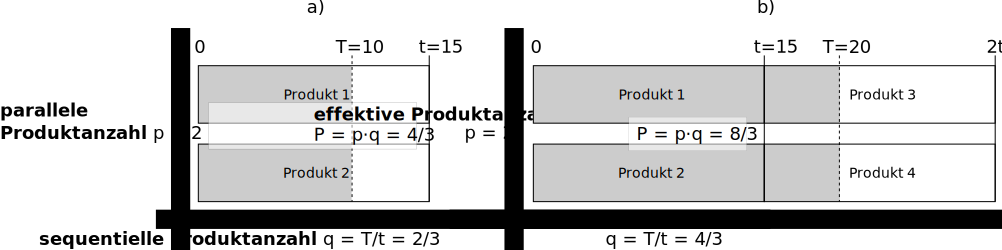
\includegraphics[width=\textwidth]{Produktanzahlen}
			\caption{Veranschaulichung des Zusammenhangs zwischen paralleler, sequentieller und effektiver Produktanzahl. In Fall a) ist der Betrachtungszeitraum $T$ kürzer als die Nutzungsdauer $t$, sodass die zwei parallel eingesetzten Produkte nur anteilig auf das Nutzungssystem angerechnet werden. In Fall b) ist der Betrachtungszeitraum länger als die Nutzungsdauer, sodass zwei Produkte voll und zwei weitere anteilig angerechnet werden.}
			\label{fig:Produktanzahlen}
		\end{figure}
		
		Die oben eingeführte Produktnutzungsdauer $t$ ist eine entscheidende Größe für den Umweltverbrauch eines Produktnutzungssystems: Je länger ein Produkt in der Nutzung ist, desto mehr Service kann es unter sonst gleichen Umständen generieren, sodass sich die produktbezogenen Inputs gemäß der MIPS-Gleichung (\ref{eq:MIPS}) auf eine größere Servicemenge verteilen. 
		
		Die Nutzungsdauer eines Produkts wird durch den Zeitpunkt seiner Entsorgung bestimmt. Es kann zahlreiche Gründe geben, weshalb ein Produkt entsorgt wird. Wir unterscheiden im Modell zwei charakteristische Fälle: eine zeitlich bedingte Entsorgung und eine nutzungsbedingte Entsorgung.
		
		Eine zeitlich bedingte Entsorgung tritt auf, wenn ein Produkt nach einer gewissen Zeitdauer trotz eventuell gegebener Funktionstüchtigkeit den aktuellen technischen, ästhetischen oder sonstigen Anforderungen nicht mehr genügt. Diese Zeitdauer bezeichnen wir als Maximalnutzungsdauer $t_\text{max}$, die unabhängig davon ist, ob und wie intensiv ein Produkt genutzt wird. Sie hängt neben äußeren Rahmenbedingungen, wie dem technischen Fortschritt oder Modezyklen, in hohem Maße vom Verhalten der Nutzer\_innen ab und kann daher zu einem gewissen Grad bewusst beeinflusst werden (vgl. Kapitel \ref{sec:Reparatur}).
		
		Zu einer nutzungsbedingten Entsorgung hingegen kommt es, wenn das Produkt aufgrund von Abnutzung und damit einhergehenden Defekten nicht mehr funktionstüchtig ist. Dies bilden wir im Modell durch eine gewisse Maximalanzahl an Nutzungen ab, die ein Produkt insgesamt zur Verfügung stellt -- den Nutzungsvorrat $n_\text{max}$. Bei einer gegebenen Nutzungshäufigkeit $h$, die angibt wie oft ein Produkt pro Zeit genutzt wird, lässt sich der Nutzungsvorrat in die technische Lebensdauer $t_\text{tech}$ übersetzen:
		%
		\begin{equation}
			\label{eq:t_tech}
			t_\text{tech} = \frac{n_\text{max}}{h}
		\end{equation}
		%
		So würde beispielsweise eine Waschmaschine, die $n_\text{max} = 1.560 \text{ Waschgänge}$ zur Verfügung stellt und mit der Nutzungshäufigkeit $h = 2 \textfrac{Waschgänge}{Woche}$ zum Einsatz kommt, eine technische Lebensdauer von $t_\text{tech} = \frac{1.560}{2} \text{ Wochen} = 15 \text{ Jahre}$ erreichen.
		
		Ausschlaggebend für die Produktnutzungsdauer ist, welcher der beiden genannten Gründe für eine Entsorgung zuerst eintritt. Mit anderen Worten: Ein Produkt verbleibt genau so lange in der Nutzungsphase, bis es entweder nicht mehr benötigt wird oder nicht mehr funktionstüchtig ist. Als Gleichung formulieren wir:
		\begin{equation}
			t = \text{min} \{t_\text{max}, t_\text{tech}\}
		\end{equation}
		%
		%Dies lässt sich mit Gleichung \ref{eq:t_tech} auch schreiben als:
		%\begin{equation}
		%	\label{eq:t_Fallunterscheidung}
		%	t =\left\{\begin{array}{ll}  t_{\text{max}} & \mbox{falls } t_{\text{max}} < \frac{n_{\text{max}}}{h} \\ \frac{n_{\text{max}}}{h} & \mbox{sonst} \end{array}\right.
		%\end{equation} \noteJ{Gleichung \ref{eq:t_Fallunterscheidung} evt. weglassen}
		
		Nachdem nun die Produktanzahl $P$ und damit zusammenhängend die Produktnutzungsdauer $t$ hinreichend spezifiziert worden sind, kommen wir zur Nutzungsmenge $N$.
		
		Die Nutzungsmenge $N$ gibt an, wie viele Nutzungseinheiten innerhalb des Betrachtungszeitraums von allen Produkten des Nutzungssystems insgesamt abgerufen werden. Sie hängt unmittelbar mit der Service-Menge $S$ zusammen, da jede Produktnutzung einen gewissen Service bereitstellt. Die Service-Menge, die mit einer Nutzungseinheit einhergeht, bezeichnen wir als absolute Produktauslastung $A$. Somit gilt:
		\begin{equation}
			\label{eq:S(N,A)}
			S = N \cdot A
		\end{equation}
		
		Es gibt Produkte, die eine variable Service-Menge je Nutzungseinheit bereitstellen können, je nachdem wie stark sie bei der Nutzung ausgelastet sind. Die absolute Produktauslastung kann hier beispielsweise durch den Beladungsgrad einer Maschine gegeben sein. Gibt es eine maximale Produktauslastung, die wir als Kapazität $K$ bezeichnen, kann zu einer Betrachtung der relativen Produktauslastung $a$ übergegangen werden:
		\begin{equation}
		\label{eq:a(A,K)}
		a = \frac{A}{K}
		\end{equation}
		%
		So ist beispielsweise eine Waschmaschine, die über eine Kapazität von $K = 7 ~ \frac{\text{kg}}{\text{Waschgang}}$ verfügt und mit $A = 3.5 ~ \frac{\text{kg}}{\text{Waschgang}}$ Wäsche beladen ist, genau zur Hälfte ausgelastet, das heißt $a = 0.5$. Wir fassen die Gleichungen \ref{eq:S(N,A)} und \ref{eq:a(A,K)} zusammen, und stellen nach $N$ um:
		\begin{equation}
			N = \frac{S}{a \cdot K}
		\end{equation}
		
		Andere Produkte stellen stets die gleiche Service-Menge je Nutzungseinheit bereit. Hier kann die absolute Produktauslastung als konstant angesehen werden, wobei der Begriff \enquote{Auslastung} in diesem Fall ein wenig irreführend ist und stattdessen besser von Nutzungs-Leistung die Rede sein sollte. Beispielsweise kann mit einer Bohrmaschine immer nur ein Loch zur gleichen Zeit gebohrt werden. Wird etwa als Nutzungseinheit \enquote{eine Minute bohren} angesetzt, und können in einer Minute durchschnittlich 2 Löcher gebohrt werden, ergibt sich eine konstante \enquote{Auslastung} bzw. Nutzungs-Leistung von $A = 2 ~ \frac{\text{Löcher}}{\text{Minute bohren}}$.
		
		Eine alternative Bestimmung der Nutzungsmenge $N$ eines Nutzungssystems ergibt sich aus der Produktnutzungsmenge $n$ eines einzelnen Produkts. Diese bezieht sich auf den gesamten Lebenszyklus eines Produkts und wird durch die Nutzungsdauer $t$ und die Nutzungshäufigkeit $h$ bestimmt:
		\begin{equation}
			n = h \cdot t
		\end{equation}
		%
		Durch Multiplikation mit der oben eingeführten effektiven Produktanzahl $P$ ergibt sich die Nutzungsmenge $N$ des Nutzungssystems:
		\begin{equation}
			N = h \cdot t \cdot P
		\end{equation}

		\subsection{Effektive Größen, Mittelwerte}
		\noteS{nur ein ganz fixer erster Entwurf}Für die Berechnung des MIPS müssen die innerhalb der Systemgrenzen (die u.a.
		durch eine Zeit $T$ charakterisiert sind) anfallenden
		Material-Inputs durch die abgerufene Servicemenge geteilt werden:
		\begin{equation}
		  \MIPS = \frac{I}{S}
		\end{equation}
		Die Effekte kollektiver Nutzung lassen sich in Mengeneffekte und
		Nachfrageeffekte einteilen. Um die beiden Effekte mathematisch sauber
		voneinander abzugrenzen, führen wir einen konstanten Betrachtungszeitraum
		$\T{eff}$
		ein, innerhalb dessen eine bestimmte Servicemenge $S_D$ nachgefragt wird.
		Mengeneffekte sind nun gerade dadurch charakterisiert, dass $S_D =
		\text{konst}$ gilt. Beim Übergang zu $\T{eff}$ müssen wir berücksichtigen, dass
		wir
		nur einen bestimmten Anteil der innerhalb der Systemgrenzen anfallenden
		Material-Inputs anrechnen müssen. Wir nennen diesen Anteil die effektiven
		Material-Inputs $\I{eff}$. Es ergibt sich also:
		\begin{equation}
		  \MIPS = \frac{I}{S} = \frac{\I{eff}}{S_D}
		\end{equation}
		Wir betrachten nun die effektiven Material-Inputs, die sich durch Mengeneffekte
		ändern können. Deren Anteil an den gesamten Material-Inputs entspricht dem
		Verhältnis Betrachtungszeitraum zum gesamt Zeitraum des Nutzungssystems
		$\frac{\T{eff}}{T}$, sie können also folgendermaßen berechnet werden:
		\begin{equation}
		  \I{eff} = I \cdot \frac{\T{eff}}{T}
		\end{equation}
		Die Material-Inputs können wir in nutzungsbedingte Inputs $I_N$, produktbezogene
		Inputs $I_P$ und von den Anzahl der Nutzungen und Produkte innerhalb des Systems
		unabhängige Inputs $\I{fix}$ einteilen.
		Die ersten beiden Inputs berechnen sich als Summe über die Inputs bei jeder
		Nutzung $i_N^k$ bzw. die Inputs für jedes Produkt $i_P^k$:
		\begin{align}
		  I_P &= \sum_k^P i_P^k = P \cdot \overline{i_P}\\
		  I_N &= \sum_k^N i_N^k = N \cdot \overline{i_N}
		\end{align}
		Hierbei bezeichnet $P$ die Produktanzahl im System und $N$ die Anzahl der
		Nutzungen. Die Summen wurden in die alternative Schreibweise mit 
		Durchschnittswerten umgeformt. Die effektiven Inputs lassen sich nun
		folgendermaßen berechnen:
		\begin{equation}
		  \I{eff} = \frac{\T{eff}}{T} \cdot I 
		          = \frac{\T{eff}}{T} \cdot (N \cdot \overline{i_N} + P \cdot
		          \overline{i_P} + \I{fix})
		\end{equation}
		Wir können in einem letzten Schritt zur effektiven Nutzungsmenge, effektiven
		Produktmenge und effektiven fixen Inputs übergehen, indem wir definieren:
		\begin{align}
		  \N{eff} &\defeq N \cdot \frac{\T{eff}}{T} \\
		  \P{eff} &\defeq P \cdot \frac{\T{eff}}{T} \\
		  \I{fix, eff} &\defeq \I{fix} \cdot \frac{\T{eff}}{T} 
		\end{align}
		Natürlich stellt sich die Frage, wie diese effektiven Größen bestimmt werden
		können. Für den Fall der Nutzungsmenge ist dies einfach: die effektive
		Nutzungsmenge ist einfach die Nutzungsmenge, die im Betrachtungszeitraum
		$\T{eff}$ anfällt und ergibt sich damit direkt aus der Servicemenge $S_D$. Die
		effektive Produktmenge kann unter der Annahme identischer Nutzungsdauern $t$ und
		der Kenntnis der parallel genutzten Produkte $p$ wie folgt bestimmt werden:
		\begin{equation}
		  \P{eff} = \frac{\T{eff}}{t} \cdot p = \frac{\N{eff}}{h \cdot t}
		\end{equation}
		Letztlich können die effektiven fixen Inputs unter der Annahme, dass dafür pro
		Zeiteinheit $\itext{fix} = \frac{\I{fix}}{T}$ viele Inputs anfallen, so bestimmt
		werden:
		\begin{equation}
		  \I{fix, eff} = T \cdot \itext{fix} = \text{konst}
		\end{equation}
		
		Insgesamt lässt sich also schreiben: 
		\begin{equation}
		  \I{eff} = \N{eff} \cdot \overline{i_N} + \P{eff} \cdot
		          \overline{i_P} + \I{fix, eff}
		          = \frac{S_D}{A} \cdot \overline{i_N} + \frac{\N{eff}}{h \cdot t} \cdot
		          \overline{i_P} + \T{eff} \cdot \itext{fix}
		          \label{eq:Grundmodell}
		\end{equation}
		
		Wir haben also eine Gleichung erhalten, die nur noch effektive und
		durchschnittliche Werte beinhalten. Diese Gleichung verwenden wir im folgenden
		bei der Modellierung der Teileffekte, und lassen dabei den Index "`eff"' sowie
		den Durchschnitts-Querstrich weg, da wir diese nicht mehr von den realen Größen
		unterscheiden müssen. 
		\section{Einzeleffekte}
		\label{sec:Einzeleffekte}
			\subsection{Nutzungsintensivierung} % Ursprünglich: "Nutzungsdauerverlängerung"
			\label{sec:Nutzungsintensivierung}
				\paragraph{Modellbeschreibung}
				Unter \enquote{Nutzungsintensivierung} verstehen wir eine Erhöhung der Häufigkeit, mit der ein bestimmtes Produkt genutzt wird. Diese bezeichnen wir als Nutzungshäufigkeit $h$ und definieren sie als die Produktnutzungsmenge pro Zeit. Für eine Waschmaschine wäre dies etwa die Anzahl an Waschgängen pro Woche.
				
				Ein Produkt wird während seines Lebenszyklus eine bestimmte Zeitperiode lang genutzt. Diese Zeitspanne zwischen Anschaffung bis Entsorgung wird als Nutzungsdauer $t$ bezeichnet. Aus der Nutzungshäufigkeit $h$ und der Nutzungsdauer $t$ ergibt sich die Nutzungsmenge $n$ eines einzelnen Produkts:
	%
				\begin{equation}
					\label{eq:n(h)}
					n (h) = h \cdot t
				\end{equation}
	%
				So stellt beispielsweise eine Waschmaschine, die zwei mal pro Woche genutzt wird, in einer Nutzungsdauer von 15 Jahren $n = 2 \textfrac{Waschgänge}{Woche} \cdot 52 \textfrac{Wochen}{Jahr} \cdot 15 \text{ Jahre} = 1560$ Waschgänge zur Verfügung.
	
				Werden $P$ Produkte in einem Produktnutzungssystem eingesetzt, ergibt sich die Gesamtnutzungsmenge
	%
				\begin{equation}
					\label{eq:N(h)}
					N = n \cdot P = h \cdot t \cdot P
				\end{equation}
	%
				Hierbei ist zu beachten, dass die effektive Produktanzahl $P$ sowohl gleichzeitig, als auch nacheinander eingesetzte Produkte berücksichtigt. Die Anzahl der gleichzeitig eingesetzten Produkte bezeichnen wir als parallele Produktanzahl $p$, was stets eine natürliche Zahl ist. Demgegenüber verstehen wird unter der sequentiellen Produktanzahl $q$ die Anzahl der Produkte, die innerhalb des Betrachtungszeitraums nacheinander eingesetzt werden. Diese Größe muss nicht ganzzahlig sein, da ein Produkt auch anteilig dem betrachteten Nutzungssystem angerechnet werden kann, wenn es innerhalb des Betrachtungszeitraums nur einen Teil seines Nutzungsvorrats zur Verfügung stellt und der Rest auf eine vorausgegangene oder nachfolgende Nutzung entfällt. Diese Eigenschaft überträgt sich auf die effektive Produktanzahl $P$, wie das folgende Beispiel illustriert: Werden in einem Gemeinschaftswaschkeller im Betrachtungszeitraum $T  = 10 \text{ Jahren}$ parallel $p = 2$ Maschinen betrieben, die jeweils über eine Nutzungsdauer von $t = 15 \text{ Jahren}$ verfügen, so sind sie jeweils nur zu $q = \nicefrac{10}{15}$ dem betrachteten Nutzungssystem anzurechnen, sodass sich eine Produktanzahl von $P = 2 \cdot \nicefrac{10}{15} \approx 1.33$ ergibt. Für den Fall, dass der Betrachtungszeitraum $T$ hingegen länger ist als die Nutzungsdauer $t$, muss jedes parallel eingesetzte Produkt mehr als einmal angerechnet werden, da es innerhalb des Betrachtungszeitraums ersetzt werden muss: So würden im obigen Beispiel in einem Zeitraum von $T  = 20 \text{ Jahren}$ eine Anzahl von $P = 2 \cdot \nicefrac{20}{15} \approx 2.67$ Maschinen eingesetzt werden. Abbildung \ref{fig:Produktanzahlen} stellt die beiden Zahlenbeispiele grafisch dar.
				
				Allgemein gilt:
	%
				\begin{equation}
					\label{eq:P(p)}
					P = p \cdot q = p \cdot \frac{T}{t}
				\end{equation}
	%
				 \begin{figure}[ht]
				 	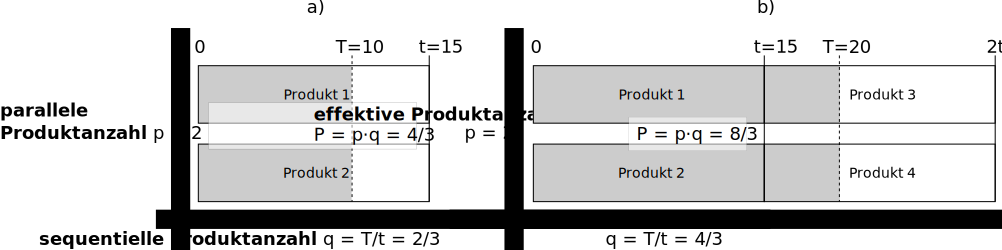
\includegraphics[width=\textwidth]{Produktanzahlen}
				 	\caption{Veranschaulichung des Zusammenhangs zwischen paralleler, sequentieller und effektiver Produktanzahl. In Fall a) ist der Betrachtungszeitraum $T$ kürzer als die Nutzungsdauer $t$, sodass die zwei parallel eingesetzten Produkte nur anteilig auf das Nutzungssystem angerechnet werden. In Fall b) ist der Betrachtungszeitraum länger als die Nutzungsdauer, sodass zwei Produkte voll und zwei weitere anteilig angerechnet werden.}
					\label{fig:Produktanzahlen}
				 \end{figure}
				 \noteJ{Abbildung schön machen: Text in LaTeX}
	
				Dabei ist zu beachten, dass die parallele Produktanzahl $p$ eine Nutzungssystem-spezifische Mindestproduktanzahl $p_\text{min}$ nicht unterschreitet. Die Mindestproduktanzahl kann beispielsweise dadurch erforderlich sein, dass aus praktisch-organisatorischen Gründen zu Stoßzeiten eine gewisse Anzahl an Produkten gleichzeitig im Einsatz ist. Als Formel:
	%
				\begin{equation}
					\label{eq:p_min}
					p \geq p_{\text{min}} \qquad  p, p_{\text{min}} \in \mathbb{N}
				\end{equation}			
				
				Bei einer gegebenen absoluten Produktauslastung $A$, deren Einfluss im Teilmodell \enquote{\nameref{sec:Produktauslastung}} (Kapitel \ref{sec:Produktauslastung}) ausführlich untersucht wird, bestimmt sich die Service-Menge $S$ durch
	%
				\begin{equation}
				\label{eq:S(A)}
					S = N \cdot A
				\end{equation}
	%			
				Die Service-Menge lässt sich jedoch auch von der Nachfrageseite her betrachten: In einem konkreten Nutzungssystem besteht eine bestimmte Nachfrage nach Service. Diese wird von der Anzahl der Personen, dem individuellen Servicebedarf und dem Betrachtungszeitraum abhängen, was in diesem Teil-Modell jedoch nicht weiter von Belang ist, da diese Größen in Bezug auf die Nutzungshäufigkeit als konstant angenommen werden können. Insofern stellt die Service-Nachfrage $S_D$ hier eine Konstante dar und es ergibt sich eine zweite Bestimmungsgleichung:
				%
				\begin{equation}
				\label{eq:S_D}
				S = S_D
				\end{equation}
				%
				Somit ist die Gesamtnutzungsmenge $N$ durch den hier als konstant betrachteten Ausdruck
	%
				\begin{equation}
					\label{eq:N(S_D)}
					N = \frac{S_D}{A}
				\end{equation}
	%						
				gegeben. Betrachtet man Gleichung \ref{eq:N(h)} ($N (h) = h \cdot t \cdot P$) unter diesem Gesichtspunkt, so wird deutlich, dass eine Erhöhung der Nutzungshäufigkeit $h$ bei gleichbleibender Produktnutzungsdauer $t$ zu einer geringeren effektiven Produktanzahl $P$ führt. Hierin besteht der positive Umwelteffekt der Nutzungsintensivierung, da weniger Produkte für die gleiche Servicemenge hergestellt und entsorgt werden müssen.
				
				Umgekehrt wird eine Erhöhung der Nutzungshäufigkeit bei kollektiver Nutzung gerade durch eine Reduktion der Produktanzahl erreicht: Teilen sich beispielsweise mehrere Personen eine Waschmaschine, anstatt jeweils eine eigene zu besitzen, erhöht sich die Häufigkeit, mit der die Maschine betrieben wird. Genauer gesagt ist die Nutzungshäufigkeit $h$ für ein Nutzungssystem mit gegebener Service-Nachfrage $S_D$, gegebener Produktauslastung $A$ und einem festen Betrachtungszeitraum $T$ von der parallelen Produktanzahl $p$ abhängig: Je weniger Produkte parallel im Einsatz sind, desto häufiger müssen diese genutzt werden um die Nachfrage zu bedienen. Dieser Zusammenhang lässt sich formal folgendermaßen nachvollziehen:
	%
				\begin{equation*}
					h \eqnref{eq:N(h)} \frac{N}{t \cdot P} \eqnref{eq:P(p)} \frac{N}{t \cdot p \cdot \frac{T}{t}}
					= \frac{N}{p \cdot T} \eqnref{eq:N(S_D)} \frac{S_D}{A \cdot p \cdot T} \qquad p \in \mathbb{N}
				\end{equation*}
	%
				Die Nutzungshäufigkeit ist also reziprok proportional zur parallelen Produktanzahl $p$. Da es sich bei $p$ um eine natürliche Zahl handelt, kann in dem betrachteten Szenario auch die Nutzungshäufigkeit $h$ nur diskrete Werte annehmen. Durch die Beschränkung von $p$ durch $p_\text{min}$ gemäß Gleichung \ref{eq:p_min} ergibt sich zudem eine Maximalnutzungshäufigkeit $h_\text{max}$:
	%
				\begin{equation*}
					h = \frac{S_D}{A \cdot p \cdot T} \leq \frac{S_D}{A \cdot p_\text{min} \cdot T} =: h_\text{max}
				\end{equation*}
				
				Nach diesen einschränkenden Bemerkungen zur Nutzungshäufigkeit wenden wir uns nun wieder der effektiven Produktanzahl $P$ zu. Weiter oben wurde bereits der Einfluss der Nutzungshäufigkeit $h$ auf die Produktanzahl $P$ bei gleichbleibender Produktnutzungsdauer $t$ untersucht. Letztere ist allerdings nicht in jedem Fall gegeben, wie im Folgenden gezeigt wird.
				
				Die Nutzungsdauer $t$ eines Produkts wird durch die folgenden zwei Zusammenhänge bestimmt: Einerseits stellt das Produkt Verschleiß"=bedingt nur eine bestimmte Produktnutzungsmenge -- den Einzelnutzungsvorrat \noteJ{Bezeichnung Einzelnutzungsvorrat unschön} $n_{\text{max}}$ -- zur Verfügung und wird nach dessen Aufbrauchen entsorgt. Andererseits kann das Produkt auch bei voller Funktionsfähigkeit nach einer gewissen Zeit aus dem Verkehr gezogen werden, wenn es etwa aktuellen technischen oder modischen Standards nicht mehr genügt. Diese Zeit ist von der Nutzung unabhängig und wird hier als Maximalnutzungsdauer $t_{\text{max}}$ bezeichnet. Formal lassen sich diese Zusammenhänge als zwei Bedingungen formulieren:
	%
				\begin{equation*}
					n \leq n_{\text{max}}
				\end{equation*}
	%			
				\begin{equation*}	
					t \leq t_{\text{max}}
				\end{equation*}	
	%
				Die erste Bedingung impliziert unter Berücksichtigung von Gleichung \ref{eq:n(h)}:
				\begin{equation*}	
					t = \frac{n}{h} \leq \frac{n_{\text{max}}}{h} =: t_\text{tech}(h)
				\end{equation*}
	%
				Dabei bezeichnet $t_\text{tech}(h$) die von der Nutzungshäufigkeit abhängige technische Lebensdauer. Es ist davon auszugehen, dass ein Produkt so lange genutzt wird, bis entweder die technische Lebensdauer, oder die Maximalnutzungsdauer erreicht wird. Damit lässt sich die Nutzungsdauer folgendermaßen bestimmen:
	%			
				\begin{equation*}	
					t (h) = \min \left\{ t_{\text{max}}, t_\text{tech}(h) \right\}
				\end{equation*}	
	%			
				Dies ist gleichbedeutend zu:
	%			
				\begin{equation*}	
					t (h) =\left\{\begin{array}{ll}  t_{\text{max}} & \mbox{falls } h <  \frac{n_{\text{max}}}{t_{\text{max}}} =: h^* \\ \frac{n_{\text{max}}}{h} & \mbox{sonst} \end{array}\right.
				\end{equation*}	
	%
				Solange also die Nutzungshäufigkeit zu gering ist um den Nutzungsvorrat innerhalb der Maximalnutzungsdauer aufzubrauchen ($h < h*$), ist die Nutzungsdauer durch die Maximalnutzungsdauer $t_{\text{max}}$ gegeben. Bei einer höheren Nutzungshäufigkeit ist hingegen die technische Lebensdauer $\frac{n_{\text{max}}}{h}$ ausschlaggebend, die mit zunehmender Nutzungshäufigkeit antiproportional abnimmt, da der Nutzungsvorrat schneller aufgebraucht wird.
				
				Für die Nutzungsmenge $n$ eines Produkts ergibt sich hieraus mit Gleichung \ref{eq:n(h)}:
	%			
				\begin{equation}
					\label{eq:n(h)_cases}
					n (h) = h \cdot t(h) = \left\{\begin{array}{ll}  h \cdot t_{\text{max}} & \mbox{falls } h < h^* \\ n_{\text{max}} & \mbox{sonst} \end{array}\right.
				\end{equation}	
	%			
				Hier verhält es sich also umgekehrt als bei der Nutzungsdauer: Solange der Nutzungsvorrat innerhalb der Maximalnutzungsdauer aufgrund einer geringen Nutzungshäufigkeit nicht aufgebraucht wird ($h < h^*$), ist die Nutzungsmenge proportional von der Nutzungshäufigkeit abhängig, weil das Produkt in derselben Zeit häufiger genutzt wird: $n (h) = h \cdot t_{\text{max}}$. Bei einer höheren Nutzungshäufigkeit bleibt die Nutzungsmenge hingegen konstant auf dem Niveau des Nutzungsvorrats $n_{\text{max}}$, weil das Produkt nicht darüber hinaus genutzt werden kann.
				
				Mit Gleichung \ref{eq:N(h)} ($N = n \cdot P$) lässt sich schließlich die effektive Produktanzahl $P(h)$ bestimmen:
	%			
				\begin{equation}
				\label{eq:P(h)}	
					P (h) = \frac{N}{n(h)} = \left\{\begin{array}{ll}  \frac{N}{h \cdot t_{\text{max}}} & \mbox{falls } h < h^* \\[5pt] \frac{N}{n_{\text{max}}} & \mbox{sonst} \end{array}\right.
				\end{equation}	
				
				Wiederum ist der Punkt, an dem die Nutzungshäufigkeit gerade so groß ist, dass der Nutzungsvorrat innerhalb der Maximalnutzungsdauer aufgebraucht wird ($h = h*$), entscheidend: Bei geringerer Nutzungshäufigkeit ist die benötigte Produktanzahl antiproportional zur Nutzungshäufigkeit, bei höherer Nutzungshäufigkeit ist sie hingegen konstant. Dies folgt direkt aus den eben gemachten Beobachtungen zur Nutzungsmenge n(h)und hat zur Folge, dass eine Nutzungsintensivierung nur solange einen positiven Umwelteffekt aufweist, bis der Nutzungsvorrat voll ausgeschöpft wird, was noch im Detail gezeigt werden wird.
				
				Abbildung \ref{fig:t(h)_n(h)_P(h)} stellt die Abhängigkeiten der Nutzungsdauer $t$, der Nutzungsmenge $n$ und der Produktanzahl $P$ von der Nutzungshäufigkeit $h$ dar.
				
				\begin{figure}[ht]
					\centering
					% Created by tikzDevice version 0.8.1 on 2015-08-28 10:31:17
% !TEX encoding = UTF-8 Unicode
\begin{tikzpicture}[x=1pt,y=1pt]
\definecolor{fillColor}{RGB}{255,255,255}
\path[use as bounding box,fill=fillColor,fill opacity=0.00] (0,0) rectangle (433.62,180.67);
\begin{scope}
\path[clip] ( 32.47, 48.31) rectangle (127.91,129.19);
\definecolor{drawColor}{RGB}{190,190,190}

\path[draw=drawColor,line width= 0.4pt,line join=round,line cap=round] (124.37, 76.27) --
	(120.55, 77.40) --
	(117.04, 78.53) --
	(113.82, 79.66) --
	(110.84, 80.79) --
	(108.08, 81.92) --
	(105.51, 83.05) --
	(103.12, 84.17) --
	(100.90, 85.30) --
	( 98.81, 86.43) --
	( 96.85, 87.56) --
	( 95.02, 88.69) --
	( 93.29, 89.82) --
	( 91.66, 90.95) --
	( 90.11, 92.08) --
	( 88.66, 93.21) --
	( 87.27, 94.34) --
	( 85.96, 95.46) --
	( 84.72, 96.59) --
	( 83.53, 97.72) --
	( 82.40, 98.85) --
	( 81.33, 99.98) --
	( 80.30,101.11) --
	( 79.32,102.24) --
	( 78.38,103.37) --
	( 77.48,104.50) --
	( 76.62,105.63) --
	( 75.79,106.76) --
	( 75.00,107.88) --
	( 74.23,109.01) --
	( 73.50,110.14) --
	( 72.80,111.27) --
	( 72.12,112.40) --
	( 71.46,113.53) --
	( 70.83,114.66) --
	( 70.22,115.79) --
	( 69.63,116.92) --
	( 69.06,118.05) --
	( 68.51,119.17) --
	( 67.98,120.30) --
	( 67.46,121.43) --
	( 66.97,122.56) --
	( 66.48,123.69) --
	( 66.02,124.82) --
	( 65.56,125.95) --
	( 65.12,126.20) --
	( 64.69,126.20) --
	( 64.28,126.20) --
	( 63.88,126.20) --
	( 63.48,126.20) --
	( 63.10,126.20) --
	( 62.73,126.20) --
	( 62.37,126.20) --
	( 62.02,126.20) --
	( 61.68,126.20) --
	( 61.35,126.20) --
	( 61.02,126.20) --
	( 60.70,126.20) --
	( 60.40,126.20) --
	( 60.10,126.20) --
	( 59.80,126.20) --
	( 59.52,126.20) --
	( 59.24,126.20) --
	( 58.96,126.20) --
	( 58.70,126.20) --
	( 58.44,126.20) --
	( 58.18,126.20) --
	( 57.93,126.20) --
	( 57.69,126.20) --
	( 57.45,126.20) --
	( 57.22,126.20) --
	( 56.99,126.20) --
	( 56.77,126.20) --
	( 56.55,126.20) --
	( 56.34,126.20) --
	( 56.13,126.20) --
	( 55.92,126.20) --
	( 55.72,126.20) --
	( 55.52,126.20) --
	( 55.33,126.20) --
	( 55.14,126.20) --
	( 54.96,126.20) --
	( 54.77,126.20) --
	( 54.60,126.20) --
	( 54.42,126.20) --
	( 54.25,126.20) --
	( 54.08,126.20) --
	( 53.91,126.20) --
	( 53.75,126.20) --
	( 53.59,126.20) --
	( 53.43,126.20) --
	( 53.28,126.20) --
	( 53.13,126.20) --
	( 52.98,126.20) --
	( 52.83,126.20) --
	( 52.69,126.20) --
	( 52.55,126.20) --
	( 52.41,126.20) --
	( 52.27,126.20) --
	( 52.14,126.20) --
	( 52.01,126.20) --
	( 51.88,126.20) --
	( 51.75,126.20) --
	( 51.62,126.20) --
	( 51.50,126.20) --
	( 51.38,126.20) --
	( 51.26,126.20) --
	( 51.14,126.20) --
	( 51.02,126.20) --
	( 50.91,126.20) --
	( 50.80,126.20) --
	( 50.69,126.20) --
	( 50.58,126.20) --
	( 50.47,126.20) --
	( 50.36,126.20) --
	( 50.26,126.20) --
	( 50.15,126.20) --
	( 50.05,126.20) --
	( 49.95,126.20) --
	( 49.85,126.20) --
	( 49.76,126.20) --
	( 49.66,126.20) --
	( 49.56,126.20) --
	( 49.47,126.20) --
	( 49.38,126.20) --
	( 49.29,126.20) --
	( 49.20,126.20) --
	( 49.11,126.20) --
	( 49.02,126.20) --
	( 48.94,126.20) --
	( 48.85,126.20) --
	( 48.77,126.20) --
	( 48.69,126.20) --
	( 48.60,126.20) --
	( 48.52,126.20) --
	( 48.44,126.20) --
	( 48.36,126.20) --
	( 48.29,126.20) --
	( 48.21,126.20) --
	( 48.13,126.20) --
	( 48.06,126.20) --
	( 47.99,126.20) --
	( 47.91,126.20) --
	( 47.84,126.20) --
	( 47.77,126.20) --
	( 47.70,126.20) --
	( 47.63,126.20) --
	( 47.56,126.20) --
	( 47.49,126.20) --
	( 47.43,126.20) --
	( 47.36,126.20) --
	( 47.29,126.20) --
	( 47.23,126.20) --
	( 47.16,126.20) --
	( 47.10,126.20) --
	( 47.04,126.20) --
	( 46.98,126.20) --
	( 46.92,126.20) --
	( 46.85,126.20) --
	( 46.79,126.20) --
	( 46.74,126.20) --
	( 46.68,126.20) --
	( 46.62,126.20) --
	( 46.56,126.20) --
	( 46.51,126.20) --
	( 46.45,126.20) --
	( 46.39,126.20) --
	( 46.34,126.20) --
	( 46.28,126.20) --
	( 46.23,126.20) --
	( 46.18,126.20) --
	( 46.12,126.20) --
	( 46.07,126.20) --
	( 46.02,126.20) --
	( 45.97,126.20) --
	( 45.92,126.20) --
	( 45.87,126.20) --
	( 45.82,126.20) --
	( 45.77,126.20) --
	( 45.72,126.20) --
	( 45.67,126.20) --
	( 45.63,126.20) --
	( 45.58,126.20) --
	( 45.53,126.20) --
	( 45.49,126.20) --
	( 45.44,126.20) --
	( 45.40,126.20) --
	( 45.35,126.20) --
	( 45.31,126.20) --
	( 45.26,126.20) --
	( 45.22,126.20) --
	( 45.18,126.20) --
	( 45.13,126.20) --
	( 45.09,126.20) --
	( 45.05,126.20) --
	( 45.01,126.20) --
	( 44.96,126.20) --
	( 44.92,126.20) --
	( 44.88,126.20) --
	( 44.84,126.20);
\definecolor{drawColor}{RGB}{0,0,0}
\definecolor{fillColor}{RGB}{255,255,255}

\path[draw=drawColor,line width= 0.4pt,line join=round,line cap=round,fill=fillColor] (123.06, 74.96) rectangle (125.69, 77.59);

\path[draw=drawColor,line width= 0.4pt,line join=round,line cap=round,fill=fillColor] ( 78.87, 99.92) rectangle ( 81.51,102.55);

\path[draw=drawColor,line width= 0.4pt,line join=round,line cap=round,fill=fillColor] ( 64.15,124.88) rectangle ( 66.78,127.52);

\path[draw=drawColor,line width= 0.4pt,line join=round,line cap=round,fill=fillColor] ( 56.78,124.88) rectangle ( 59.41,127.52);

\path[draw=drawColor,line width= 0.4pt,line join=round,line cap=round,fill=fillColor] ( 52.36,124.88) rectangle ( 55.00,127.52);

\path[draw=drawColor,line width= 0.4pt,line join=round,line cap=round,fill=fillColor] ( 49.42,124.88) rectangle ( 52.05,127.52);

\path[draw=drawColor,line width= 0.4pt,line join=round,line cap=round,fill=fillColor] ( 47.31,124.88) rectangle ( 49.95,127.52);

\path[draw=drawColor,line width= 0.4pt,line join=round,line cap=round,fill=fillColor] ( 45.74,124.88) rectangle ( 48.37,127.52);

\path[draw=drawColor,line width= 0.4pt,line join=round,line cap=round,fill=fillColor] ( 44.51,124.88) rectangle ( 47.14,127.52);

\path[draw=drawColor,line width= 0.4pt,line join=round,line cap=round,fill=fillColor] ( 43.53,124.88) rectangle ( 46.16,127.52);
\end{scope}
\begin{scope}
\path[clip] (  0.00,  0.00) rectangle (144.54,180.67);
\definecolor{drawColor}{RGB}{0,0,0}

\node[text=drawColor,anchor=base,inner sep=0pt, outer sep=0pt, scale=  0.66] at ( 80.19, 18.22) {Nutzungsh"aufigkeit $h$ [NE/Jahr]};

\node[text=drawColor,rotate= 90.00,anchor=base,inner sep=0pt, outer sep=0pt, scale=  0.66] at (  7.13, 88.75) {Nutzungsdauer $t$ [Jahre]};
\end{scope}
\begin{scope}
\path[clip] ( 32.47, 48.31) rectangle (127.91,129.19);
\definecolor{drawColor}{RGB}{0,0,0}

\path[draw=drawColor,line width= 0.4pt,dash pattern=on 1pt off 3pt ,line join=round,line cap=round] ( 65.46, 48.31) -- ( 65.46,129.19);
\end{scope}
\begin{scope}
\path[clip] (  0.00,  0.00) rectangle (144.54,180.67);
\definecolor{drawColor}{RGB}{0,0,0}

\node[text=drawColor,anchor=base,inner sep=0pt, outer sep=0pt, scale=  0.79] at ( 80.19,164.83) {\bfseries Nutzungsdauer $t(h)$};
\end{scope}
\begin{scope}
\path[clip] (  0.00,  0.00) rectangle (433.62,180.67);
\definecolor{drawColor}{RGB}{0,0,0}

\path[draw=drawColor,line width= 0.4pt,line join=round,line cap=round] ( 36.01, 48.31) -- (124.37, 48.31);

\path[draw=drawColor,line width= 0.4pt,line join=round,line cap=round] ( 36.01, 48.31) -- ( 36.01, 44.35);

\path[draw=drawColor,line width= 0.4pt,line join=round,line cap=round] ( 65.46, 48.31) -- ( 65.46, 44.35);

\path[draw=drawColor,line width= 0.4pt,line join=round,line cap=round] ( 80.19, 48.31) -- ( 80.19, 44.35);

\path[draw=drawColor,line width= 0.4pt,line join=round,line cap=round] (124.37, 48.31) -- (124.37, 44.35);

\node[text=drawColor,anchor=base,inner sep=0pt, outer sep=0pt, scale=  0.66] at ( 36.01, 34.06) {0};

\node[text=drawColor,anchor=base,inner sep=0pt, outer sep=0pt, scale=  0.66] at ( 65.46, 34.06) {$h^*$};

\node[text=drawColor,anchor=base,inner sep=0pt, outer sep=0pt, scale=  0.66] at ( 80.19, 34.06) {500};

\node[text=drawColor,anchor=base,inner sep=0pt, outer sep=0pt, scale=  0.66] at (124.37, 34.06) {1000};

\path[draw=drawColor,line width= 0.4pt,line join=round,line cap=round] ( 32.47, 51.31) -- ( 32.47,126.20);

\path[draw=drawColor,line width= 0.4pt,line join=round,line cap=round] ( 32.47, 51.31) -- ( 28.51, 51.31);

\path[draw=drawColor,line width= 0.4pt,line join=round,line cap=round] ( 32.47, 76.27) -- ( 28.51, 76.27);

\path[draw=drawColor,line width= 0.4pt,line join=round,line cap=round] ( 32.47,101.24) -- ( 28.51,101.24);

\path[draw=drawColor,line width= 0.4pt,line join=round,line cap=round] ( 32.47,126.20) -- ( 28.51,126.20);

\node[text=drawColor,rotate= 90.00,anchor=base,inner sep=0pt, outer sep=0pt, scale=  0.66] at ( 22.97, 51.31) {0};

\node[text=drawColor,rotate= 90.00,anchor=base,inner sep=0pt, outer sep=0pt, scale=  0.66] at ( 22.97, 76.27) {5};

\node[text=drawColor,rotate= 90.00,anchor=base,inner sep=0pt, outer sep=0pt, scale=  0.66] at ( 22.97,101.24) {10};

\node[text=drawColor,rotate= 90.00,anchor=base,inner sep=0pt, outer sep=0pt, scale=  0.66] at ( 22.97,126.20) {15};

\path[draw=drawColor,line width= 0.4pt,line join=round,line cap=round] ( 44.84,129.19) -- (124.37,129.19);

\path[draw=drawColor,line width= 0.4pt,line join=round,line cap=round] ( 44.84,129.19) -- ( 44.84,133.15);

\path[draw=drawColor,line width= 0.4pt,line join=round,line cap=round] ( 45.83,129.19) -- ( 45.83,133.15);

\path[draw=drawColor,line width= 0.4pt,line join=round,line cap=round] ( 47.05,129.19) -- ( 47.05,133.15);

\path[draw=drawColor,line width= 0.4pt,line join=round,line cap=round] ( 48.63,129.19) -- ( 48.63,133.15);

\path[draw=drawColor,line width= 0.4pt,line join=round,line cap=round] ( 50.73,129.19) -- ( 50.73,133.15);

\path[draw=drawColor,line width= 0.4pt,line join=round,line cap=round] ( 53.68,129.19) -- ( 53.68,133.15);

\path[draw=drawColor,line width= 0.4pt,line join=round,line cap=round] ( 58.10,129.19) -- ( 58.10,133.15);

\path[draw=drawColor,line width= 0.4pt,line join=round,line cap=round] ( 65.46,129.19) -- ( 65.46,133.15);

\path[draw=drawColor,line width= 0.4pt,line join=round,line cap=round] ( 80.19,129.19) -- ( 80.19,133.15);

\path[draw=drawColor,line width= 0.4pt,line join=round,line cap=round] (124.37,129.19) -- (124.37,133.15);

\node[text=drawColor,anchor=base,inner sep=0pt, outer sep=0pt, scale=  0.66] at ( 44.84,138.70) {10};

\node[text=drawColor,anchor=base,inner sep=0pt, outer sep=0pt, scale=  0.66] at ( 58.10,138.70) {4};

\node[text=drawColor,anchor=base,inner sep=0pt, outer sep=0pt, scale=  0.66] at ( 80.19,138.70) {2};

\node[text=drawColor,anchor=base,inner sep=0pt, outer sep=0pt, scale=  0.66] at (124.37,138.70) {1};

\path[draw=drawColor,line width= 0.4pt,line join=round,line cap=round] ( 32.47, 48.31) --
	(127.91, 48.31) --
	(127.91,129.19) --
	( 32.47,129.19) --
	( 32.47, 48.31);

\node[text=drawColor,anchor=base,inner sep=0pt, outer sep=0pt, scale=  0.66] at ( 80.19,150.58) {parallele Produktanzahl $p$};

\node[text=drawColor,anchor=base,inner sep=0pt, outer sep=0pt, scale=  1.00] at ( 80.19,  2.38) {(a)};
\end{scope}
\begin{scope}
\path[clip] (177.01, 48.31) rectangle (272.45,129.19);
\definecolor{drawColor}{RGB}{190,190,190}

\path[draw=drawColor,line width= 0.4pt,line join=round,line cap=round] (268.91,126.20) --
	(265.09,126.20) --
	(261.58,126.20) --
	(258.36,126.20) --
	(255.38,126.20) --
	(252.62,126.20) --
	(250.05,126.20) --
	(247.66,126.20) --
	(245.44,126.20) --
	(243.35,126.20) --
	(241.39,126.20) --
	(239.56,126.20) --
	(237.83,126.20) --
	(236.20,126.20) --
	(234.65,126.20) --
	(233.20,126.20) --
	(231.81,126.20) --
	(230.50,126.20) --
	(229.26,126.20) --
	(228.07,126.20) --
	(226.94,126.20) --
	(225.87,126.20) --
	(224.84,126.20) --
	(223.86,126.20) --
	(222.92,126.20) --
	(222.02,126.20) --
	(221.16,126.20) --
	(220.33,126.20) --
	(219.54,126.20) --
	(218.77,126.20) --
	(218.04,126.20) --
	(217.34,126.20) --
	(216.66,126.20) --
	(216.00,126.20) --
	(215.37,126.20) --
	(214.76,126.20) --
	(214.17,126.20) --
	(213.60,126.20) --
	(213.05,126.20) --
	(212.52,126.20) --
	(212.00,126.20) --
	(211.51,126.20) --
	(211.02,126.20) --
	(210.56,126.20) --
	(210.10,126.20) --
	(209.66,125.33) --
	(209.23,124.24) --
	(208.82,123.19) --
	(208.42,122.16) --
	(208.02,121.17) --
	(207.64,120.20) --
	(207.27,119.26) --
	(206.91,118.34) --
	(206.56,117.45) --
	(206.22,116.58) --
	(205.89,115.73) --
	(205.56,114.91) --
	(205.24,114.10) --
	(204.94,113.32) --
	(204.64,112.55) --
	(204.34,111.81) --
	(204.06,111.08) --
	(203.78,110.37) --
	(203.50,109.68) --
	(203.24,109.00) --
	(202.98,108.34) --
	(202.72,107.69) --
	(202.47,107.06) --
	(202.23,106.44) --
	(201.99,105.83) --
	(201.76,105.24) --
	(201.53,104.66) --
	(201.31,104.09) --
	(201.09,103.54) --
	(200.88,103.00) --
	(200.67,102.46) --
	(200.46,101.94) --
	(200.26,101.43) --
	(200.06,100.93) --
	(199.87,100.44) --
	(199.68, 99.96) --
	(199.50, 99.49) --
	(199.31, 99.02) --
	(199.14, 98.57) --
	(198.96, 98.12) --
	(198.79, 97.69) --
	(198.62, 97.26) --
	(198.45, 96.84) --
	(198.29, 96.42) --
	(198.13, 96.02) --
	(197.97, 95.62) --
	(197.82, 95.23) --
	(197.67, 94.84) --
	(197.52, 94.46) --
	(197.37, 94.09) --
	(197.23, 93.73) --
	(197.09, 93.37) --
	(196.95, 93.02) --
	(196.81, 92.67) --
	(196.68, 92.33) --
	(196.55, 91.99) --
	(196.42, 91.66) --
	(196.29, 91.33) --
	(196.16, 91.01) --
	(196.04, 90.70) --
	(195.92, 90.39) --
	(195.80, 90.09) --
	(195.68, 89.78) --
	(195.56, 89.49) --
	(195.45, 89.20) --
	(195.34, 88.91) --
	(195.23, 88.63) --
	(195.12, 88.35) --
	(195.01, 88.08) --
	(194.90, 87.81) --
	(194.80, 87.54) --
	(194.69, 87.28) --
	(194.59, 87.02) --
	(194.49, 86.76) --
	(194.39, 86.51) --
	(194.30, 86.26) --
	(194.20, 86.02) --
	(194.10, 85.78) --
	(194.01, 85.54) --
	(193.92, 85.31) --
	(193.83, 85.08) --
	(193.74, 84.85) --
	(193.65, 84.62) --
	(193.56, 84.40) --
	(193.48, 84.18) --
	(193.39, 83.97) --
	(193.31, 83.75) --
	(193.23, 83.54) --
	(193.14, 83.34) --
	(193.06, 83.13) --
	(192.98, 82.93) --
	(192.90, 82.73) --
	(192.83, 82.53) --
	(192.75, 82.33) --
	(192.67, 82.14) --
	(192.60, 81.95) --
	(192.53, 81.76) --
	(192.45, 81.58) --
	(192.38, 81.40) --
	(192.31, 81.21) --
	(192.24, 81.04) --
	(192.17, 80.86) --
	(192.10, 80.68) --
	(192.03, 80.51) --
	(191.97, 80.34) --
	(191.90, 80.17) --
	(191.83, 80.00) --
	(191.77, 79.84) --
	(191.70, 79.68) --
	(191.64, 79.52) --
	(191.58, 79.36) --
	(191.52, 79.20) --
	(191.46, 79.04) --
	(191.39, 78.89) --
	(191.33, 78.74) --
	(191.28, 78.59) --
	(191.22, 78.44) --
	(191.16, 78.29) --
	(191.10, 78.14) --
	(191.05, 78.00) --
	(190.99, 77.86) --
	(190.93, 77.72) --
	(190.88, 77.58) --
	(190.82, 77.44) --
	(190.77, 77.30) --
	(190.72, 77.17) --
	(190.66, 77.03) --
	(190.61, 76.90) --
	(190.56, 76.77) --
	(190.51, 76.64) --
	(190.46, 76.51) --
	(190.41, 76.38) --
	(190.36, 76.26) --
	(190.31, 76.13) --
	(190.26, 76.01) --
	(190.21, 75.89) --
	(190.17, 75.77) --
	(190.12, 75.65) --
	(190.07, 75.53) --
	(190.03, 75.41) --
	(189.98, 75.29) --
	(189.94, 75.18) --
	(189.89, 75.06) --
	(189.85, 74.95) --
	(189.80, 74.84) --
	(189.76, 74.73) --
	(189.72, 74.62) --
	(189.67, 74.51) --
	(189.63, 74.40) --
	(189.59, 74.29) --
	(189.55, 74.19) --
	(189.50, 74.08) --
	(189.46, 73.98) --
	(189.42, 73.88) --
	(189.38, 73.78);
\definecolor{drawColor}{RGB}{0,0,0}
\definecolor{fillColor}{RGB}{255,255,255}

\path[draw=drawColor,line width= 0.4pt,line join=round,line cap=round,fill=fillColor] (267.60,124.88) rectangle (270.23,127.52);

\path[draw=drawColor,line width= 0.4pt,line join=round,line cap=round,fill=fillColor] (223.41,124.88) rectangle (226.05,127.52);

\path[draw=drawColor,line width= 0.4pt,line join=round,line cap=round,fill=fillColor] (208.69,124.88) rectangle (211.32,127.52);

\path[draw=drawColor,line width= 0.4pt,line join=round,line cap=round,fill=fillColor] (201.32,106.16) rectangle (203.95,108.79);

\path[draw=drawColor,line width= 0.4pt,line join=round,line cap=round,fill=fillColor] (196.90, 94.93) rectangle (199.54, 97.56);

\path[draw=drawColor,line width= 0.4pt,line join=round,line cap=round,fill=fillColor] (193.96, 87.44) rectangle (196.59, 90.07);

\path[draw=drawColor,line width= 0.4pt,line join=round,line cap=round,fill=fillColor] (191.85, 82.09) rectangle (194.49, 84.72);

\path[draw=drawColor,line width= 0.4pt,line join=round,line cap=round,fill=fillColor] (190.28, 78.08) rectangle (192.91, 80.71);

\path[draw=drawColor,line width= 0.4pt,line join=round,line cap=round,fill=fillColor] (189.05, 74.96) rectangle (191.68, 77.59);

\path[draw=drawColor,line width= 0.4pt,line join=round,line cap=round,fill=fillColor] (188.07, 72.46) rectangle (190.70, 75.09);
\end{scope}
\begin{scope}
\path[clip] (144.54,  0.00) rectangle (289.08,180.67);
\definecolor{drawColor}{RGB}{0,0,0}

\node[text=drawColor,anchor=base,inner sep=0pt, outer sep=0pt, scale=  0.66] at (224.73, 18.22) {Nutzungsh"aufigkeit $h$ [NE/Jahr]};

\node[text=drawColor,rotate= 90.00,anchor=base,inner sep=0pt, outer sep=0pt, scale=  0.66] at (151.67, 88.75) {Nutzungsmenge $n$ [NE]};
\end{scope}
\begin{scope}
\path[clip] (177.01, 48.31) rectangle (272.45,129.19);
\definecolor{drawColor}{RGB}{0,0,0}

\path[draw=drawColor,line width= 0.4pt,dash pattern=on 1pt off 3pt ,line join=round,line cap=round] (210.00, 48.31) -- (210.00,129.19);
\end{scope}
\begin{scope}
\path[clip] (144.54,  0.00) rectangle (289.08,180.67);
\definecolor{drawColor}{RGB}{0,0,0}

\node[text=drawColor,anchor=base,inner sep=0pt, outer sep=0pt, scale=  0.79] at (224.73,164.83) {\bfseries Nutzungsmenge $n(h)$};
\end{scope}
\begin{scope}
\path[clip] (  0.00,  0.00) rectangle (433.62,180.67);
\definecolor{drawColor}{RGB}{0,0,0}

\path[draw=drawColor,line width= 0.4pt,line join=round,line cap=round] (180.55, 48.31) -- (268.91, 48.31);

\path[draw=drawColor,line width= 0.4pt,line join=round,line cap=round] (180.55, 48.31) -- (180.55, 44.35);

\path[draw=drawColor,line width= 0.4pt,line join=round,line cap=round] (210.00, 48.31) -- (210.00, 44.35);

\path[draw=drawColor,line width= 0.4pt,line join=round,line cap=round] (224.73, 48.31) -- (224.73, 44.35);

\path[draw=drawColor,line width= 0.4pt,line join=round,line cap=round] (268.91, 48.31) -- (268.91, 44.35);

\node[text=drawColor,anchor=base,inner sep=0pt, outer sep=0pt, scale=  0.66] at (180.55, 34.06) {0};

\node[text=drawColor,anchor=base,inner sep=0pt, outer sep=0pt, scale=  0.66] at (210.00, 34.06) {$h^*$};

\node[text=drawColor,anchor=base,inner sep=0pt, outer sep=0pt, scale=  0.66] at (224.73, 34.06) {500};

\node[text=drawColor,anchor=base,inner sep=0pt, outer sep=0pt, scale=  0.66] at (268.91, 34.06) {1000};

\path[draw=drawColor,line width= 0.4pt,line join=round,line cap=round] (177.01, 51.31) -- (177.01,126.20);

\path[draw=drawColor,line width= 0.4pt,line join=round,line cap=round] (177.01, 51.31) -- (173.05, 51.31);

\path[draw=drawColor,line width= 0.4pt,line join=round,line cap=round] (177.01, 66.29) -- (173.05, 66.29);

\path[draw=drawColor,line width= 0.4pt,line join=round,line cap=round] (177.01, 81.26) -- (173.05, 81.26);

\path[draw=drawColor,line width= 0.4pt,line join=round,line cap=round] (177.01, 96.24) -- (173.05, 96.24);

\path[draw=drawColor,line width= 0.4pt,line join=round,line cap=round] (177.01,111.22) -- (173.05,111.22);

\path[draw=drawColor,line width= 0.4pt,line join=round,line cap=round] (177.01,126.20) -- (173.05,126.20);

\node[text=drawColor,rotate= 90.00,anchor=base,inner sep=0pt, outer sep=0pt, scale=  0.66] at (167.51, 51.31) {0};

\node[text=drawColor,rotate= 90.00,anchor=base,inner sep=0pt, outer sep=0pt, scale=  0.66] at (167.51, 66.29) {1000};

\node[text=drawColor,rotate= 90.00,anchor=base,inner sep=0pt, outer sep=0pt, scale=  0.66] at (167.51, 96.24) {3000};

\node[text=drawColor,rotate= 90.00,anchor=base,inner sep=0pt, outer sep=0pt, scale=  0.66] at (167.51,126.20) {5000};

\path[draw=drawColor,line width= 0.4pt,line join=round,line cap=round] (189.38,129.19) -- (268.91,129.19);

\path[draw=drawColor,line width= 0.4pt,line join=round,line cap=round] (189.38,129.19) -- (189.38,133.15);

\path[draw=drawColor,line width= 0.4pt,line join=round,line cap=round] (190.37,129.19) -- (190.37,133.15);

\path[draw=drawColor,line width= 0.4pt,line join=round,line cap=round] (191.59,129.19) -- (191.59,133.15);

\path[draw=drawColor,line width= 0.4pt,line join=round,line cap=round] (193.17,129.19) -- (193.17,133.15);

\path[draw=drawColor,line width= 0.4pt,line join=round,line cap=round] (195.27,129.19) -- (195.27,133.15);

\path[draw=drawColor,line width= 0.4pt,line join=round,line cap=round] (198.22,129.19) -- (198.22,133.15);

\path[draw=drawColor,line width= 0.4pt,line join=round,line cap=round] (202.64,129.19) -- (202.64,133.15);

\path[draw=drawColor,line width= 0.4pt,line join=round,line cap=round] (210.00,129.19) -- (210.00,133.15);

\path[draw=drawColor,line width= 0.4pt,line join=round,line cap=round] (224.73,129.19) -- (224.73,133.15);

\path[draw=drawColor,line width= 0.4pt,line join=round,line cap=round] (268.91,129.19) -- (268.91,133.15);

\node[text=drawColor,anchor=base,inner sep=0pt, outer sep=0pt, scale=  0.66] at (189.38,138.70) {10};

\node[text=drawColor,anchor=base,inner sep=0pt, outer sep=0pt, scale=  0.66] at (202.64,138.70) {4};

\node[text=drawColor,anchor=base,inner sep=0pt, outer sep=0pt, scale=  0.66] at (224.73,138.70) {2};

\node[text=drawColor,anchor=base,inner sep=0pt, outer sep=0pt, scale=  0.66] at (268.91,138.70) {1};

\path[draw=drawColor,line width= 0.4pt,line join=round,line cap=round] (177.01, 48.31) --
	(272.45, 48.31) --
	(272.45,129.19) --
	(177.01,129.19) --
	(177.01, 48.31);

\node[text=drawColor,anchor=base,inner sep=0pt, outer sep=0pt, scale=  0.66] at (224.73,150.58) {parallele Produktanzahl $p$};

\node[text=drawColor,anchor=base,inner sep=0pt, outer sep=0pt, scale=  1.00] at (224.73,  2.38) {(b)};
\end{scope}
\begin{scope}
\path[clip] (321.55, 48.31) rectangle (416.99,129.19);
\definecolor{drawColor}{RGB}{190,190,190}

\path[draw=drawColor,line width= 0.4pt,line join=round,line cap=round] (413.45, 73.78) --
	(409.63, 73.78) --
	(406.12, 73.78) --
	(402.90, 73.78) --
	(399.92, 73.78) --
	(397.16, 73.78) --
	(394.59, 73.78) --
	(392.20, 73.78) --
	(389.98, 73.78) --
	(387.89, 73.78) --
	(385.93, 73.78) --
	(384.10, 73.78) --
	(382.37, 73.78) --
	(380.74, 73.78) --
	(379.19, 73.78) --
	(377.74, 73.78) --
	(376.35, 73.78) --
	(375.04, 73.78) --
	(373.80, 73.78) --
	(372.61, 73.78) --
	(371.48, 73.78) --
	(370.41, 73.78) --
	(369.38, 73.78) --
	(368.40, 73.78) --
	(367.46, 73.78) --
	(366.56, 73.78) --
	(365.70, 73.78) --
	(364.87, 73.78) --
	(364.08, 73.78) --
	(363.31, 73.78) --
	(362.58, 73.78) --
	(361.88, 73.78) --
	(361.20, 73.78) --
	(360.54, 73.78) --
	(359.91, 73.78) --
	(359.30, 73.78) --
	(358.71, 73.78) --
	(358.14, 73.78) --
	(357.59, 73.78) --
	(357.06, 73.78) --
	(356.54, 73.78) --
	(356.05, 73.78) --
	(355.56, 73.78) --
	(355.10, 73.78) --
	(354.64, 73.78) --
	(354.20, 74.04) --
	(353.77, 74.38) --
	(353.36, 74.72) --
	(352.96, 75.05) --
	(352.56, 75.39) --
	(352.18, 75.73) --
	(351.81, 76.07) --
	(351.45, 76.41) --
	(351.10, 76.75) --
	(350.76, 77.09) --
	(350.43, 77.43) --
	(350.10, 77.76) --
	(349.78, 78.10) --
	(349.48, 78.44) --
	(349.18, 78.78) --
	(348.88, 79.12) --
	(348.60, 79.46) --
	(348.32, 79.80) --
	(348.04, 80.14) --
	(347.78, 80.47) --
	(347.52, 80.81) --
	(347.26, 81.15) --
	(347.01, 81.49) --
	(346.77, 81.83) --
	(346.53, 82.17) --
	(346.30, 82.51) --
	(346.07, 82.84) --
	(345.85, 83.18) --
	(345.63, 83.52) --
	(345.42, 83.86) --
	(345.21, 84.20) --
	(345.00, 84.54) --
	(344.80, 84.88) --
	(344.60, 85.22) --
	(344.41, 85.55) --
	(344.22, 85.89) --
	(344.04, 86.23) --
	(343.85, 86.57) --
	(343.68, 86.91) --
	(343.50, 87.25) --
	(343.33, 87.59) --
	(343.16, 87.93) --
	(342.99, 88.26) --
	(342.83, 88.60) --
	(342.67, 88.94) --
	(342.51, 89.28) --
	(342.36, 89.62) --
	(342.21, 89.96) --
	(342.06, 90.30) --
	(341.91, 90.64) --
	(341.77, 90.97) --
	(341.63, 91.31) --
	(341.49, 91.65) --
	(341.35, 91.99) --
	(341.22, 92.33) --
	(341.09, 92.67) --
	(340.96, 93.01) --
	(340.83, 93.34) --
	(340.70, 93.68) --
	(340.58, 94.02) --
	(340.46, 94.36) --
	(340.34, 94.70) --
	(340.22, 95.04) --
	(340.10, 95.38) --
	(339.99, 95.72) --
	(339.88, 96.05) --
	(339.77, 96.39) --
	(339.66, 96.73) --
	(339.55, 97.07) --
	(339.44, 97.41) --
	(339.34, 97.75) --
	(339.23, 98.09) --
	(339.13, 98.43) --
	(339.03, 98.76) --
	(338.93, 99.10) --
	(338.84, 99.44) --
	(338.74, 99.78) --
	(338.64,100.12) --
	(338.55,100.46) --
	(338.46,100.80) --
	(338.37,101.14) --
	(338.28,101.47) --
	(338.19,101.81) --
	(338.10,102.15) --
	(338.02,102.49) --
	(337.93,102.83) --
	(337.85,103.17) --
	(337.77,103.51) --
	(337.68,103.84) --
	(337.60,104.18) --
	(337.52,104.52) --
	(337.44,104.86) --
	(337.37,105.20) --
	(337.29,105.54) --
	(337.21,105.88) --
	(337.14,106.22) --
	(337.07,106.55) --
	(336.99,106.89) --
	(336.92,107.23) --
	(336.85,107.57) --
	(336.78,107.91) --
	(336.71,108.25) --
	(336.64,108.59) --
	(336.57,108.93) --
	(336.51,109.26) --
	(336.44,109.60) --
	(336.37,109.94) --
	(336.31,110.28) --
	(336.24,110.62) --
	(336.18,110.96) --
	(336.12,111.30) --
	(336.06,111.63) --
	(336.00,111.97) --
	(335.93,112.31) --
	(335.87,112.65) --
	(335.82,112.99) --
	(335.76,113.33) --
	(335.70,113.67) --
	(335.64,114.01) --
	(335.59,114.34) --
	(335.53,114.68) --
	(335.47,115.02) --
	(335.42,115.36) --
	(335.36,115.70) --
	(335.31,116.04) --
	(335.26,116.38) --
	(335.20,116.72) --
	(335.15,117.05) --
	(335.10,117.39) --
	(335.05,117.73) --
	(335.00,118.07) --
	(334.95,118.41) --
	(334.90,118.75) --
	(334.85,119.09) --
	(334.80,119.43) --
	(334.75,119.76) --
	(334.71,120.10) --
	(334.66,120.44) --
	(334.61,120.78) --
	(334.57,121.12) --
	(334.52,121.46) --
	(334.48,121.80) --
	(334.43,122.13) --
	(334.39,122.47) --
	(334.34,122.81) --
	(334.30,123.15) --
	(334.26,123.49) --
	(334.21,123.83) --
	(334.17,124.17) --
	(334.13,124.51) --
	(334.09,124.84) --
	(334.04,125.18) --
	(334.00,125.52) --
	(333.96,125.86) --
	(333.92,126.20);
\definecolor{drawColor}{RGB}{0,0,0}
\definecolor{fillColor}{RGB}{255,255,255}

\path[draw=drawColor,line width= 0.4pt,line join=round,line cap=round,fill=fillColor] (412.14, 72.46) rectangle (414.77, 75.09);

\path[draw=drawColor,line width= 0.4pt,line join=round,line cap=round,fill=fillColor] (367.95, 72.46) rectangle (370.59, 75.09);

\path[draw=drawColor,line width= 0.4pt,line join=round,line cap=round,fill=fillColor] (353.23, 72.46) rectangle (355.86, 75.09);

\path[draw=drawColor,line width= 0.4pt,line join=round,line cap=round,fill=fillColor] (345.86, 79.95) rectangle (348.49, 82.58);

\path[draw=drawColor,line width= 0.4pt,line join=round,line cap=round,fill=fillColor] (341.44, 87.44) rectangle (344.08, 90.07);

\path[draw=drawColor,line width= 0.4pt,line join=round,line cap=round,fill=fillColor] (338.50, 94.93) rectangle (341.13, 97.56);

\path[draw=drawColor,line width= 0.4pt,line join=round,line cap=round,fill=fillColor] (336.39,102.42) rectangle (339.03,105.05);

\path[draw=drawColor,line width= 0.4pt,line join=round,line cap=round,fill=fillColor] (334.82,109.90) rectangle (337.45,112.54);

\path[draw=drawColor,line width= 0.4pt,line join=round,line cap=round,fill=fillColor] (333.59,117.39) rectangle (336.22,120.03);

\path[draw=drawColor,line width= 0.4pt,line join=round,line cap=round,fill=fillColor] (332.61,124.88) rectangle (335.24,127.52);
\end{scope}
\begin{scope}
\path[clip] (289.08,  0.00) rectangle (433.62,180.67);
\definecolor{drawColor}{RGB}{0,0,0}

\node[text=drawColor,anchor=base,inner sep=0pt, outer sep=0pt, scale=  0.66] at (369.27, 18.22) {Nutzungsh"aufigkeit $h$ [NE/Jahr]};

\node[text=drawColor,rotate= 90.00,anchor=base,inner sep=0pt, outer sep=0pt, scale=  0.66] at (296.21, 88.75) {Effektive Produktanzahl $P$};
\end{scope}
\begin{scope}
\path[clip] (321.55, 48.31) rectangle (416.99,129.19);
\definecolor{drawColor}{RGB}{0,0,0}

\path[draw=drawColor,line width= 0.4pt,dash pattern=on 1pt off 3pt ,line join=round,line cap=round] (354.54, 48.31) -- (354.54,129.19);
\end{scope}
\begin{scope}
\path[clip] (289.08,  0.00) rectangle (433.62,180.67);
\definecolor{drawColor}{RGB}{0,0,0}

\node[text=drawColor,anchor=base,inner sep=0pt, outer sep=0pt, scale=  0.79] at (369.27,164.83) {\bfseries Produktanzahl $P(h)$};
\end{scope}
\begin{scope}
\path[clip] (  0.00,  0.00) rectangle (433.62,180.67);
\definecolor{drawColor}{RGB}{0,0,0}

\path[draw=drawColor,line width= 0.4pt,line join=round,line cap=round] (325.09, 48.31) -- (413.45, 48.31);

\path[draw=drawColor,line width= 0.4pt,line join=round,line cap=round] (325.09, 48.31) -- (325.09, 44.35);

\path[draw=drawColor,line width= 0.4pt,line join=round,line cap=round] (354.54, 48.31) -- (354.54, 44.35);

\path[draw=drawColor,line width= 0.4pt,line join=round,line cap=round] (369.27, 48.31) -- (369.27, 44.35);

\path[draw=drawColor,line width= 0.4pt,line join=round,line cap=round] (413.45, 48.31) -- (413.45, 44.35);

\node[text=drawColor,anchor=base,inner sep=0pt, outer sep=0pt, scale=  0.66] at (325.09, 34.06) {0};

\node[text=drawColor,anchor=base,inner sep=0pt, outer sep=0pt, scale=  0.66] at (354.54, 34.06) {$h^*$};

\node[text=drawColor,anchor=base,inner sep=0pt, outer sep=0pt, scale=  0.66] at (369.27, 34.06) {500};

\node[text=drawColor,anchor=base,inner sep=0pt, outer sep=0pt, scale=  0.66] at (413.45, 34.06) {1000};

\path[draw=drawColor,line width= 0.4pt,line join=round,line cap=round] (321.55, 51.31) -- (321.55,118.71);

\path[draw=drawColor,line width= 0.4pt,line join=round,line cap=round] (321.55, 51.31) -- (317.59, 51.31);

\path[draw=drawColor,line width= 0.4pt,line join=round,line cap=round] (321.55, 62.54) -- (317.59, 62.54);

\path[draw=drawColor,line width= 0.4pt,line join=round,line cap=round] (321.55, 73.78) -- (317.59, 73.78);

\path[draw=drawColor,line width= 0.4pt,line join=round,line cap=round] (321.55, 85.01) -- (317.59, 85.01);

\path[draw=drawColor,line width= 0.4pt,line join=round,line cap=round] (321.55, 96.24) -- (317.59, 96.24);

\path[draw=drawColor,line width= 0.4pt,line join=round,line cap=round] (321.55,107.48) -- (317.59,107.48);

\path[draw=drawColor,line width= 0.4pt,line join=round,line cap=round] (321.55,118.71) -- (317.59,118.71);

\node[text=drawColor,rotate= 90.00,anchor=base,inner sep=0pt, outer sep=0pt, scale=  0.66] at (312.05, 51.31) {0};

\node[text=drawColor,rotate= 90.00,anchor=base,inner sep=0pt, outer sep=0pt, scale=  0.66] at (312.05, 62.54) {1};

\node[text=drawColor,rotate= 90.00,anchor=base,inner sep=0pt, outer sep=0pt, scale=  0.66] at (312.05, 73.78) {2};

\node[text=drawColor,rotate= 90.00,anchor=base,inner sep=0pt, outer sep=0pt, scale=  0.66] at (312.05, 85.01) {3};

\node[text=drawColor,rotate= 90.00,anchor=base,inner sep=0pt, outer sep=0pt, scale=  0.66] at (312.05, 96.24) {4};

\node[text=drawColor,rotate= 90.00,anchor=base,inner sep=0pt, outer sep=0pt, scale=  0.66] at (312.05,107.48) {5};

\node[text=drawColor,rotate= 90.00,anchor=base,inner sep=0pt, outer sep=0pt, scale=  0.66] at (312.05,118.71) {6};

\path[draw=drawColor,line width= 0.4pt,line join=round,line cap=round] (333.92,129.19) -- (413.45,129.19);

\path[draw=drawColor,line width= 0.4pt,line join=round,line cap=round] (333.92,129.19) -- (333.92,133.15);

\path[draw=drawColor,line width= 0.4pt,line join=round,line cap=round] (334.91,129.19) -- (334.91,133.15);

\path[draw=drawColor,line width= 0.4pt,line join=round,line cap=round] (336.13,129.19) -- (336.13,133.15);

\path[draw=drawColor,line width= 0.4pt,line join=round,line cap=round] (337.71,129.19) -- (337.71,133.15);

\path[draw=drawColor,line width= 0.4pt,line join=round,line cap=round] (339.81,129.19) -- (339.81,133.15);

\path[draw=drawColor,line width= 0.4pt,line join=round,line cap=round] (342.76,129.19) -- (342.76,133.15);

\path[draw=drawColor,line width= 0.4pt,line join=round,line cap=round] (347.18,129.19) -- (347.18,133.15);

\path[draw=drawColor,line width= 0.4pt,line join=round,line cap=round] (354.54,129.19) -- (354.54,133.15);

\path[draw=drawColor,line width= 0.4pt,line join=round,line cap=round] (369.27,129.19) -- (369.27,133.15);

\path[draw=drawColor,line width= 0.4pt,line join=round,line cap=round] (413.45,129.19) -- (413.45,133.15);

\node[text=drawColor,anchor=base,inner sep=0pt, outer sep=0pt, scale=  0.66] at (333.92,138.70) {10};

\node[text=drawColor,anchor=base,inner sep=0pt, outer sep=0pt, scale=  0.66] at (347.18,138.70) {4};

\node[text=drawColor,anchor=base,inner sep=0pt, outer sep=0pt, scale=  0.66] at (369.27,138.70) {2};

\node[text=drawColor,anchor=base,inner sep=0pt, outer sep=0pt, scale=  0.66] at (413.45,138.70) {1};

\path[draw=drawColor,line width= 0.4pt,line join=round,line cap=round] (321.55, 48.31) --
	(416.99, 48.31) --
	(416.99,129.19) --
	(321.55,129.19) --
	(321.55, 48.31);

\node[text=drawColor,anchor=base,inner sep=0pt, outer sep=0pt, scale=  0.66] at (369.27,150.58) {parallele Produktanzahl $p$};

\node[text=drawColor,anchor=base,inner sep=0pt, outer sep=0pt, scale=  1.00] at (369.27,  2.38) {(c)};
\end{scope}
\end{tikzpicture}

					\caption{Nutzungsdauer, Nutzungsmenge und Produktanzahl in Abhängigkeit von der Nutzungshäufigkeit (untere Skala). Die durchgezogenen Linien folgen dem hypothetischen Funktionsverlauf für eine kontinuierlich angenommene Nutzungshäufigkeit, die kleinen Quadrate zeigen die tatsächlichen Funktionswerte für verschiedene Anzahlen parallel genutzter Produkte (obere Skala). Bei $h^* := \frac{n_{\text{max}}}{t_{\text{max}}}$ wird der Nutzungsvorrat gerade innerhalb der Maximalnutzungsdauer aufgebraucht. Parameter: $N = 10.000$ NE, $n_\text{max} = 5.000$ NE, $T = 10$ Jahre, $t_\text{max} = 15$ Jahre. (NE = Nutzungseinheiten.)}
					\label{fig:t(h)_n(h)_P(h)}
				\end{figure}
				
				Um zu untersuchen, welchen Einfluss eine Erhöhung der Nutzungshäufigkeit auf die MIPS hat, werden zunächst die beiden Komponenten der MIPS -- die Material-Inputs $I$ und die Service-Menge $S$ -- einzeln betrachtet und anschließend alle betrachteten Aspekte zu einem Modell zusammengeführt. Die Material-Inputs lassen sich für dieses Modell in produktbezogene Inputs $I_P = P(h) \cdot i_P$  und konstante Inputs $I_{\text{fix}}^h$ unterscheiden:
				%
				\begin{equation}
					\label{eq:I(h)}
					I = P(h) \cdot i_P + I_{\text{fix}}^h
				\end{equation}	
				%
				Die produktbezogenen Inputs $I_P$ sind solche, die von der Anzahl der Produkte abhängen. Sie fallen bei der Bereitstellung und
				Entsorgung der eingesetzten Produkte an. Unter den konstanten Inputs $I_\text{fix}^h$ werden hier alle anderen Inputs zusammengefasst, das heißt solche, die von der Anzahl der Produkte \emph{nicht} abhängen.
				
				Für die Service-Menge $S$ wurden mit den Gleichungen \ref{eq:S(A)} und \ref{eq:S_D} bereits zwei Bestimmungsgleichungen eingeführt:	$S = N \cdot A$ und $S = S_D$. Unter Berücksichtigung von Gleichung \ref{eq:N(h)} lässt
				sich der erste Ausdruck auch schreiben als $S = n(h) \cdot P(h) \cdot A$. Mit diesen
				Zusammenhängen lässt sich die folgende Gleichung für die MIPS in Abhängigkeit von der
				Nutzungshäufigkeit $h$ ableiten:
	%
				\begin{align*}
					\text{MIPS}(h) &= \frac{I}{S} = \frac{P(h) \cdot i_P + I_{\text{fix}}^h}{S} =
					\frac{P(h) \cdot i_P}{S_D} + \frac{I_{\text{fix}}^h}{S_D} \\[10pt]
					&= \frac{P(h) \cdot i_P}{n(h) \cdot P(h) \cdot A} + \frac{I_{\text{fix}}^h}{S_D} = \frac{I_{\text{fix}}^h}{S_D} + \frac{i_P}{n(h) \cdot A} \\[10pt]
					&\eqnref{eq:n(h)_cases} \frac{I_{\text{fix}}^h}{S_D} + \left\{ \begin{array}{ll}  \frac{i_P}{h \cdot t_{\text{max}} \cdot A} & \mbox{falls } h < \frac{n_{\text{max}}}{t_{\text{max}}} \\[5pt] \frac{i_P}{n_{\text{max}} \cdot A} & \mbox{sonst} \end{array}\right.
				\end{align*}
	%
				Für die Nutzungsintensivierung lässt sich zusammenfassend das folgende Teilmodell festhalten:
				\\
							
				\begin{mdframed}[frametitle={Nutzungsintensivierung}, frametitlerule=true]
					Teilmodell:
					\begin{align}
						\label{eq:MIPS(h)}
						\text{MIPS}(h) &= \frac{P(h) \cdot i_P}{S_D} + \frac{I_{\text{fix}}^h}{S_D} \\[10pt]
						\label{eq:MIPS(h)_2}
						&= \frac{I_{\text{fix}}^h}{S_D} + \left\{ \begin{array}{ll}  \frac{i_P}{h \cdot t_{\text{max}} \cdot A} & \mbox{falls } h < h^* := \frac{n_{\text{max}}}{t_{\text{max}}} \\[5pt] \frac{i_P}{n_{\text{max}} \cdot A} & \mbox{sonst} \end{array} \right.
					\end{align}
					Nebenbedingungen:
					\begin{equation}
						h = \frac{S_D}{A \cdot p \cdot T} \qquad p \in \mathbb{N}
						\label{eq:h(p)}
					\end{equation}
					\begin{equation}
						\label{eq:h_max}
						h \leq h_\text{max} := \frac{S_D}{A \cdot p_\text{min} \cdot T} \qquad p_\text{min} \in \mathbb{N}
					\end{equation}
				\end{mdframed}
				
				\paragraph{Modellanalyse}
				
				In dieser Analyse des Teilmodells zur Nutzungsintensivierung wird untersucht, wie sich eine Erhöhung der Nutzungshäufigkeit auf die MIPS auswirkt. Da die Nutzungshäufigkeit $h$ gemäß Nebenbedingung \ref{eq:h(p)} nur in diskreten Schritten variiert werden kann, wird die Änderung der MIPS von einer gegebenen Nutzungshäufigkeit ($h = h_1$) zur nächstgrößeren ($h = h_2$) betrachtet. Diese ist durch die Verringerung der parallelen Produktanzahl von $p = p_1$ auf $p = p_2$ um eins gegeben: $p_2 - p_1 = -1$. Es können drei Fälle unterschieden werden:
				
				\underline{Fall 1}: $h_1 < h_2 < h^*$ \\
				Hier wird sowohl vor, als auch nach der Erhöhung der Nutzungshäufigkeit der Nutzungsvorrat eines einzelnen Produkts nicht aufgebraucht, bevor die Maximalnutzungsdauer erreicht ist. Für die Änderung der MIPS gilt unter Anwendung von Gleichung \ref{eq:MIPS(h)_2}:
	%
				\begin{align}
					\Delta \text{MIPS} &= \text{MIPS}(h_2) - \text{MIPS}(h_1) = \frac{i_P}{t_\text{max} \cdot A} \cdot \left( \frac{1}{h_2} - \frac{1}{h_1} \right) \label{eq:Delta_MIPS_h_1}\\[10pt]
					&= \frac{i_P}{t_\text{max} \cdot A} \cdot \frac{h_1 - h_2}{h_1 \cdot h_2}
					\eqnref{eq:h(p)} \frac{i_P}{t_\text{max} \cdot A} \cdot \frac{A \cdot T}{S_D} \cdot \frac{\frac{1}{p_1} - \frac{1}{p_2}}{\frac{1}{p_1 \cdot p_2}} \nonumber \\[10pt]
					&= \frac{i_P \cdot T}{t_\text{max} \cdot S_D} \cdot \frac{\frac{p_2 - p_1}{p_1 \cdot p_1}}{\frac{1}{p_1 \cdot p_2}} = - \frac{i_P \cdot T}{t_\text{max} \cdot S_D} = - \frac{q \cdot i_P}{S_D} \nonumber
				\end{align}
	%
				Im letzten Schritt wurde die Definition $q := \frac{T}{t}$ mit $t = t_\text{max}$ angewendet. Die obige Analyse ergibt, dass die MIPS durch die Nutzungsintensivierung im ersten Fall bei der Einsparung eines parallel betriebenen Produkts unabhängig vom Ausgangsniveau um einen konstanten Wert abnimmt. Dabei lässt sich der Zähler $q \cdot i_P$ als die produktbezogenen Inputs des eingesparten Produkts identifizieren, wenn man sich vergegenwärtigt, dass im Betrachtungszeitraum nacheinander $q$ Produkte eingesetzt werden.
				
				\underline{Fall 2}: $h^* \leq h_1 < h_2$ \\
				Der zweite Fall ist dadurch gegeben, dass der Nutzungsvorrat eines einzelnen Produkts sowohl vor, als auch nach der Erhöhung der Nutzungshäufigkeit spätestens bis zum Erreichen der Maximalnutzungsdauer aufgebraucht wird. Es ergibt sich direkt aus Gleichung \ref{eq:MIPS(h)_2}:
	%
				\begin{equation}
					\Delta \text{MIPS} = \text{MIPS}(h_2) - \text{MIPS}(h_1) = 0
				\end{equation}
	%
				Hier bewirkt eine Erhöhung der Nutzungshäufigkeit also keine Veränderung der MIPS. Dies leuchtet insofern ein, als dass hier die effektive Produktanzahl $P$ unveränderlich ist, da ansonsten aufgrund der konstanten Nutzungsmenge $n = n_\text{max}$ die Service-Menge steigen würde. Es wird also effektiv kein Produkt eingespart.
				
				\underline{Fall 3}: $h_1 < h^* \leq h_2$ \\
				Der dritte Fall stellt als Sonderfall den Übergang vom ersten zum dritten Fall dar: Vor der Erhöhung der Nutzungshäufigkeit wird der Nutzungsvorrat eines einzelnen Produkts nicht voll ausgeschöpft, nach der Erhöhung jedoch schon. Für die Veränderung der MIPS gilt nach Gleichung \ref{eq:MIPS(h)_2}:
	%
				\begin{equation}
					\Delta \text{MIPS} = \text{MIPS}(h_2) - \text{MIPS}(h_1) = \frac{i_P}{A} \cdot \left( \frac{1}{n_\text{max}} - \frac{1}{h_1 \cdot t_\text{max}} \right)
				\end{equation}
	%
				Dieser Ausdruck ist für sich betrachtet nicht sehr aufschlussreich, kann jedoch nach oben und nach unten abgeschätzt werden. Einerseits ist wegen $h_1 < \frac{n_\text{max}}{t_\text{max}}$ der Klammerausdruck und damit der gesamte Ausdruck negativ, also $\Delta \text{MIPS} < 0$. Andererseits gilt wegen $h_2 \geq \frac{n_\text{max}}{t_\text{max}}$:
	%
				\begin{equation}
					\Delta \text{MIPS} = \frac{i_P}{A} \cdot \left( \frac{1}{n_\text{max}} - \frac{1}{h_1 \cdot t_\text{max}} \right) \geq \frac{i_P}{A} \cdot \left( \frac{1}{h_2 \cdot t_\text{max}} - \frac{1}{h_1 \cdot t_\text{max}} \right) \eqnref{eq:Delta_MIPS_h_1} - \frac{q \cdot i_P}{S_D}
				\end{equation}
	%			
				Die Änderung der MIPS bewegt sich im dritten Fall also zwischen den Werten der ersten beiden Fälle und ist auch in diesem Sinne als Übergangsfall zu betrachten.
				
				\subparagraph{Fazit}
				Die Analyse hat bis hierhin gezeigt, dass eine Nutzungsintensivierung im Sinne einer Erhöhung der Nutzungshäufigkeit im schlechtesten Fall keine Änderung der MIPS, und im besten Fall eine Verringerung der MIPS um einen konstanten Ausdruck mit sich bringt. Es kann also direkt kein schädlicher Effekt auftreten. Die Verringerung wird durch die Einsparung eines der parallel betriebenen Produkte erreicht. Eine solche ist nur möglich, wenn die genutzten Produkte vor der Nutzungsintensivierung noch nicht ihre technische Lebensdauer erreichen.
				
				\subparagraph{Einschränkung}
				In der bisherigen Analyse blieb bislang unberücksichtigt, dass die Nutzungshäufigkeit nicht beliebig gesteigert werden kann, da in einem Nutzungssystem aus praktischen Gründen eine Mindestanzahl von Produkten benötigt wird. Dieser Zusammenhang wurde durch die Nebenbedingung \ref{eq:h_max} im Modell abgebildet: $h \leq h_\text{max}$. Für die Analyse hat dies zur Konsequenz, dass nicht alle theoretisch denkbaren Nutzungsintensivierungen als realisierbar betrachtet werden können. Für alle realisierbaren Fälle gelten jedoch die getroffenen Aussagen. Falls $h_\text{max} < h^*$ gilt, sind die Fälle 2 und 3 der Analyse ausgeschlossen. Ansonsten sind alle Fälle möglich.
				
				Abbildung \ref{fig:MIPS(h)} stellt den Verlauf der MIPS in Abhängigkeit von der Nutzungshäufigkeit exemplarisch dar. An den gleichbleibenden vertikalen Abständen der Datenpunkte bis zur Stelle $h = h^*$ ist die konstante Verringerung mit jedem eingesparten Produkt gut erkennbar.

				\begin{figure}[pht]
					\centering
					% Created by tikzDevice version 0.8.1 on 2015-04-03 10:57:13
% !TEX encoding = UTF-8 Unicode
\begin{tikzpicture}[x=1pt,y=1pt]
\definecolor{fillColor}{RGB}{255,255,255}
\path[use as bounding box,fill=fillColor,fill opacity=0.00] (0,0) rectangle (419.17,289.08);
\begin{scope}
\path[clip] ( 46.80, 49.20) rectangle (417.97,221.88);
\definecolor{drawColor}{RGB}{190,190,190}

\path[draw=drawColor,line width= 0.4pt,line join=round,line cap=round] (404.22,108.89) --
	(381.63,108.89) --
	(361.83,108.89) --
	(344.33,108.89) --
	(328.75,108.89) --
	(314.79,108.89) --
	(302.21,108.89) --
	(290.82,108.89) --
	(280.45,108.89) --
	(270.98,108.89) --
	(262.29,108.89) --
	(254.29,108.89) --
	(246.90,108.89) --
	(240.05,108.89) --
	(233.69,108.89) --
	(227.76,108.89) --
	(222.23,108.89) --
	(217.05,108.89) --
	(212.19,108.89) --
	(207.62,108.89) --
	(203.33,108.89) --
	(199.27,108.89) --
	(195.44,108.89) --
	(191.82,108.89) --
	(188.38,108.89) --
	(185.12,108.89) --
	(182.02,108.89) --
	(179.08,108.89) --
	(176.27,108.89) --
	(173.59,109.25) --
	(171.03,109.87) --
	(168.59,110.50) --
	(166.25,111.12) --
	(164.01,111.75) --
	(161.87,112.37) --
	(159.81,113.00) --
	(157.83,113.62) --
	(155.93,114.25) --
	(154.10,114.87) --
	(152.35,115.50) --
	(150.65,116.12) --
	(149.02,116.75) --
	(147.45,117.37) --
	(145.93,118.00) --
	(144.46,118.62) --
	(143.04,119.25) --
	(141.67,119.87) --
	(140.35,120.50) --
	(139.07,121.12) --
	(137.82,121.75) --
	(136.62,122.37) --
	(135.45,123.00) --
	(134.32,123.62) --
	(133.23,124.25) --
	(132.16,124.87) --
	(131.13,125.50) --
	(130.12,126.12) --
	(129.14,126.75) --
	(128.19,127.37) --
	(127.27,128.00) --
	(126.37,128.62) --
	(125.50,129.25) --
	(124.64,129.87) --
	(123.81,130.50) --
	(123.00,131.12) --
	(122.22,131.75) --
	(121.45,132.37) --
	(120.70,133.00) --
	(119.97,133.62) --
	(119.25,134.25) --
	(118.55,134.87) --
	(117.87,135.50) --
	(117.21,136.12) --
	(116.56,136.75) --
	(115.92,137.37) --
	(115.30,138.00) --
	(114.70,138.62) --
	(114.10,139.24) --
	(113.52,139.87) --
	(112.95,140.49) --
	(112.40,141.12) --
	(111.85,141.74) --
	(111.32,142.37) --
	(110.80,142.99) --
	(110.29,143.62) --
	(109.78,144.24) --
	(109.29,144.87) --
	(108.81,145.49) --
	(108.34,146.12) --
	(107.88,146.74) --
	(107.42,147.37) --
	(106.98,147.99) --
	(106.54,148.62) --
	(106.11,149.24) --
	(105.69,149.87) --
	(105.28,150.49) --
	(104.87,151.12) --
	(104.47,151.74) --
	(104.08,152.37) --
	(103.70,152.99) --
	(103.32,153.62) --
	(102.95,154.24) --
	(102.58,154.87) --
	(102.22,155.49) --
	(101.87,156.12) --
	(101.52,156.74) --
	(101.18,157.37) --
	(100.85,157.99) --
	(100.52,158.62) --
	(100.19,159.24) --
	( 99.87,159.87) --
	( 99.56,160.49) --
	( 99.25,161.12) --
	( 98.95,161.74) --
	( 98.65,162.37) --
	( 98.35,162.99) --
	( 98.06,163.62) --
	( 97.78,164.24) --
	( 97.49,164.87) --
	( 97.22,165.49) --
	( 96.94,166.12) --
	( 96.68,166.74) --
	( 96.41,167.37) --
	( 96.15,167.99) --
	( 95.89,168.62) --
	( 95.64,169.24) --
	( 95.39,169.87) --
	( 95.14,170.49) --
	( 94.90,171.12) --
	( 94.66,171.74) --
	( 94.42,172.37) --
	( 94.19,172.99) --
	( 93.96,173.62) --
	( 93.73,174.24) --
	( 93.51,174.86) --
	( 93.29,175.49) --
	( 93.07,176.11) --
	( 92.85,176.74) --
	( 92.64,177.36) --
	( 92.43,177.99) --
	( 92.22,178.61) --
	( 92.02,179.24) --
	( 91.82,179.86) --
	( 91.62,180.49) --
	( 91.42,181.11) --
	( 91.23,181.74) --
	( 91.04,182.36) --
	( 90.85,182.99) --
	( 90.66,183.61) --
	( 90.48,184.24) --
	( 90.29,184.86) --
	( 90.11,185.49) --
	( 89.94,186.11) --
	( 89.76,186.74) --
	( 89.59,187.36) --
	( 89.42,187.99) --
	( 89.25,188.61) --
	( 89.08,189.24) --
	( 88.91,189.86) --
	( 88.75,190.49) --
	( 88.59,191.11) --
	( 88.43,191.74) --
	( 88.27,192.36) --
	( 88.11,192.99) --
	( 87.96,193.61) --
	( 87.81,194.24) --
	( 87.65,194.86) --
	( 87.50,195.49) --
	( 87.36,196.11) --
	( 87.21,196.74) --
	( 87.07,197.36) --
	( 86.92,197.99) --
	( 86.78,198.61) --
	( 86.64,199.24) --
	( 86.50,199.86) --
	( 86.36,200.49) --
	( 86.23,201.11) --
	( 86.09,201.74) --
	( 85.96,202.36) --
	( 85.83,202.99) --
	( 85.70,203.61) --
	( 85.57,204.24) --
	( 85.44,204.86) --
	( 85.32,205.49) --
	( 85.19,206.11) --
	( 85.07,206.74) --
	( 84.95,207.36) --
	( 84.82,207.99) --
	( 84.70,208.61) --
	( 84.59,209.24) --
	( 84.47,209.86) --
	( 84.35,210.49) --
	( 84.24,211.11) --
	( 84.12,211.73) --
	( 84.01,212.36) --
	( 83.90,212.98) --
	( 83.79,213.61) --
	( 83.68,214.23) --
	( 83.57,214.86) --
	( 83.46,215.48);
\definecolor{drawColor}{RGB}{0,0,0}
\definecolor{fillColor}{RGB}{255,255,255}

\path[draw=drawColor,line width= 0.4pt,line join=round,line cap=round,fill=fillColor] (402.23,106.90) rectangle (406.21,110.89);

\path[draw=drawColor,line width= 0.4pt,line join=round,line cap=round,fill=fillColor] (230.39,106.90) rectangle (234.38,110.89);

\path[draw=drawColor,line width= 0.4pt,line join=round,line cap=round,fill=fillColor] (173.11,106.90) rectangle (177.10,110.89);

\path[draw=drawColor,line width= 0.4pt,line join=round,line cap=round,fill=fillColor] (144.47,115.78) rectangle (148.46,119.77);

\path[draw=drawColor,line width= 0.4pt,line join=round,line cap=round,fill=fillColor] (127.29,124.66) rectangle (131.28,128.65);

\path[draw=drawColor,line width= 0.4pt,line join=round,line cap=round,fill=fillColor] (115.83,133.55) rectangle (119.82,137.53);

\path[draw=drawColor,line width= 0.4pt,line join=round,line cap=round,fill=fillColor] (107.65,142.43) rectangle (111.64,146.42);

\path[draw=drawColor,line width= 0.4pt,line join=round,line cap=round,fill=fillColor] (101.51,151.31) rectangle (105.50,155.30);

\path[draw=drawColor,line width= 0.4pt,line join=round,line cap=round,fill=fillColor] ( 96.74,160.19) rectangle (100.73,164.18);

\path[draw=drawColor,line width= 0.4pt,line join=round,line cap=round,fill=fillColor] ( 92.92,169.08) rectangle ( 96.91,173.06);

\path[draw=drawColor,line width= 0.4pt,line join=round,line cap=round,fill=fillColor] ( 89.80,177.96) rectangle ( 93.78,181.95);

\path[draw=drawColor,line width= 0.4pt,line join=round,line cap=round,fill=fillColor] ( 87.19,186.84) rectangle ( 91.18,190.83);

\path[draw=drawColor,line width= 0.4pt,line join=round,line cap=round,fill=fillColor] ( 84.99,195.73) rectangle ( 88.98,199.71);

\path[draw=drawColor,line width= 0.4pt,line join=round,line cap=round,fill=fillColor] ( 83.10,204.61) rectangle ( 87.09,208.60);

\path[draw=drawColor,line width= 0.4pt,line join=round,line cap=round,fill=fillColor] ( 81.46,213.49) rectangle ( 85.45,217.48);
\end{scope}
\begin{scope}
\path[clip] (  0.00,  0.00) rectangle (419.17,289.08);
\definecolor{drawColor}{RGB}{0,0,0}

\node[text=drawColor,anchor=base,inner sep=0pt, outer sep=0pt, scale=  1.00] at (232.38,  3.60) {Nutzungsh"aufigkeit $h$ [Nutzungseinheiten/Jahr]};

\node[text=drawColor,rotate= 90.00,anchor=base,inner sep=0pt, outer sep=0pt, scale=  1.00] at (  8.40,135.54) {MIPS [kg/Service-Einheit]};
\end{scope}
\begin{scope}
\path[clip] ( 46.80, 49.20) rectangle (417.97,221.88);
\definecolor{drawColor}{RGB}{0,0,0}

\path[draw=drawColor,line width= 0.4pt,dash pattern=on 1pt off 3pt ,line join=round,line cap=round] (175.10, 49.20) -- (175.10,221.88);

\path[draw=drawColor,line width= 0.4pt,dash pattern=on 1pt off 3pt ,line join=round,line cap=round] (232.38, 49.20) -- (232.38,221.88);
\end{scope}
\begin{scope}
\path[clip] (  0.00,  0.00) rectangle (419.17,289.08);
\definecolor{drawColor}{RGB}{0,0,0}

\node[text=drawColor,anchor=base,inner sep=0pt, outer sep=0pt, scale=  1.20] at (232.38,275.88) {\bfseries Materialintensit"at pro Service-Einheit MIPS$(h)$};
\end{scope}
\begin{scope}
\path[clip] (  0.00,  0.00) rectangle (419.17,289.08);
\definecolor{drawColor}{RGB}{0,0,0}

\path[draw=drawColor,line width= 0.4pt,line join=round,line cap=round] ( 60.55, 49.20) -- (404.22, 49.20);

\path[draw=drawColor,line width= 0.4pt,line join=round,line cap=round] ( 60.55, 49.20) -- ( 60.55, 43.20);

\path[draw=drawColor,line width= 0.4pt,line join=round,line cap=round] (129.28, 49.20) -- (129.28, 43.20);

\path[draw=drawColor,line width= 0.4pt,line join=round,line cap=round] (175.10, 49.20) -- (175.10, 43.20);

\path[draw=drawColor,line width= 0.4pt,line join=round,line cap=round] (198.02, 49.20) -- (198.02, 43.20);

\path[draw=drawColor,line width= 0.4pt,line join=round,line cap=round] (232.38, 49.20) -- (232.38, 43.20);

\path[draw=drawColor,line width= 0.4pt,line join=round,line cap=round] (266.75, 49.20) -- (266.75, 43.20);

\path[draw=drawColor,line width= 0.4pt,line join=round,line cap=round] (335.48, 49.20) -- (335.48, 43.20);

\path[draw=drawColor,line width= 0.4pt,line join=round,line cap=round] (404.22, 49.20) -- (404.22, 43.20);

\node[text=drawColor,anchor=base,inner sep=0pt, outer sep=0pt, scale=  1.00] at ( 60.55, 27.60) {0};

\node[text=drawColor,anchor=base,inner sep=0pt, outer sep=0pt, scale=  1.00] at (129.28, 27.60) {200};

\node[text=drawColor,anchor=base,inner sep=0pt, outer sep=0pt, scale=  1.00] at (175.10, 27.60) {$h^*$};

\node[text=drawColor,anchor=base,inner sep=0pt, outer sep=0pt, scale=  1.00] at (198.02, 27.60) {400};

\node[text=drawColor,anchor=base,inner sep=0pt, outer sep=0pt, scale=  1.00] at (232.38, 27.60) {$h_\text{max}$};

\node[text=drawColor,anchor=base,inner sep=0pt, outer sep=0pt, scale=  1.00] at (266.75, 27.60) {600};

\node[text=drawColor,anchor=base,inner sep=0pt, outer sep=0pt, scale=  1.00] at (335.48, 27.60) {800};

\node[text=drawColor,anchor=base,inner sep=0pt, outer sep=0pt, scale=  1.00] at (404.22, 27.60) {1000};

\path[draw=drawColor,line width= 0.4pt,line join=round,line cap=round] ( 46.80, 55.60) -- ( 46.80,215.48);

\path[draw=drawColor,line width= 0.4pt,line join=round,line cap=round] ( 46.80, 55.60) -- ( 40.80, 55.60);

\path[draw=drawColor,line width= 0.4pt,line join=round,line cap=round] ( 46.80, 82.24) -- ( 40.80, 82.24);

\path[draw=drawColor,line width= 0.4pt,line join=round,line cap=round] ( 46.80,108.89) -- ( 40.80,108.89);

\path[draw=drawColor,line width= 0.4pt,line join=round,line cap=round] ( 46.80,108.89) -- ( 40.80,108.89);

\path[draw=drawColor,line width= 0.4pt,line join=round,line cap=round] ( 46.80,108.89) -- ( 40.80,108.89);

\path[draw=drawColor,line width= 0.4pt,line join=round,line cap=round] ( 46.80,117.77) -- ( 40.80,117.77);

\path[draw=drawColor,line width= 0.4pt,line join=round,line cap=round] ( 46.80,126.66) -- ( 40.80,126.66);

\path[draw=drawColor,line width= 0.4pt,line join=round,line cap=round] ( 46.80,135.54) -- ( 40.80,135.54);

\path[draw=drawColor,line width= 0.4pt,line join=round,line cap=round] ( 46.80,144.42) -- ( 40.80,144.42);

\path[draw=drawColor,line width= 0.4pt,line join=round,line cap=round] ( 46.80,153.31) -- ( 40.80,153.31);

\path[draw=drawColor,line width= 0.4pt,line join=round,line cap=round] ( 46.80,162.19) -- ( 40.80,162.19);

\path[draw=drawColor,line width= 0.4pt,line join=round,line cap=round] ( 46.80,171.07) -- ( 40.80,171.07);

\path[draw=drawColor,line width= 0.4pt,line join=round,line cap=round] ( 46.80,179.95) -- ( 40.80,179.95);

\path[draw=drawColor,line width= 0.4pt,line join=round,line cap=round] ( 46.80,188.84) -- ( 40.80,188.84);

\path[draw=drawColor,line width= 0.4pt,line join=round,line cap=round] ( 46.80,197.72) -- ( 40.80,197.72);

\path[draw=drawColor,line width= 0.4pt,line join=round,line cap=round] ( 46.80,206.60) -- ( 40.80,206.60);

\path[draw=drawColor,line width= 0.4pt,line join=round,line cap=round] ( 46.80,215.48) -- ( 40.80,215.48);

\node[text=drawColor,rotate= 90.00,anchor=base,inner sep=0pt, outer sep=0pt, scale=  1.00] at ( 32.40, 55.60) {0};

\node[text=drawColor,rotate= 90.00,anchor=base,inner sep=0pt, outer sep=0pt, scale=  1.00] at ( 32.40, 82.24) {1};

\node[text=drawColor,rotate= 90.00,anchor=base,inner sep=0pt, outer sep=0pt, scale=  1.00] at ( 32.40,108.89) {2};

\node[text=drawColor,rotate= 90.00,anchor=base,inner sep=0pt, outer sep=0pt, scale=  1.00] at ( 32.40,135.54) {3};

\node[text=drawColor,rotate= 90.00,anchor=base,inner sep=0pt, outer sep=0pt, scale=  1.00] at ( 32.40,162.19) {4};

\node[text=drawColor,rotate= 90.00,anchor=base,inner sep=0pt, outer sep=0pt, scale=  1.00] at ( 32.40,188.84) {5};

\node[text=drawColor,rotate= 90.00,anchor=base,inner sep=0pt, outer sep=0pt, scale=  1.00] at ( 32.40,215.48) {6};

\path[draw=drawColor,line width= 0.4pt,line join=round,line cap=round] ( 83.46,221.88) -- (404.22,221.88);

\path[draw=drawColor,line width= 0.4pt,line join=round,line cap=round] ( 83.46,221.88) -- ( 83.46,227.88);

\path[draw=drawColor,line width= 0.4pt,line join=round,line cap=round] ( 85.09,221.88) -- ( 85.09,227.88);

\path[draw=drawColor,line width= 0.4pt,line join=round,line cap=round] ( 86.98,221.88) -- ( 86.98,227.88);

\path[draw=drawColor,line width= 0.4pt,line join=round,line cap=round] ( 89.19,221.88) -- ( 89.19,227.88);

\path[draw=drawColor,line width= 0.4pt,line join=round,line cap=round] ( 91.79,221.88) -- ( 91.79,227.88);

\path[draw=drawColor,line width= 0.4pt,line join=round,line cap=round] ( 94.91,221.88) -- ( 94.91,227.88);

\path[draw=drawColor,line width= 0.4pt,line join=round,line cap=round] ( 98.73,221.88) -- ( 98.73,227.88);

\path[draw=drawColor,line width= 0.4pt,line join=round,line cap=round] (103.51,221.88) -- (103.51,227.88);

\path[draw=drawColor,line width= 0.4pt,line join=round,line cap=round] (109.64,221.88) -- (109.64,227.88);

\path[draw=drawColor,line width= 0.4pt,line join=round,line cap=round] (117.83,221.88) -- (117.83,227.88);

\path[draw=drawColor,line width= 0.4pt,line join=round,line cap=round] (129.28,221.88) -- (129.28,227.88);

\path[draw=drawColor,line width= 0.4pt,line join=round,line cap=round] (146.46,221.88) -- (146.46,227.88);

\path[draw=drawColor,line width= 0.4pt,line join=round,line cap=round] (175.10,221.88) -- (175.10,227.88);

\path[draw=drawColor,line width= 0.4pt,line join=round,line cap=round] (232.38,221.88) -- (232.38,227.88);

\path[draw=drawColor,line width= 0.4pt,line join=round,line cap=round] (404.22,221.88) -- (404.22,227.88);

\node[text=drawColor,anchor=base,inner sep=0pt, outer sep=0pt, scale=  1.00] at ( 83.46,236.28) {15};

\node[text=drawColor,anchor=base,inner sep=0pt, outer sep=0pt, scale=  1.00] at (103.51,236.28) {8};

\node[text=drawColor,anchor=base,inner sep=0pt, outer sep=0pt, scale=  1.00] at (117.83,236.28) {6};

\node[text=drawColor,anchor=base,inner sep=0pt, outer sep=0pt, scale=  1.00] at (146.46,236.28) {4};

\node[text=drawColor,anchor=base,inner sep=0pt, outer sep=0pt, scale=  1.00] at (175.10,236.28) {3};

\node[text=drawColor,anchor=base,inner sep=0pt, outer sep=0pt, scale=  1.00] at (232.38,236.28) {2};

\node[text=drawColor,anchor=base,inner sep=0pt, outer sep=0pt, scale=  1.00] at (404.22,236.28) {1};

\path[draw=drawColor,line width= 0.4pt,line join=round,line cap=round] ( 46.80, 49.20) --
	(417.97, 49.20) --
	(417.97,221.88) --
	( 46.80,221.88) --
	( 46.80, 49.20);

\node[text=drawColor,anchor=base,inner sep=0pt, outer sep=0pt, scale=  1.00] at (232.38,254.28) {parallele Produktanzahl $p$};
\end{scope}
\end{tikzpicture}

					\caption{MIPS in Abhängigkeit von der Nutzungshäufigkeit (untere Skala). Die durchgezogenen Linien folgen dem hypothetischen Funktionsverlauf für eine kontinuierlich angenommene Nutzungshäufigkeit, die kleinen Quadrate zeigen die tatsächlichen Funktionswerte für verschiedene Anzahlen parallel genutzter Produkte (obere Skala). Bei $h^* := \frac{n_{\text{max}}}{t_{\text{max}}}$ wird der Nutzungsvorrat gerade innerhalb der Maximalnutzungsdauer aufgebraucht. Die Maximalnutzungshäufigkeit $h_\text{max}$ ist durch die minimale parallele Produktanzahl $p_\text{min}$ gegeben. Parameter: $I_\text{fix}$ = 10.000~kg, $S_D$ = 10.000~SE, $i_P$ = 5.000~kg, $A$ = 1~SE/NE, $T$ = 10~Jahre, $t_\text{max}$ = 15~Jahre, $n_\text{max}$ = 5.000~NE, $p_\text{min}$ = 2 (NE~=Nutzungseinheiten, SE~=~Service-Einheiten).}
					\label{fig:MIPS(h)}
				\end{figure} \noteJ{Horizontale gestrichelte Linien einfügen um konstantes Delta zu verdeutlichen}
			\clearpage	
			\subsection{Erhöhung der Produktauslastung} % Ursprünglich: "Maximierung der Geräteauslastung"
			\label{sec:Produktauslastung}
				\paragraph{Modellbeschreibung}
				Unter dem Begriff \emph{Produktauslastung} verstehen wir die
				Intensität, mit der ein Produkt während einer einzelnen Nutzung eingesetzt
			    wird. Im Fall einer Waschmaschine entspricht dies dem Gewicht der Beladung
			    während eines Waschgangs. In diesem Teilmodell werden vier Effekte und deren Zusammenspiel abgebildet, die mit einer Erhöhung der Produktauslastung einhergehen.
				
				Formal betrachtet ist die absolute Produktauslastung $A$ der Service,
			    der durch eine einzelne Produktnutzungseinheit erzielt wird -- im Fall der
			    Waschmaschine das Gewicht der gewaschenen Wäsche pro Waschgang. Nimmt
			    man an, dass ein Produkt über eine gewisse Kapazität $K$ (die maximale
			    absolute Auslastung) verfügt, so kann zur Betrachtung der relativen
			    Produktauslastung $a$ übergegangen werden: $a = A/K$. Bei einer
			    Waschmaschine ist die Kapazität durch das maximale Beladungsgewicht, und die
			    relative Produktauslastung durch den Anteil des tatsächlichen am maximalen
			    Beladungsgewicht während eines Waschgangs gegeben.
				
				Mit diesen Definitionen ergibt sich der folgende Zusammenhang zwischen der Quantität der Produktnutzung $N$, der relativen Produktauslastung $a$, der Kapazität $K$ und dem erzielten Service $S$:
	%
				\begin{align}
					\label{eq:S(a)}
					S &= N \cdot a \cdot K \qquad a \in \left( 0,1 \right]\\
					\label{eq:N(a)}
					\Leftrightarrow N(a) &= \frac{S}{a \cdot K}
				\end{align}
	%
	%			Diese Gleichung muss der Nebenbedingung genügen, dass die abgerufene Produktnutzungs-Menge $N$ den gesamten Nutzungsvorrat $N_{\text{max}}$ des Produktnutzungssystems nicht übersteigt. Dieser setzt sich aus den Nutzungsvorräten $n_{\text{max}}^i$ der eingesetzten Produkte zusammen. Im Fall von $P$ identischen Produkten ergibt sich:
	%%
	%			\begin{equation}
	%				\label{eq:Nebenbedingung N_max}
	%				N \leq N_{\text{max}} = P \cdot n_{\text{max}}
	%			\end{equation}
	%%
				Analog zum Teilmodell \enquote{\nameref{sec:Nutzungsintensivierung}} lässt sich bei gegebener Service-Menge $S = S_D$ aus Gleichung \ref{eq:S(a)} unter Rückgriff auf die Gleichungen \ref{eq:N(h)} ($N = h \cdot t \cdot P$) und \ref{eq:P(p)} ($P = p \cdot \frac{T}{t}$) eine Bedingung für die Auslastung $a$ ableiten:
				%
				\begin{equation}
					\label{eq:a(h,p)}
					a \eqnref{eq:S(a)} \frac{S_D}{N \cdot K} \eqnref{eq:N(h)} \frac{S_D}{h \cdot t \cdot P \cdot K} \eqnref{eq:P(p)} \frac{S_D}{h \cdot T \cdot p \cdot K} \qquad p \in \mathbb{N}
				\end{equation}
				%
				Für ein Nutzungssystem mit gegebener Service-Nachfrage $S_D$, gegebener Nutzungshäufigkeit $h$ und einem festen Betrachtungszeitraum $T$ ist die Produktauslastung $a$ also antiproportional zur parallelen Produktanzahl $p$. Je weniger Produkte parallel im Einsatz sind, desto stärker müssen diese ausgelastet werden um die Nachfrage zu bedienen. Die Nutzungshäufigkeit $h$ soll in diesem Teilmodell jedoch nicht als Konstante, sondern als Funktion der Produktauslastung $a$, betrachtet werden um eine kontinuierliche Variation der Auslastung zu ermöglichen. In diesem Sinne liest sich Gleichung \ref{eq:a(h,p)} folgendermaßen:
				%
				\begin{equation*}
					h(a) = \frac{S_D}{a \cdot T \cdot p \cdot K} \qquad p \in \mathbb{N}
				\end{equation*}
				
				Ebenfalls analog zum Teilmodell \enquote{\nameref{sec:Nutzungsintensivierung}} kann die parallele Produktanzahl $p$ aus praktisch-organisatorischen Gründen nach unten beschränkt sein:
				%
				\begin{equation*}
					p \geq p_{\text{min}} \qquad  p, p_{\text{min}} \in \mathbb{N}
				\end{equation*}
				%
				Im Unterschied zum Teilmodell \enquote{\nameref{sec:Nutzungsintensivierung}} kann diese Beschränkung der parallelen Produktanzahl jedoch durch eine Verringerung der Nutzungshäufigkeit ausgeglichen werden, sodass sich keine weitere Einschränkung für die Produktauslastung $a$ ergibt.
					
				In Gleichung \ref{eq:N(a)} spiegelt sich bereits ein erster (positiver) Effekt einer Produktauslastungs-Erhöhung wider, und zwar eine proportionale \textit{Verringerung der Produktnutzung} $N$ unter der Annahme eines gleichbleibenden Services $S$. Es können jedoch unter bestimmten Umständen -- die im Analyse-Teil ausführlich erörtert werden \todo{Referenz einfügen} -- bis zu drei weitere Effekte zum Tragen kommen: erstens ein Mehrbedarf an Inputs je Produktnutzung, zweitens eine Reduktion des Nutzungsvorrats und drittens eine Einsparung von Produkten. Diese Effekte werden im Folgenden modelliert.
				
				Der zweite (negative) Effekt -- ein \textit{Mehrbedarf an Inputs je Produktnutzung} $i_N$ -- tritt auf, wenn durch eine erhöhte Produktauslastung mehr Energie oder andere Betriebsmittel bei der Nutzung des Produkts eingesetzt werden müssen. So steigt bei einer Waschmaschine beispielsweise der Bedarf an elektrischer Energie und an Waschmittel, wenn die Maschine voller beladen wird. Formal kann dieser Zusammenhang durch eine funktionale Abhängigkeit der Inputs je Produktnutzung $i_N$ von der Auslastung $a$ beschrieben werden:
	%
				\begin{equation*}
					i_N = i_N (a)
				\end{equation*}
	%
				Wir gehen davon aus, dass eine erhöhte Auslastung mit höheren oder wenigstens gleichbleibenden Inputs je Produktnutzung einhergeht. Das heißt, der Funktionsverlauf von $i_N (a)$ kann als monoton steigend angenommen werden:
	%
				\begin{equation*}
					\frac{\partial i_N}{\partial a} \geq 0
				\end{equation*}
				
				Zu dem dritten (negativen) Effekt -- einer \textit{Reduktion des Nutzungsvorrats} $n_{\text{max}}$ -- kommt es, wenn eine erhöhte Produktauslastung zu einer verstärkten Abnutzung des Produkts führt. So wird eine Waschmaschine beispielsweise nach einer geringeren Anzahl von Waschgängen aus der Nutzung genommen werden müssen, wenn sie im Durchschnitt voller beladen wurde. Auch dieser Zusammenhang kann durch eine funktionale Abhängigkeit abgebildet werden:
	%
				\begin{align}
					\label{N_max(a)}
					n_{\text{max}} &= n_{\text{max}} (a) %\\
					%\Rightarrow N_{\text{max}} &= N_{\text{max}} (a) = P \cdot n_{\text{max}} (a)
				\end{align}
	%
				Analog zu den monoton steigenden Inputs pro Nutzungseinheit gehen wir davon aus, dass der Nutzungsvorrat durch eine erhöhte Auslastung geringer wird, oder höchstens gleich bleibt:
	%
				\begin{equation*}
					\frac{\partial n_{\text{max}}}{\partial a} \leq 0
				\end{equation*}
	
				Der vierte (positive) Effekt -- eine \textit{Einsparung von Produkten} --
			    tritt auf, wenn durch eine erhöhte Auslastung einzelne Produkte im
			    Produktnutzungssystem nicht mehr benötigt werden und daher weder
			    bereitgestellt, noch entsorgt werden müssen. Beispielsweise kann eine
			    Waschmaschine eingespart werden, wenn zwei Personen, die bisher jeweils
			    eine eigene Waschmaschine nutzten und nur halbvoll beluden, nun gemeinsam
			    eine einzige Maschine nutzen, die immer voll beladen wird. Um diesen Effekt nachzuvollziehen, greifen wir Gleichung \ref{eq:P(h)} aus Kapitel \ref{sec:Nutzungsintensivierung} wieder auf, da hier die gleichen Grundzusammenhänge gelten:
			    
				\begin{equation*}
					P (h) = \frac{N}{n(h)} = \left\{\begin{array}{ll}  \frac{N}{h \cdot t_{\text{max}}} & \mbox{falls } h < h^* =  \frac{n_{\text{max}}}{t_{\text{max}}} \\[5pt] \frac{N}{n_{\text{max}}} & \mbox{sonst} \end{array}\right.
				\end{equation*}
				
				Die folgenden Anpassungen müssen für das Teilmodell \enquote{Nutzungsintensivierung} durchgeführt werden: Die unabhängige Variable ist nun -- statt der Nutzungshäufigkeit $h$ -- die Auslastung $a$, von der die Gesamtnutzungsmenge $N$, die Einzelnutzungsmenge $n$, sowie der Einzelnutzungsvorrat $n_{max}$ und damit auch die effektive Produktmenge $P$ abhängen. Die Nutzungsmenge $N(a)$ wird durch Gleichung \ref{eq:N(a)} spezifiziert: $N(a) = \frac{S}{a \cdot K}$. Die Bedingung der Fallunterscheidung ($h < \frac{n_{\text{max}}}{t_{\text{max}}}$) schreibt sich nun als implizite Bedingung an $a$:
				\begin{equation*}
					n_\text{max}(a) > h \cdot t_\text{max}
				\end{equation*}
				Damit ergibt sich insgesamt die folgende Gleichung für die effektive Produktanzahl:
				\begin{equation}
				\label{P(a)}
					P (a) = \frac{N(a)}{n(a)} = \left\{\begin{array}{ll} \frac{S}{a \cdot K \cdot h \cdot t_{\text{max}}} & \mbox{falls } n_\text{max}(a) > h \cdot t_\text{max} \\[5pt] \frac{S}{a \cdot K \cdot n_{\text{max}}(a)} & \mbox{sonst} \end{array}\right.
				\end{equation}
				
				Im ersten Fall -- wenn der Nutzungsvorrat innerhalb der Maximalnutzungsdauer nicht aufgebraucht wird -- nimmt die effektive Produktanzahl antiproportional mit der Produktauslastung ab. Im zweiten Fall tritt dieser Effekt ebenfalls auf, jedoch wird er durch einen ggf. sinkenden Nutzungsvorrat abgeschwächt, oder sogar überkompensiert. Dabei ist zu beachten, dass abhängig von den Parameterwerten $h$ und $t_\text{max}$ sowie vom Funktionsverlauf von $n_\text{max}(a)$ nicht zwingend beide Fälle auftreten, sondern auch einer der beiden Fälle für alle Werte von $a$ gelten kann.
				
	%			Die konkrete Organisation der kollektiven Produktnutzung ist ein komplexes Problem, das von vielen Faktoren wie der zeitlichen Struktur des Bedarfs, räumlichen Gegebenheiten und organisatorischen Einschränkungen bestimmt wird. Zudem wird nicht jedes ungenutzte Produkt auch tatsächlich zeitnah aus dem Nutzungssystem genommen. Daher lässt sich aus der Produktauslastung allein nicht ableiten, wie viele Produkte durch die kollektive Nutzung eingespart werden können. Jedoch kann eine Aussage darüber getroffen werden, wie viele Produkte \textit{maximal} eingespart werden können, indem die folgende Überlegung über die Anzahl der mindestens notwendigen Produkte angestellt wird: Um den Bedarf zu decken, muss die Nebenbedingung aus Ungleichung \ref{eq:Nebenbedingung N_max} erfüllt sein. Umgestellt nach $P$ schreibt sich diese als:
	%%
	%			\begin{equation*}
	%				P \geq \frac{N}{n_\text{max}}
	%			\end{equation*}
	%%
	%			Mit Gleichung \ref{eq:N(a)} ist dies äquivalent zu:
	%%
	%			\begin{equation}
	%				\label{eq:P_min}
	%				P \geq \frac{S}{n_\text{max} \cdot a \cdot K} =: P_\text{min} (a)
	%			\end{equation}
	%%
	%			Dabei ist zu beachten, dass $P$ ganzzahlig sein muss, das heißt es muss gegebenenfalls aufgerundet werden. Da die Ungleichung dabei ihre Richtigkeit nicht verliert, verzichten wir auf diesen Schritt um die Analyse zu vereinfachen. Die eingesparte Menge an Produkten durch eine erhöhte Auslastung ergibt sich aus der Differenz der ursprünglich benötigten und der nach der Auslastungserhöhung eingesetzten Produkte.
				
				Nachdem die verschiedenen Effekte einer Erhöhung der Produktauslastung formal beschrieben sind, kann nun untersucht werden, wie sie gemeinsam auf die Zielgröße MIPS einwirken. Dazu werden analog zu Kapitel \ref{sec:Nutzungsintensivierung} zunächst die beiden Komponenten des MIPS einzeln betrachtet und anschließend zu einem Modell zusammengeführt.
				
				Die Material-Inputs setzen sich aus nutzungsbedingten Inputs $I_N = N(a) \cdot i_N(a)$, produktbezogenen Inputs $I_P = P(a) \cdot i_P$  und konstanten Inputs $I_{\text{fix}}^a$ zusammen:
	%
				\begin{equation*}
					I = N(a) \cdot i_N(a) + P(a) \cdot i_P + I_{\text{fix}}^a
				\end{equation*}			
	%
				Die nutzungsbedingten Inputs $I_N$ sind solche, die unmittelbar bei der
			    Nutzung anfallen, wie beispielsweise Energie oder andere Betriebsmittel. Im Teilmodell \enquote{Nutzungsintensivierung} wurden sie nicht explizit, sondern unter den konstanten Inputs $I_{\text{fix}}^h$ erfasst, da sie nicht von der Nutzungshäufigkeit abhängen. In diesem Teilmodell werden sie jedoch gesondert aufgeführt, da sie von der Auslastung abhängig sind.
			    Die produktbezogenen Inputs $I_P$ fallen bei der Bereitstellung und
			    Entsorgung der eingesetzten Produkte an. Zu den konstanten Inputs $I_\text{fix}^a$ schließlich zählen alle Inputs, die weder von der Anzahl der Produkte, noch von der Anzahl der Nutzungen unmittelbar abhängen. Diese fallen beispielsweise für die Bereitstellung der Infrastruktur, wie etwa der Räumlichkeiten, eines Nutzungssystems an.
				
				Die Service-Menge $S$ ist -- wie bereits im Teilmodell \enquote{\nameref{sec:Nutzungsintensivierung}} -- einerseits aus Angebots-Sicht durch den Ausdruck $S = N \cdot a \cdot K$ und andererseits aus Nachfrage-Sicht durch den Ausdruck $S = S_D$ gegeben.
				
				%Damit lässt sich Gleichung \ref{eq:S(a)} umformen zu
	%
				%\begin{equation}
				%	N = \frac{S_D}{a \cdot K}
				%\end{equation}			
	%
				%und die Nebenbedingung \ref{eq:Nebenbedingung N_max} wird unter Anwendung von Gleichung \ref{N_max(a)} zu
	%
				%\begin{equation}
				%	N_{\text{max}}(a) \geq \frac{S_D}{a \cdot K}
				%\end{equation}
	%
				Nun liegen alle Voraussetzungen vor um das MIPS für eine gegebene Auslastung $a$ zu bestimmen:
	%
				\begin{align*}
					\text{MIPS}(a) &= \frac{I}{S} = \frac{N \cdot i_N(a) + P(a) \cdot i_P + I_{\text{fix}}^a}{S} \\[10pt]
					&\eqnref{eq:S(a)} \frac{N \cdot i_N(a)}{N \cdot a \cdot K} + \frac{P(a) \cdot i_P}{S_D} + \frac{I_{\text{fix}}^a}{S_D} \\[10pt]
					& \eqnref{P(a)} \frac{i_N(a)}{a \cdot K} + \frac{I_{\text{fix}}^a}{S_D} + \left\{\begin{array}{ll} \frac{i_P}{a \cdot K \cdot h \cdot t_{\text{max}}} & \mbox{falls } n_\text{max}(a) > h \cdot t_\text{max} \\[5pt] \frac{i_P}{a \cdot K \cdot n_{\text{max}}(a)} & \mbox{sonst} \end{array}\right.
				\end{align*}	
				
	%			Die Nebenbedingung aus Ungleichung \ref{eq:P_min} lässt sich unter Verwendung der Gleichungen \ref{N_max(a)} und \ref{S_D} folgendermaßen formulieren:
	%%
	%			\begin{equation*}
	%				P \cdot n_\text{max}(a) \geq \frac{S_D}{a \cdot K}
	%			\end{equation*}
	%%
	%			Zu beachten ist hier, dass sowohl die Produktauslastung $a$ als auch die
	%      Produktanzahl $P$ freie Variablen sind, die im Zusammenspiel die
	%      Nebenbedingung erfüllen müssen.\noteS{dieser Fakt sollte sich vielleicht
	%      auch in der Übersicht wiederspiegeln}
				
				Zusammenfassend lässt sich das folgende Teilmodell als Zwischenergebnis festhalten:
				\\
				
				\begin{mdframed}[frametitle={Erhöhung der Produktauslastung}, frametitlerule=true]
					Teilmodell:
					\begin{align}
						\text{MIPS}(a) &= \frac{i_N(a)}{a \cdot K} + \frac{P(a) \cdot i_P}{S_D} + \frac{I_{\text{fix}}^a}{S_D} \\[10pt]
						&= \frac{i_N(a)}{a \cdot K} + \frac{I_{\text{fix}}^a}{S_D} + \left\{\begin{array}{ll} \frac{i_P}{a \cdot K \cdot h \cdot t_{\text{max}}} & \mbox{falls } n_\text{max}(a) > h \cdot t_\text{max} \\[5pt] \frac{i_P}{a \cdot K \cdot n_{\text{max}}(a)} & \mbox{sonst} \end{array}\right.
					\end{align}
					Nebenbedingungen:
					\begin{equation}
						a = \frac{S_D}{h \cdot T \cdot p \cdot K} \qquad p \in \mathbb{N}, \quad a \in \left( 0,1 \right]
					\end{equation}
					\begin{equation}
						p \geq p_{\text{min}} \qquad  p_{\text{min}} \in \mathbb{N}
					\end{equation}
					Funktionseigenschaften:
					\begin{equation}
						\frac{\partial i_N}{\partial a} \geq 0
					\end{equation}
					\begin{equation}
						\frac{\partial n_{\text{max}}}{\partial a} \leq 0
					\end{equation}
				\end{mdframed}
				
				%Wie bereits bei der Herleitung des Teilmodells bereits erwähnt wurde, kann der Mechanismus \enquote{Erhöhung der Produktauslastung} sowohl positive als auch negative Umweltauswirkungen zur Folge haben. Im Modell spiegelt sich dies durch das mehrfache Vorkommen der Produktauslastung $a$ mit zum Teil entgegengesetzter Wirkung auf das MIPS wieder. Unter welchen Umständen die positiven Wirkungen die negativen überwiegen und damit eine Erhöhung der Produktauslastung insgesamt zu einer Verringerung des Umweltverbrauchs führt, wird Gegenstand der Analyse dieses Teilmodells sein. \todo{Referenz einfügen}
			
			    \paragraph{Modellanalyse}
			    In der folgenden Analyse wird untersucht, wie sich eine Erhöhung der Produktauslastung $a$ auf die MIPS auswirkt. Es wird zunächst eine geringfügige Erhöhung der Produktauslastung bei konstanter Anzahl $p$ der parallel eingesetzten Produkte betrachtet. Im Anschluss folgt eine Analyse zur Einsparung von parallel eingesetzten Produkten.
			    
			    \subparagraph{Geringfügige Erhöhung der Produktauslastung}
			    \label{sec:Auslastung_Analyse1}
			    In diesem Abschnitt wird eine Bedingung für einen positiven Umwelteffekt durch eine geringfügige Erhöhung der Produktauslastung hergeleitet. Dabei wird davon ausgegangen, dass die Anzahl $p$ der parallel eingesetzten Produkte gleich bleibt. Ein denkbares Szenario im Bereich von Waschmaschinen ist, dass zwei Personen jeweils eine eigene Waschmaschine besitzen, jedoch dazu übergehen, gelegentlich eine der beiden Maschinen gemeinsam zu nutzen, um je Waschgang eine höhere Auslastung zu erzielen.
			    
			    Der Umwelteffekt kann durch die Ableitung der MIPS nach der Produktauslastung bestimmt werden:
   				%
   				\begin{equation}
	   				\label{eq:d_MIPS_d_a}
	   				\frac{\partial \MIPS[a]}{\partial a} = \frac{i_N'(a)\cdot a - i_N(a)}{a^2 \cdot K} - \left\{\begin{array}{ll} 0 & \mbox{falls } a > a^* := \frac{S_D \cdot t_\text{max}}{n_\text{max} \cdot K \cdot p \cdot T} \\[5pt] \frac{i_P}{a^2 \cdot K \cdot n_{\text{max}}} & \mbox{sonst} \end{array}\right.
   				\end{equation}
   				%
	   			Es lässt sich nun untersuchen, unter welchen Bedingungen eine geringfügige Erhöhung der Produktauslastung zu einer Verringerung der MIPS führt. Dazu werden die beiden Fälle $a > a^*$ und $a \leq a^*$ separat behandelt. Diese Fallunterscheidung lässt sich auf zwei Weisen interpretieren: Entweder als charakteristische Bereiche der Produktauslastung für einen gegebenen Produkttyp, oder als Unterscheidungskriterium verschiedener Produkt- bzw. Nutzungssystemtypen. Letztere Interpretation korrespondiert mit der Annahme, dass bestimmte Produkttypen in einem bestimmten Nutzungssystemtyp \emph{typischerweise} zu einem gewissen Grad ausgelastet werden. Insbesondere kann der Fall $a > a^*$ nur auftreten, falls $a^* < 1$ gilt.
	   			
	   			\underline{Fall 1:} $a > a^*$
	   			
	   			Dies ist der Fall, in dem der Nutzungsvorrat $n_\text{max}$ aufgrund einer zu geringen Nutzungshäufigkeit $h$ \emph{nicht} innerhalb der Maximalnutzungsdauer $t_\text{max}$ aufgebraucht wird. Hier gilt nach Gleichung \ref{eq:d_MIPS_d_a} der folgende Zusammenhang:
	   			%
   				\begin{equation}
	   				\label{eq:Elastizitaetsbedingung}
	   				\frac{\partial \MIPS[a]}{\partial a} < 0 
	   				\qquad \overset{a, K > 0}{\Leftrightarrow} \qquad 
	   				\epsilon_{i_N, a} = i'_N(a) \cdot  \frac{a}{i_N(a)} < 1
   				\end{equation}
			    %
			    Eine geringfügige Erhöhung der Produktauslastung führt also im Fall eines nicht ausgeschöpften Nutzungsvorrats genau dann zu einer Verringerung der MIPS, wenn die Inputs pro Nutzungseinheit $i_N$ unelastisch\footnote{zum Begriff der Elastizität vgl. Abschnitt \ref{sec:Elastizität}} auf die Änderung Produktauslastung reagiert. Diese Bedingung bedeutet, dass die Inputs pro Nutzungseinheiten prozentual weniger stark zunehmen dürfen als die prozentuale Steigerung der Produktauslastung. Dies ist beispielsweise für konstante Nutzungsinputs stets gegeben.
			    
			    \underline{Fall 2:} $a \leq a^*$
			    
			    Im zweiten Fall wird der Nutzungsvorrat innerhalb der Maximalnutzungsdauer aufgebraucht. Hier liefert Gleichung \ref{eq:d_MIPS_d_a} die folgende Bedingung:
   	   			%
   	   			\begin{equation*}
	   	   			\frac{\partial \MIPS[a]}{\partial a} < 0 
	   	   			\qquad \overset{a, K > 0}{\Leftrightarrow} \qquad 
	   	   			\epsilon_{i_N, a} = i'_N(a) \cdot  \frac{a}{i_N(a)} < 1 + \frac{i_P}{n_\text{max} \cdot i_N(a)}
   	   			\end{equation*}
   	   			%
			    Da der Ausdruck $\frac{i_P}{n_\text{max} \cdot i_N(a)}$ echt positiv ist, stellt die Elastizitäts-Bedingung für $i_N(a)$ aus Fall 1 auch in Fall 2 eine hinreichende Bedingung für die Verringerung der MIPS dar. \noteJ{klarer formulieren} Darüber kommt es hier auch dann zu einer Verringerung der MIPS, wenn zwar die Elastizitäts-Bedingung verletzt wird, die Inputs pro Produkt $i_P$ jedoch hinreichend groß sind. Dies liegt an der Einsparung an sequentiell eingesetzten Produkten in Fall 2. \noteJ{Genauer erklären, evt. bereits an früherer Stelle.}
			    
			    \subparagraph{Einsparung parallel eingesetzter Produkte}
			    Die vorherige Analyse beruhte auf der Annahme einer unveränderlichen Anzahl parallel eingesetzter Produkte. Jedoch eröffnet eine hinreichend große Erhöhung der Produktauslastung die Möglichkeit, die Zahl der parallel eingesetzten Produkte zu reduzieren und dadurch eine weitere Ressourceneinsparung zu erzielen. Im obigen Beispiel der Waschmaschinennutzung könnten die beiden Personen bei einer ausreichen hohen Maschinenbeladung eine der beiden Waschmaschinen abschaffen. Dieser Effekt wird in der folgenden Analyse untersucht.
			    
			   \noteJ{Zusammenhang zwischen $a$ und $p$ in Modellbeschreibung herleiten}
			   
			   Zwischen der Produktauslastung $a$ und der Anzahl der parallel eingesetzten Produkte $p$ nehmen wir den mit Gleichung \ref{eq:p(a)} spezifizierten Zusammenhang an:
			   %
			   \begin{equation}
				   \label{eq:p(a)_2}
				   p(a) = \left\lceil p_\text{min}(a) \right\rceil = \left\lceil \frac{S_D}{a \cdot K \cdot h_\text{max} \cdot T} \right\rceil
			   \end{equation}
			   
			   Es handelt sich bei $p(a)$ um eine Treppenfunktion. Im Rahmen dieser Analyse betrachten wir deren Sprungstellen, d.h. solche Werte für $a$, bei denen $p_\text{min}(a)$ ganzzahlig ist und somit $p(a)=p_\text{min}$ gilt. Dies sind jene Auslastungs-Werte, bei denen die Anzahl der parallel eingesetzten Produkte jeweils um eins verringert werden kann. Für die Bereiche dazwischen ist $p(a)$ konstant, sodass sich die obige Analyse (\enquote{\nameref{sec:Auslastung_Analyse1}}) anwenden lässt und alle dort erarbeiteten Ergebnisse auch hier gültig sind.
			   
			   Zunächst bestimmen wir die Gesamtänderung der MIPS von einer Sprungstelle zur nächsten und leiten daraus eine Bedingung für einen positiven Umwelteffekt ab. Anschließend untersuchen wir, was an der Sprungstelle selbst geschieht, das heißt, wie groß der \emph{zusätzliche} Effekt durch die Einsparung eines parallel eingesetzten Produkts ist. Auf diese Weise lassen sich die Ergebnisse der vorherigen Analyse (\enquote{\nameref{sec:Auslastung_Analyse1}}) auf die neue Situation übertragen.
			   
			   Zur Bestimmung der Sprungstellen betrachten wir eine gegebene Produktanzahl $p_1 \in \mathbb{N}$ und die um eins verringerte Produktanzahl $p_2 = p_1 - 1$. Die Sprungstellen sind dann durch Gleichung \ref{eq:p(a)_2} gegeben als:
			   %
			   \begin{equation}
				   \label{eq:a(p)}
				   a_{1,2} = \frac{S_D}{p_{1,2} \cdot K \cdot h_\text{max} \cdot T}
			   \end{equation}
			   %
			   Für die entsprechenden Anzahlen parallel eingesetzter Produkte gilt damit:
  			   %
  			   \begin{equation}
	  			   \label{eq:p(a)_3}
	  			   p_{1,2} = \frac{S_D}{a_{1,2} \cdot K \cdot h_\text{max} \cdot T}
  			   \end{equation}
			   
			   Die Gesamtänderung der MIPS lässt sich nun folgendermaßen bestimmen:
			   \begin{align}
				   \Delta \text{MIPS} &= \text{MIPS}(a_2) - \text{MIPS}(a_1) \\[10pt]
				   &= \frac{1}{K} \cdot \left[ \frac{i_N(a_2)}{a_2} - \frac{i_N(a_1)}{a_1} \right] + \left\{ \begin{array}{ll} \frac{i_P \cdot T}{t_\text{max} \cdot S_D} \cdot (p_2-p_1) & \mbox{falls } a_1, a_2 > a^* \\[5pt] \frac{i_P}{K \cdot n_\text{max}} \cdot \left( \frac{1}{a_2} - \frac{1}{a_1} \right) & \mbox{falls } a_1, a_2 \leq a^* \end{array} \right. \\[10pt]
				   &\eqnref{eq:a(p)} \frac{1}{K} \cdot \frac{K \cdot h_{max} \cdot T}{S_D} \cdot \left[i_N(a_2) \cdot p_2 - i_N(a_1) \cdot p_1 \right] + \left\{\begin{array}{ll} \frac{i_P \cdot T}{t_\text{max} \cdot S_D} \cdot (p_2-p_1) \\[5pt] \frac{i_P}{K \cdot n_\text{max}} \cdot \frac{K \cdot h_\text{max} \cdot T}{S_D} \cdot (p_2-p_1) \end{array}\right. \\
				   &= \frac{h_{max} \cdot T}{S_D} \cdot \left[p_1 \cdot (i_N(a_2) - i_N(a_1)) - i_N(a_2) \right] - \left\{\begin{array}{ll} \frac{T}{t_\text{max}} \cdot \frac{i_P }{S_D} \\[5pt] \frac{h_\text{max} \cdot T}{n_\text{max}} \cdot \frac{i_P}{S_D}  \end{array}\right. \\[10pt]
				   &\eqnref{eq:p(a)_3} \frac{h_{max} \cdot T}{S_D} \cdot \frac{S_D}{a_{1} \cdot K \cdot h_\text{max}  \cdot T} \cdot (i_N(a_2) - i_N(a_1)) - \frac{i_N(a_2) \cdot h_\text{max} \cdot T}{S_D} - q \cdot \frac{i_P}{S_D} \\
				   &= \underbrace{\frac{i_N(a_2) - i_N(a_1)}{a_1 \cdot K}}_{(a)} - \underbrace{\frac{i_N(a_2) \cdot h_\text{max} \cdot T}{S_D}}_{(b)} - \underbrace{q \cdot \frac{i_P}{S_D}}_{(c)}
			   \end{align} \noteJ{Bedingung der Fallunterscheidung anpassen: $n_\text{max} >/\leq t_\text{max} \cdot h_\text{max}$}
			   %
			   Dieser Ausdruck setzt sich aus drei Komponenten zusammen, und zwar den Änderungen der MIPS durch
			   \begin{enumerate}[label=(\alph*)]
			   	\item zusätzliche Nutzungsinputs für jede ursprüngliche Nutzungseinheit,
			   	\item eingesparte Nutzungsinputs (bei neuer Auslastung $a_2$) für das weggefallene parallel eingesetzte Produkt, und
			   	\item eingesparte produktbezogene Inputs für das weggefallene Produkt.
			   \end{enumerate}

			   Es lässt sich nun die folgende Bedingung für einen positiven Umwelteffekt durch eine Erhöhung der Produktauslastung bei Einsparung eines parallel eingesetzten Produkts herleiten:
			   \begin{align}
				  \Delta \text{MIPS} &< 0 \\
				  \Leftrightarrow \quad \frac{i_N(a_2) - i_N(a_1)}{a_1 \cdot K} &< \frac{i_N(a_2) \cdot h_\text{max} \cdot T}{S_D} + q \cdot \frac{i_P}{S_D}
			   \end{align}
			   %
			   Das heißt, ein positiver Umwelteffekt durch eine Erhöhung der Produktauslastung tritt auf, wenn der Effekt von zusätzlichen Nutzungsinputs durch die höhere Auslastung den kombinierten Effekt aus eingesparten Nutzungs- und produktbezogenen Inputs durch die Einsparung eines parallel eingesetzten Produkts nicht übersteigt.
			   
			   Um diese Aussage mit den Ergebnissen aus dem vorigen Abschnitt (\enquote{\nameref{sec:Auslastung_Analyse1}}) in Verbindung zu bringen, werden nun abschließend die Effekte durch die Einsparung eines parallel eingesetzten Produkts von den sonstigen Effekten isoliert.
			   
			   Dazu betrachten wir eine einzelne Sprungstelle, d.h. einen Auslastungs-Wert $a$, bei dem die parallele Produktanzahl $p(a)$ von einem Wert $p_1$ auf $p_2 = p_1 -1$ springt. Nähert man sich von links dieser Sprungstelle an, gilt demnach $p(a) = p_1$, an der Sprungstelle selbst gilt hingegen $p(a) = p_2$. Alle anderen Parameter bleiben gleich. Damit lässt sich untersuchen, wie groß die Änderung der MIPS an der Sprungstelle $a$ selbst ist:
			   %
			   \begin{align}
				   \Delta \text{MIPS}(a) &= \text{MIPS}_{p_2}(a) - \text{MIPS}_{p_1}(a) \\[10pt]
				   &= 0 + 0 + \left\{ \begin{array}{ll} \frac{i_P \cdot T}{t_\text{max} \cdot S_D} \cdot (p_2-p_1) & \mbox{falls } a > a^* \\[5pt] 0 & \mbox{sonst} \end{array} \right. = \left\{ \begin{array}{ll} - q \cdot \frac{i_P}{S_D} & \mbox{falls } a > a^* \\[5pt] 0 & \mbox{sonst} \end{array} \right.
			   \end{align}
			   %
			   Dieses Ergebnis sagt aus, dass die Einsparung eines parallel eingesetzten Produkts nur dann einen zusätzlichen Umwelteffekt hat, wenn der Nutzungsvorrat $n_\text{max}$ eines einzelnen Produkts aufgrund einer zu geringen Nutzungshäufigkeit nicht innerhalb der Maximalnutzungsdauer $t_\text{max}$ aufgebraucht wird. Der zusätzliche Umwelteffekt besteht in der Vermeidung der produktbezogenen Inputs des eingesparten Produkts und ist stets positiv im Sinne einer Umweltentlastung. Wenn hingegen der Nutzungsvorrat bereits aufgebraucht wird, führt die Einsparung eines parallel eingesetzten Produkts zu keiner zusätzlichen Umweltentlastung im Vergleich zum Szenario mit konstanter paralleler Produktanzahl. Dies liegt daran, dass mit der Reduzierung der parallelen Produktanzahl die sequentielle Produktanzahl im gleichen Maße ansteigt, sodass die effektive Produktanzahl an der Sprungstelle keine Veränderung erfährt.
			   
			   Aus dieser Erkenntnis lässt sich ableiten, dass die im Abschnitt \enquote{\nameref{sec:Auslastung_Analyse1}} aufgestellte Bedingung an die Elastizität von $i_N(a)$ (Gleichung \ref{eq:Elastizitaetsbedingung}) auch im hier betrachteten Szenario eine hinreichende Bedingung für einen positiven Umwelteffekt darstellt: Wenn die produktbezogenen Inputs $i_N$ unelastisch auf eine Erhöhung der Auslastung reagieren, ist der Umwelteffekt der Auslastungserhöhung positiv. Die Umkehrung dieser Aussage gilt jedoch nicht, das heißt eine Erhöhung der Produktauslastung kann auch dann einen positiven Umwelteffekt zur Folge haben, wenn zwar die Elastizitätsbedingung verletzt wird, jedoch die produktbezogenen Inputs $i_P$ hinreichend groß sind um den Mehraufwand an Nutzungsinputs durch die Einsparung an produktbezogenen Inputs zu kompensieren. Dieser Fall kann jedoch, wie oben erläutert, nur unter der Bedingung von nicht ausgeschöpften Nutzungsvorräten auftreten.
			   
			   \subparagraph{Fazit}
			   Die Modellanalyse hat ergeben, dass eine Erhöhung der Produktauslastung -- anders als von \dots \noteJ{Referenz einfügen, Bezug auf Tabelle der Umwelteffekte} angenommen -- nicht in jedem Fall einen positiven Umwelteffekt mit sich bringt. Wir können jedoch eine hinreichende Bedingung dafür angeben, dass dies der Fall ist: Wenn die Inputs je Produktnutzung unelastisch auf die steigende Auslastung reagieren, ist eine Erhöhung der Produktauslastung aus Sicht der Ressourcennutzung vorteilhaft.
			   
			   Anderenfalls kann keine pauschale Aussage getroffen werden, ohne den genauen Verlauf der Inputs je Produktnutzung sowie die Höhe der Inputs je Produkt zu kennen. Es ist beispielsweise möglich, dass eine Erhöhung der Produktauslastung bis zu einem gewissen Grad einen positiven Umwelteffekt aufweist, eine weitere Auslastungserhöhung sich jedoch negativ auswirkt, oder umgekehrt. Auch ist es möglich, dass eine Auslastungserhöhung für einen bestimmten Produkttyp niemals einen positiven Effekt mit sich bringt.
			   
			   Die zentrale Größe für eine fallspezifische Untersuchung ist demnach die Entwicklung der Inputs je Produktnutzung bei einer Erhöhung der Auslastung. Falls diese stets unelastisch reagieren, ist der Umwelteffekt positiv. Andernfalls muss zu einer detaillierteren Betrachtung übergegangen werden. Ebenso ist es für eine Bestimmung des absoluten Umwelteffekts nötig, alle Modellparameter zu berücksichtigen.
			   
      \subsection{Wartung und Reparatur}
      \todo{Beispiele nennen}
      Produkte können während ihrer Nutzungsdauer mit dem Zweck, einer
      Verlängerung ihrer Lebensdauer gewartet und repariert werden. 
      Unter dem Begriff "`Wartung"' verstehen wir dabei eine Pflegetätigkeit an
      einem Produkt, welche durchgeführt wird, um dessen Funktionstüchtigkeit
      lange zu gewährleisten bzw. diese zu verbessern. Das betreffende Produkt
      ist zum Zeitpunkt der Wartung funktionstüchtig, die Wartung ist
      also ein geplanter, vorausschauender Eingriff, dessen Häufigkeit von den
      Nutzer\_innen frei festgelegt werden kann.

      Im Gegensatz dazu verwenden wir den Begriff "`Reparatur"' für
      Tätigkeiten an einem defekten Produkt, mit dem Ziel, dessen
      Funktionstüchtigkeit wieder herzustellen. In diesem Sinne sind
      Reparaturen also Handlungen, die auf Ereignisse reagieren und nicht
      geplant werden können. Es kann lediglich zum Zeitpunkt des Defekts
      entschieden werden, ob die Reparatur vollzogen oder das Produkt entsorgt
      wird.

      Sowohl für Wartungen als auch für Reparaturen werden Material-Inputs
      aufgebracht, welche die Ressourcenbilanz zunächst verschlechtern. Dieser
      Effekt wird jedoch durch eine Verlängerung der Lebensdauer begleitet.
      Bei Wartungen ist diese Verlängerung beschränkt -- Produktteile können
      selbst bei optimaler Pflege defekt werden -- während Reparaturen die
      Lebensdauer theoretisch unbegrenzt verlängern können.
      Führt die Verlängerung der Lebensdauer auch zu einer Verlängerung der
      Nutzungsdauer, so können die Wartungs- und Reparaturarbeiten insgesamt
      ökologisch vorteilhaft sein. Bei Wartungen ist noch ein dritter Effekt zu
      beobachten: da regelmäßige Wartungen zu einer Verbesserung der
      Funktionstüchtigkeit führen, kann dies unter Umständen auch zu einer
      Verringerung der Material-Inputs je Produktnutzung führen, also die
      Ressourcenbilanz zusätzlich verbessern.
      Eine Zusammenstellung der Unterschiede und Gemeinsamkeiten zwischen
      Reparaturen und Wartungen findet sich in Tabelle
      \ref{tab:wartung_reparatur}. Insbesondere der Unterschied, dass es sich
      bei Wartungen um geplante Tätigkeiten handelt, während Reparaturen auf
      Ereignisse reagierende Handlungen sind, macht es notwendig, für die beiden
      Fälle zwei separate
      Modelle für die Abbildung der genannten Effekte auf die MIPS zu
      entwickeln.

      \begin{table}
				\renewcommand{\arraystretch}{1.25}
        \centering
        \begin{tabular}{lp{4cm}p{4cm}}
          \toprule
                                   & Wartung             &     Reparatur\\
          \midrule
          \textit{Erhöhung der 
                  Lebensdauer}     & ja, aber begrenzt   & ja, theoretisch
                                                                unbegrenzt\\
          \textit{Erhöhung der 
              Material-Inputs}     & ja                  & ja\\

          \textit{Zeitpunkt,
                  Häufigkeit  }    & kann frei bestimmt 
                                     werden, Produkt ist
                                     zum Zeitpunkt der 
                                     Wartung 
                                     funktionstüchtig    & zufällig,
                                                           vorgegeben, Produkt 
                                                           ist zum Zeitpunkt der
                                                           Reparatur defekt\\
          \textit{Einfluss auf 
                  Nutzungsinputs}  & verringert sie      & keiner\\
          \bottomrule
        \end{tabular}
        \caption{Unterschiede und Gemeinsamkeiten zwischen Wartung und Reparatur}
        \label{tab:wartung_reparatur}
      \end{table}

      \subsubsection{Wartung}
      \paragraph{Modellbeschreibung}
      Um die genannten drei Effekte höherer Wartungstätigkeiten auf den
      Umweltverbrauch abzubilden, müssen wir zunächst die Wartungstätigkeit
      selber formalisieren. Wir nehmen an, dass regelmäßig, d.h. nach Abruf
      einer bestimmten Menge von Nutzungseinheiten, in dem gesamten
      Nutzungssystem eine Wartung mit durchschnittlichen Wartungsinputs $i_W$
      durchgeführt wird. Unter dieser Annahme können wir die Wartungshäufigkeit
      $w$ einführen, welche die Anzahl Wartungen je Nutzungseinheiten angibt. Da
      maximal nach jeder Produktnutzung gewartet werden kann, ist $w \in
      [0,1]$. 
      Die Anzahl Wartungen $W$ ergeben sich dann als Produkt der
      Wartungshäufigkeit und den Nutzungseinheiten. 
      Der erste Effekt, die Erhöhung der Material-Inputs lässt sich nun direkt
      formulieren:
      \begin{equation}
        I_W = W \cdot i_W = N \cdot w \cdot i_W
      \end{equation}
      Hierbei bezeichnet $I_W$ die wartungsbedingten Material-Inputs, die, wie
      zu erkennen ist, direkt proportional mit der Wartungshäufigkeit
      wachsen.\footnote{Da die wartungsbedingten Material-Inputs in der hier
          angegeben Formalisierung proportional zur Nutzungsmenge $N$ sind,
          finden sie implizit auch Berücksichtigung in Teilmodellen, in denen
          allgemein nutzungsbedingte Material-Inputs betrachtet werden.}
      % Da die Inputs für die Wartung außerdem proportional zu $N$ sind, sind
      % sie formal ein Teil der nutzungsbedingten Material-Inputs $I_N$: 
      % \begin{equation*}
      %     I_N = \tilde{I}_N + I_W = N \cdot (i_N + w\cdot i_W)
      % \end{equation*}
      % $\tilde{I}_N$ bezeichnet hierbei alle nutzungsbedingten Material-Inputs
      % die nicht auf Wartungen zurückzuführen sind.

      Wir formalisieren nun den zweiten Effekt -- die Verlängerung der
      Lebensdauer -- indem wir annehmen, dass der Nutzungsvorrat $\n{max}$ eines
      Produkts \todo{Annahme: alles gleiche Produkte} monoton mit der
      Wartungshäufigkeit steigt und dies als funktioneller Zusammenhang
      beschrieben werden kann:
      \begin{equation*}
        \n{max} = \n{max}(w) \quad \text{mit} \quad
        \frac{\partial \n{max}}{\partial w}\geq 0 \quad , \quad
      \end{equation*}
      Bei konstanter Nutzungshäufigkeit $h$ verlängert sich mit steigender
      Wartungshäufigkeit wegen $\t{tech} = \frac{\n{max}(w)}{h}$ die
      Lebensdauer. 

      Neben dem Monotonieverhalten treffen wir noch zwei weitere Annahmen über
      den Verlauf von $\n{max}(w)$:  Zum einen nehmen wir an, dass der
      Nutzungsvorrat nach oben beschränkt ist, also eine Erhöhung der
      Wartungshäufigkeit den Nutzungsvorrat und damit die Lebensdauer nicht
      unbeschränkt erhöhen kann. Zum anderen nehmen wir an,
      dass der Zugewinn am Nutzungsvorrat durch eine Erhöhung der
      Wartungshäufigkeit mit steigender Wartungshäufigkeit abnimmt. In Formeln
      ausgedrückt, können wir schreiben:\todo{schauen, ob diese Annahmen
      später überhaupt benötigt werden}

      \begin{equation*}
        \frac{\partial^2 \n{max}}{\partial w^2}\leq 0 \quad , \quad
        \max_{w \in [0,1]} \n{max}(w) < \infty
      \end{equation*}
      
      Die Verlängerung der technischen Lebensdauer $\t{tech}$ wird dann einen
      positiven Effekt auf die MIPS des betrachteten Produkts haben, wenn
      dadurch mehr der durch das Produkt bereitgestellten Nutzungseinheiten
      verwendet werden. Bei konstanter Nutzungshäufigkeit $h$ trifft das genau
      dann zu,
      wenn die Nutzungsdauer $t$ verlängert wird. Der Zusammenhang zwischen
      Nutzungsdauer und Lebensdauer wurde bereits im Abschnitt zur
      Nutzungsintensivierung \ref{sec:Nutzungsintensivierung} formalisiert (vgl.
      Gleichung \ref{eq:Nutzungsdauer}): 

      \begin{equation*}
        t = \min \left\{\frac{\n{max}(w)}{h}, \t{max}\right\}
      \end{equation*}
      Hieran lässt sich erkennen, dass eine Erhöhung der Wartungshäufigkeit
      genau dann zu einer Verlängerung der Nutzungsdauer führt, wenn $\t{tech} <
      \t{max}$ gilt, das Produkt also aufgrund des Erreichens des
      Nutzungsvorrats ausgemustert wird. Unter der Annahme identischer Produkte
      im Nutzungssystem, insbesondere also gleicher Nutzungsdauern, gilt der im
      Abschnitt zur Nutzungsintensivierung \ref{sec:Nutzungsintensivierung}
      beschriebene Zusammenhang zwischen der Produktnutzungs-Menge $N$ und der
      Produktanzahl $P$:
      \begin{equation*}
        N = h \cdot t \cdot P
      \end{equation*}
      Der ökologisch positive Effekt der Nutzungsdauerverlängerung durch eine
      Erhöhung der Wartungshäufigkeit resultiert aus einer Reduktion der
      im Betrachtungszeitraum benötigten Produktanzahl. Bei konstanten
      Material-Inputs je Produkt $i_P$ verringern sich
      somit die produktbezogenen Material-Inputs $I_P$:
      \begin{equation*}
        I_P = i_P \cdot P = i_P \cdot \frac{N}{h \cdot t} = 
        \left\{ 
          \begin{array}{r@{\quad : \quad}l}
            i_P \cdot \frac{N}{\n{max}(w)} & \t{tech} < \t{max} \\[10pt]
            i_P \cdot \frac{N}{h \cdot \t{max}} & \text{sonst}
          \end{array}
        \right.
      \end{equation*}

      Es ist zu erkennen, dass die Wartungshäufigkeit nur dann einen Effekt auf
      die produktbezogenen Material-Inputs hat, wenn die Nutzungsdauer durch
      $\t{tech}$ beschränkt ist. 

      Wie bereits erwähnt, kommt im Falle der Wartungen -- anders als bei den
      Reparaturen -- noch ein dritter Effekt hinzu: eine höhere
      Wartungshäufigkeit kann zu einer Verringerung der Material-Inputs je
      Produktnutzung führen. Wir nehmen an, dass sich die Material-Inputs je
      Produktnutzung im Allgemeinen nach folgendem Muster mit der
      Zeit verändern: Zum Zeitpunkt der Wartung, sind sie am geringsten, erhöhen
      sich dann und erreichen kurz vor der nächsten Wartung
      ihr Maximum (man denke an das Ölen irgendeiner Mechanik). Da unabhängig
      von der Wartung ein Verschleiß eintritt, werden sich die
      durchschnittlichen Material-Inputs mit der Zeit erhöhen. Vernachlässigen
      wir diesen letzten Aspekt, so können wir, 
      da in diesem Teilmodell keine Größe von den Nutzungsinputs abhängt, zu
      einer durchschnittlichen Höhe der Material-Inputs je Produktnutzung
      übergehen. Wir nehmen an, dass dieser durchschnittliche Wert monoton 
      mit der Wartungshäufigkeit fällt: 
      \begin{equation}
        i_N = i_N(w)\quad  , \quad
        \frac{\partial i_N}{\partial w} \leq 0
        \label{eq:Wartung_i_N}
      \end{equation}

      Weitere angenommene Eigenschaften der Funktion $i_N$ sind, dass sie sowohl
      nach oben als auch nach unten beschränkt ist und dass die Verringerung der
      Material-Inputs mit zunehmender Wartungshäufigkeit abnimmt:

      \begin{equation}
        % 0 < \min_{w \in [0,1]} i_N(w) \leq \max_{w \in [0,1]} i_N(w) < \infty
        % \quad , \quad 
        \pfrac{^2 i_N}{w^2} \geq 0
        \label{eq:Wartung_i_N2}
      \end{equation}

      Wir sind nun in der Lage, eine Gleichung für die MIPS anzugeben, welche
      die Wartungshäufigkeit berücksichtigt. Zunächst betrachten wir dafür die
      Input-Seite:
      \begin{align*}
          I &= I_N + I_W + I_P + \I{fix}\\
          % &= N \cdot i_N + N \cdot w \cdot i_W  
          %   + P \cdot i_P + \I{fix}\\
          &= N \cdot (i_N +  w \cdot i_W)
            + \frac{N}{h\cdot t} \cdot i_P + \I{fix}
      \end{align*}
      Von der Wartungshäufigkeit hängen die nutzungsbedingten, die
      produktbezogenen und die wartungsbedingten Material-Inputs ab. Alle
      anderen davon unabhängigen Material-Inputs sind in der Größe $\I{fix}$
      zusammengefasst. Unter Ausnutzung des Zusammenhangs zwischen
      Nutzungseinheiten und Serviceeinheiten ($S=N\cdot A$), sowie bei
      im Betrachtungszeitraum konstanter Nachfrage ($S=S_D$), ergibt sich für
      die MIPS:
      \begin{align}
        \MIPS[w]&= \frac{I}{S} 
                 = \frac{I_N(w) + I_W(w) + I_P(w) + \I{fix}}{S_D}
                 \label{eq:MIPSWartung_simpel}\\
                &= \frac{1}{A} \cdot \left( i_N(w) + w \cdot i_W 
                 + \frac{i_P}{h\cdot t}\right) + \frac{\I{fix}}{S_D}  \nonumber
      \end{align}
      Zu beachten ist, dass diese Gleichung abhängig davon, ob $\t{tech}$
      kleiner oder größer als $\t{max}$ ist, jeweils eine etwas
      unterschiedliche Gestalt annimmt. Wir geben das Ergebnis direkt in der
      Zusammenstellung der für die Abbildung der Wartung auf die MIPS relevanten
      Gleichungen an:\\

			\begin{mdframed}[frametitle={Wartung}, frametitlerule=true]
				Teilmodell:
      \begin{equation}
          \MIPS[w] = \frac{\I{fix}}{S_D} 
                   + \frac{1}{A} \cdot \left( i_N(w) + w\cdot i_W +
                  \left\{
                  \begin{array}{l@{\quad : \quad}l}
                     \frac{i_P}{\n{max}(w)} 
                    &
                    \n{max}(w) < h\cdot\t{max} \\[10pt]
                    \frac{i_P}{h\cdot \t{max}} 
                    &
                    \text{sonst}

                  \end{array}
                  \right.\right)
                  \label{eq:MIPSWartung}
      \end{equation}
      % \begin{equation}
      %   \MIPS[w] =
      %               \frac{1}{A} \cdot \left( i_N(w) + w \cdot i_W 
      %               + \frac{i_P}{h\cdot \min\left(\frac{\n{max}(w)}{h} ,
      %               \t{max}\right)}\right) + \frac{\I{fix}}{S_D}
      %               \label{eq:MIPSWartung}
      % \end{equation}
				Funktionseigenschaften:				\begin{equation}
          \frac{\partial i_N}{\partial w} \leq 0 \quad , \quad
          0 < \min_{w \in [0,1]} i_N(w) \leq \max_{w \in [0,1]} i_N(w) < \infty
          \quad , \quad \frac{\partial^2 i_N}{\partial w^2} \geq 0
				\end{equation}
        \begin{equation}
          \frac{\partial \n{max}}{\partial w}\geq 0 \quad , \quad
          \frac{\partial^2 \n{max}}{\partial w^2}\leq 0 \quad , \quad
          \sup_{w \in [0,1]} \n{max}(w) < \infty
        \end{equation}
			\end{mdframed}\todo{überlegen, welche Eigenschaften relevant
        sind}


      \paragraph{Modellanalyse}
        Die Wirkung einer Erhöhung der Wartungshäufigkeit ist aufgrund der
        beschriebenen gegenläufigen Effekte nicht eindeutig. Ziel der
        Analyse soll es daher sein, die möglichen Verläufe zu charakterisieren,
        Kriterien für die Unterscheidung dieser Verläufe anzugeben und eine
        Bedingung zu entwickeln, unter der eine Erhöhung der Wartungshäufigkeit
        einen positiven Einfluss auf die Ökobilanz des Nutzungssystems hat. 
        
        Wir betrachten hierfür zunächst die Ableitung der MIPS-Gleichung in der
        einfachen Form:  $\MIPS[w]= \frac{1}{S_D}
        \cdot ( I_N(w) + I_W(w) + I_P(w) + \I{fix})$ (vgl.
        \eqref{eq:MIPSWartung_simpel}) und fragen, wann die
        MIPS unter einer marginalen Erhöhung der Wartungshäufigkeit sinken:
        \begin{align*}
                \pfrac{\MIPS[w]}{w} < 0 
            \Leftrightarrow \quad & 
                \frac{1}{S_D} \cdot ( I'_N(w) + I'_W(w) + I'_P(w)) < 0 \\[10pt]
            \Leftrightarrow \quad & 
                I'_W(w) < |I'_N(w)| + |I'_P(w)| 
        \end{align*}
        Dass die Verwendung der Betragsstriche im letzten Schritt gerechtfertigt
        ist, wird sich im folgenden aus der genaueren Betrachtung der
        Ableitungen ergeben. Der Ausdruck sei vorher zunächst inhaltlich
        erläutert: Gemäß Modellannahme führt eine Erhöhung der
        Wartungshäufigkeit zu einer Erhöhung der Nutzungsinputs auf der einen
        und zu einer Verringerung der nutzungsbedingten sowie produktbezogenen
        Inputs auf der anderen Seite.  Da diese drei Effekte voneinander
        unabhängig sind, können sie auch in der marginalen Sichtweise separat
        betrachtet werden: eine marginale Verringerung der MIPS tritt demnach
        genau dann auf, wenn der marginale Zuwachs der Inputs für die Wartungen
        $I'_W$ betragsmäßig kleiner ist als die Summe der marginalen
        Einsparungen $|I'_N| + |I'_P|$ durch den Effekt auf die Nutzungs- und
        Produktinputs. 

        Wir haben also eine Bedingung gefunden, unter der eine Zunahme der
        Wartungshäufigkeit zu einer Ressourceneinsparung führt. Schauen wir uns
        nun die darin auftretenden Ableitungen noch etwas näher an: Der Anstieg
        der Wartungs-Inputs ist aufgrund der direkten Proportionalität zur
        Wartungshäufigkeit konstant und betragen:
        \begin{equation*}
            I'_W(w) = N \cdot i_W = const. \geq 0
        \end{equation*}
        Der Anstieg der nutzungsbedingten Material-Inputs beträgt:
        \begin{equation*}
            I'_N(w) = N \cdot i'_N(w) \leq 0
        \end{equation*}
        Er ist nicht positiv, da wir angenommen haben, dass $i_N(w)$ eine in $w$
        monoton fallende Funktion ist (vgl. \eqref{eq:Wartung_i_N}).
        Da wir weiterhin angenommen haben, dass $i_N$ rechtsgekrümmt ist (vgl.
        \eqref{eq:Wartung_i_N2}: $\pfrac{^2 i_N}{w^2} \geq 0$) können wir
        darüberhinaus eine Aussage über die Veränderung des Betrags $|I'_N(w)|$
        machen:
        \begin{equation*}
            |I'_N(w)|' = (- N \cdot i'_N(w))' = - N \cdot i''_N(w) \leq 0
        \end{equation*}
        D.h. der Betrag nimmt mit steigender Wartungshäufigkeit ab. Betrachten
        wir als letztes den Anstieg der produktbezogenen Inputs:
        \begin{equation*}
            I'_P = \left\{ 
                \begin{array}{r@{\quad : \quad}l}
                    - \frac{i_P}{\n{max}^2} \cdot
                    \pfrac{\n{max}(w)}{w} & \n{max}(w) <
                    h\cdot \t{max}\\
                    0 & \n{max}(w) > h\cdot\t{max}
                \end{array}
                \right.
        \end{equation*}



        \begin{align*}
                              & \pfrac{\MIPS[w]}{w} < 0 \\
        \Leftrightarrow \quad & \frac{1}{A} \cdot 
                                \left( \pfrac{i_N(w)}{w} + i_W + 
                            \left\{ 
                                \begin{array}{r@{\quad : \quad}l}
                                    - \frac{i_P}{\n{max}^2} \cdot
                                    \pfrac{\n{max}(w)}{w} & \n{max}(w) <
                                    h\cdot \t{max}\\
                                    0 & \n{max}(w) > h\cdot\t{max}
                                \end{array}
                                \right.
                                \right) < 0 \\
        \Leftrightarrow \quad &
                                i_W < -\pfrac{i_N(w)}{w} +
                               \left\{ 
                                   \begin{array}{r@{\quad : \quad}l}
                                       \frac{i_P}{\n{max}^2} \cdot
                                       \pfrac{\n{max}(w)}{w} & \n{max}(w) <
                                       h\cdot\t{max}\\
                                       0 & \n{max}(w) > h\cdot\t{max}
                                   \end{array}
                                   \right.
                                   \\
        \end{align*}
        Eine Verringerung der MIPS durch eine Erhöhung der Wartungshäufigkeit
        ist also genau dann zu erreichen, wenn die Material-Inputs für
        Wartungen 
        
        Dass bedeutet, dass das Nutzungssystem bezüglich der Wartungshäufigkeit
        drei charakteristische Verläufe aufweisen kann: Die Extremfälle sind,
        dass eine Erhöhung der Wartungshäufigkeit auf dem gesamten Intervall
        $[0,1]$ entweder keinen ökologischen Vorteil bringt oder immer. Ersterer
        Fall liegt vor wenn \dots Letzterer Fall liegt dagegen vor wenn \dots
        Als dritte Variante kann es genau eine optimale Wartungshäufigkeit
        geben\dots
        In der Abbildung \ref{fig:Wartungen} ist dieser letzte Verlauf mit den
        zugehörigen Spezifizierungen der Funktionen $i_N$ und $\n{max}$
        dargestellt.

      \begin{figure}[ht]
          \centering
          % Created by tikzDevice version 0.8.1 on 2015-09-07 23:15:04
% !TEX encoding = UTF-8 Unicode
\begin{tikzpicture}[x=1pt,y=1pt]
\definecolor{fillColor}{RGB}{255,255,255}
\path[use as bounding box,fill=fillColor,fill opacity=0.00] (0,0) rectangle (397.48,448.07);
\begin{scope}
\path[clip] ( 32.47,296.43) rectangle (182.11,415.60);
\definecolor{drawColor}{RGB}{0,0,0}

\path[draw=drawColor,line width= 0.4pt,line join=round,line cap=round] ( 38.01,300.85) --
	( 39.41,311.98) --
	( 40.81,321.25) --
	( 42.21,329.07) --
	( 43.61,335.78) --
	( 45.01,341.58) --
	( 46.41,346.65) --
	( 47.81,351.12) --
	( 49.21,355.09) --
	( 50.61,358.65) --
	( 52.01,361.84) --
	( 53.41,364.73) --
	( 54.81,367.35) --
	( 56.21,369.75) --
	( 57.61,371.95) --
	( 59.01,373.97) --
	( 60.41,375.83) --
	( 61.81,377.55) --
	( 63.21,379.15) --
	( 64.61,380.64) --
	( 66.00,382.03) --
	( 67.40,383.34) --
	( 68.80,384.55) --
	( 70.20,385.70) --
	( 71.60,386.78) --
	( 73.00,387.79) --
	( 74.40,388.75) --
	( 75.80,389.66) --
	( 77.20,390.52) --
	( 78.60,391.33) --
	( 80.00,392.11) --
	( 81.40,392.84) --
	( 82.80,393.54) --
	( 84.20,394.21) --
	( 85.60,394.85) --
	( 87.00,395.46) --
	( 88.40,396.04) --
	( 89.80,396.60) --
	( 91.20,397.14) --
	( 92.60,397.65) --
	( 94.00,398.14) --
	( 95.40,398.62) --
	( 96.79,399.07) --
	( 98.19,399.51) --
	( 99.59,399.93) --
	(100.99,400.34) --
	(102.39,400.73) --
	(103.79,401.10) --
	(105.19,401.47) --
	(106.59,401.82) --
	(107.99,402.16) --
	(109.39,402.49) --
	(110.79,402.81) --
	(112.19,403.12) --
	(113.59,403.42) --
	(114.99,403.71) --
	(116.39,403.99) --
	(117.79,404.26) --
	(119.19,404.53) --
	(120.59,404.78) --
	(121.99,405.03) --
	(123.39,405.27) --
	(124.79,405.51) --
	(126.18,405.74) --
	(127.58,405.96) --
	(128.98,406.18) --
	(130.38,406.39) --
	(131.78,406.60) --
	(133.18,406.80) --
	(134.58,406.99) --
	(135.98,407.18) --
	(137.38,407.37) --
	(138.78,407.55) --
	(140.18,407.73) --
	(141.58,407.90) --
	(142.98,408.07) --
	(144.38,408.23) --
	(145.78,408.39) --
	(147.18,408.55) --
	(148.58,408.71) --
	(149.98,408.86) --
	(151.38,409.00) --
	(152.78,409.15) --
	(154.18,409.29) --
	(155.58,409.43) --
	(156.97,409.56) --
	(158.37,409.69) --
	(159.77,409.82) --
	(161.17,409.95) --
	(162.57,410.07) --
	(163.97,410.19) --
	(165.37,410.31) --
	(166.77,410.43) --
	(168.17,410.54) --
	(169.57,410.66) --
	(170.97,410.77) --
	(172.37,410.88) --
	(173.77,410.98) --
	(175.17,411.09) --
	(176.57,411.19);
\end{scope}
\begin{scope}
\path[clip] (  0.00,  0.00) rectangle (397.48,448.07);
\definecolor{drawColor}{RGB}{0,0,0}

\path[draw=drawColor,line width= 0.4pt,line join=round,line cap=round] ( 38.01,296.43) -- (176.57,296.43);

\path[draw=drawColor,line width= 0.4pt,line join=round,line cap=round] ( 38.01,296.43) -- ( 38.01,292.47);

\path[draw=drawColor,line width= 0.4pt,line join=round,line cap=round] ( 65.72,296.43) -- ( 65.72,292.47);

\path[draw=drawColor,line width= 0.4pt,line join=round,line cap=round] ( 93.44,296.43) -- ( 93.44,292.47);

\path[draw=drawColor,line width= 0.4pt,line join=round,line cap=round] (121.15,296.43) -- (121.15,292.47);

\path[draw=drawColor,line width= 0.4pt,line join=round,line cap=round] (148.86,296.43) -- (148.86,292.47);

\path[draw=drawColor,line width= 0.4pt,line join=round,line cap=round] (176.57,296.43) -- (176.57,292.47);

\node[text=drawColor,anchor=base,inner sep=0pt, outer sep=0pt, scale=  0.66] at ( 38.01,282.18) {0.0};

\node[text=drawColor,anchor=base,inner sep=0pt, outer sep=0pt, scale=  0.66] at ( 65.72,282.18) {0.2};

\node[text=drawColor,anchor=base,inner sep=0pt, outer sep=0pt, scale=  0.66] at ( 93.44,282.18) {0.4};

\node[text=drawColor,anchor=base,inner sep=0pt, outer sep=0pt, scale=  0.66] at (121.15,282.18) {0.6};

\node[text=drawColor,anchor=base,inner sep=0pt, outer sep=0pt, scale=  0.66] at (148.86,282.18) {0.8};

\node[text=drawColor,anchor=base,inner sep=0pt, outer sep=0pt, scale=  0.66] at (176.57,282.18) {1.0};

\path[draw=drawColor,line width= 0.4pt,line join=round,line cap=round] ( 32.47,300.85) -- ( 32.47,397.95);

\path[draw=drawColor,line width= 0.4pt,line join=round,line cap=round] ( 32.47,300.85) -- ( 28.51,300.85);

\path[draw=drawColor,line width= 0.4pt,line join=round,line cap=round] ( 32.47,325.12) -- ( 28.51,325.12);

\path[draw=drawColor,line width= 0.4pt,line join=round,line cap=round] ( 32.47,349.40) -- ( 28.51,349.40);

\path[draw=drawColor,line width= 0.4pt,line join=round,line cap=round] ( 32.47,373.67) -- ( 28.51,373.67);

\path[draw=drawColor,line width= 0.4pt,line join=round,line cap=round] ( 32.47,397.95) -- ( 28.51,397.95);

\node[text=drawColor,rotate= 90.00,anchor=base,inner sep=0pt, outer sep=0pt, scale=  0.66] at ( 22.97,300.85) {10};

\node[text=drawColor,rotate= 90.00,anchor=base,inner sep=0pt, outer sep=0pt, scale=  0.66] at ( 22.97,325.12) {12};

\node[text=drawColor,rotate= 90.00,anchor=base,inner sep=0pt, outer sep=0pt, scale=  0.66] at ( 22.97,349.40) {14};

\node[text=drawColor,rotate= 90.00,anchor=base,inner sep=0pt, outer sep=0pt, scale=  0.66] at ( 22.97,373.67) {16};

\node[text=drawColor,rotate= 90.00,anchor=base,inner sep=0pt, outer sep=0pt, scale=  0.66] at ( 22.97,397.95) {18};

\path[draw=drawColor,line width= 0.4pt,line join=round,line cap=round] ( 32.47,296.43) --
	(182.11,296.43) --
	(182.11,415.60) --
	( 32.47,415.60) --
	( 32.47,296.43);
\end{scope}
\begin{scope}
\path[clip] (  0.00,256.04) rectangle (198.74,448.07);
\definecolor{drawColor}{RGB}{0,0,0}

\node[text=drawColor,anchor=base,inner sep=0pt, outer sep=0pt, scale=  0.79] at (107.29,429.11) {\bfseries Nutzungsvorrat $n_\text{max}(w)$};

\node[text=drawColor,anchor=base,inner sep=0pt, outer sep=0pt, scale=  0.66] at (107.29,266.34) {Wartungsh"aufigkeit $w$};

\node[text=drawColor,rotate= 90.00,anchor=base,inner sep=0pt, outer sep=0pt, scale=  0.66] at (  7.13,356.02) {$n_\text{max}(w)$ in [NE]};
\end{scope}
\begin{scope}
\path[clip] (231.21,296.43) rectangle (380.85,415.60);
\definecolor{drawColor}{RGB}{0,0,0}

\path[draw=drawColor,line width= 0.4pt,line join=round,line cap=round] (236.76,411.19) --
	(238.16,403.83) --
	(239.56,397.27) --
	(240.96,391.38) --
	(242.35,386.07) --
	(243.75,381.25) --
	(245.15,376.86) --
	(246.55,372.84) --
	(247.95,369.15) --
	(249.35,365.75) --
	(250.75,362.61) --
	(252.15,359.70) --
	(253.55,356.99) --
	(254.95,354.46) --
	(256.35,352.10) --
	(257.75,349.89) --
	(259.15,347.81) --
	(260.55,345.86) --
	(261.95,344.02) --
	(263.35,342.29) --
	(264.75,340.65) --
	(266.15,339.10) --
	(267.55,337.63) --
	(268.95,336.23) --
	(270.35,334.90) --
	(271.75,333.64) --
	(273.14,332.44) --
	(274.54,331.29) --
	(275.94,330.19) --
	(277.34,329.14) --
	(278.74,328.14) --
	(280.14,327.17) --
	(281.54,326.25) --
	(282.94,325.37) --
	(284.34,324.52) --
	(285.74,323.70) --
	(287.14,322.92) --
	(288.54,322.16) --
	(289.94,321.43) --
	(291.34,320.73) --
	(292.74,320.05) --
	(294.14,319.40) --
	(295.54,318.77) --
	(296.94,318.16) --
	(298.34,317.57) --
	(299.74,317.00) --
	(301.14,316.44) --
	(302.53,315.91) --
	(303.93,315.39) --
	(305.33,314.89) --
	(306.73,314.40) --
	(308.13,313.93) --
	(309.53,313.47) --
	(310.93,313.02) --
	(312.33,312.59) --
	(313.73,312.16) --
	(315.13,311.76) --
	(316.53,311.36) --
	(317.93,310.97) --
	(319.33,310.59) --
	(320.73,310.22) --
	(322.13,309.86) --
	(323.53,309.52) --
	(324.93,309.18) --
	(326.33,308.84) --
	(327.73,308.52) --
	(329.13,308.20) --
	(330.53,307.90) --
	(331.93,307.59) --
	(333.32,307.30) --
	(334.72,307.01) --
	(336.12,306.73) --
	(337.52,306.46) --
	(338.92,306.19) --
	(340.32,305.93) --
	(341.72,305.67) --
	(343.12,305.42) --
	(344.52,305.17) --
	(345.92,304.93) --
	(347.32,304.70) --
	(348.72,304.47) --
	(350.12,304.24) --
	(351.52,304.02) --
	(352.92,303.81) --
	(354.32,303.59) --
	(355.72,303.38) --
	(357.12,303.18) --
	(358.52,302.98) --
	(359.92,302.78) --
	(361.32,302.59) --
	(362.71,302.40) --
	(364.11,302.22) --
	(365.51,302.03) --
	(366.91,301.86) --
	(368.31,301.68) --
	(369.71,301.51) --
	(371.11,301.34) --
	(372.51,301.17) --
	(373.91,301.01) --
	(375.31,300.85);
\end{scope}
\begin{scope}
\path[clip] (  0.00,  0.00) rectangle (397.48,448.07);
\definecolor{drawColor}{RGB}{0,0,0}

\path[draw=drawColor,line width= 0.4pt,line join=round,line cap=round] (236.76,296.43) -- (375.31,296.43);

\path[draw=drawColor,line width= 0.4pt,line join=round,line cap=round] (236.76,296.43) -- (236.76,292.47);

\path[draw=drawColor,line width= 0.4pt,line join=round,line cap=round] (264.47,296.43) -- (264.47,292.47);

\path[draw=drawColor,line width= 0.4pt,line join=round,line cap=round] (292.18,296.43) -- (292.18,292.47);

\path[draw=drawColor,line width= 0.4pt,line join=round,line cap=round] (319.89,296.43) -- (319.89,292.47);

\path[draw=drawColor,line width= 0.4pt,line join=round,line cap=round] (347.60,296.43) -- (347.60,292.47);

\path[draw=drawColor,line width= 0.4pt,line join=round,line cap=round] (375.31,296.43) -- (375.31,292.47);

\node[text=drawColor,anchor=base,inner sep=0pt, outer sep=0pt, scale=  0.66] at (236.76,282.18) {0.0};

\node[text=drawColor,anchor=base,inner sep=0pt, outer sep=0pt, scale=  0.66] at (264.47,282.18) {0.2};

\node[text=drawColor,anchor=base,inner sep=0pt, outer sep=0pt, scale=  0.66] at (292.18,282.18) {0.4};

\node[text=drawColor,anchor=base,inner sep=0pt, outer sep=0pt, scale=  0.66] at (319.89,282.18) {0.6};

\node[text=drawColor,anchor=base,inner sep=0pt, outer sep=0pt, scale=  0.66] at (347.60,282.18) {0.8};

\node[text=drawColor,anchor=base,inner sep=0pt, outer sep=0pt, scale=  0.66] at (375.31,282.18) {1.0};

\path[draw=drawColor,line width= 0.4pt,line join=round,line cap=round] (231.21,303.91) -- (231.21,411.19);

\path[draw=drawColor,line width= 0.4pt,line join=round,line cap=round] (231.21,303.91) -- (227.25,303.91);

\path[draw=drawColor,line width= 0.4pt,line join=round,line cap=round] (231.21,325.37) -- (227.25,325.37);

\path[draw=drawColor,line width= 0.4pt,line join=round,line cap=round] (231.21,346.82) -- (227.25,346.82);

\path[draw=drawColor,line width= 0.4pt,line join=round,line cap=round] (231.21,368.28) -- (227.25,368.28);

\path[draw=drawColor,line width= 0.4pt,line join=round,line cap=round] (231.21,389.73) -- (227.25,389.73);

\path[draw=drawColor,line width= 0.4pt,line join=round,line cap=round] (231.21,411.19) -- (227.25,411.19);

\node[text=drawColor,rotate= 90.00,anchor=base,inner sep=0pt, outer sep=0pt, scale=  0.66] at (221.71,303.91) {0.5};

\node[text=drawColor,rotate= 90.00,anchor=base,inner sep=0pt, outer sep=0pt, scale=  0.66] at (221.71,325.37) {0.6};

\node[text=drawColor,rotate= 90.00,anchor=base,inner sep=0pt, outer sep=0pt, scale=  0.66] at (221.71,346.82) {0.7};

\node[text=drawColor,rotate= 90.00,anchor=base,inner sep=0pt, outer sep=0pt, scale=  0.66] at (221.71,368.28) {0.8};

\node[text=drawColor,rotate= 90.00,anchor=base,inner sep=0pt, outer sep=0pt, scale=  0.66] at (221.71,389.73) {0.9};

\node[text=drawColor,rotate= 90.00,anchor=base,inner sep=0pt, outer sep=0pt, scale=  0.66] at (221.71,411.19) {1.0};

\path[draw=drawColor,line width= 0.4pt,line join=round,line cap=round] (231.21,296.43) --
	(380.85,296.43) --
	(380.85,415.60) --
	(231.21,415.60) --
	(231.21,296.43);
\end{scope}
\begin{scope}
\path[clip] (198.74,256.04) rectangle (397.48,448.07);
\definecolor{drawColor}{RGB}{0,0,0}

\node[text=drawColor,anchor=base,inner sep=0pt, outer sep=0pt, scale=  0.79] at (306.03,429.11) {\bfseries Material-Inputs je Nutzung $i_N(w)$};

\node[text=drawColor,anchor=base,inner sep=0pt, outer sep=0pt, scale=  0.66] at (306.03,266.34) {Wartungsh"aufigkeit $w$};

\node[text=drawColor,rotate= 90.00,anchor=base,inner sep=0pt, outer sep=0pt, scale=  0.66] at (205.87,356.02) {$i_N(w)$ in [kg/NE]};
\end{scope}
\begin{scope}
\path[clip] ( 82.16, 40.39) rectangle (331.17,223.57);
\definecolor{drawColor}{RGB}{0,0,0}

\path[draw=drawColor,line width= 0.4pt,line join=round,line cap=round] ( 91.38,160.25) --
	( 93.71,155.56) --
	( 96.04,152.00) --
	( 98.37,149.18) --
	(100.70,146.90) --
	(103.02,145.00) --
	(105.35,143.40) --
	(107.68,142.03) --
	(110.01,140.85) --
	(112.34,139.83) --
	(114.67,138.94) --
	(117.00,138.17) --
	(119.33,137.48) --
	(121.66,136.88) --
	(123.99,136.35) --
	(126.31,135.89) --
	(128.64,135.48) --
	(130.97,135.12) --
	(133.30,134.80) --
	(135.63,134.52) --
	(137.96,134.28) --
	(140.29,134.07) --
	(142.62,133.90) --
	(144.95,133.74) --
	(147.27,133.62) --
	(149.60,133.51) --
	(151.93,133.43) --
	(154.26,133.37) --
	(156.59,133.32) --
	(158.92,133.29) --
	(161.25,133.28) --
	(163.58,133.28) --
	(165.91,133.29) --
	(168.24,133.32) --
	(170.56,133.35) --
	(172.89,133.40) --
	(175.22,133.46) --
	(177.55,133.53) --
	(179.88,133.61) --
	(182.21,133.69) --
	(184.54,133.79) --
	(186.87,133.89) --
	(189.20,133.99) --
	(191.52,134.11) --
	(193.85,134.23) --
	(196.18,134.36) --
	(198.51,134.49) --
	(200.84,134.63) --
	(203.17,134.77) --
	(205.50,134.92) --
	(207.83,135.08) --
	(210.16,135.23) --
	(212.48,135.40) --
	(214.81,135.56) --
	(217.14,135.73) --
	(219.47,135.91) --
	(221.80,136.08) --
	(224.13,136.26) --
	(226.46,136.45) --
	(228.79,136.63) --
	(231.12,136.83) --
	(233.45,137.02) --
	(235.77,137.21) --
	(238.10,137.41) --
	(240.43,137.61) --
	(242.76,137.82) --
	(245.09,138.02) --
	(247.42,138.23) --
	(249.75,138.44) --
	(252.08,138.65) --
	(254.41,138.87) --
	(256.73,139.09) --
	(259.06,139.30) --
	(261.39,139.52) --
	(263.72,139.75) --
	(266.05,139.97) --
	(268.38,140.20) --
	(270.71,140.42) --
	(273.04,140.65) --
	(275.37,140.88) --
	(277.70,141.11) --
	(280.02,141.35) --
	(282.35,141.58) --
	(284.68,141.82) --
	(287.01,142.05) --
	(289.34,142.29) --
	(291.67,142.53) --
	(294.00,142.77) --
	(296.33,143.01) --
	(298.66,143.25) --
	(300.98,143.50) --
	(303.31,143.74) --
	(305.64,143.99) --
	(307.97,144.24) --
	(310.30,144.48) --
	(312.63,144.73) --
	(314.96,144.98) --
	(317.29,145.23) --
	(319.62,145.48) --
	(321.94,145.73);
\end{scope}
\begin{scope}
\path[clip] ( 49.69,  0.00) rectangle (347.80,256.04);
\definecolor{drawColor}{RGB}{0,0,0}

\node[text=drawColor,anchor=base,inner sep=0pt, outer sep=0pt, scale=  0.79] at (206.66,237.07) {\bfseries $\text{MIPS}$ in Abh"angigkeit von der Wartungsh"aufigkeit $w$};

\node[text=drawColor,anchor=base,inner sep=0pt, outer sep=0pt, scale=  0.66] at (206.66, 10.30) {Wartungsh"aufigkeit $w$};

\node[text=drawColor,rotate= 90.00,anchor=base,inner sep=0pt, outer sep=0pt, scale=  0.66] at ( 56.81,131.98) {$\text{MIPS}$ in [kg/SE]};
\end{scope}
\begin{scope}
\path[clip] ( 82.16, 40.39) rectangle (331.17,223.57);
\definecolor{fillColor}{gray}{0.95}

\path[fill=fillColor] ( 91.38, 71.76) --
	( 93.71, 71.76) --
	( 96.04, 71.76) --
	( 98.37, 71.76) --
	(100.70, 71.76) --
	(103.02, 71.76) --
	(105.35, 71.76) --
	(107.68, 71.76) --
	(110.01, 71.76) --
	(112.34, 71.76) --
	(114.67, 71.76) --
	(117.00, 71.76) --
	(119.33, 71.76) --
	(121.66, 71.76) --
	(123.99, 71.76) --
	(126.31, 71.76) --
	(128.64, 71.76) --
	(130.97, 71.76) --
	(133.30, 71.76) --
	(135.63, 71.76) --
	(137.96, 71.76) --
	(140.29, 71.76) --
	(142.62, 71.76) --
	(144.95, 71.76) --
	(147.27, 71.76) --
	(149.60, 71.76) --
	(151.93, 71.76) --
	(154.26, 71.76) --
	(156.59, 71.76) --
	(158.92, 71.76) --
	(161.25, 71.76) --
	(163.58, 71.76) --
	(165.91, 71.76) --
	(168.24, 71.76) --
	(170.56, 71.76) --
	(172.89, 71.76) --
	(175.22, 71.76) --
	(177.55, 71.76) --
	(179.88, 71.76) --
	(182.21, 71.76) --
	(184.54, 71.76) --
	(186.87, 71.76) --
	(189.20, 71.76) --
	(191.52, 71.76) --
	(193.85, 71.76) --
	(196.18, 71.76) --
	(198.51, 71.76) --
	(200.84, 71.76) --
	(203.17, 71.76) --
	(205.50, 71.76) --
	(207.83, 71.76) --
	(210.16, 71.76) --
	(212.48, 71.76) --
	(214.81, 71.76) --
	(217.14, 71.76) --
	(219.47, 71.76) --
	(221.80, 71.76) --
	(224.13, 71.76) --
	(226.46, 71.76) --
	(228.79, 71.76) --
	(231.12, 71.76) --
	(233.45, 71.76) --
	(235.77, 71.76) --
	(238.10, 71.76) --
	(240.43, 71.76) --
	(242.76, 71.76) --
	(245.09, 71.76) --
	(247.42, 71.76) --
	(249.75, 71.76) --
	(252.08, 71.76) --
	(254.41, 71.76) --
	(256.73, 71.76) --
	(259.06, 71.76) --
	(261.39, 71.76) --
	(263.72, 71.76) --
	(266.05, 71.76) --
	(268.38, 71.76) --
	(270.71, 71.76) --
	(273.04, 71.76) --
	(275.37, 71.76) --
	(277.70, 71.76) --
	(280.02, 71.76) --
	(282.35, 71.76) --
	(284.68, 71.76) --
	(287.01, 71.76) --
	(289.34, 71.76) --
	(291.67, 71.76) --
	(294.00, 71.76) --
	(296.33, 71.76) --
	(298.66, 71.76) --
	(300.98, 71.76) --
	(303.31, 71.76) --
	(305.64, 71.76) --
	(307.97, 71.76) --
	(310.30, 71.76) --
	(312.63, 71.76) --
	(314.96, 71.76) --
	(317.29, 71.76) --
	(319.62, 71.76) --
	(321.94, 71.76) --
	(321.94, 47.18) --
	(319.62, 47.18) --
	(317.29, 47.18) --
	(314.96, 47.18) --
	(312.63, 47.18) --
	(310.30, 47.18) --
	(307.97, 47.18) --
	(305.64, 47.18) --
	(303.31, 47.18) --
	(300.98, 47.18) --
	(298.66, 47.18) --
	(296.33, 47.18) --
	(294.00, 47.18) --
	(291.67, 47.18) --
	(289.34, 47.18) --
	(287.01, 47.18) --
	(284.68, 47.18) --
	(282.35, 47.18) --
	(280.02, 47.18) --
	(277.70, 47.18) --
	(275.37, 47.18) --
	(273.04, 47.18) --
	(270.71, 47.18) --
	(268.38, 47.18) --
	(266.05, 47.18) --
	(263.72, 47.18) --
	(261.39, 47.18) --
	(259.06, 47.18) --
	(256.73, 47.18) --
	(254.41, 47.18) --
	(252.08, 47.18) --
	(249.75, 47.18) --
	(247.42, 47.18) --
	(245.09, 47.18) --
	(242.76, 47.18) --
	(240.43, 47.18) --
	(238.10, 47.18) --
	(235.77, 47.18) --
	(233.45, 47.18) --
	(231.12, 47.18) --
	(228.79, 47.18) --
	(226.46, 47.18) --
	(224.13, 47.18) --
	(221.80, 47.18) --
	(219.47, 47.18) --
	(217.14, 47.18) --
	(214.81, 47.18) --
	(212.48, 47.18) --
	(210.16, 47.18) --
	(207.83, 47.18) --
	(205.50, 47.18) --
	(203.17, 47.18) --
	(200.84, 47.18) --
	(198.51, 47.18) --
	(196.18, 47.18) --
	(193.85, 47.18) --
	(191.52, 47.18) --
	(189.20, 47.18) --
	(186.87, 47.18) --
	(184.54, 47.18) --
	(182.21, 47.18) --
	(179.88, 47.18) --
	(177.55, 47.18) --
	(175.22, 47.18) --
	(172.89, 47.18) --
	(170.56, 47.18) --
	(168.24, 47.18) --
	(165.91, 47.18) --
	(163.58, 47.18) --
	(161.25, 47.18) --
	(158.92, 47.18) --
	(156.59, 47.18) --
	(154.26, 47.18) --
	(151.93, 47.18) --
	(149.60, 47.18) --
	(147.27, 47.18) --
	(144.95, 47.18) --
	(142.62, 47.18) --
	(140.29, 47.18) --
	(137.96, 47.18) --
	(135.63, 47.18) --
	(133.30, 47.18) --
	(130.97, 47.18) --
	(128.64, 47.18) --
	(126.31, 47.18) --
	(123.99, 47.18) --
	(121.66, 47.18) --
	(119.33, 47.18) --
	(117.00, 47.18) --
	(114.67, 47.18) --
	(112.34, 47.18) --
	(110.01, 47.18) --
	(107.68, 47.18) --
	(105.35, 47.18) --
	(103.02, 47.18) --
	(100.70, 47.18) --
	( 98.37, 47.18) --
	( 96.04, 47.18) --
	( 93.71, 47.18) --
	( 91.38, 47.18) --
	cycle;
\definecolor{fillColor}{gray}{0.85}

\path[fill=fillColor] ( 91.38,120.92) --
	( 93.71,119.23) --
	( 96.04,117.73) --
	( 98.37,116.38) --
	(100.70,115.16) --
	(103.02,114.06) --
	(105.35,113.05) --
	(107.68,112.13) --
	(110.01,111.29) --
	(112.34,110.51) --
	(114.67,109.79) --
	(117.00,109.12) --
	(119.33,108.50) --
	(121.66,107.92) --
	(123.99,107.38) --
	(126.31,106.87) --
	(128.64,106.40) --
	(130.97,105.95) --
	(133.30,105.53) --
	(135.63,105.13) --
	(137.96,104.76) --
	(140.29,104.40) --
	(142.62,104.06) --
	(144.95,103.74) --
	(147.27,103.44) --
	(149.60,103.15) --
	(151.93,102.87) --
	(154.26,102.61) --
	(156.59,102.36) --
	(158.92,102.12) --
	(161.25,101.89) --
	(163.58,101.67) --
	(165.91,101.46) --
	(168.24,101.25) --
	(170.56,101.06) --
	(172.89,100.87) --
	(175.22,100.69) --
	(177.55,100.52) --
	(179.88,100.35) --
	(182.21,100.19) --
	(184.54,100.04) --
	(186.87, 99.89) --
	(189.20, 99.74) --
	(191.52, 99.60) --
	(193.85, 99.47) --
	(196.18, 99.34) --
	(198.51, 99.21) --
	(200.84, 99.09) --
	(203.17, 98.97) --
	(205.50, 98.85) --
	(207.83, 98.74) --
	(210.16, 98.63) --
	(212.48, 98.53) --
	(214.81, 98.43) --
	(217.14, 98.33) --
	(219.47, 98.23) --
	(221.80, 98.14) --
	(224.13, 98.04) --
	(226.46, 97.96) --
	(228.79, 97.87) --
	(231.12, 97.78) --
	(233.45, 97.70) --
	(235.77, 97.62) --
	(238.10, 97.54) --
	(240.43, 97.47) --
	(242.76, 97.39) --
	(245.09, 97.32) --
	(247.42, 97.25) --
	(249.75, 97.18) --
	(252.08, 97.11) --
	(254.41, 97.05) --
	(256.73, 96.98) --
	(259.06, 96.92) --
	(261.39, 96.86) --
	(263.72, 96.80) --
	(266.05, 96.74) --
	(268.38, 96.68) --
	(270.71, 96.63) --
	(273.04, 96.57) --
	(275.37, 96.52) --
	(277.70, 96.47) --
	(280.02, 96.41) --
	(282.35, 96.36) --
	(284.68, 96.31) --
	(287.01, 96.27) --
	(289.34, 96.22) --
	(291.67, 96.17) --
	(294.00, 96.12) --
	(296.33, 96.08) --
	(298.66, 96.04) --
	(300.98, 95.99) --
	(303.31, 95.95) --
	(305.64, 95.91) --
	(307.97, 95.87) --
	(310.30, 95.83) --
	(312.63, 95.79) --
	(314.96, 95.75) --
	(317.29, 95.71) --
	(319.62, 95.67) --
	(321.94, 95.64) --
	(321.94, 71.76) --
	(319.62, 71.76) --
	(317.29, 71.76) --
	(314.96, 71.76) --
	(312.63, 71.76) --
	(310.30, 71.76) --
	(307.97, 71.76) --
	(305.64, 71.76) --
	(303.31, 71.76) --
	(300.98, 71.76) --
	(298.66, 71.76) --
	(296.33, 71.76) --
	(294.00, 71.76) --
	(291.67, 71.76) --
	(289.34, 71.76) --
	(287.01, 71.76) --
	(284.68, 71.76) --
	(282.35, 71.76) --
	(280.02, 71.76) --
	(277.70, 71.76) --
	(275.37, 71.76) --
	(273.04, 71.76) --
	(270.71, 71.76) --
	(268.38, 71.76) --
	(266.05, 71.76) --
	(263.72, 71.76) --
	(261.39, 71.76) --
	(259.06, 71.76) --
	(256.73, 71.76) --
	(254.41, 71.76) --
	(252.08, 71.76) --
	(249.75, 71.76) --
	(247.42, 71.76) --
	(245.09, 71.76) --
	(242.76, 71.76) --
	(240.43, 71.76) --
	(238.10, 71.76) --
	(235.77, 71.76) --
	(233.45, 71.76) --
	(231.12, 71.76) --
	(228.79, 71.76) --
	(226.46, 71.76) --
	(224.13, 71.76) --
	(221.80, 71.76) --
	(219.47, 71.76) --
	(217.14, 71.76) --
	(214.81, 71.76) --
	(212.48, 71.76) --
	(210.16, 71.76) --
	(207.83, 71.76) --
	(205.50, 71.76) --
	(203.17, 71.76) --
	(200.84, 71.76) --
	(198.51, 71.76) --
	(196.18, 71.76) --
	(193.85, 71.76) --
	(191.52, 71.76) --
	(189.20, 71.76) --
	(186.87, 71.76) --
	(184.54, 71.76) --
	(182.21, 71.76) --
	(179.88, 71.76) --
	(177.55, 71.76) --
	(175.22, 71.76) --
	(172.89, 71.76) --
	(170.56, 71.76) --
	(168.24, 71.76) --
	(165.91, 71.76) --
	(163.58, 71.76) --
	(161.25, 71.76) --
	(158.92, 71.76) --
	(156.59, 71.76) --
	(154.26, 71.76) --
	(151.93, 71.76) --
	(149.60, 71.76) --
	(147.27, 71.76) --
	(144.95, 71.76) --
	(142.62, 71.76) --
	(140.29, 71.76) --
	(137.96, 71.76) --
	(135.63, 71.76) --
	(133.30, 71.76) --
	(130.97, 71.76) --
	(128.64, 71.76) --
	(126.31, 71.76) --
	(123.99, 71.76) --
	(121.66, 71.76) --
	(119.33, 71.76) --
	(117.00, 71.76) --
	(114.67, 71.76) --
	(112.34, 71.76) --
	(110.01, 71.76) --
	(107.68, 71.76) --
	(105.35, 71.76) --
	(103.02, 71.76) --
	(100.70, 71.76) --
	( 98.37, 71.76) --
	( 96.04, 71.76) --
	( 93.71, 71.76) --
	( 91.38, 71.76) --
	cycle;
\definecolor{fillColor}{gray}{0.75}

\path[fill=fillColor] ( 91.38,120.92) --
	( 93.71,119.53) --
	( 96.04,118.33) --
	( 98.37,117.28) --
	(100.70,116.36) --
	(103.02,115.55) --
	(105.35,114.84) --
	(107.68,114.22) --
	(110.01,113.67) --
	(112.34,113.19) --
	(114.67,112.77) --
	(117.00,112.40) --
	(119.33,112.08) --
	(121.66,111.79) --
	(123.99,111.55) --
	(126.31,111.34) --
	(128.64,111.17) --
	(130.97,111.02) --
	(133.30,110.89) --
	(135.63,110.79) --
	(137.96,110.72) --
	(140.29,110.66) --
	(142.62,110.62) --
	(144.95,110.60) --
	(147.27,110.59) --
	(149.60,110.60) --
	(151.93,110.62) --
	(154.26,110.66) --
	(156.59,110.70) --
	(158.92,110.76) --
	(161.25,110.83) --
	(163.58,110.91) --
	(165.91,110.99) --
	(168.24,111.09) --
	(170.56,111.19) --
	(172.89,111.30) --
	(175.22,111.42) --
	(177.55,111.54) --
	(179.88,111.67) --
	(182.21,111.81) --
	(184.54,111.95) --
	(186.87,112.10) --
	(189.20,112.26) --
	(191.52,112.41) --
	(193.85,112.58) --
	(196.18,112.74) --
	(198.51,112.92) --
	(200.84,113.09) --
	(203.17,113.27) --
	(205.50,113.45) --
	(207.83,113.64) --
	(210.16,113.83) --
	(212.48,114.02) --
	(214.81,114.22) --
	(217.14,114.42) --
	(219.47,114.62) --
	(221.80,114.82) --
	(224.13,115.03) --
	(226.46,115.24) --
	(228.79,115.45) --
	(231.12,115.66) --
	(233.45,115.88) --
	(235.77,116.10) --
	(238.10,116.32) --
	(240.43,116.54) --
	(242.76,116.76) --
	(245.09,116.99) --
	(247.42,117.21) --
	(249.75,117.44) --
	(252.08,117.67) --
	(254.41,117.91) --
	(256.73,118.14) --
	(259.06,118.37) --
	(261.39,118.61) --
	(263.72,118.85) --
	(266.05,119.09) --
	(268.38,119.33) --
	(270.71,119.57) --
	(273.04,119.81) --
	(275.37,120.06) --
	(277.70,120.30) --
	(280.02,120.55) --
	(282.35,120.80) --
	(284.68,121.04) --
	(287.01,121.29) --
	(289.34,121.54) --
	(291.67,121.79) --
	(294.00,122.05) --
	(296.33,122.30) --
	(298.66,122.55) --
	(300.98,122.81) --
	(303.31,123.06) --
	(305.64,123.32) --
	(307.97,123.58) --
	(310.30,123.83) --
	(312.63,124.09) --
	(314.96,124.35) --
	(317.29,124.61) --
	(319.62,124.87) --
	(321.94,125.13) --
	(321.94, 95.64) --
	(319.62, 95.67) --
	(317.29, 95.71) --
	(314.96, 95.75) --
	(312.63, 95.79) --
	(310.30, 95.83) --
	(307.97, 95.87) --
	(305.64, 95.91) --
	(303.31, 95.95) --
	(300.98, 95.99) --
	(298.66, 96.04) --
	(296.33, 96.08) --
	(294.00, 96.12) --
	(291.67, 96.17) --
	(289.34, 96.22) --
	(287.01, 96.27) --
	(284.68, 96.31) --
	(282.35, 96.36) --
	(280.02, 96.41) --
	(277.70, 96.47) --
	(275.37, 96.52) --
	(273.04, 96.57) --
	(270.71, 96.63) --
	(268.38, 96.68) --
	(266.05, 96.74) --
	(263.72, 96.80) --
	(261.39, 96.86) --
	(259.06, 96.92) --
	(256.73, 96.98) --
	(254.41, 97.05) --
	(252.08, 97.11) --
	(249.75, 97.18) --
	(247.42, 97.25) --
	(245.09, 97.32) --
	(242.76, 97.39) --
	(240.43, 97.47) --
	(238.10, 97.54) --
	(235.77, 97.62) --
	(233.45, 97.70) --
	(231.12, 97.78) --
	(228.79, 97.87) --
	(226.46, 97.96) --
	(224.13, 98.04) --
	(221.80, 98.14) --
	(219.47, 98.23) --
	(217.14, 98.33) --
	(214.81, 98.43) --
	(212.48, 98.53) --
	(210.16, 98.63) --
	(207.83, 98.74) --
	(205.50, 98.85) --
	(203.17, 98.97) --
	(200.84, 99.09) --
	(198.51, 99.21) --
	(196.18, 99.34) --
	(193.85, 99.47) --
	(191.52, 99.60) --
	(189.20, 99.74) --
	(186.87, 99.89) --
	(184.54,100.04) --
	(182.21,100.19) --
	(179.88,100.35) --
	(177.55,100.52) --
	(175.22,100.69) --
	(172.89,100.87) --
	(170.56,101.06) --
	(168.24,101.25) --
	(165.91,101.46) --
	(163.58,101.67) --
	(161.25,101.89) --
	(158.92,102.12) --
	(156.59,102.36) --
	(154.26,102.61) --
	(151.93,102.87) --
	(149.60,103.15) --
	(147.27,103.44) --
	(144.95,103.74) --
	(142.62,104.06) --
	(140.29,104.40) --
	(137.96,104.76) --
	(135.63,105.13) --
	(133.30,105.53) --
	(130.97,105.95) --
	(128.64,106.40) --
	(126.31,106.87) --
	(123.99,107.38) --
	(121.66,107.92) --
	(119.33,108.50) --
	(117.00,109.12) --
	(114.67,109.79) --
	(112.34,110.51) --
	(110.01,111.29) --
	(107.68,112.13) --
	(105.35,113.05) --
	(103.02,114.06) --
	(100.70,115.16) --
	( 98.37,116.38) --
	( 96.04,117.73) --
	( 93.71,119.23) --
	( 91.38,120.92) --
	cycle;
\definecolor{fillColor}{gray}{0.65}

\path[fill=fillColor] ( 91.38,160.25) --
	( 93.71,155.56) --
	( 96.04,152.00) --
	( 98.37,149.18) --
	(100.70,146.90) --
	(103.02,145.00) --
	(105.35,143.40) --
	(107.68,142.03) --
	(110.01,140.85) --
	(112.34,139.83) --
	(114.67,138.94) --
	(117.00,138.17) --
	(119.33,137.48) --
	(121.66,136.88) --
	(123.99,136.35) --
	(126.31,135.89) --
	(128.64,135.48) --
	(130.97,135.12) --
	(133.30,134.80) --
	(135.63,134.52) --
	(137.96,134.28) --
	(140.29,134.07) --
	(142.62,133.90) --
	(144.95,133.74) --
	(147.27,133.62) --
	(149.60,133.51) --
	(151.93,133.43) --
	(154.26,133.37) --
	(156.59,133.32) --
	(158.92,133.29) --
	(161.25,133.28) --
	(163.58,133.28) --
	(165.91,133.29) --
	(168.24,133.32) --
	(170.56,133.35) --
	(172.89,133.40) --
	(175.22,133.46) --
	(177.55,133.53) --
	(179.88,133.61) --
	(182.21,133.69) --
	(184.54,133.79) --
	(186.87,133.89) --
	(189.20,133.99) --
	(191.52,134.11) --
	(193.85,134.23) --
	(196.18,134.36) --
	(198.51,134.49) --
	(200.84,134.63) --
	(203.17,134.77) --
	(205.50,134.92) --
	(207.83,135.08) --
	(210.16,135.23) --
	(212.48,135.40) --
	(214.81,135.56) --
	(217.14,135.73) --
	(219.47,135.91) --
	(221.80,136.08) --
	(224.13,136.26) --
	(226.46,136.45) --
	(228.79,136.63) --
	(231.12,136.83) --
	(233.45,137.02) --
	(235.77,137.21) --
	(238.10,137.41) --
	(240.43,137.61) --
	(242.76,137.82) --
	(245.09,138.02) --
	(247.42,138.23) --
	(249.75,138.44) --
	(252.08,138.65) --
	(254.41,138.87) --
	(256.73,139.09) --
	(259.06,139.30) --
	(261.39,139.52) --
	(263.72,139.75) --
	(266.05,139.97) --
	(268.38,140.20) --
	(270.71,140.42) --
	(273.04,140.65) --
	(275.37,140.88) --
	(277.70,141.11) --
	(280.02,141.35) --
	(282.35,141.58) --
	(284.68,141.82) --
	(287.01,142.05) --
	(289.34,142.29) --
	(291.67,142.53) --
	(294.00,142.77) --
	(296.33,143.01) --
	(298.66,143.25) --
	(300.98,143.50) --
	(303.31,143.74) --
	(305.64,143.99) --
	(307.97,144.24) --
	(310.30,144.48) --
	(312.63,144.73) --
	(314.96,144.98) --
	(317.29,145.23) --
	(319.62,145.48) --
	(321.94,145.73) --
	(321.94,125.13) --
	(319.62,124.87) --
	(317.29,124.61) --
	(314.96,124.35) --
	(312.63,124.09) --
	(310.30,123.83) --
	(307.97,123.58) --
	(305.64,123.32) --
	(303.31,123.06) --
	(300.98,122.81) --
	(298.66,122.55) --
	(296.33,122.30) --
	(294.00,122.05) --
	(291.67,121.79) --
	(289.34,121.54) --
	(287.01,121.29) --
	(284.68,121.04) --
	(282.35,120.80) --
	(280.02,120.55) --
	(277.70,120.30) --
	(275.37,120.06) --
	(273.04,119.81) --
	(270.71,119.57) --
	(268.38,119.33) --
	(266.05,119.09) --
	(263.72,118.85) --
	(261.39,118.61) --
	(259.06,118.37) --
	(256.73,118.14) --
	(254.41,117.91) --
	(252.08,117.67) --
	(249.75,117.44) --
	(247.42,117.21) --
	(245.09,116.99) --
	(242.76,116.76) --
	(240.43,116.54) --
	(238.10,116.32) --
	(235.77,116.10) --
	(233.45,115.88) --
	(231.12,115.66) --
	(228.79,115.45) --
	(226.46,115.24) --
	(224.13,115.03) --
	(221.80,114.82) --
	(219.47,114.62) --
	(217.14,114.42) --
	(214.81,114.22) --
	(212.48,114.02) --
	(210.16,113.83) --
	(207.83,113.64) --
	(205.50,113.45) --
	(203.17,113.27) --
	(200.84,113.09) --
	(198.51,112.92) --
	(196.18,112.74) --
	(193.85,112.58) --
	(191.52,112.41) --
	(189.20,112.26) --
	(186.87,112.10) --
	(184.54,111.95) --
	(182.21,111.81) --
	(179.88,111.67) --
	(177.55,111.54) --
	(175.22,111.42) --
	(172.89,111.30) --
	(170.56,111.19) --
	(168.24,111.09) --
	(165.91,110.99) --
	(163.58,110.91) --
	(161.25,110.83) --
	(158.92,110.76) --
	(156.59,110.70) --
	(154.26,110.66) --
	(151.93,110.62) --
	(149.60,110.60) --
	(147.27,110.59) --
	(144.95,110.60) --
	(142.62,110.62) --
	(140.29,110.66) --
	(137.96,110.72) --
	(135.63,110.79) --
	(133.30,110.89) --
	(130.97,111.02) --
	(128.64,111.17) --
	(126.31,111.34) --
	(123.99,111.55) --
	(121.66,111.79) --
	(119.33,112.08) --
	(117.00,112.40) --
	(114.67,112.77) --
	(112.34,113.19) --
	(110.01,113.67) --
	(107.68,114.22) --
	(105.35,114.84) --
	(103.02,115.55) --
	(100.70,116.36) --
	( 98.37,117.28) --
	( 96.04,118.33) --
	( 93.71,119.53) --
	( 91.38,120.92) --
	cycle;
\definecolor{drawColor}{gray}{0.60}

\path[draw=drawColor,line width= 0.4pt,line join=round,line cap=round] ( 91.38, 71.76) --
	( 93.71, 71.76) --
	( 96.04, 71.76) --
	( 98.37, 71.76) --
	(100.70, 71.76) --
	(103.02, 71.76) --
	(105.35, 71.76) --
	(107.68, 71.76) --
	(110.01, 71.76) --
	(112.34, 71.76) --
	(114.67, 71.76) --
	(117.00, 71.76) --
	(119.33, 71.76) --
	(121.66, 71.76) --
	(123.99, 71.76) --
	(126.31, 71.76) --
	(128.64, 71.76) --
	(130.97, 71.76) --
	(133.30, 71.76) --
	(135.63, 71.76) --
	(137.96, 71.76) --
	(140.29, 71.76) --
	(142.62, 71.76) --
	(144.95, 71.76) --
	(147.27, 71.76) --
	(149.60, 71.76) --
	(151.93, 71.76) --
	(154.26, 71.76) --
	(156.59, 71.76) --
	(158.92, 71.76) --
	(161.25, 71.76) --
	(163.58, 71.76) --
	(165.91, 71.76) --
	(168.24, 71.76) --
	(170.56, 71.76) --
	(172.89, 71.76) --
	(175.22, 71.76) --
	(177.55, 71.76) --
	(179.88, 71.76) --
	(182.21, 71.76) --
	(184.54, 71.76) --
	(186.87, 71.76) --
	(189.20, 71.76) --
	(191.52, 71.76) --
	(193.85, 71.76) --
	(196.18, 71.76) --
	(198.51, 71.76) --
	(200.84, 71.76) --
	(203.17, 71.76) --
	(205.50, 71.76) --
	(207.83, 71.76) --
	(210.16, 71.76) --
	(212.48, 71.76) --
	(214.81, 71.76) --
	(217.14, 71.76) --
	(219.47, 71.76) --
	(221.80, 71.76) --
	(224.13, 71.76) --
	(226.46, 71.76) --
	(228.79, 71.76) --
	(231.12, 71.76) --
	(233.45, 71.76) --
	(235.77, 71.76) --
	(238.10, 71.76) --
	(240.43, 71.76) --
	(242.76, 71.76) --
	(245.09, 71.76) --
	(247.42, 71.76) --
	(249.75, 71.76) --
	(252.08, 71.76) --
	(254.41, 71.76) --
	(256.73, 71.76) --
	(259.06, 71.76) --
	(261.39, 71.76) --
	(263.72, 71.76) --
	(266.05, 71.76) --
	(268.38, 71.76) --
	(270.71, 71.76) --
	(273.04, 71.76) --
	(275.37, 71.76) --
	(277.70, 71.76) --
	(280.02, 71.76) --
	(282.35, 71.76) --
	(284.68, 71.76) --
	(287.01, 71.76) --
	(289.34, 71.76) --
	(291.67, 71.76) --
	(294.00, 71.76) --
	(296.33, 71.76) --
	(298.66, 71.76) --
	(300.98, 71.76) --
	(303.31, 71.76) --
	(305.64, 71.76) --
	(307.97, 71.76) --
	(310.30, 71.76) --
	(312.63, 71.76) --
	(314.96, 71.76) --
	(317.29, 71.76) --
	(319.62, 71.76) --
	(321.94, 71.76);

\path[draw=drawColor,line width= 0.4pt,line join=round,line cap=round] ( 91.38,120.92) --
	( 93.71,119.23) --
	( 96.04,117.73) --
	( 98.37,116.38) --
	(100.70,115.16) --
	(103.02,114.06) --
	(105.35,113.05) --
	(107.68,112.13) --
	(110.01,111.29) --
	(112.34,110.51) --
	(114.67,109.79) --
	(117.00,109.12) --
	(119.33,108.50) --
	(121.66,107.92) --
	(123.99,107.38) --
	(126.31,106.87) --
	(128.64,106.40) --
	(130.97,105.95) --
	(133.30,105.53) --
	(135.63,105.13) --
	(137.96,104.76) --
	(140.29,104.40) --
	(142.62,104.06) --
	(144.95,103.74) --
	(147.27,103.44) --
	(149.60,103.15) --
	(151.93,102.87) --
	(154.26,102.61) --
	(156.59,102.36) --
	(158.92,102.12) --
	(161.25,101.89) --
	(163.58,101.67) --
	(165.91,101.46) --
	(168.24,101.25) --
	(170.56,101.06) --
	(172.89,100.87) --
	(175.22,100.69) --
	(177.55,100.52) --
	(179.88,100.35) --
	(182.21,100.19) --
	(184.54,100.04) --
	(186.87, 99.89) --
	(189.20, 99.74) --
	(191.52, 99.60) --
	(193.85, 99.47) --
	(196.18, 99.34) --
	(198.51, 99.21) --
	(200.84, 99.09) --
	(203.17, 98.97) --
	(205.50, 98.85) --
	(207.83, 98.74) --
	(210.16, 98.63) --
	(212.48, 98.53) --
	(214.81, 98.43) --
	(217.14, 98.33) --
	(219.47, 98.23) --
	(221.80, 98.14) --
	(224.13, 98.04) --
	(226.46, 97.96) --
	(228.79, 97.87) --
	(231.12, 97.78) --
	(233.45, 97.70) --
	(235.77, 97.62) --
	(238.10, 97.54) --
	(240.43, 97.47) --
	(242.76, 97.39) --
	(245.09, 97.32) --
	(247.42, 97.25) --
	(249.75, 97.18) --
	(252.08, 97.11) --
	(254.41, 97.05) --
	(256.73, 96.98) --
	(259.06, 96.92) --
	(261.39, 96.86) --
	(263.72, 96.80) --
	(266.05, 96.74) --
	(268.38, 96.68) --
	(270.71, 96.63) --
	(273.04, 96.57) --
	(275.37, 96.52) --
	(277.70, 96.47) --
	(280.02, 96.41) --
	(282.35, 96.36) --
	(284.68, 96.31) --
	(287.01, 96.27) --
	(289.34, 96.22) --
	(291.67, 96.17) --
	(294.00, 96.12) --
	(296.33, 96.08) --
	(298.66, 96.04) --
	(300.98, 95.99) --
	(303.31, 95.95) --
	(305.64, 95.91) --
	(307.97, 95.87) --
	(310.30, 95.83) --
	(312.63, 95.79) --
	(314.96, 95.75) --
	(317.29, 95.71) --
	(319.62, 95.67) --
	(321.94, 95.64);

\path[draw=drawColor,line width= 0.4pt,line join=round,line cap=round] ( 91.38,120.92) --
	( 93.71,119.53) --
	( 96.04,118.33) --
	( 98.37,117.28) --
	(100.70,116.36) --
	(103.02,115.55) --
	(105.35,114.84) --
	(107.68,114.22) --
	(110.01,113.67) --
	(112.34,113.19) --
	(114.67,112.77) --
	(117.00,112.40) --
	(119.33,112.08) --
	(121.66,111.79) --
	(123.99,111.55) --
	(126.31,111.34) --
	(128.64,111.17) --
	(130.97,111.02) --
	(133.30,110.89) --
	(135.63,110.79) --
	(137.96,110.72) --
	(140.29,110.66) --
	(142.62,110.62) --
	(144.95,110.60) --
	(147.27,110.59) --
	(149.60,110.60) --
	(151.93,110.62) --
	(154.26,110.66) --
	(156.59,110.70) --
	(158.92,110.76) --
	(161.25,110.83) --
	(163.58,110.91) --
	(165.91,110.99) --
	(168.24,111.09) --
	(170.56,111.19) --
	(172.89,111.30) --
	(175.22,111.42) --
	(177.55,111.54) --
	(179.88,111.67) --
	(182.21,111.81) --
	(184.54,111.95) --
	(186.87,112.10) --
	(189.20,112.26) --
	(191.52,112.41) --
	(193.85,112.58) --
	(196.18,112.74) --
	(198.51,112.92) --
	(200.84,113.09) --
	(203.17,113.27) --
	(205.50,113.45) --
	(207.83,113.64) --
	(210.16,113.83) --
	(212.48,114.02) --
	(214.81,114.22) --
	(217.14,114.42) --
	(219.47,114.62) --
	(221.80,114.82) --
	(224.13,115.03) --
	(226.46,115.24) --
	(228.79,115.45) --
	(231.12,115.66) --
	(233.45,115.88) --
	(235.77,116.10) --
	(238.10,116.32) --
	(240.43,116.54) --
	(242.76,116.76) --
	(245.09,116.99) --
	(247.42,117.21) --
	(249.75,117.44) --
	(252.08,117.67) --
	(254.41,117.91) --
	(256.73,118.14) --
	(259.06,118.37) --
	(261.39,118.61) --
	(263.72,118.85) --
	(266.05,119.09) --
	(268.38,119.33) --
	(270.71,119.57) --
	(273.04,119.81) --
	(275.37,120.06) --
	(277.70,120.30) --
	(280.02,120.55) --
	(282.35,120.80) --
	(284.68,121.04) --
	(287.01,121.29) --
	(289.34,121.54) --
	(291.67,121.79) --
	(294.00,122.05) --
	(296.33,122.30) --
	(298.66,122.55) --
	(300.98,122.81) --
	(303.31,123.06) --
	(305.64,123.32) --
	(307.97,123.58) --
	(310.30,123.83) --
	(312.63,124.09) --
	(314.96,124.35) --
	(317.29,124.61) --
	(319.62,124.87) --
	(321.94,125.13);
\definecolor{drawColor}{RGB}{0,0,0}

\path[draw=drawColor,line width= 0.4pt,line join=round,line cap=round] ( 91.38,160.25) --
	( 93.71,155.56) --
	( 96.04,152.00) --
	( 98.37,149.18) --
	(100.70,146.90) --
	(103.02,145.00) --
	(105.35,143.40) --
	(107.68,142.03) --
	(110.01,140.85) --
	(112.34,139.83) --
	(114.67,138.94) --
	(117.00,138.17) --
	(119.33,137.48) --
	(121.66,136.88) --
	(123.99,136.35) --
	(126.31,135.89) --
	(128.64,135.48) --
	(130.97,135.12) --
	(133.30,134.80) --
	(135.63,134.52) --
	(137.96,134.28) --
	(140.29,134.07) --
	(142.62,133.90) --
	(144.95,133.74) --
	(147.27,133.62) --
	(149.60,133.51) --
	(151.93,133.43) --
	(154.26,133.37) --
	(156.59,133.32) --
	(158.92,133.29) --
	(161.25,133.28) --
	(163.58,133.28) --
	(165.91,133.29) --
	(168.24,133.32) --
	(170.56,133.35) --
	(172.89,133.40) --
	(175.22,133.46) --
	(177.55,133.53) --
	(179.88,133.61) --
	(182.21,133.69) --
	(184.54,133.79) --
	(186.87,133.89) --
	(189.20,133.99) --
	(191.52,134.11) --
	(193.85,134.23) --
	(196.18,134.36) --
	(198.51,134.49) --
	(200.84,134.63) --
	(203.17,134.77) --
	(205.50,134.92) --
	(207.83,135.08) --
	(210.16,135.23) --
	(212.48,135.40) --
	(214.81,135.56) --
	(217.14,135.73) --
	(219.47,135.91) --
	(221.80,136.08) --
	(224.13,136.26) --
	(226.46,136.45) --
	(228.79,136.63) --
	(231.12,136.83) --
	(233.45,137.02) --
	(235.77,137.21) --
	(238.10,137.41) --
	(240.43,137.61) --
	(242.76,137.82) --
	(245.09,138.02) --
	(247.42,138.23) --
	(249.75,138.44) --
	(252.08,138.65) --
	(254.41,138.87) --
	(256.73,139.09) --
	(259.06,139.30) --
	(261.39,139.52) --
	(263.72,139.75) --
	(266.05,139.97) --
	(268.38,140.20) --
	(270.71,140.42) --
	(273.04,140.65) --
	(275.37,140.88) --
	(277.70,141.11) --
	(280.02,141.35) --
	(282.35,141.58) --
	(284.68,141.82) --
	(287.01,142.05) --
	(289.34,142.29) --
	(291.67,142.53) --
	(294.00,142.77) --
	(296.33,143.01) --
	(298.66,143.25) --
	(300.98,143.50) --
	(303.31,143.74) --
	(305.64,143.99) --
	(307.97,144.24) --
	(310.30,144.48) --
	(312.63,144.73) --
	(314.96,144.98) --
	(317.29,145.23) --
	(319.62,145.48) --
	(321.94,145.73);

\path[draw=drawColor,line width= 0.4pt,line join=round,line cap=round] (226.17,174.81) -- (238.05,174.81);

\path[fill=fillColor] (229.48,203.86) rectangle (234.74,209.12);
\definecolor{fillColor}{gray}{0.75}

\path[fill=fillColor] (229.48,195.94) rectangle (234.74,201.20);
\definecolor{fillColor}{gray}{0.85}

\path[fill=fillColor] (229.48,188.02) rectangle (234.74,193.28);
\definecolor{fillColor}{gray}{0.95}

\path[fill=fillColor] (229.48,180.10) rectangle (234.74,185.36);

\node[text=drawColor,anchor=base west,inner sep=0pt, outer sep=0pt, scale=  0.66] at (243.99,204.22) {produktbezogene Inputs};

\node[text=drawColor,anchor=base west,inner sep=0pt, outer sep=0pt, scale=  0.66] at (243.99,196.30) {wartungsbedingte Inputs};

\node[text=drawColor,anchor=base west,inner sep=0pt, outer sep=0pt, scale=  0.66] at (243.99,188.38) {nutzungsbedingte Inputs};

\node[text=drawColor,anchor=base west,inner sep=0pt, outer sep=0pt, scale=  0.66] at (243.99,180.46) {fixer Anteil};

\node[text=drawColor,anchor=base west,inner sep=0pt, outer sep=0pt, scale=  0.66] at (243.99,172.54) {MIPS$(w)$};

\path[draw=drawColor,line width= 0.4pt,dash pattern=on 1pt off 3pt ,line join=round,line cap=round] (114.67,138.94) --
	(256.73,138.94);

\path[draw=drawColor,line width= 0.4pt,dash pattern=on 4pt off 4pt ,line join=round,line cap=round] (161.25, 40.79) --
	(161.25,133.28);

\path[draw=drawColor,line width= 0.4pt,dash pattern=on 1pt off 3pt ,line join=round,line cap=round] (114.67, 40.79) --
	(114.67,138.94);

\path[draw=drawColor,line width= 0.4pt,dash pattern=on 1pt off 3pt ,line join=round,line cap=round] (256.73, 40.79) --
	(256.73,139.09);
\end{scope}
\begin{scope}
\path[clip] (  0.00,  0.00) rectangle (397.48,448.07);
\definecolor{drawColor}{RGB}{0,0,0}

\path[draw=drawColor,line width= 0.4pt,line join=round,line cap=round] ( 91.38, 40.39) -- (321.94, 40.39);

\path[draw=drawColor,line width= 0.4pt,line join=round,line cap=round] ( 91.38, 40.39) -- ( 91.38, 36.43);

\path[draw=drawColor,line width= 0.4pt,line join=round,line cap=round] (114.67, 40.39) -- (114.67, 36.43);

\path[draw=drawColor,line width= 0.4pt,line join=round,line cap=round] (161.25, 40.39) -- (161.25, 36.43);

\path[draw=drawColor,line width= 0.4pt,line join=round,line cap=round] (206.66, 40.39) -- (206.66, 36.43);

\path[draw=drawColor,line width= 0.4pt,line join=round,line cap=round] (256.73, 40.39) -- (256.73, 36.43);

\path[draw=drawColor,line width= 0.4pt,line join=round,line cap=round] (321.94, 40.39) -- (321.94, 36.43);

\node[text=drawColor,anchor=base,inner sep=0pt, outer sep=0pt, scale=  0.66] at ( 91.38, 26.14) {0};

\node[text=drawColor,anchor=base,inner sep=0pt, outer sep=0pt, scale=  0.66] at (114.67, 26.14) {$w^\text{herk}$};

\node[text=drawColor,anchor=base,inner sep=0pt, outer sep=0pt, scale=  0.66] at (161.25, 26.14) {$w^*$};

\node[text=drawColor,anchor=base,inner sep=0pt, outer sep=0pt, scale=  0.66] at (206.66, 26.14) {0.5};

\node[text=drawColor,anchor=base,inner sep=0pt, outer sep=0pt, scale=  0.66] at (256.73, 26.14) {$w^\text{max}$};

\node[text=drawColor,anchor=base,inner sep=0pt, outer sep=0pt, scale=  0.66] at (321.94, 26.14) {1};

\path[draw=drawColor,line width= 0.4pt,line join=round,line cap=round] ( 82.16, 47.18) -- ( 82.16,219.24);

\path[draw=drawColor,line width= 0.4pt,line join=round,line cap=round] ( 82.16, 47.18) -- ( 78.20, 47.18);

\path[draw=drawColor,line width= 0.4pt,line join=round,line cap=round] ( 82.16, 71.76) -- ( 78.20, 71.76);

\path[draw=drawColor,line width= 0.4pt,line join=round,line cap=round] ( 82.16, 96.34) -- ( 78.20, 96.34);

\path[draw=drawColor,line width= 0.4pt,line join=round,line cap=round] ( 82.16,120.92) -- ( 78.20,120.92);

\path[draw=drawColor,line width= 0.4pt,line join=round,line cap=round] ( 82.16,145.50) -- ( 78.20,145.50);

\path[draw=drawColor,line width= 0.4pt,line join=round,line cap=round] ( 82.16,170.08) -- ( 78.20,170.08);

\path[draw=drawColor,line width= 0.4pt,line join=round,line cap=round] ( 82.16,194.66) -- ( 78.20,194.66);

\path[draw=drawColor,line width= 0.4pt,line join=round,line cap=round] ( 82.16,219.24) -- ( 78.20,219.24);

\node[text=drawColor,rotate= 90.00,anchor=base,inner sep=0pt, outer sep=0pt, scale=  0.66] at ( 72.65, 47.18) {0.0};

\node[text=drawColor,rotate= 90.00,anchor=base,inner sep=0pt, outer sep=0pt, scale=  0.66] at ( 72.65, 71.76) {0.5};

\node[text=drawColor,rotate= 90.00,anchor=base,inner sep=0pt, outer sep=0pt, scale=  0.66] at ( 72.65, 96.34) {1.0};

\node[text=drawColor,rotate= 90.00,anchor=base,inner sep=0pt, outer sep=0pt, scale=  0.66] at ( 72.65,120.92) {1.5};

\node[text=drawColor,rotate= 90.00,anchor=base,inner sep=0pt, outer sep=0pt, scale=  0.66] at ( 72.65,145.50) {2.0};

\node[text=drawColor,rotate= 90.00,anchor=base,inner sep=0pt, outer sep=0pt, scale=  0.66] at ( 72.65,170.08) {2.5};

\node[text=drawColor,rotate= 90.00,anchor=base,inner sep=0pt, outer sep=0pt, scale=  0.66] at ( 72.65,194.66) {3.0};

\node[text=drawColor,rotate= 90.00,anchor=base,inner sep=0pt, outer sep=0pt, scale=  0.66] at ( 72.65,219.24) {3.5};

\path[draw=drawColor,line width= 0.4pt,line join=round,line cap=round] ( 82.16, 40.39) --
	(331.17, 40.39) --
	(331.17,223.57) --
	( 82.16,223.57) --
	( 82.16, 40.39);
\end{scope}
\end{tikzpicture}

          \caption{}
          \label{fig:Wartungen}
      \end{figure}
        \subsubsection{Reparatur}
      \paragraph{Modellbeschreibung}
      Der Reparaturverlauf eines Produkts kann sehr komplex sein, da es sich
      dabei um einen zufälligen Prozess handelt. Sowohl der Zeitpunkt
      eines Defekts als auch dessen Ausmaß sind zufällig, sodass die für das
      Beheben dieses Defekts notwendigen Material-Inputs, genauso wie die durch
      die Reparatur zusätzlich gewonnene Lebensdauer sehr unterschiedlich sein
      können.      

      Wir nehmen im folgenden an, dass die Nutzer\_innen des Nutzungssystems
      jedes Produkt eine bestimmte Zeit $\t{max}$ nutzen möchten und diese
      gewünschte Nutzungsdauer durch gegebenenfalls notwendig werdende
      Reparaturen realisieren. Die Zeit $\t{max}$ wurde bereits in
      vorangegangenen Modellen eingeführt und hatte auch dort dieselbe Bedeutung
      als gewünschte Nutzungsdauer\todo{bei der Einführung von $\t{max}$ dieses
      als gewünschte Nutzungsdauer bezeichnen}. Der Unterschied war jedoch, dass
      in diesen Teilmodellen die Nutzungsdauer unter Umständen auch durch die
      technische Lebensdauer $\t{tech}$ beschränkt sein konnte, das Produkt also
      beim Auftreten eines Defekts entsorgt wurde, obwohl die Nutzer\_innen das
      Produkt ohne den Defekt noch weiter benutzt hätten.  Für den Fall mit
      Reparaturen gilt nun per Definition immer $t = \t{max}$.  Insbesondere
      stellt sich anders als im Falle der Wartungen damit nicht die Frage, ob
      die Verlängerung der Lebensdauer eines Produkts durch dessen Reparatur zu
      einer Verlängerung seiner Nutzungsdauer führt, vielmehr wird die
      Lebensdauer gerade solange verlängert, bis die gewünschte Nutzungsdauer
      erreicht wird. 

      Wir bezeichnen die Material-Inputs die durchschnittlich je Produkt für
      dessen Reparaturen anfallen mit $I_R$. Sie sind also ein Bestandteil der
      Inputs je Produkt $i_P$. Darüber hinaus fallen je Produkt Inputs für
      dessen Herstellung, Entsorgung und sonstige, vom Reparaturverlauf
      unabhängige Prozesse an, die wir mit $\tilde{i}_P$. Somit betragen die
      Inputs je Produkt:
      \begin{equation}
        i_P = \tilde{i}_P + I_R
        \label{eq:InputsProdukt}
      \end{equation}

      Die Einführung der gewünschten Nutzungsdauer ändert nichts an dem eingangs
      angesprochenen zufälligen Reparaturverlauf, der nach wie vor je Produkt
      als unterschiedlich betrachtet werden kann. Jedoch haben wir mit $\t{max}$
      nun einen Parameter, der die Reparaturfreundlichkeit im Nutzungssystem
      angibt -- Nutzer\_innen, die eine längere Nutzungsdauer anstreben als
      andere, sind bereit, mehr in Reparaturen zu investieren -- und der darüber
      hinaus sicherstellt, dass die Nutzungsdauer aller Produkte diesselbe ist,
      wir also das Grundmodell \ref{eq:Grundmodell} verwenden können. Die
      effektiven Material-Inputs im Falle der Reparaturen lassen sich damit
      folgendermaßen berechnen (Im Vergleich zum Grundmodell wurden auch die
      nutzungsbedingten Inputs den fixen Inputs angerechnet, da sie sich in
      diesem Teilmodell nicht verändern):

      \begin{equation}
        I(\t{max}, I_R) = \frac{N}{h \cdot \t{max}} \cdot i_P + \I{fix}^R 
                        \eqnref{eq:InputsProdukt} 
                        \frac{N}{h \cdot \t{max}} \cdot (\tilde{i}_P+ I_R) 
                        + \I{fix}^R
      \end{equation}

      Die Material-Inputs sind in diesem Teilmodell abhängig von der gewünschten
      Nutzungsdauer $\t{max}$ und den durchschnittlich je Produkt anfallenden
      Inputs für Reparaturen $I_R$. In der Gleichung sind die beiden
      Umwelteffekte, die bei der Betrachtung von Reparaturen auftreten zu
      erkennen: eine Erhöhung der Nutzungsdauer $\t{max}$ der Produkte, führt
      zunächst dazu, dass die effektiven produktbezogenen Material-Inputs
      sinken. Diese längere Nutzungsdauer geht in der Regel jedoch mit höheren
      Inputs für Reparaturen $I_R$ einher. Ob die Reparaturen daher ökologisch
      sinnvoll sind, hängt von der Kombination dieser beiden Parameter ab.
      
      Dass die Inputs von zwei Parametern abhängen
      ist der zufälligen Natur der Reparaturen geschuldet, der zufolge kein
      funktioneller Zusammenhang zwischen den beiden Größen angegeben werden
      kann.  
      So kann ein bestimmtes $\t{max}$ einerseits durch
      verschiedenartige Reparaturen realisiert werden (beispielsweise kann ein
      Fahrradschlauch geflickt oder ganz ausgetauscht werden). Andererseits
      können im Nutzungsverlauf identischer Produkte ganz unterschiedliche
      Reparaturen notwendig werden (so kann z.B. eins von zwei identischen
      Fahrrädern in einen Unfall geraten, und somit viel umfangreichere
      Reparaturen erfordern, als das Fahrrad, welches unfallfrei geblieben ist)
      
      Vernachlässigen wir jedoch zufällige Ereignisse und berücksichtigen nur
      Reparaturen, welche durch den Verschleiß der Produkte notwendig werden, so
      können wir in einer stark vereinfachenden Sicht, einen funktionalen
      Zusammenhang konstruieren:
      Wir können annehmen, dass jede Reparatur
      die Lebensdauer eines Produkts um genau seine ursprüngliche technische
      Lebensdauer $\t{tech}$ erhöht und dass für jede dieser
      Reparaturen Material-Inputs $i_R$ benötigt werden.
      Es müssen dann pro Produkt
      $\left\lfloor\frac{\t{max}}{\t{tech}}\right\rfloor$\todo{diese
      Stufenfunktion anpassen, sodass sie linksseitig stetig ist} viele Reparaturen
      durchgeführt werden, die gesamten Material-Inputs für die Reparaturen an
      einem Produkt betragen somit:
      \begin{equation*}
        I_R(\t{max}) = i_R \cdot
                       \left\lfloor\frac{\t{max}}{\t{tech}}\right\rfloor
      \end{equation*}
      Es handelt sich also um eine Stufenfunktion, mit Sprungstellen bei
      Vielfachen von $\t{tech}$.\footnote{Diese Überlegung könnte noch
        dahingehend erweitert werden, wenn angenommen wird, dass das Produkt
        bestünde aus verschiedenen Produtkteilen, die je ihre eigene Lebensdauer
        haben und mit einer bestimmten Menge an Material-Inputs repariert werden
        können.  $I_R$ würde sich dann als Summe von Treppenfunktionen für jedes
        Produktteil darstellen lassen. Allerdings führt diese kompliziertere
        Betrachtungsweise zu keinen qualitativ anderen Ergebnissen und wird
      daher an dieser Stelle nicht weiter verfolgt.}
      Zusammenfassend geben wir nun das Teilmodell für Reparaturen an:\\

			\begin{mdframed}[frametitle={Reparatur}, frametitlerule=true]
				Teilmodell:
      \begin{equation}
        \MIPS[\t{max}, I_R] = \frac{\tilde{i}_P + I_R}{h\cdot \t{max}\cdot A} 
                              + \frac{\I{fix}^R}{S_D}
                              \label{eq:MIPSReparaturen}
      \end{equation}
				Mögliche Modellerweiterung:
        \begin{equation}
          I_R = I_R(\t{max}) = i_R \cdot
                       \left\lfloor\frac{\t{max}}{\t{tech}}\right\rfloor
           \label{eq:ReparaturModellerweiterung}
        \end{equation}
			\end{mdframed}


      \paragraph{Modellanalyse}
      Wir widmen uns zunächst dem Modell ohne einen speziellen funktionellen
      Zusammenhang zwischen $\t{max}$ und $I_R$ anzunehmen und ergänzen diese
      Betrachtung dann in einem zweiten Schritt unter Berücksichtigung der
      Modellerweiterung \eqref{eq:ReparaturModellerweiterung}.

      \subparagraph{Ohne Modellerweiterung}
      In der allgemeinen Formulierung der MIPS-Gleichung für Reparaturen
      \eqref{eq:MIPSReparaturen} interessiert uns, ob eine
      Erhöhung $\Delta \t{max}$ der gewünschten Nutzungsdauer bei zusätzlich
      anfallenden Inputs $\Delta i_P$ einen positiven Umwelt-Effekt hat. 
      Dies ist genau dann der Fall wenn gilt:
      \begin{align*}
        & \MIPS[\t{max}, I_R] &>&  \quad \MIPS[\t{max} + \Delta \t{max}, I_R + \Delta
        i_P]\\
        \Leftrightarrow \quad & \frac{i_P}{h\cdot \t{max}\cdot A} 
        + \frac{\I{fix}^R}{S_D}
        &>&  \quad \frac{i_P + \Delta i_P}{h\cdot (\t{max} + \Delta
        \t{max}) \cdot A} 
        + \frac{\I{fix}^R}{S_D}\\
      \end{align*}
      Diese Bedingung kann nun weiter vereinfacht werden. Sie ist äquivalent zu:
      \begin{align}
        & i_P\cdot(\t{max} + \Delta
        \t{max})
        &>& \quad (i_P + \Delta i_P)\cdot\t{max}\nonumber\\
        \Leftrightarrow \quad & i_P\cdot\Delta
        \t{max}
        &>& \quad \Delta i_P\cdot\t{max}\nonumber\\
        \Leftrightarrow \quad & \frac{\Delta
          \t{max}}{\t{max}}
        &>& \quad \frac{\Delta i_P}{i_P}  
\label{eq:Bedingung_Reparatur}
      \end{align}
      Dies bedeutet also, dass eine Erhöhung $\Delta \t{max}$ der gewünschten
      Nutzungsdauer bei zusätzlich anfallenden Inputs $\Delta I_R$ genau dann
      einen positiven Umwelt-Effekt hat, wenn die prozentuale
      Nutzungsdauerverlängerung $\frac{\Delta \t{max}}{\t{max}}$ größer ist, als
      die prozentuale Erhöhung der produktbezogenen Material-Inputs
      $\frac{\Delta i_P}{i_P}$. Die Bedingung umfasst natürlich die
      trivialen Extremfälle: zum einen kann eine Ressourceneinsparung immer
      erzielt werden, wenn die Nutzungsdauer ohne zusätzliche Material-Inputs
      erhöht werden kann ($\Delta \t{max} > 0$ und $\Delta i_P = 0$), zum
      anderen wird eine Reparatur nie zu einer Ressourceneinsparung führen, wenn
      dadurch die Nutzungsdauer nicht verlängert wird ($\Delta \t{max} = 0$ und
      $\Delta i_P > 0$). 
      
      Interessanterweise offenbart diese Bedingung auch die
      Pfadabhängigkeit der Ressourceneinsparung. Nehmen wir beispielsweise an,
      dass ein Produkt maximal zehn Monate genutzt wird und während dieser Zeit
      einmal defekt wird. Wir untersuchen nun die Ressourceneinsparmöglichkeiten
      durch eine Reparatur, für die beispielsweise Material-Inputs in Höhe von
      $\Delta i_P = 0,5 i_P$ anfallen.
      $\t{max}$ beschreibe die Zeit bis zur Funktionsuntüchtigkeit des Produkts,
      d.h. die gewünschte Nutzungsdauer entspricht zunächst der Lebensdauer des
      Produkts. $\Delta \t{max}$ sei dann die Restzeit bis zum Erreichen der
      zehn Monate, also $\Delta \t{max} = 10 \text{Monate} - \t{max}$.
      Die MIPS des Produkts über die zehn Monate unter Berücksichtigung einer
      Reparatur sind unabhängig von $\t{max}$. Allerdings hängt die
      Ressourceneinsparung sehr wohl von $\t{max}$ ab. Sei beispielsweise im
      ersten Fall $\t{max} = 1 \text{Monat}$. Dann gilt:
      \begin{equation*}
        \frac{\Delta \t{max}}{\t{max}} = \frac{9}{1}
        > 0,5 = \frac{\Delta i_P}{i_P}
      \end{equation*}
      Dass heißt, die Reparatur ist ökologisch vorteilhaft. Ist dagegen
      $\t{max} = 9 \text{Monate}$, so ergibt sich:
      \begin{equation*}
        \frac{\Delta \t{max}}{\t{max}} = \frac{1}{9}
        < 0,5 = \frac{\Delta i_P}{i_P}
      \end{equation*}
      In diesem Fall ist die Reparatur also ökologisch unvorteilhaft.
      
      Zum Abschluss der Modellanalyse des Modells ohne Spezifizierung eines
      funktionalen Zusammenhangs zwischen $I_R$ und $\t{max}$ geben wir noch
      eine alternative Schreibweise für die ermittelte Bedingung unter
      Verwendung der Bogenelastizität (vgl. \ref{sec:Elastizität}) an. Die
      Bedinung \eqref{eq:BedingungReparatur} ist äquivalent zu:
      \begin{equation*}
        \breve{\epsilon}_{i_P, \t{max}} = \frac{\Delta i_P}{\Delta
          \t{max}}
        \cdot \frac{i_P}{\t{max}} < 1
      \end{equation*}
      D.h. dass ein positiver Umwelteffekt genau dann zu beobachten ist, wenn
      die Material-Inputs je Produkt unelastisch bezüglich der
      gewünschten Nutzungsdauer sind.

      \subparagraph{Berücksichtigung der Modellerweiterung}
      Wir betrachten jetzt die Modellerweiterung
      \eqref{eq:ReparaturModellerweiterung}:
      \begin{equation}
          I_R(\t{max}) = i_R \cdot
          \left\lfloor\frac{\t{max}}{\t{tech}}\right\rfloor
      \end{equation}
      
      Diese Funktion ist durch zwei lineare Funktionen nach oben und nach unten
      beschränkt:
      \begin{equation*}
        I_R^\text{max} \defeq \frac{i_R}{\t{tech}} \cdot \t{max} 
        \geq I_R 
        % = i_R \cdot \left\lfloor\frac{\t{max}}{\t{tech}}\right\rfloor 
        \geq \frac{i_R}{\t{tech}} \cdot \t{max} - i_R \eqdef I_R^\text{min}
      \end{equation*}

      Die drei Funktionen sind in Abbildung \ref{fig:Reparatur_I_R} dargestellt.

      \begin{figure}[ht]
          \centering
          % Created by tikzDevice version 0.8.1 on 2015-04-28 20:41:34
% !TEX encoding = UTF-8 Unicode
\begin{tikzpicture}[x=1pt,y=1pt]
\definecolor{fillColor}{RGB}{255,255,255}
\path[use as bounding box,fill=fillColor,fill opacity=0.00] (0,0) rectangle (325.21,231.26);
\begin{scope}
\path[clip] ( 49.20, 61.20) rectangle (300.01,182.06);
\definecolor{drawColor}{RGB}{0,0,0}

\path[draw=drawColor,line width= 0.4pt,line join=round,line cap=round] ( 58.49, 65.68) --
	( 58.72, 65.68) --
	( 58.95, 65.68) --
	( 59.19, 65.68) --
	( 59.42, 65.68) --
	( 59.65, 65.68) --
	( 59.88, 65.68) --
	( 60.12, 65.68) --
	( 60.35, 65.68) --
	( 60.58, 65.68) --
	( 60.81, 65.68) --
	( 61.05, 65.68) --
	( 61.28, 65.68) --
	( 61.51, 65.68) --
	( 61.74, 65.68) --
	( 61.98, 65.68) --
	( 62.21, 65.68) --
	( 62.44, 65.68) --
	( 62.67, 65.68) --
	( 62.91, 65.68) --
	( 63.14, 65.68) --
	( 63.37, 65.68) --
	( 63.60, 65.68) --
	( 63.84, 65.68) --
	( 64.07, 65.68) --
	( 64.30, 65.68) --
	( 64.53, 65.68) --
	( 64.77, 65.68) --
	( 65.00, 65.68) --
	( 65.23, 65.68) --
	( 65.46, 65.68) --
	( 65.70, 65.68) --
	( 65.93, 65.68) --
	( 66.16, 65.68) --
	( 66.39, 65.68) --
	( 66.63, 65.68) --
	( 66.86, 65.68) --
	( 67.09, 65.68) --
	( 67.32, 65.68) --
	( 67.56, 65.68) --
	( 67.79, 65.68) --
	( 68.02, 65.68) --
	( 68.25, 65.68) --
	( 68.49, 65.68) --
	( 68.72, 65.68) --
	( 68.95, 65.68) --
	( 69.18, 65.68) --
	( 69.42, 65.68) --
	( 69.65, 65.68) --
	( 69.88, 65.68) --
	( 70.11, 65.68) --
	( 70.35, 65.68) --
	( 70.58, 65.68) --
	( 70.81, 65.68) --
	( 71.04, 65.68) --
	( 71.28, 65.68) --
	( 71.51, 65.68) --
	( 71.74, 65.68) --
	( 71.97, 65.68) --
	( 72.21, 65.68) --
	( 72.44, 65.68) --
	( 72.67, 65.68) --
	( 72.90, 65.68) --
	( 73.13, 65.68) --
	( 73.37, 65.68) --
	( 73.60, 65.68) --
	( 73.83, 65.68) --
	( 74.06, 65.68) --
	( 74.30, 65.68) --
	( 74.53, 65.68) --
	( 74.76, 65.68) --
	( 74.99, 65.68) --
	( 75.23, 65.68) --
	( 75.46, 65.68) --
	( 75.69, 65.68) --
	( 75.92, 65.68) --
	( 76.16, 65.68) --
	( 76.39, 65.68) --
	( 76.62, 65.68) --
	( 76.85, 65.68) --
	( 77.09, 65.68) --
	( 77.32, 65.68) --
	( 77.55, 65.68) --
	( 77.78, 65.68) --
	( 78.02, 65.68) --
	( 78.25, 65.68) --
	( 78.48, 65.68) --
	( 78.71, 65.68) --
	( 78.95, 65.68) --
	( 79.18, 65.68) --
	( 79.41, 65.68) --
	( 79.64, 65.68) --
	( 79.88, 65.68) --
	( 80.11, 65.68) --
	( 80.34, 65.68) --
	( 80.57, 65.68) --
	( 80.81, 65.68) --
	( 81.04, 65.68) --
	( 81.27, 65.68) --
	( 81.50, 65.68) --
	( 81.74, 65.68) --
	( 81.97, 65.68) --
	( 82.20, 65.68) --
	( 82.43, 65.68) --
	( 82.67, 65.68) --
	( 82.90, 65.68) --
	( 83.13, 65.68) --
	( 83.36, 65.68) --
	( 83.60, 65.68) --
	( 83.83, 65.68) --
	( 84.06, 65.68) --
	( 84.29, 65.68) --
	( 84.53, 65.68) --
	( 84.76, 65.68) --
	( 84.99, 65.68) --
	( 85.22, 65.68) --
	( 85.46, 65.68) --
	( 85.69, 65.68) --
	( 85.92, 65.68) --
	( 86.15, 65.68) --
	( 86.39, 65.68) --
	( 86.62, 65.68) --
	( 86.85, 65.68) --
	( 87.08, 65.68) --
	( 87.32, 65.68) --
	( 87.55, 65.68) --
	( 87.78, 65.68) --
	( 88.01, 65.68) --
	( 88.25, 65.68) --
	( 88.48, 65.68) --
	( 88.71, 65.68) --
	( 88.94, 65.68) --
	( 89.18, 65.68) --
	( 89.41, 65.68) --
	( 89.64, 65.68) --
	( 89.87, 65.68) --
	( 90.11, 65.68) --
	( 90.34, 65.68) --
	( 90.57, 65.68) --
	( 90.80, 65.68) --
	( 91.04, 65.68) --
	( 91.27, 65.68) --
	( 91.50, 65.68) --
	( 91.73, 65.68) --
	( 91.96, 65.68) --
	( 92.20, 65.68) --
	( 92.43, 65.68) --
	( 92.66, 65.68) --
	( 92.89, 65.68) --
	( 93.13, 65.68) --
	( 93.36, 65.68) --
	( 93.59, 65.68) --
	( 93.82, 65.68) --
	( 94.06, 65.68) --
	( 94.29, 65.68) --
	( 94.52, 65.68) --
	( 94.75, 65.68) --
	( 94.99, 65.68) --
	( 95.22, 65.68) --
	( 95.45, 65.68) --
	( 95.68, 65.68) --
	( 95.92, 65.68) --
	( 96.15, 65.68) --
	( 96.38, 65.68) --
	( 96.61, 65.68) --
	( 96.85, 65.68) --
	( 97.08, 65.68) --
	( 97.31, 65.68) --
	( 97.54, 65.68) --
	( 97.78, 65.68) --
	( 98.01, 65.68) --
	( 98.24, 65.68) --
	( 98.47, 65.68) --
	( 98.71, 65.68) --
	( 98.94, 65.68) --
	( 99.17, 65.68) --
	( 99.40, 65.68) --
	( 99.64, 65.68) --
	( 99.87, 65.68) --
	(100.10, 65.68) --
	(100.33, 65.68) --
	(100.57, 65.68) --
	(100.80, 65.68) --
	(101.03, 65.68) --
	(101.26, 65.68) --
	(101.50, 65.68) --
	(101.73, 65.68) --
	(101.96, 65.68) --
	(102.19, 65.68) --
	(102.43, 65.68) --
	(102.66, 65.68) --
	(102.89, 65.68) --
	(103.12, 93.65) --
	(103.36, 93.65) --
	(103.59, 93.65) --
	(103.82, 93.65) --
	(104.05, 93.65) --
	(104.29, 93.65) --
	(104.52, 93.65) --
	(104.75, 93.65) --
	(104.98, 93.65) --
	(105.22, 93.65) --
	(105.45, 93.65) --
	(105.68, 93.65) --
	(105.91, 93.65) --
	(106.15, 93.65) --
	(106.38, 93.65) --
	(106.61, 93.65) --
	(106.84, 93.65) --
	(107.08, 93.65) --
	(107.31, 93.65) --
	(107.54, 93.65) --
	(107.77, 93.65) --
	(108.01, 93.65) --
	(108.24, 93.65) --
	(108.47, 93.65) --
	(108.70, 93.65) --
	(108.94, 93.65) --
	(109.17, 93.65) --
	(109.40, 93.65) --
	(109.63, 93.65) --
	(109.87, 93.65) --
	(110.10, 93.65) --
	(110.33, 93.65) --
	(110.56, 93.65) --
	(110.79, 93.65) --
	(111.03, 93.65) --
	(111.26, 93.65) --
	(111.49, 93.65) --
	(111.72, 93.65) --
	(111.96, 93.65) --
	(112.19, 93.65) --
	(112.42, 93.65) --
	(112.65, 93.65) --
	(112.89, 93.65) --
	(113.12, 93.65) --
	(113.35, 93.65) --
	(113.58, 93.65) --
	(113.82, 93.65) --
	(114.05, 93.65) --
	(114.28, 93.65) --
	(114.51, 93.65) --
	(114.75, 93.65) --
	(114.98, 93.65) --
	(115.21, 93.65) --
	(115.44, 93.65) --
	(115.68, 93.65) --
	(115.91, 93.65) --
	(116.14, 93.65) --
	(116.37, 93.65) --
	(116.61, 93.65) --
	(116.84, 93.65) --
	(117.07, 93.65) --
	(117.30, 93.65) --
	(117.54, 93.65) --
	(117.77, 93.65) --
	(118.00, 93.65) --
	(118.23, 93.65) --
	(118.47, 93.65) --
	(118.70, 93.65) --
	(118.93, 93.65) --
	(119.16, 93.65) --
	(119.40, 93.65) --
	(119.63, 93.65) --
	(119.86, 93.65) --
	(120.09, 93.65) --
	(120.33, 93.65) --
	(120.56, 93.65) --
	(120.79, 93.65) --
	(121.02, 93.65) --
	(121.26, 93.65) --
	(121.49, 93.65) --
	(121.72, 93.65) --
	(121.95, 93.65) --
	(122.19, 93.65) --
	(122.42, 93.65) --
	(122.65, 93.65) --
	(122.88, 93.65) --
	(123.12, 93.65) --
	(123.35, 93.65) --
	(123.58, 93.65) --
	(123.81, 93.65) --
	(124.05, 93.65) --
	(124.28, 93.65) --
	(124.51, 93.65) --
	(124.74, 93.65) --
	(124.98, 93.65) --
	(125.21, 93.65) --
	(125.44, 93.65) --
	(125.67, 93.65) --
	(125.91, 93.65) --
	(126.14, 93.65) --
	(126.37, 93.65) --
	(126.60, 93.65) --
	(126.84, 93.65) --
	(127.07, 93.65) --
	(127.30, 93.65) --
	(127.53, 93.65) --
	(127.77, 93.65) --
	(128.00, 93.65) --
	(128.23, 93.65) --
	(128.46, 93.65) --
	(128.69, 93.65) --
	(128.93, 93.65) --
	(129.16, 93.65) --
	(129.39, 93.65) --
	(129.62, 93.65) --
	(129.86, 93.65) --
	(130.09, 93.65) --
	(130.32, 93.65) --
	(130.55, 93.65) --
	(130.79, 93.65) --
	(131.02, 93.65) --
	(131.25, 93.65) --
	(131.48, 93.65) --
	(131.72, 93.65) --
	(131.95, 93.65) --
	(132.18, 93.65) --
	(132.41, 93.65) --
	(132.65, 93.65) --
	(132.88, 93.65) --
	(133.11, 93.65) --
	(133.34, 93.65) --
	(133.58, 93.65) --
	(133.81, 93.65) --
	(134.04, 93.65) --
	(134.27, 93.65) --
	(134.51, 93.65) --
	(134.74, 93.65) --
	(134.97, 93.65) --
	(135.20, 93.65) --
	(135.44, 93.65) --
	(135.67, 93.65) --
	(135.90, 93.65) --
	(136.13, 93.65) --
	(136.37, 93.65) --
	(136.60, 93.65) --
	(136.83, 93.65) --
	(137.06, 93.65) --
	(137.30, 93.65) --
	(137.53, 93.65) --
	(137.76, 93.65) --
	(137.99, 93.65) --
	(138.23, 93.65) --
	(138.46, 93.65) --
	(138.69, 93.65) --
	(138.92, 93.65) --
	(139.16, 93.65) --
	(139.39, 93.65) --
	(139.62, 93.65) --
	(139.85, 93.65) --
	(140.09, 93.65) --
	(140.32, 93.65) --
	(140.55, 93.65) --
	(140.78, 93.65) --
	(141.02, 93.65) --
	(141.25, 93.65) --
	(141.48, 93.65) --
	(141.71, 93.65) --
	(141.95, 93.65) --
	(142.18, 93.65) --
	(142.41, 93.65) --
	(142.64, 93.65) --
	(142.88, 93.65) --
	(143.11, 93.65) --
	(143.34, 93.65) --
	(143.57, 93.65) --
	(143.81, 93.65) --
	(144.04, 93.65) --
	(144.27, 93.65) --
	(144.50, 93.65) --
	(144.74, 93.65) --
	(144.97, 93.65) --
	(145.20, 93.65) --
	(145.43, 93.65) --
	(145.67, 93.65) --
	(145.90, 93.65) --
	(146.13, 93.65) --
	(146.36, 93.65) --
	(146.60, 93.65) --
	(146.83, 93.65) --
	(147.06, 93.65) --
	(147.29, 93.65) --
	(147.52, 93.65) --
	(147.76, 93.65) --
	(147.99, 93.65) --
	(148.22, 93.65) --
	(148.45, 93.65) --
	(148.69, 93.65) --
	(148.92, 93.65) --
	(149.15, 93.65) --
	(149.38, 93.65) --
	(149.62, 93.65) --
	(149.85, 93.65) --
	(150.08,121.63) --
	(150.31,121.63) --
	(150.55,121.63) --
	(150.78,121.63) --
	(151.01,121.63) --
	(151.24,121.63) --
	(151.48,121.63) --
	(151.71,121.63) --
	(151.94,121.63) --
	(152.17,121.63) --
	(152.41,121.63) --
	(152.64,121.63) --
	(152.87,121.63) --
	(153.10,121.63) --
	(153.34,121.63) --
	(153.57,121.63) --
	(153.80,121.63) --
	(154.03,121.63) --
	(154.27,121.63) --
	(154.50,121.63) --
	(154.73,121.63) --
	(154.96,121.63) --
	(155.20,121.63) --
	(155.43,121.63) --
	(155.66,121.63) --
	(155.89,121.63) --
	(156.13,121.63) --
	(156.36,121.63) --
	(156.59,121.63) --
	(156.82,121.63) --
	(157.06,121.63) --
	(157.29,121.63) --
	(157.52,121.63) --
	(157.75,121.63) --
	(157.99,121.63) --
	(158.22,121.63) --
	(158.45,121.63) --
	(158.68,121.63) --
	(158.92,121.63) --
	(159.15,121.63) --
	(159.38,121.63) --
	(159.61,121.63) --
	(159.85,121.63) --
	(160.08,121.63) --
	(160.31,121.63) --
	(160.54,121.63) --
	(160.78,121.63) --
	(161.01,121.63) --
	(161.24,121.63) --
	(161.47,121.63) --
	(161.71,121.63) --
	(161.94,121.63) --
	(162.17,121.63) --
	(162.40,121.63) --
	(162.64,121.63) --
	(162.87,121.63) --
	(163.10,121.63) --
	(163.33,121.63) --
	(163.57,121.63) --
	(163.80,121.63) --
	(164.03,121.63) --
	(164.26,121.63) --
	(164.50,121.63) --
	(164.73,121.63) --
	(164.96,121.63) --
	(165.19,121.63) --
	(165.42,121.63) --
	(165.66,121.63) --
	(165.89,121.63) --
	(166.12,121.63) --
	(166.35,121.63) --
	(166.59,121.63) --
	(166.82,121.63) --
	(167.05,121.63) --
	(167.28,121.63) --
	(167.52,121.63) --
	(167.75,121.63) --
	(167.98,121.63) --
	(168.21,121.63) --
	(168.45,121.63) --
	(168.68,121.63) --
	(168.91,121.63) --
	(169.14,121.63) --
	(169.38,121.63) --
	(169.61,121.63) --
	(169.84,121.63) --
	(170.07,121.63) --
	(170.31,121.63) --
	(170.54,121.63) --
	(170.77,121.63) --
	(171.00,121.63) --
	(171.24,121.63) --
	(171.47,121.63) --
	(171.70,121.63) --
	(171.93,121.63) --
	(172.17,121.63) --
	(172.40,121.63) --
	(172.63,121.63) --
	(172.86,121.63) --
	(173.10,121.63) --
	(173.33,121.63) --
	(173.56,121.63) --
	(173.79,121.63) --
	(174.03,121.63) --
	(174.26,121.63) --
	(174.49,121.63) --
	(174.72,121.63) --
	(174.96,121.63) --
	(175.19,121.63) --
	(175.42,121.63) --
	(175.65,121.63) --
	(175.89,121.63) --
	(176.12,121.63) --
	(176.35,121.63) --
	(176.58,121.63) --
	(176.82,121.63) --
	(177.05,121.63) --
	(177.28,121.63) --
	(177.51,121.63) --
	(177.75,121.63) --
	(177.98,121.63) --
	(178.21,121.63) --
	(178.44,121.63) --
	(178.68,121.63) --
	(178.91,121.63) --
	(179.14,121.63) --
	(179.37,121.63) --
	(179.61,121.63) --
	(179.84,121.63) --
	(180.07,121.63) --
	(180.30,121.63) --
	(180.54,121.63) --
	(180.77,121.63) --
	(181.00,121.63) --
	(181.23,121.63) --
	(181.47,121.63) --
	(181.70,121.63) --
	(181.93,121.63) --
	(182.16,121.63) --
	(182.40,121.63) --
	(182.63,121.63) --
	(182.86,121.63) --
	(183.09,121.63) --
	(183.33,121.63) --
	(183.56,121.63) --
	(183.79,121.63) --
	(184.02,121.63) --
	(184.25,121.63) --
	(184.49,121.63) --
	(184.72,121.63) --
	(184.95,121.63) --
	(185.18,121.63) --
	(185.42,121.63) --
	(185.65,121.63) --
	(185.88,121.63) --
	(186.11,121.63) --
	(186.35,121.63) --
	(186.58,121.63) --
	(186.81,121.63) --
	(187.04,121.63) --
	(187.28,121.63) --
	(187.51,121.63) --
	(187.74,121.63) --
	(187.97,121.63) --
	(188.21,121.63) --
	(188.44,121.63) --
	(188.67,121.63) --
	(188.90,121.63) --
	(189.14,121.63) --
	(189.37,121.63) --
	(189.60,121.63) --
	(189.83,121.63) --
	(190.07,121.63) --
	(190.30,121.63) --
	(190.53,121.63) --
	(190.76,121.63) --
	(191.00,121.63) --
	(191.23,121.63) --
	(191.46,121.63) --
	(191.69,121.63) --
	(191.93,121.63) --
	(192.16,121.63) --
	(192.39,121.63) --
	(192.62,121.63) --
	(192.86,121.63) --
	(193.09,121.63) --
	(193.32,121.63) --
	(193.55,121.63) --
	(193.79,121.63) --
	(194.02,121.63) --
	(194.25,121.63) --
	(194.48,121.63) --
	(194.72,121.63) --
	(194.95,121.63) --
	(195.18,121.63) --
	(195.41,121.63) --
	(195.65,121.63) --
	(195.88,121.63) --
	(196.11,121.63) --
	(196.34,121.63) --
	(196.58,121.63) --
	(196.81,121.63) --
	(197.04,149.61) --
	(197.27,149.61) --
	(197.51,149.61) --
	(197.74,149.61) --
	(197.97,149.61) --
	(198.20,149.61) --
	(198.44,149.61) --
	(198.67,149.61) --
	(198.90,149.61) --
	(199.13,149.61) --
	(199.37,149.61) --
	(199.60,149.61) --
	(199.83,149.61) --
	(200.06,149.61) --
	(200.30,149.61) --
	(200.53,149.61) --
	(200.76,149.61) --
	(200.99,149.61) --
	(201.23,149.61) --
	(201.46,149.61) --
	(201.69,149.61) --
	(201.92,149.61) --
	(202.16,149.61) --
	(202.39,149.61) --
	(202.62,149.61) --
	(202.85,149.61) --
	(203.08,149.61) --
	(203.32,149.61) --
	(203.55,149.61) --
	(203.78,149.61) --
	(204.01,149.61) --
	(204.25,149.61) --
	(204.48,149.61) --
	(204.71,149.61) --
	(204.94,149.61) --
	(205.18,149.61) --
	(205.41,149.61) --
	(205.64,149.61) --
	(205.87,149.61) --
	(206.11,149.61) --
	(206.34,149.61) --
	(206.57,149.61) --
	(206.80,149.61) --
	(207.04,149.61) --
	(207.27,149.61) --
	(207.50,149.61) --
	(207.73,149.61) --
	(207.97,149.61) --
	(208.20,149.61) --
	(208.43,149.61) --
	(208.66,149.61) --
	(208.90,149.61) --
	(209.13,149.61) --
	(209.36,149.61) --
	(209.59,149.61) --
	(209.83,149.61) --
	(210.06,149.61) --
	(210.29,149.61) --
	(210.52,149.61) --
	(210.76,149.61) --
	(210.99,149.61) --
	(211.22,149.61) --
	(211.45,149.61) --
	(211.69,149.61) --
	(211.92,149.61) --
	(212.15,149.61) --
	(212.38,149.61) --
	(212.62,149.61) --
	(212.85,149.61) --
	(213.08,149.61) --
	(213.31,149.61) --
	(213.55,149.61) --
	(213.78,149.61) --
	(214.01,149.61) --
	(214.24,149.61) --
	(214.48,149.61) --
	(214.71,149.61) --
	(214.94,149.61) --
	(215.17,149.61) --
	(215.41,149.61) --
	(215.64,149.61) --
	(215.87,149.61) --
	(216.10,149.61) --
	(216.34,149.61) --
	(216.57,149.61) --
	(216.80,149.61) --
	(217.03,149.61) --
	(217.27,149.61) --
	(217.50,149.61) --
	(217.73,149.61) --
	(217.96,149.61) --
	(218.20,149.61) --
	(218.43,149.61) --
	(218.66,149.61) --
	(218.89,149.61) --
	(219.13,149.61) --
	(219.36,149.61) --
	(219.59,149.61) --
	(219.82,149.61) --
	(220.06,149.61) --
	(220.29,149.61) --
	(220.52,149.61) --
	(220.75,149.61) --
	(220.98,149.61) --
	(221.22,149.61) --
	(221.45,149.61) --
	(221.68,149.61) --
	(221.91,149.61) --
	(222.15,149.61) --
	(222.38,149.61) --
	(222.61,149.61) --
	(222.84,149.61) --
	(223.08,149.61) --
	(223.31,149.61) --
	(223.54,149.61) --
	(223.77,149.61) --
	(224.01,149.61) --
	(224.24,149.61) --
	(224.47,149.61) --
	(224.70,149.61) --
	(224.94,149.61) --
	(225.17,149.61) --
	(225.40,149.61) --
	(225.63,149.61) --
	(225.87,149.61) --
	(226.10,149.61) --
	(226.33,149.61) --
	(226.56,149.61) --
	(226.80,149.61) --
	(227.03,149.61) --
	(227.26,149.61) --
	(227.49,149.61) --
	(227.73,149.61) --
	(227.96,149.61) --
	(228.19,149.61) --
	(228.42,149.61) --
	(228.66,149.61) --
	(228.89,149.61) --
	(229.12,149.61) --
	(229.35,149.61) --
	(229.59,149.61) --
	(229.82,149.61) --
	(230.05,149.61) --
	(230.28,149.61) --
	(230.52,149.61) --
	(230.75,149.61) --
	(230.98,149.61) --
	(231.21,149.61) --
	(231.45,149.61) --
	(231.68,149.61) --
	(231.91,149.61) --
	(232.14,149.61) --
	(232.38,149.61) --
	(232.61,149.61) --
	(232.84,149.61) --
	(233.07,149.61) --
	(233.31,149.61) --
	(233.54,149.61) --
	(233.77,149.61) --
	(234.00,149.61) --
	(234.24,149.61) --
	(234.47,149.61) --
	(234.70,149.61) --
	(234.93,149.61) --
	(235.17,149.61) --
	(235.40,149.61) --
	(235.63,149.61) --
	(235.86,149.61) --
	(236.10,149.61) --
	(236.33,149.61) --
	(236.56,149.61) --
	(236.79,149.61) --
	(237.03,149.61) --
	(237.26,149.61) --
	(237.49,149.61) --
	(237.72,149.61) --
	(237.96,149.61) --
	(238.19,149.61) --
	(238.42,149.61) --
	(238.65,149.61) --
	(238.89,149.61) --
	(239.12,149.61) --
	(239.35,149.61) --
	(239.58,149.61) --
	(239.81,149.61) --
	(240.05,149.61) --
	(240.28,149.61) --
	(240.51,149.61) --
	(240.74,149.61) --
	(240.98,149.61) --
	(241.21,149.61) --
	(241.44,149.61) --
	(241.67,149.61) --
	(241.91,149.61) --
	(242.14,149.61) --
	(242.37,149.61) --
	(242.60,149.61) --
	(242.84,149.61) --
	(243.07,149.61) --
	(243.30,149.61) --
	(243.53,149.61) --
	(243.77,149.61) --
	(244.00,177.59) --
	(244.23,177.59) --
	(244.46,177.59) --
	(244.70,177.59) --
	(244.93,177.59) --
	(245.16,177.59) --
	(245.39,177.59) --
	(245.63,177.59) --
	(245.86,177.59) --
	(246.09,177.59) --
	(246.32,177.59) --
	(246.56,177.59) --
	(246.79,177.59) --
	(247.02,177.59) --
	(247.25,177.59) --
	(247.49,177.59) --
	(247.72,177.59) --
	(247.95,177.59) --
	(248.18,177.59) --
	(248.42,177.59) --
	(248.65,177.59) --
	(248.88,177.59) --
	(249.11,177.59) --
	(249.35,177.59) --
	(249.58,177.59) --
	(249.81,177.59) --
	(250.04,177.59) --
	(250.28,177.59) --
	(250.51,177.59) --
	(250.74,177.59) --
	(250.97,177.59) --
	(251.21,177.59) --
	(251.44,177.59) --
	(251.67,177.59) --
	(251.90,177.59) --
	(252.14,177.59) --
	(252.37,177.59) --
	(252.60,177.59) --
	(252.83,177.59) --
	(253.07,177.59) --
	(253.30,177.59) --
	(253.53,177.59) --
	(253.76,177.59) --
	(254.00,177.59) --
	(254.23,177.59) --
	(254.46,177.59) --
	(254.69,177.59) --
	(254.93,177.59) --
	(255.16,177.59) --
	(255.39,177.59) --
	(255.62,177.59) --
	(255.86,177.59) --
	(256.09,177.59) --
	(256.32,177.59) --
	(256.55,177.59) --
	(256.79,177.59) --
	(257.02,177.59) --
	(257.25,177.59) --
	(257.48,177.59) --
	(257.72,177.59) --
	(257.95,177.59) --
	(258.18,177.59) --
	(258.41,177.59) --
	(258.64,177.59) --
	(258.88,177.59) --
	(259.11,177.59) --
	(259.34,177.59) --
	(259.57,177.59) --
	(259.81,177.59) --
	(260.04,177.59) --
	(260.27,177.59) --
	(260.50,177.59) --
	(260.74,177.59) --
	(260.97,177.59) --
	(261.20,177.59) --
	(261.43,177.59) --
	(261.67,177.59) --
	(261.90,177.59) --
	(262.13,177.59) --
	(262.36,177.59) --
	(262.60,177.59) --
	(262.83,177.59) --
	(263.06,177.59) --
	(263.29,177.59) --
	(263.53,177.59) --
	(263.76,177.59) --
	(263.99,177.59) --
	(264.22,177.59) --
	(264.46,177.59) --
	(264.69,177.59) --
	(264.92,177.59) --
	(265.15,177.59) --
	(265.39,177.59) --
	(265.62,177.59) --
	(265.85,177.59) --
	(266.08,177.59) --
	(266.32,177.59) --
	(266.55,177.59) --
	(266.78,177.59) --
	(267.01,177.59) --
	(267.25,177.59) --
	(267.48,177.59) --
	(267.71,177.59) --
	(267.94,177.59) --
	(268.18,177.59) --
	(268.41,177.59) --
	(268.64,177.59) --
	(268.87,177.59) --
	(269.11,177.59) --
	(269.34,177.59) --
	(269.57,177.59) --
	(269.80,177.59) --
	(270.04,177.59) --
	(270.27,177.59) --
	(270.50,177.59) --
	(270.73,177.59) --
	(270.97,177.59) --
	(271.20,177.59) --
	(271.43,177.59) --
	(271.66,177.59) --
	(271.90,177.59) --
	(272.13,177.59) --
	(272.36,177.59) --
	(272.59,177.59) --
	(272.83,177.59) --
	(273.06,177.59) --
	(273.29,177.59) --
	(273.52,177.59) --
	(273.76,177.59) --
	(273.99,177.59) --
	(274.22,177.59) --
	(274.45,177.59) --
	(274.69,177.59) --
	(274.92,177.59) --
	(275.15,177.59) --
	(275.38,177.59) --
	(275.62,177.59) --
	(275.85,177.59) --
	(276.08,177.59) --
	(276.31,177.59) --
	(276.54,177.59) --
	(276.78,177.59) --
	(277.01,177.59) --
	(277.24,177.59) --
	(277.47,177.59) --
	(277.71,177.59) --
	(277.94,177.59) --
	(278.17,177.59) --
	(278.40,177.59) --
	(278.64,177.59) --
	(278.87,177.59) --
	(279.10,177.59) --
	(279.33,177.59) --
	(279.57,177.59) --
	(279.80,177.59) --
	(280.03,177.59) --
	(280.26,177.59) --
	(280.50,177.59) --
	(280.73,177.59) --
	(280.96,177.59) --
	(281.19,177.59) --
	(281.43,177.59) --
	(281.66,177.59) --
	(281.89,177.59) --
	(282.12,177.59) --
	(282.36,177.59) --
	(282.59,177.59) --
	(282.82,177.59) --
	(283.05,177.59) --
	(283.29,177.59) --
	(283.52,177.59) --
	(283.75,177.59) --
	(283.98,177.59) --
	(284.22,177.59) --
	(284.45,177.59) --
	(284.68,177.59) --
	(284.91,177.59) --
	(285.15,177.59) --
	(285.38,177.59) --
	(285.61,177.59) --
	(285.84,177.59) --
	(286.08,177.59) --
	(286.31,177.59) --
	(286.54,177.59) --
	(286.77,177.59) --
	(287.01,177.59) --
	(287.24,177.59) --
	(287.47,177.59) --
	(287.70,177.59) --
	(287.94,177.59) --
	(288.17,177.59) --
	(288.40,177.59) --
	(288.63,177.59) --
	(288.87,177.59) --
	(289.10,177.59) --
	(289.33,177.59) --
	(289.56,177.59) --
	(289.80,177.59) --
	(290.03,177.59) --
	(290.26,177.59) --
	(290.49,177.59) --
	(290.73,177.59);
\end{scope}
\begin{scope}
\path[clip] (  0.00,  0.00) rectangle (325.21,231.26);
\definecolor{drawColor}{RGB}{0,0,0}

\path[draw=drawColor,line width= 0.4pt,line join=round,line cap=round] ( 56.14, 61.20) -- (290.73, 61.20);

\path[draw=drawColor,line width= 0.4pt,line join=round,line cap=round] ( 56.14, 61.20) -- ( 56.14, 55.20);

\path[draw=drawColor,line width= 0.4pt,line join=round,line cap=round] (103.06, 61.20) -- (103.06, 55.20);

\path[draw=drawColor,line width= 0.4pt,line join=round,line cap=round] (149.98, 61.20) -- (149.98, 55.20);

\path[draw=drawColor,line width= 0.4pt,line join=round,line cap=round] (196.89, 61.20) -- (196.89, 55.20);

\path[draw=drawColor,line width= 0.4pt,line join=round,line cap=round] (243.81, 61.20) -- (243.81, 55.20);

\path[draw=drawColor,line width= 0.4pt,line join=round,line cap=round] (290.73, 61.20) -- (290.73, 55.20);

\node[text=drawColor,anchor=base,inner sep=0pt, outer sep=0pt, scale=  1.00] at ( 56.14, 39.60) {0};

\node[text=drawColor,anchor=base,inner sep=0pt, outer sep=0pt, scale=  1.00] at (103.06, 39.60) {2};

\node[text=drawColor,anchor=base,inner sep=0pt, outer sep=0pt, scale=  1.00] at (149.98, 39.60) {4};

\node[text=drawColor,anchor=base,inner sep=0pt, outer sep=0pt, scale=  1.00] at (196.89, 39.60) {6};

\node[text=drawColor,anchor=base,inner sep=0pt, outer sep=0pt, scale=  1.00] at (243.81, 39.60) {8};

\node[text=drawColor,anchor=base,inner sep=0pt, outer sep=0pt, scale=  1.00] at (290.73, 39.60) {10};

\path[draw=drawColor,line width= 0.4pt,line join=round,line cap=round] ( 49.20, 65.68) -- ( 49.20,177.59);

\path[draw=drawColor,line width= 0.4pt,line join=round,line cap=round] ( 49.20, 65.68) -- ( 43.20, 65.68);

\path[draw=drawColor,line width= 0.4pt,line join=round,line cap=round] ( 49.20, 84.33) -- ( 43.20, 84.33);

\path[draw=drawColor,line width= 0.4pt,line join=round,line cap=round] ( 49.20,102.98) -- ( 43.20,102.98);

\path[draw=drawColor,line width= 0.4pt,line join=round,line cap=round] ( 49.20,121.63) -- ( 43.20,121.63);

\path[draw=drawColor,line width= 0.4pt,line join=round,line cap=round] ( 49.20,140.28) -- ( 43.20,140.28);

\path[draw=drawColor,line width= 0.4pt,line join=round,line cap=round] ( 49.20,158.94) -- ( 43.20,158.94);

\path[draw=drawColor,line width= 0.4pt,line join=round,line cap=round] ( 49.20,177.59) -- ( 43.20,177.59);

\node[text=drawColor,rotate= 90.00,anchor=base,inner sep=0pt, outer sep=0pt, scale=  1.00] at ( 34.80, 65.68) {0};

\node[text=drawColor,rotate= 90.00,anchor=base,inner sep=0pt, outer sep=0pt, scale=  1.00] at ( 34.80, 84.33) {2};

\node[text=drawColor,rotate= 90.00,anchor=base,inner sep=0pt, outer sep=0pt, scale=  1.00] at ( 34.80,102.98) {4};

\node[text=drawColor,rotate= 90.00,anchor=base,inner sep=0pt, outer sep=0pt, scale=  1.00] at ( 34.80,121.63) {6};

\node[text=drawColor,rotate= 90.00,anchor=base,inner sep=0pt, outer sep=0pt, scale=  1.00] at ( 34.80,140.28) {8};

\node[text=drawColor,rotate= 90.00,anchor=base,inner sep=0pt, outer sep=0pt, scale=  1.00] at ( 34.80,158.94) {10};

\node[text=drawColor,rotate= 90.00,anchor=base,inner sep=0pt, outer sep=0pt, scale=  1.00] at ( 34.80,177.59) {12};

\path[draw=drawColor,line width= 0.4pt,line join=round,line cap=round] ( 49.20, 61.20) --
	(300.01, 61.20) --
	(300.01,182.06) --
	( 49.20,182.06) --
	( 49.20, 61.20);
\end{scope}
\begin{scope}
\path[clip] (  0.00,  0.00) rectangle (325.21,231.26);
\definecolor{drawColor}{RGB}{0,0,0}

\node[text=drawColor,anchor=base,inner sep=0pt, outer sep=0pt, scale=  1.00] at (174.61, 15.60) {$t_\text{max}$};

\node[text=drawColor,rotate= 90.00,anchor=base,inner sep=0pt, outer sep=0pt, scale=  1.00] at ( 10.80,121.63) {$I_R$};
\end{scope}
\begin{scope}
\path[clip] ( 49.20, 61.20) rectangle (300.01,182.06);
\definecolor{drawColor}{RGB}{0,0,0}

\path[draw=drawColor,line width= 0.4pt,dash pattern=on 4pt off 4pt ,line join=round,line cap=round] ( 58.49, 67.08) --
	( 58.72, 67.21) --
	( 58.95, 67.35) --
	( 59.19, 67.49) --
	( 59.42, 67.63) --
	( 59.65, 67.77) --
	( 59.88, 67.91) --
	( 60.12, 68.05) --
	( 60.35, 68.18) --
	( 60.58, 68.32) --
	( 60.81, 68.46) --
	( 61.05, 68.60) --
	( 61.28, 68.74) --
	( 61.51, 68.88) --
	( 61.74, 69.02) --
	( 61.98, 69.15) --
	( 62.21, 69.29) --
	( 62.44, 69.43) --
	( 62.67, 69.57) --
	( 62.91, 69.71) --
	( 63.14, 69.85) --
	( 63.37, 69.99) --
	( 63.60, 70.13) --
	( 63.84, 70.26) --
	( 64.07, 70.40) --
	( 64.30, 70.54) --
	( 64.53, 70.68) --
	( 64.77, 70.82) --
	( 65.00, 70.96) --
	( 65.23, 71.10) --
	( 65.46, 71.23) --
	( 65.70, 71.37) --
	( 65.93, 71.51) --
	( 66.16, 71.65) --
	( 66.39, 71.79) --
	( 66.63, 71.93) --
	( 66.86, 72.07) --
	( 67.09, 72.20) --
	( 67.32, 72.34) --
	( 67.56, 72.48) --
	( 67.79, 72.62) --
	( 68.02, 72.76) --
	( 68.25, 72.90) --
	( 68.49, 73.04) --
	( 68.72, 73.17) --
	( 68.95, 73.31) --
	( 69.18, 73.45) --
	( 69.42, 73.59) --
	( 69.65, 73.73) --
	( 69.88, 73.87) --
	( 70.11, 74.01) --
	( 70.35, 74.15) --
	( 70.58, 74.28) --
	( 70.81, 74.42) --
	( 71.04, 74.56) --
	( 71.28, 74.70) --
	( 71.51, 74.84) --
	( 71.74, 74.98) --
	( 71.97, 75.12) --
	( 72.21, 75.25) --
	( 72.44, 75.39) --
	( 72.67, 75.53) --
	( 72.90, 75.67) --
	( 73.13, 75.81) --
	( 73.37, 75.95) --
	( 73.60, 76.09) --
	( 73.83, 76.22) --
	( 74.06, 76.36) --
	( 74.30, 76.50) --
	( 74.53, 76.64) --
	( 74.76, 76.78) --
	( 74.99, 76.92) --
	( 75.23, 77.06) --
	( 75.46, 77.20) --
	( 75.69, 77.33) --
	( 75.92, 77.47) --
	( 76.16, 77.61) --
	( 76.39, 77.75) --
	( 76.62, 77.89) --
	( 76.85, 78.03) --
	( 77.09, 78.17) --
	( 77.32, 78.30) --
	( 77.55, 78.44) --
	( 77.78, 78.58) --
	( 78.02, 78.72) --
	( 78.25, 78.86) --
	( 78.48, 79.00) --
	( 78.71, 79.14) --
	( 78.95, 79.27) --
	( 79.18, 79.41) --
	( 79.41, 79.55) --
	( 79.64, 79.69) --
	( 79.88, 79.83) --
	( 80.11, 79.97) --
	( 80.34, 80.11) --
	( 80.57, 80.25) --
	( 80.81, 80.38) --
	( 81.04, 80.52) --
	( 81.27, 80.66) --
	( 81.50, 80.80) --
	( 81.74, 80.94) --
	( 81.97, 81.08) --
	( 82.20, 81.22) --
	( 82.43, 81.35) --
	( 82.67, 81.49) --
	( 82.90, 81.63) --
	( 83.13, 81.77) --
	( 83.36, 81.91) --
	( 83.60, 82.05) --
	( 83.83, 82.19) --
	( 84.06, 82.32) --
	( 84.29, 82.46) --
	( 84.53, 82.60) --
	( 84.76, 82.74) --
	( 84.99, 82.88) --
	( 85.22, 83.02) --
	( 85.46, 83.16) --
	( 85.69, 83.29) --
	( 85.92, 83.43) --
	( 86.15, 83.57) --
	( 86.39, 83.71) --
	( 86.62, 83.85) --
	( 86.85, 83.99) --
	( 87.08, 84.13) --
	( 87.32, 84.27) --
	( 87.55, 84.40) --
	( 87.78, 84.54) --
	( 88.01, 84.68) --
	( 88.25, 84.82) --
	( 88.48, 84.96) --
	( 88.71, 85.10) --
	( 88.94, 85.24) --
	( 89.18, 85.37) --
	( 89.41, 85.51) --
	( 89.64, 85.65) --
	( 89.87, 85.79) --
	( 90.11, 85.93) --
	( 90.34, 86.07) --
	( 90.57, 86.21) --
	( 90.80, 86.34) --
	( 91.04, 86.48) --
	( 91.27, 86.62) --
	( 91.50, 86.76) --
	( 91.73, 86.90) --
	( 91.96, 87.04) --
	( 92.20, 87.18) --
	( 92.43, 87.32) --
	( 92.66, 87.45) --
	( 92.89, 87.59) --
	( 93.13, 87.73) --
	( 93.36, 87.87) --
	( 93.59, 88.01) --
	( 93.82, 88.15) --
	( 94.06, 88.29) --
	( 94.29, 88.42) --
	( 94.52, 88.56) --
	( 94.75, 88.70) --
	( 94.99, 88.84) --
	( 95.22, 88.98) --
	( 95.45, 89.12) --
	( 95.68, 89.26) --
	( 95.92, 89.39) --
	( 96.15, 89.53) --
	( 96.38, 89.67) --
	( 96.61, 89.81) --
	( 96.85, 89.95) --
	( 97.08, 90.09) --
	( 97.31, 90.23) --
	( 97.54, 90.36) --
	( 97.78, 90.50) --
	( 98.01, 90.64) --
	( 98.24, 90.78) --
	( 98.47, 90.92) --
	( 98.71, 91.06) --
	( 98.94, 91.20) --
	( 99.17, 91.34) --
	( 99.40, 91.47) --
	( 99.64, 91.61) --
	( 99.87, 91.75) --
	(100.10, 91.89) --
	(100.33, 92.03) --
	(100.57, 92.17) --
	(100.80, 92.31) --
	(101.03, 92.44) --
	(101.26, 92.58) --
	(101.50, 92.72) --
	(101.73, 92.86) --
	(101.96, 93.00) --
	(102.19, 93.14) --
	(102.43, 93.28) --
	(102.66, 93.41) --
	(102.89, 93.55) --
	(103.12, 93.69) --
	(103.36, 93.83) --
	(103.59, 93.97) --
	(103.82, 94.11) --
	(104.05, 94.25) --
	(104.29, 94.39) --
	(104.52, 94.52) --
	(104.75, 94.66) --
	(104.98, 94.80) --
	(105.22, 94.94) --
	(105.45, 95.08) --
	(105.68, 95.22) --
	(105.91, 95.36) --
	(106.15, 95.49) --
	(106.38, 95.63) --
	(106.61, 95.77) --
	(106.84, 95.91) --
	(107.08, 96.05) --
	(107.31, 96.19) --
	(107.54, 96.33) --
	(107.77, 96.46) --
	(108.01, 96.60) --
	(108.24, 96.74) --
	(108.47, 96.88) --
	(108.70, 97.02) --
	(108.94, 97.16) --
	(109.17, 97.30) --
	(109.40, 97.44) --
	(109.63, 97.57) --
	(109.87, 97.71) --
	(110.10, 97.85) --
	(110.33, 97.99) --
	(110.56, 98.13) --
	(110.79, 98.27) --
	(111.03, 98.41) --
	(111.26, 98.54) --
	(111.49, 98.68) --
	(111.72, 98.82) --
	(111.96, 98.96) --
	(112.19, 99.10) --
	(112.42, 99.24) --
	(112.65, 99.38) --
	(112.89, 99.51) --
	(113.12, 99.65) --
	(113.35, 99.79) --
	(113.58, 99.93) --
	(113.82,100.07) --
	(114.05,100.21) --
	(114.28,100.35) --
	(114.51,100.48) --
	(114.75,100.62) --
	(114.98,100.76) --
	(115.21,100.90) --
	(115.44,101.04) --
	(115.68,101.18) --
	(115.91,101.32) --
	(116.14,101.46) --
	(116.37,101.59) --
	(116.61,101.73) --
	(116.84,101.87) --
	(117.07,102.01) --
	(117.30,102.15) --
	(117.54,102.29) --
	(117.77,102.43) --
	(118.00,102.56) --
	(118.23,102.70) --
	(118.47,102.84) --
	(118.70,102.98) --
	(118.93,103.12) --
	(119.16,103.26) --
	(119.40,103.40) --
	(119.63,103.53) --
	(119.86,103.67) --
	(120.09,103.81) --
	(120.33,103.95) --
	(120.56,104.09) --
	(120.79,104.23) --
	(121.02,104.37) --
	(121.26,104.51) --
	(121.49,104.64) --
	(121.72,104.78) --
	(121.95,104.92) --
	(122.19,105.06) --
	(122.42,105.20) --
	(122.65,105.34) --
	(122.88,105.48) --
	(123.12,105.61) --
	(123.35,105.75) --
	(123.58,105.89) --
	(123.81,106.03) --
	(124.05,106.17) --
	(124.28,106.31) --
	(124.51,106.45) --
	(124.74,106.58) --
	(124.98,106.72) --
	(125.21,106.86) --
	(125.44,107.00) --
	(125.67,107.14) --
	(125.91,107.28) --
	(126.14,107.42) --
	(126.37,107.55) --
	(126.60,107.69) --
	(126.84,107.83) --
	(127.07,107.97) --
	(127.30,108.11) --
	(127.53,108.25) --
	(127.77,108.39) --
	(128.00,108.53) --
	(128.23,108.66) --
	(128.46,108.80) --
	(128.69,108.94) --
	(128.93,109.08) --
	(129.16,109.22) --
	(129.39,109.36) --
	(129.62,109.50) --
	(129.86,109.63) --
	(130.09,109.77) --
	(130.32,109.91) --
	(130.55,110.05) --
	(130.79,110.19) --
	(131.02,110.33) --
	(131.25,110.47) --
	(131.48,110.60) --
	(131.72,110.74) --
	(131.95,110.88) --
	(132.18,111.02) --
	(132.41,111.16) --
	(132.65,111.30) --
	(132.88,111.44) --
	(133.11,111.58) --
	(133.34,111.71) --
	(133.58,111.85) --
	(133.81,111.99) --
	(134.04,112.13) --
	(134.27,112.27) --
	(134.51,112.41) --
	(134.74,112.55) --
	(134.97,112.68) --
	(135.20,112.82) --
	(135.44,112.96) --
	(135.67,113.10) --
	(135.90,113.24) --
	(136.13,113.38) --
	(136.37,113.52) --
	(136.60,113.65) --
	(136.83,113.79) --
	(137.06,113.93) --
	(137.30,114.07) --
	(137.53,114.21) --
	(137.76,114.35) --
	(137.99,114.49) --
	(138.23,114.62) --
	(138.46,114.76) --
	(138.69,114.90) --
	(138.92,115.04) --
	(139.16,115.18) --
	(139.39,115.32) --
	(139.62,115.46) --
	(139.85,115.60) --
	(140.09,115.73) --
	(140.32,115.87) --
	(140.55,116.01) --
	(140.78,116.15) --
	(141.02,116.29) --
	(141.25,116.43) --
	(141.48,116.57) --
	(141.71,116.70) --
	(141.95,116.84) --
	(142.18,116.98) --
	(142.41,117.12) --
	(142.64,117.26) --
	(142.88,117.40) --
	(143.11,117.54) --
	(143.34,117.67) --
	(143.57,117.81) --
	(143.81,117.95) --
	(144.04,118.09) --
	(144.27,118.23) --
	(144.50,118.37) --
	(144.74,118.51) --
	(144.97,118.65) --
	(145.20,118.78) --
	(145.43,118.92) --
	(145.67,119.06) --
	(145.90,119.20) --
	(146.13,119.34) --
	(146.36,119.48) --
	(146.60,119.62) --
	(146.83,119.75) --
	(147.06,119.89) --
	(147.29,120.03) --
	(147.52,120.17) --
	(147.76,120.31) --
	(147.99,120.45) --
	(148.22,120.59) --
	(148.45,120.72) --
	(148.69,120.86) --
	(148.92,121.00) --
	(149.15,121.14) --
	(149.38,121.28) --
	(149.62,121.42) --
	(149.85,121.56) --
	(150.08,121.70) --
	(150.31,121.83) --
	(150.55,121.97) --
	(150.78,122.11) --
	(151.01,122.25) --
	(151.24,122.39) --
	(151.48,122.53) --
	(151.71,122.67) --
	(151.94,122.80) --
	(152.17,122.94) --
	(152.41,123.08) --
	(152.64,123.22) --
	(152.87,123.36) --
	(153.10,123.50) --
	(153.34,123.64) --
	(153.57,123.77) --
	(153.80,123.91) --
	(154.03,124.05) --
	(154.27,124.19) --
	(154.50,124.33) --
	(154.73,124.47) --
	(154.96,124.61) --
	(155.20,124.74) --
	(155.43,124.88) --
	(155.66,125.02) --
	(155.89,125.16) --
	(156.13,125.30) --
	(156.36,125.44) --
	(156.59,125.58) --
	(156.82,125.72) --
	(157.06,125.85) --
	(157.29,125.99) --
	(157.52,126.13) --
	(157.75,126.27) --
	(157.99,126.41) --
	(158.22,126.55) --
	(158.45,126.69) --
	(158.68,126.82) --
	(158.92,126.96) --
	(159.15,127.10) --
	(159.38,127.24) --
	(159.61,127.38) --
	(159.85,127.52) --
	(160.08,127.66) --
	(160.31,127.79) --
	(160.54,127.93) --
	(160.78,128.07) --
	(161.01,128.21) --
	(161.24,128.35) --
	(161.47,128.49) --
	(161.71,128.63) --
	(161.94,128.77) --
	(162.17,128.90) --
	(162.40,129.04) --
	(162.64,129.18) --
	(162.87,129.32) --
	(163.10,129.46) --
	(163.33,129.60) --
	(163.57,129.74) --
	(163.80,129.87) --
	(164.03,130.01) --
	(164.26,130.15) --
	(164.50,130.29) --
	(164.73,130.43) --
	(164.96,130.57) --
	(165.19,130.71) --
	(165.42,130.84) --
	(165.66,130.98) --
	(165.89,131.12) --
	(166.12,131.26) --
	(166.35,131.40) --
	(166.59,131.54) --
	(166.82,131.68) --
	(167.05,131.81) --
	(167.28,131.95) --
	(167.52,132.09) --
	(167.75,132.23) --
	(167.98,132.37) --
	(168.21,132.51) --
	(168.45,132.65) --
	(168.68,132.79) --
	(168.91,132.92) --
	(169.14,133.06) --
	(169.38,133.20) --
	(169.61,133.34) --
	(169.84,133.48) --
	(170.07,133.62) --
	(170.31,133.76) --
	(170.54,133.89) --
	(170.77,134.03) --
	(171.00,134.17) --
	(171.24,134.31) --
	(171.47,134.45) --
	(171.70,134.59) --
	(171.93,134.73) --
	(172.17,134.86) --
	(172.40,135.00) --
	(172.63,135.14) --
	(172.86,135.28) --
	(173.10,135.42) --
	(173.33,135.56) --
	(173.56,135.70) --
	(173.79,135.84) --
	(174.03,135.97) --
	(174.26,136.11) --
	(174.49,136.25) --
	(174.72,136.39) --
	(174.96,136.53) --
	(175.19,136.67) --
	(175.42,136.81) --
	(175.65,136.94) --
	(175.89,137.08) --
	(176.12,137.22) --
	(176.35,137.36) --
	(176.58,137.50) --
	(176.82,137.64) --
	(177.05,137.78) --
	(177.28,137.91) --
	(177.51,138.05) --
	(177.75,138.19) --
	(177.98,138.33) --
	(178.21,138.47) --
	(178.44,138.61) --
	(178.68,138.75) --
	(178.91,138.88) --
	(179.14,139.02) --
	(179.37,139.16) --
	(179.61,139.30) --
	(179.84,139.44) --
	(180.07,139.58) --
	(180.30,139.72) --
	(180.54,139.86) --
	(180.77,139.99) --
	(181.00,140.13) --
	(181.23,140.27) --
	(181.47,140.41) --
	(181.70,140.55) --
	(181.93,140.69) --
	(182.16,140.83) --
	(182.40,140.96) --
	(182.63,141.10) --
	(182.86,141.24) --
	(183.09,141.38) --
	(183.33,141.52) --
	(183.56,141.66) --
	(183.79,141.80) --
	(184.02,141.93) --
	(184.25,142.07) --
	(184.49,142.21) --
	(184.72,142.35) --
	(184.95,142.49) --
	(185.18,142.63) --
	(185.42,142.77) --
	(185.65,142.91) --
	(185.88,143.04) --
	(186.11,143.18) --
	(186.35,143.32) --
	(186.58,143.46) --
	(186.81,143.60) --
	(187.04,143.74) --
	(187.28,143.88) --
	(187.51,144.01) --
	(187.74,144.15) --
	(187.97,144.29) --
	(188.21,144.43) --
	(188.44,144.57) --
	(188.67,144.71) --
	(188.90,144.85) --
	(189.14,144.98) --
	(189.37,145.12) --
	(189.60,145.26) --
	(189.83,145.40) --
	(190.07,145.54) --
	(190.30,145.68) --
	(190.53,145.82) --
	(190.76,145.96) --
	(191.00,146.09) --
	(191.23,146.23) --
	(191.46,146.37) --
	(191.69,146.51) --
	(191.93,146.65) --
	(192.16,146.79) --
	(192.39,146.93) --
	(192.62,147.06) --
	(192.86,147.20) --
	(193.09,147.34) --
	(193.32,147.48) --
	(193.55,147.62) --
	(193.79,147.76) --
	(194.02,147.90) --
	(194.25,148.03) --
	(194.48,148.17) --
	(194.72,148.31) --
	(194.95,148.45) --
	(195.18,148.59) --
	(195.41,148.73) --
	(195.65,148.87) --
	(195.88,149.00) --
	(196.11,149.14) --
	(196.34,149.28) --
	(196.58,149.42) --
	(196.81,149.56) --
	(197.04,149.70) --
	(197.27,149.84) --
	(197.51,149.98) --
	(197.74,150.11) --
	(197.97,150.25) --
	(198.20,150.39) --
	(198.44,150.53) --
	(198.67,150.67) --
	(198.90,150.81) --
	(199.13,150.95) --
	(199.37,151.08) --
	(199.60,151.22) --
	(199.83,151.36) --
	(200.06,151.50) --
	(200.30,151.64) --
	(200.53,151.78) --
	(200.76,151.92) --
	(200.99,152.05) --
	(201.23,152.19) --
	(201.46,152.33) --
	(201.69,152.47) --
	(201.92,152.61) --
	(202.16,152.75) --
	(202.39,152.89) --
	(202.62,153.03) --
	(202.85,153.16) --
	(203.08,153.30) --
	(203.32,153.44) --
	(203.55,153.58) --
	(203.78,153.72) --
	(204.01,153.86) --
	(204.25,154.00) --
	(204.48,154.13) --
	(204.71,154.27) --
	(204.94,154.41) --
	(205.18,154.55) --
	(205.41,154.69) --
	(205.64,154.83) --
	(205.87,154.97) --
	(206.11,155.10) --
	(206.34,155.24) --
	(206.57,155.38) --
	(206.80,155.52) --
	(207.04,155.66) --
	(207.27,155.80) --
	(207.50,155.94) --
	(207.73,156.07) --
	(207.97,156.21) --
	(208.20,156.35) --
	(208.43,156.49) --
	(208.66,156.63) --
	(208.90,156.77) --
	(209.13,156.91) --
	(209.36,157.05) --
	(209.59,157.18) --
	(209.83,157.32) --
	(210.06,157.46) --
	(210.29,157.60) --
	(210.52,157.74) --
	(210.76,157.88) --
	(210.99,158.02) --
	(211.22,158.15) --
	(211.45,158.29) --
	(211.69,158.43) --
	(211.92,158.57) --
	(212.15,158.71) --
	(212.38,158.85) --
	(212.62,158.99) --
	(212.85,159.12) --
	(213.08,159.26) --
	(213.31,159.40) --
	(213.55,159.54) --
	(213.78,159.68) --
	(214.01,159.82) --
	(214.24,159.96) --
	(214.48,160.10) --
	(214.71,160.23) --
	(214.94,160.37) --
	(215.17,160.51) --
	(215.41,160.65) --
	(215.64,160.79) --
	(215.87,160.93) --
	(216.10,161.07) --
	(216.34,161.20) --
	(216.57,161.34) --
	(216.80,161.48) --
	(217.03,161.62) --
	(217.27,161.76) --
	(217.50,161.90) --
	(217.73,162.04) --
	(217.96,162.17) --
	(218.20,162.31) --
	(218.43,162.45) --
	(218.66,162.59) --
	(218.89,162.73) --
	(219.13,162.87) --
	(219.36,163.01) --
	(219.59,163.14) --
	(219.82,163.28) --
	(220.06,163.42) --
	(220.29,163.56) --
	(220.52,163.70) --
	(220.75,163.84) --
	(220.98,163.98) --
	(221.22,164.12) --
	(221.45,164.25) --
	(221.68,164.39) --
	(221.91,164.53) --
	(222.15,164.67) --
	(222.38,164.81) --
	(222.61,164.95) --
	(222.84,165.09) --
	(223.08,165.22) --
	(223.31,165.36) --
	(223.54,165.50) --
	(223.77,165.64) --
	(224.01,165.78) --
	(224.24,165.92) --
	(224.47,166.06) --
	(224.70,166.19) --
	(224.94,166.33) --
	(225.17,166.47) --
	(225.40,166.61) --
	(225.63,166.75) --
	(225.87,166.89) --
	(226.10,167.03) --
	(226.33,167.17) --
	(226.56,167.30) --
	(226.80,167.44) --
	(227.03,167.58) --
	(227.26,167.72) --
	(227.49,167.86) --
	(227.73,168.00) --
	(227.96,168.14) --
	(228.19,168.27) --
	(228.42,168.41) --
	(228.66,168.55) --
	(228.89,168.69) --
	(229.12,168.83) --
	(229.35,168.97) --
	(229.59,169.11) --
	(229.82,169.24) --
	(230.05,169.38) --
	(230.28,169.52) --
	(230.52,169.66) --
	(230.75,169.80) --
	(230.98,169.94) --
	(231.21,170.08) --
	(231.45,170.22) --
	(231.68,170.35) --
	(231.91,170.49) --
	(232.14,170.63) --
	(232.38,170.77) --
	(232.61,170.91) --
	(232.84,171.05) --
	(233.07,171.19) --
	(233.31,171.32) --
	(233.54,171.46) --
	(233.77,171.60) --
	(234.00,171.74) --
	(234.24,171.88) --
	(234.47,172.02) --
	(234.70,172.16) --
	(234.93,172.29) --
	(235.17,172.43) --
	(235.40,172.57) --
	(235.63,172.71) --
	(235.86,172.85) --
	(236.10,172.99) --
	(236.33,173.13) --
	(236.56,173.26) --
	(236.79,173.40) --
	(237.03,173.54) --
	(237.26,173.68) --
	(237.49,173.82) --
	(237.72,173.96) --
	(237.96,174.10) --
	(238.19,174.24) --
	(238.42,174.37) --
	(238.65,174.51) --
	(238.89,174.65) --
	(239.12,174.79) --
	(239.35,174.93) --
	(239.58,175.07) --
	(239.81,175.21) --
	(240.05,175.34) --
	(240.28,175.48) --
	(240.51,175.62) --
	(240.74,175.76) --
	(240.98,175.90) --
	(241.21,176.04) --
	(241.44,176.18) --
	(241.67,176.31) --
	(241.91,176.45) --
	(242.14,176.59) --
	(242.37,176.73) --
	(242.60,176.87) --
	(242.84,177.01) --
	(243.07,177.15) --
	(243.30,177.29) --
	(243.53,177.42) --
	(243.77,177.56) --
	(244.00,177.70) --
	(244.23,177.84) --
	(244.46,177.98) --
	(244.70,178.12) --
	(244.93,178.26) --
	(245.16,178.39) --
	(245.39,178.53) --
	(245.63,178.67) --
	(245.86,178.81) --
	(246.09,178.95) --
	(246.32,179.09) --
	(246.56,179.23) --
	(246.79,179.36) --
	(247.02,179.50) --
	(247.25,179.64) --
	(247.49,179.78) --
	(247.72,179.92) --
	(247.95,180.06) --
	(248.18,180.20) --
	(248.42,180.33) --
	(248.65,180.47) --
	(248.88,180.61) --
	(249.11,180.75) --
	(249.35,180.89) --
	(249.58,181.03) --
	(249.81,181.17) --
	(250.04,181.31) --
	(250.28,181.44) --
	(250.51,181.58) --
	(250.74,181.72) --
	(250.97,181.86) --
	(251.21,182.00) --
	(251.44,182.14) --
	(251.67,182.28) --
	(251.90,182.41) --
	(252.14,182.55) --
	(252.37,182.69) --
	(252.60,182.83) --
	(252.83,182.97) --
	(253.07,183.11) --
	(253.30,183.25) --
	(253.53,183.38) --
	(253.76,183.52) --
	(254.00,183.66) --
	(254.23,183.80) --
	(254.46,183.94) --
	(254.69,184.08) --
	(254.93,184.22) --
	(255.16,184.36) --
	(255.39,184.49) --
	(255.62,184.63) --
	(255.86,184.77) --
	(256.09,184.91) --
	(256.32,185.05) --
	(256.55,185.19) --
	(256.79,185.33) --
	(257.02,185.46) --
	(257.25,185.60) --
	(257.48,185.74) --
	(257.72,185.88) --
	(257.95,186.02) --
	(258.18,186.16) --
	(258.41,186.30) --
	(258.64,186.43) --
	(258.88,186.57) --
	(259.11,186.71) --
	(259.34,186.85) --
	(259.57,186.99) --
	(259.81,187.13) --
	(260.04,187.27) --
	(260.27,187.40) --
	(260.50,187.54) --
	(260.74,187.68) --
	(260.97,187.82) --
	(261.20,187.96) --
	(261.43,188.10) --
	(261.67,188.24) --
	(261.90,188.38) --
	(262.13,188.51) --
	(262.36,188.65) --
	(262.60,188.79) --
	(262.83,188.93) --
	(263.06,189.07) --
	(263.29,189.21) --
	(263.53,189.35) --
	(263.76,189.48) --
	(263.99,189.62) --
	(264.22,189.76) --
	(264.46,189.90) --
	(264.69,190.04) --
	(264.92,190.18) --
	(265.15,190.32) --
	(265.39,190.45) --
	(265.62,190.59) --
	(265.85,190.73) --
	(266.08,190.87) --
	(266.32,191.01) --
	(266.55,191.15) --
	(266.78,191.29) --
	(267.01,191.43) --
	(267.25,191.56) --
	(267.48,191.70) --
	(267.71,191.84) --
	(267.94,191.98) --
	(268.18,192.12) --
	(268.41,192.26) --
	(268.64,192.40) --
	(268.87,192.53) --
	(269.11,192.67) --
	(269.34,192.81) --
	(269.57,192.95) --
	(269.80,193.09) --
	(270.04,193.23) --
	(270.27,193.37) --
	(270.50,193.50) --
	(270.73,193.64) --
	(270.97,193.78) --
	(271.20,193.92) --
	(271.43,194.06) --
	(271.66,194.20) --
	(271.90,194.34) --
	(272.13,194.48) --
	(272.36,194.61) --
	(272.59,194.75) --
	(272.83,194.89) --
	(273.06,195.03) --
	(273.29,195.17) --
	(273.52,195.31) --
	(273.76,195.45) --
	(273.99,195.58) --
	(274.22,195.72) --
	(274.45,195.86) --
	(274.69,196.00) --
	(274.92,196.14) --
	(275.15,196.28) --
	(275.38,196.42) --
	(275.62,196.55) --
	(275.85,196.69) --
	(276.08,196.83) --
	(276.31,196.97) --
	(276.54,197.11) --
	(276.78,197.25) --
	(277.01,197.39) --
	(277.24,197.52) --
	(277.47,197.66) --
	(277.71,197.80) --
	(277.94,197.94) --
	(278.17,198.08) --
	(278.40,198.22) --
	(278.64,198.36) --
	(278.87,198.50) --
	(279.10,198.63) --
	(279.33,198.77) --
	(279.57,198.91) --
	(279.80,199.05) --
	(280.03,199.19) --
	(280.26,199.33) --
	(280.50,199.47) --
	(280.73,199.60) --
	(280.96,199.74) --
	(281.19,199.88) --
	(281.43,200.02) --
	(281.66,200.16) --
	(281.89,200.30) --
	(282.12,200.44) --
	(282.36,200.57) --
	(282.59,200.71) --
	(282.82,200.85) --
	(283.05,200.99) --
	(283.29,201.13) --
	(283.52,201.27) --
	(283.75,201.41) --
	(283.98,201.55) --
	(284.22,201.68) --
	(284.45,201.82) --
	(284.68,201.96) --
	(284.91,202.10) --
	(285.15,202.24) --
	(285.38,202.38) --
	(285.61,202.52) --
	(285.84,202.65) --
	(286.08,202.79) --
	(286.31,202.93) --
	(286.54,203.07) --
	(286.77,203.21) --
	(287.01,203.35) --
	(287.24,203.49) --
	(287.47,203.62) --
	(287.70,203.76) --
	(287.94,203.90) --
	(288.17,204.04) --
	(288.40,204.18) --
	(288.63,204.32) --
	(288.87,204.46) --
	(289.10,204.59) --
	(289.33,204.73) --
	(289.56,204.87) --
	(289.80,205.01) --
	(290.03,205.15) --
	(290.26,205.29) --
	(290.49,205.43) --
	(290.73,205.57);

\path[draw=drawColor,line width= 0.4pt,dash pattern=on 4pt off 4pt ,line join=round,line cap=round] ( 58.49, 39.10) --
	( 58.72, 39.24) --
	( 58.95, 39.37) --
	( 59.19, 39.51) --
	( 59.42, 39.65) --
	( 59.65, 39.79) --
	( 59.88, 39.93) --
	( 60.12, 40.07) --
	( 60.35, 40.21) --
	( 60.58, 40.35) --
	( 60.81, 40.48) --
	( 61.05, 40.62) --
	( 61.28, 40.76) --
	( 61.51, 40.90) --
	( 61.74, 41.04) --
	( 61.98, 41.18) --
	( 62.21, 41.32) --
	( 62.44, 41.45) --
	( 62.67, 41.59) --
	( 62.91, 41.73) --
	( 63.14, 41.87) --
	( 63.37, 42.01) --
	( 63.60, 42.15) --
	( 63.84, 42.29) --
	( 64.07, 42.42) --
	( 64.30, 42.56) --
	( 64.53, 42.70) --
	( 64.77, 42.84) --
	( 65.00, 42.98) --
	( 65.23, 43.12) --
	( 65.46, 43.26) --
	( 65.70, 43.40) --
	( 65.93, 43.53) --
	( 66.16, 43.67) --
	( 66.39, 43.81) --
	( 66.63, 43.95) --
	( 66.86, 44.09) --
	( 67.09, 44.23) --
	( 67.32, 44.37) --
	( 67.56, 44.50) --
	( 67.79, 44.64) --
	( 68.02, 44.78) --
	( 68.25, 44.92) --
	( 68.49, 45.06) --
	( 68.72, 45.20) --
	( 68.95, 45.34) --
	( 69.18, 45.47) --
	( 69.42, 45.61) --
	( 69.65, 45.75) --
	( 69.88, 45.89) --
	( 70.11, 46.03) --
	( 70.35, 46.17) --
	( 70.58, 46.31) --
	( 70.81, 46.44) --
	( 71.04, 46.58) --
	( 71.28, 46.72) --
	( 71.51, 46.86) --
	( 71.74, 47.00) --
	( 71.97, 47.14) --
	( 72.21, 47.28) --
	( 72.44, 47.42) --
	( 72.67, 47.55) --
	( 72.90, 47.69) --
	( 73.13, 47.83) --
	( 73.37, 47.97) --
	( 73.60, 48.11) --
	( 73.83, 48.25) --
	( 74.06, 48.39) --
	( 74.30, 48.52) --
	( 74.53, 48.66) --
	( 74.76, 48.80) --
	( 74.99, 48.94) --
	( 75.23, 49.08) --
	( 75.46, 49.22) --
	( 75.69, 49.36) --
	( 75.92, 49.49) --
	( 76.16, 49.63) --
	( 76.39, 49.77) --
	( 76.62, 49.91) --
	( 76.85, 50.05) --
	( 77.09, 50.19) --
	( 77.32, 50.33) --
	( 77.55, 50.47) --
	( 77.78, 50.60) --
	( 78.02, 50.74) --
	( 78.25, 50.88) --
	( 78.48, 51.02) --
	( 78.71, 51.16) --
	( 78.95, 51.30) --
	( 79.18, 51.44) --
	( 79.41, 51.57) --
	( 79.64, 51.71) --
	( 79.88, 51.85) --
	( 80.11, 51.99) --
	( 80.34, 52.13) --
	( 80.57, 52.27) --
	( 80.81, 52.41) --
	( 81.04, 52.54) --
	( 81.27, 52.68) --
	( 81.50, 52.82) --
	( 81.74, 52.96) --
	( 81.97, 53.10) --
	( 82.20, 53.24) --
	( 82.43, 53.38) --
	( 82.67, 53.51) --
	( 82.90, 53.65) --
	( 83.13, 53.79) --
	( 83.36, 53.93) --
	( 83.60, 54.07) --
	( 83.83, 54.21) --
	( 84.06, 54.35) --
	( 84.29, 54.49) --
	( 84.53, 54.62) --
	( 84.76, 54.76) --
	( 84.99, 54.90) --
	( 85.22, 55.04) --
	( 85.46, 55.18) --
	( 85.69, 55.32) --
	( 85.92, 55.46) --
	( 86.15, 55.59) --
	( 86.39, 55.73) --
	( 86.62, 55.87) --
	( 86.85, 56.01) --
	( 87.08, 56.15) --
	( 87.32, 56.29) --
	( 87.55, 56.43) --
	( 87.78, 56.56) --
	( 88.01, 56.70) --
	( 88.25, 56.84) --
	( 88.48, 56.98) --
	( 88.71, 57.12) --
	( 88.94, 57.26) --
	( 89.18, 57.40) --
	( 89.41, 57.54) --
	( 89.64, 57.67) --
	( 89.87, 57.81) --
	( 90.11, 57.95) --
	( 90.34, 58.09) --
	( 90.57, 58.23) --
	( 90.80, 58.37) --
	( 91.04, 58.51) --
	( 91.27, 58.64) --
	( 91.50, 58.78) --
	( 91.73, 58.92) --
	( 91.96, 59.06) --
	( 92.20, 59.20) --
	( 92.43, 59.34) --
	( 92.66, 59.48) --
	( 92.89, 59.61) --
	( 93.13, 59.75) --
	( 93.36, 59.89) --
	( 93.59, 60.03) --
	( 93.82, 60.17) --
	( 94.06, 60.31) --
	( 94.29, 60.45) --
	( 94.52, 60.58) --
	( 94.75, 60.72) --
	( 94.99, 60.86) --
	( 95.22, 61.00) --
	( 95.45, 61.14) --
	( 95.68, 61.28) --
	( 95.92, 61.42) --
	( 96.15, 61.56) --
	( 96.38, 61.69) --
	( 96.61, 61.83) --
	( 96.85, 61.97) --
	( 97.08, 62.11) --
	( 97.31, 62.25) --
	( 97.54, 62.39) --
	( 97.78, 62.53) --
	( 98.01, 62.66) --
	( 98.24, 62.80) --
	( 98.47, 62.94) --
	( 98.71, 63.08) --
	( 98.94, 63.22) --
	( 99.17, 63.36) --
	( 99.40, 63.50) --
	( 99.64, 63.63) --
	( 99.87, 63.77) --
	(100.10, 63.91) --
	(100.33, 64.05) --
	(100.57, 64.19) --
	(100.80, 64.33) --
	(101.03, 64.47) --
	(101.26, 64.61) --
	(101.50, 64.74) --
	(101.73, 64.88) --
	(101.96, 65.02) --
	(102.19, 65.16) --
	(102.43, 65.30) --
	(102.66, 65.44) --
	(102.89, 65.58) --
	(103.12, 65.71) --
	(103.36, 65.85) --
	(103.59, 65.99) --
	(103.82, 66.13) --
	(104.05, 66.27) --
	(104.29, 66.41) --
	(104.52, 66.55) --
	(104.75, 66.68) --
	(104.98, 66.82) --
	(105.22, 66.96) --
	(105.45, 67.10) --
	(105.68, 67.24) --
	(105.91, 67.38) --
	(106.15, 67.52) --
	(106.38, 67.66) --
	(106.61, 67.79) --
	(106.84, 67.93) --
	(107.08, 68.07) --
	(107.31, 68.21) --
	(107.54, 68.35) --
	(107.77, 68.49) --
	(108.01, 68.63) --
	(108.24, 68.76) --
	(108.47, 68.90) --
	(108.70, 69.04) --
	(108.94, 69.18) --
	(109.17, 69.32) --
	(109.40, 69.46) --
	(109.63, 69.60) --
	(109.87, 69.73) --
	(110.10, 69.87) --
	(110.33, 70.01) --
	(110.56, 70.15) --
	(110.79, 70.29) --
	(111.03, 70.43) --
	(111.26, 70.57) --
	(111.49, 70.70) --
	(111.72, 70.84) --
	(111.96, 70.98) --
	(112.19, 71.12) --
	(112.42, 71.26) --
	(112.65, 71.40) --
	(112.89, 71.54) --
	(113.12, 71.68) --
	(113.35, 71.81) --
	(113.58, 71.95) --
	(113.82, 72.09) --
	(114.05, 72.23) --
	(114.28, 72.37) --
	(114.51, 72.51) --
	(114.75, 72.65) --
	(114.98, 72.78) --
	(115.21, 72.92) --
	(115.44, 73.06) --
	(115.68, 73.20) --
	(115.91, 73.34) --
	(116.14, 73.48) --
	(116.37, 73.62) --
	(116.61, 73.75) --
	(116.84, 73.89) --
	(117.07, 74.03) --
	(117.30, 74.17) --
	(117.54, 74.31) --
	(117.77, 74.45) --
	(118.00, 74.59) --
	(118.23, 74.73) --
	(118.47, 74.86) --
	(118.70, 75.00) --
	(118.93, 75.14) --
	(119.16, 75.28) --
	(119.40, 75.42) --
	(119.63, 75.56) --
	(119.86, 75.70) --
	(120.09, 75.83) --
	(120.33, 75.97) --
	(120.56, 76.11) --
	(120.79, 76.25) --
	(121.02, 76.39) --
	(121.26, 76.53) --
	(121.49, 76.67) --
	(121.72, 76.80) --
	(121.95, 76.94) --
	(122.19, 77.08) --
	(122.42, 77.22) --
	(122.65, 77.36) --
	(122.88, 77.50) --
	(123.12, 77.64) --
	(123.35, 77.77) --
	(123.58, 77.91) --
	(123.81, 78.05) --
	(124.05, 78.19) --
	(124.28, 78.33) --
	(124.51, 78.47) --
	(124.74, 78.61) --
	(124.98, 78.75) --
	(125.21, 78.88) --
	(125.44, 79.02) --
	(125.67, 79.16) --
	(125.91, 79.30) --
	(126.14, 79.44) --
	(126.37, 79.58) --
	(126.60, 79.72) --
	(126.84, 79.85) --
	(127.07, 79.99) --
	(127.30, 80.13) --
	(127.53, 80.27) --
	(127.77, 80.41) --
	(128.00, 80.55) --
	(128.23, 80.69) --
	(128.46, 80.82) --
	(128.69, 80.96) --
	(128.93, 81.10) --
	(129.16, 81.24) --
	(129.39, 81.38) --
	(129.62, 81.52) --
	(129.86, 81.66) --
	(130.09, 81.80) --
	(130.32, 81.93) --
	(130.55, 82.07) --
	(130.79, 82.21) --
	(131.02, 82.35) --
	(131.25, 82.49) --
	(131.48, 82.63) --
	(131.72, 82.77) --
	(131.95, 82.90) --
	(132.18, 83.04) --
	(132.41, 83.18) --
	(132.65, 83.32) --
	(132.88, 83.46) --
	(133.11, 83.60) --
	(133.34, 83.74) --
	(133.58, 83.87) --
	(133.81, 84.01) --
	(134.04, 84.15) --
	(134.27, 84.29) --
	(134.51, 84.43) --
	(134.74, 84.57) --
	(134.97, 84.71) --
	(135.20, 84.85) --
	(135.44, 84.98) --
	(135.67, 85.12) --
	(135.90, 85.26) --
	(136.13, 85.40) --
	(136.37, 85.54) --
	(136.60, 85.68) --
	(136.83, 85.82) --
	(137.06, 85.95) --
	(137.30, 86.09) --
	(137.53, 86.23) --
	(137.76, 86.37) --
	(137.99, 86.51) --
	(138.23, 86.65) --
	(138.46, 86.79) --
	(138.69, 86.92) --
	(138.92, 87.06) --
	(139.16, 87.20) --
	(139.39, 87.34) --
	(139.62, 87.48) --
	(139.85, 87.62) --
	(140.09, 87.76) --
	(140.32, 87.89) --
	(140.55, 88.03) --
	(140.78, 88.17) --
	(141.02, 88.31) --
	(141.25, 88.45) --
	(141.48, 88.59) --
	(141.71, 88.73) --
	(141.95, 88.87) --
	(142.18, 89.00) --
	(142.41, 89.14) --
	(142.64, 89.28) --
	(142.88, 89.42) --
	(143.11, 89.56) --
	(143.34, 89.70) --
	(143.57, 89.84) --
	(143.81, 89.97) --
	(144.04, 90.11) --
	(144.27, 90.25) --
	(144.50, 90.39) --
	(144.74, 90.53) --
	(144.97, 90.67) --
	(145.20, 90.81) --
	(145.43, 90.94) --
	(145.67, 91.08) --
	(145.90, 91.22) --
	(146.13, 91.36) --
	(146.36, 91.50) --
	(146.60, 91.64) --
	(146.83, 91.78) --
	(147.06, 91.92) --
	(147.29, 92.05) --
	(147.52, 92.19) --
	(147.76, 92.33) --
	(147.99, 92.47) --
	(148.22, 92.61) --
	(148.45, 92.75) --
	(148.69, 92.89) --
	(148.92, 93.02) --
	(149.15, 93.16) --
	(149.38, 93.30) --
	(149.62, 93.44) --
	(149.85, 93.58) --
	(150.08, 93.72) --
	(150.31, 93.86) --
	(150.55, 93.99) --
	(150.78, 94.13) --
	(151.01, 94.27) --
	(151.24, 94.41) --
	(151.48, 94.55) --
	(151.71, 94.69) --
	(151.94, 94.83) --
	(152.17, 94.96) --
	(152.41, 95.10) --
	(152.64, 95.24) --
	(152.87, 95.38) --
	(153.10, 95.52) --
	(153.34, 95.66) --
	(153.57, 95.80) --
	(153.80, 95.94) --
	(154.03, 96.07) --
	(154.27, 96.21) --
	(154.50, 96.35) --
	(154.73, 96.49) --
	(154.96, 96.63) --
	(155.20, 96.77) --
	(155.43, 96.91) --
	(155.66, 97.04) --
	(155.89, 97.18) --
	(156.13, 97.32) --
	(156.36, 97.46) --
	(156.59, 97.60) --
	(156.82, 97.74) --
	(157.06, 97.88) --
	(157.29, 98.01) --
	(157.52, 98.15) --
	(157.75, 98.29) --
	(157.99, 98.43) --
	(158.22, 98.57) --
	(158.45, 98.71) --
	(158.68, 98.85) --
	(158.92, 98.99) --
	(159.15, 99.12) --
	(159.38, 99.26) --
	(159.61, 99.40) --
	(159.85, 99.54) --
	(160.08, 99.68) --
	(160.31, 99.82) --
	(160.54, 99.96) --
	(160.78,100.09) --
	(161.01,100.23) --
	(161.24,100.37) --
	(161.47,100.51) --
	(161.71,100.65) --
	(161.94,100.79) --
	(162.17,100.93) --
	(162.40,101.06) --
	(162.64,101.20) --
	(162.87,101.34) --
	(163.10,101.48) --
	(163.33,101.62) --
	(163.57,101.76) --
	(163.80,101.90) --
	(164.03,102.03) --
	(164.26,102.17) --
	(164.50,102.31) --
	(164.73,102.45) --
	(164.96,102.59) --
	(165.19,102.73) --
	(165.42,102.87) --
	(165.66,103.01) --
	(165.89,103.14) --
	(166.12,103.28) --
	(166.35,103.42) --
	(166.59,103.56) --
	(166.82,103.70) --
	(167.05,103.84) --
	(167.28,103.98) --
	(167.52,104.11) --
	(167.75,104.25) --
	(167.98,104.39) --
	(168.21,104.53) --
	(168.45,104.67) --
	(168.68,104.81) --
	(168.91,104.95) --
	(169.14,105.08) --
	(169.38,105.22) --
	(169.61,105.36) --
	(169.84,105.50) --
	(170.07,105.64) --
	(170.31,105.78) --
	(170.54,105.92) --
	(170.77,106.06) --
	(171.00,106.19) --
	(171.24,106.33) --
	(171.47,106.47) --
	(171.70,106.61) --
	(171.93,106.75) --
	(172.17,106.89) --
	(172.40,107.03) --
	(172.63,107.16) --
	(172.86,107.30) --
	(173.10,107.44) --
	(173.33,107.58) --
	(173.56,107.72) --
	(173.79,107.86) --
	(174.03,108.00) --
	(174.26,108.13) --
	(174.49,108.27) --
	(174.72,108.41) --
	(174.96,108.55) --
	(175.19,108.69) --
	(175.42,108.83) --
	(175.65,108.97) --
	(175.89,109.11) --
	(176.12,109.24) --
	(176.35,109.38) --
	(176.58,109.52) --
	(176.82,109.66) --
	(177.05,109.80) --
	(177.28,109.94) --
	(177.51,110.08) --
	(177.75,110.21) --
	(177.98,110.35) --
	(178.21,110.49) --
	(178.44,110.63) --
	(178.68,110.77) --
	(178.91,110.91) --
	(179.14,111.05) --
	(179.37,111.18) --
	(179.61,111.32) --
	(179.84,111.46) --
	(180.07,111.60) --
	(180.30,111.74) --
	(180.54,111.88) --
	(180.77,112.02) --
	(181.00,112.15) --
	(181.23,112.29) --
	(181.47,112.43) --
	(181.70,112.57) --
	(181.93,112.71) --
	(182.16,112.85) --
	(182.40,112.99) --
	(182.63,113.13) --
	(182.86,113.26) --
	(183.09,113.40) --
	(183.33,113.54) --
	(183.56,113.68) --
	(183.79,113.82) --
	(184.02,113.96) --
	(184.25,114.10) --
	(184.49,114.23) --
	(184.72,114.37) --
	(184.95,114.51) --
	(185.18,114.65) --
	(185.42,114.79) --
	(185.65,114.93) --
	(185.88,115.07) --
	(186.11,115.20) --
	(186.35,115.34) --
	(186.58,115.48) --
	(186.81,115.62) --
	(187.04,115.76) --
	(187.28,115.90) --
	(187.51,116.04) --
	(187.74,116.18) --
	(187.97,116.31) --
	(188.21,116.45) --
	(188.44,116.59) --
	(188.67,116.73) --
	(188.90,116.87) --
	(189.14,117.01) --
	(189.37,117.15) --
	(189.60,117.28) --
	(189.83,117.42) --
	(190.07,117.56) --
	(190.30,117.70) --
	(190.53,117.84) --
	(190.76,117.98) --
	(191.00,118.12) --
	(191.23,118.25) --
	(191.46,118.39) --
	(191.69,118.53) --
	(191.93,118.67) --
	(192.16,118.81) --
	(192.39,118.95) --
	(192.62,119.09) --
	(192.86,119.22) --
	(193.09,119.36) --
	(193.32,119.50) --
	(193.55,119.64) --
	(193.79,119.78) --
	(194.02,119.92) --
	(194.25,120.06) --
	(194.48,120.20) --
	(194.72,120.33) --
	(194.95,120.47) --
	(195.18,120.61) --
	(195.41,120.75) --
	(195.65,120.89) --
	(195.88,121.03) --
	(196.11,121.17) --
	(196.34,121.30) --
	(196.58,121.44) --
	(196.81,121.58) --
	(197.04,121.72) --
	(197.27,121.86) --
	(197.51,122.00) --
	(197.74,122.14) --
	(197.97,122.27) --
	(198.20,122.41) --
	(198.44,122.55) --
	(198.67,122.69) --
	(198.90,122.83) --
	(199.13,122.97) --
	(199.37,123.11) --
	(199.60,123.25) --
	(199.83,123.38) --
	(200.06,123.52) --
	(200.30,123.66) --
	(200.53,123.80) --
	(200.76,123.94) --
	(200.99,124.08) --
	(201.23,124.22) --
	(201.46,124.35) --
	(201.69,124.49) --
	(201.92,124.63) --
	(202.16,124.77) --
	(202.39,124.91) --
	(202.62,125.05) --
	(202.85,125.19) --
	(203.08,125.32) --
	(203.32,125.46) --
	(203.55,125.60) --
	(203.78,125.74) --
	(204.01,125.88) --
	(204.25,126.02) --
	(204.48,126.16) --
	(204.71,126.29) --
	(204.94,126.43) --
	(205.18,126.57) --
	(205.41,126.71) --
	(205.64,126.85) --
	(205.87,126.99) --
	(206.11,127.13) --
	(206.34,127.27) --
	(206.57,127.40) --
	(206.80,127.54) --
	(207.04,127.68) --
	(207.27,127.82) --
	(207.50,127.96) --
	(207.73,128.10) --
	(207.97,128.24) --
	(208.20,128.37) --
	(208.43,128.51) --
	(208.66,128.65) --
	(208.90,128.79) --
	(209.13,128.93) --
	(209.36,129.07) --
	(209.59,129.21) --
	(209.83,129.34) --
	(210.06,129.48) --
	(210.29,129.62) --
	(210.52,129.76) --
	(210.76,129.90) --
	(210.99,130.04) --
	(211.22,130.18) --
	(211.45,130.32) --
	(211.69,130.45) --
	(211.92,130.59) --
	(212.15,130.73) --
	(212.38,130.87) --
	(212.62,131.01) --
	(212.85,131.15) --
	(213.08,131.29) --
	(213.31,131.42) --
	(213.55,131.56) --
	(213.78,131.70) --
	(214.01,131.84) --
	(214.24,131.98) --
	(214.48,132.12) --
	(214.71,132.26) --
	(214.94,132.39) --
	(215.17,132.53) --
	(215.41,132.67) --
	(215.64,132.81) --
	(215.87,132.95) --
	(216.10,133.09) --
	(216.34,133.23) --
	(216.57,133.37) --
	(216.80,133.50) --
	(217.03,133.64) --
	(217.27,133.78) --
	(217.50,133.92) --
	(217.73,134.06) --
	(217.96,134.20) --
	(218.20,134.34) --
	(218.43,134.47) --
	(218.66,134.61) --
	(218.89,134.75) --
	(219.13,134.89) --
	(219.36,135.03) --
	(219.59,135.17) --
	(219.82,135.31) --
	(220.06,135.44) --
	(220.29,135.58) --
	(220.52,135.72) --
	(220.75,135.86) --
	(220.98,136.00) --
	(221.22,136.14) --
	(221.45,136.28) --
	(221.68,136.41) --
	(221.91,136.55) --
	(222.15,136.69) --
	(222.38,136.83) --
	(222.61,136.97) --
	(222.84,137.11) --
	(223.08,137.25) --
	(223.31,137.39) --
	(223.54,137.52) --
	(223.77,137.66) --
	(224.01,137.80) --
	(224.24,137.94) --
	(224.47,138.08) --
	(224.70,138.22) --
	(224.94,138.36) --
	(225.17,138.49) --
	(225.40,138.63) --
	(225.63,138.77) --
	(225.87,138.91) --
	(226.10,139.05) --
	(226.33,139.19) --
	(226.56,139.33) --
	(226.80,139.46) --
	(227.03,139.60) --
	(227.26,139.74) --
	(227.49,139.88) --
	(227.73,140.02) --
	(227.96,140.16) --
	(228.19,140.30) --
	(228.42,140.44) --
	(228.66,140.57) --
	(228.89,140.71) --
	(229.12,140.85) --
	(229.35,140.99) --
	(229.59,141.13) --
	(229.82,141.27) --
	(230.05,141.41) --
	(230.28,141.54) --
	(230.52,141.68) --
	(230.75,141.82) --
	(230.98,141.96) --
	(231.21,142.10) --
	(231.45,142.24) --
	(231.68,142.38) --
	(231.91,142.51) --
	(232.14,142.65) --
	(232.38,142.79) --
	(232.61,142.93) --
	(232.84,143.07) --
	(233.07,143.21) --
	(233.31,143.35) --
	(233.54,143.48) --
	(233.77,143.62) --
	(234.00,143.76) --
	(234.24,143.90) --
	(234.47,144.04) --
	(234.70,144.18) --
	(234.93,144.32) --
	(235.17,144.46) --
	(235.40,144.59) --
	(235.63,144.73) --
	(235.86,144.87) --
	(236.10,145.01) --
	(236.33,145.15) --
	(236.56,145.29) --
	(236.79,145.43) --
	(237.03,145.56) --
	(237.26,145.70) --
	(237.49,145.84) --
	(237.72,145.98) --
	(237.96,146.12) --
	(238.19,146.26) --
	(238.42,146.40) --
	(238.65,146.53) --
	(238.89,146.67) --
	(239.12,146.81) --
	(239.35,146.95) --
	(239.58,147.09) --
	(239.81,147.23) --
	(240.05,147.37) --
	(240.28,147.51) --
	(240.51,147.64) --
	(240.74,147.78) --
	(240.98,147.92) --
	(241.21,148.06) --
	(241.44,148.20) --
	(241.67,148.34) --
	(241.91,148.48) --
	(242.14,148.61) --
	(242.37,148.75) --
	(242.60,148.89) --
	(242.84,149.03) --
	(243.07,149.17) --
	(243.30,149.31) --
	(243.53,149.45) --
	(243.77,149.58) --
	(244.00,149.72) --
	(244.23,149.86) --
	(244.46,150.00) --
	(244.70,150.14) --
	(244.93,150.28) --
	(245.16,150.42) --
	(245.39,150.55) --
	(245.63,150.69) --
	(245.86,150.83) --
	(246.09,150.97) --
	(246.32,151.11) --
	(246.56,151.25) --
	(246.79,151.39) --
	(247.02,151.53) --
	(247.25,151.66) --
	(247.49,151.80) --
	(247.72,151.94) --
	(247.95,152.08) --
	(248.18,152.22) --
	(248.42,152.36) --
	(248.65,152.50) --
	(248.88,152.63) --
	(249.11,152.77) --
	(249.35,152.91) --
	(249.58,153.05) --
	(249.81,153.19) --
	(250.04,153.33) --
	(250.28,153.47) --
	(250.51,153.60) --
	(250.74,153.74) --
	(250.97,153.88) --
	(251.21,154.02) --
	(251.44,154.16) --
	(251.67,154.30) --
	(251.90,154.44) --
	(252.14,154.58) --
	(252.37,154.71) --
	(252.60,154.85) --
	(252.83,154.99) --
	(253.07,155.13) --
	(253.30,155.27) --
	(253.53,155.41) --
	(253.76,155.55) --
	(254.00,155.68) --
	(254.23,155.82) --
	(254.46,155.96) --
	(254.69,156.10) --
	(254.93,156.24) --
	(255.16,156.38) --
	(255.39,156.52) --
	(255.62,156.65) --
	(255.86,156.79) --
	(256.09,156.93) --
	(256.32,157.07) --
	(256.55,157.21) --
	(256.79,157.35) --
	(257.02,157.49) --
	(257.25,157.63) --
	(257.48,157.76) --
	(257.72,157.90) --
	(257.95,158.04) --
	(258.18,158.18) --
	(258.41,158.32) --
	(258.64,158.46) --
	(258.88,158.60) --
	(259.11,158.73) --
	(259.34,158.87) --
	(259.57,159.01) --
	(259.81,159.15) --
	(260.04,159.29) --
	(260.27,159.43) --
	(260.50,159.57) --
	(260.74,159.70) --
	(260.97,159.84) --
	(261.20,159.98) --
	(261.43,160.12) --
	(261.67,160.26) --
	(261.90,160.40) --
	(262.13,160.54) --
	(262.36,160.67) --
	(262.60,160.81) --
	(262.83,160.95) --
	(263.06,161.09) --
	(263.29,161.23) --
	(263.53,161.37) --
	(263.76,161.51) --
	(263.99,161.65) --
	(264.22,161.78) --
	(264.46,161.92) --
	(264.69,162.06) --
	(264.92,162.20) --
	(265.15,162.34) --
	(265.39,162.48) --
	(265.62,162.62) --
	(265.85,162.75) --
	(266.08,162.89) --
	(266.32,163.03) --
	(266.55,163.17) --
	(266.78,163.31) --
	(267.01,163.45) --
	(267.25,163.59) --
	(267.48,163.72) --
	(267.71,163.86) --
	(267.94,164.00) --
	(268.18,164.14) --
	(268.41,164.28) --
	(268.64,164.42) --
	(268.87,164.56) --
	(269.11,164.70) --
	(269.34,164.83) --
	(269.57,164.97) --
	(269.80,165.11) --
	(270.04,165.25) --
	(270.27,165.39) --
	(270.50,165.53) --
	(270.73,165.67) --
	(270.97,165.80) --
	(271.20,165.94) --
	(271.43,166.08) --
	(271.66,166.22) --
	(271.90,166.36) --
	(272.13,166.50) --
	(272.36,166.64) --
	(272.59,166.77) --
	(272.83,166.91) --
	(273.06,167.05) --
	(273.29,167.19) --
	(273.52,167.33) --
	(273.76,167.47) --
	(273.99,167.61) --
	(274.22,167.74) --
	(274.45,167.88) --
	(274.69,168.02) --
	(274.92,168.16) --
	(275.15,168.30) --
	(275.38,168.44) --
	(275.62,168.58) --
	(275.85,168.72) --
	(276.08,168.85) --
	(276.31,168.99) --
	(276.54,169.13) --
	(276.78,169.27) --
	(277.01,169.41) --
	(277.24,169.55) --
	(277.47,169.69) --
	(277.71,169.82) --
	(277.94,169.96) --
	(278.17,170.10) --
	(278.40,170.24) --
	(278.64,170.38) --
	(278.87,170.52) --
	(279.10,170.66) --
	(279.33,170.79) --
	(279.57,170.93) --
	(279.80,171.07) --
	(280.03,171.21) --
	(280.26,171.35) --
	(280.50,171.49) --
	(280.73,171.63) --
	(280.96,171.77) --
	(281.19,171.90) --
	(281.43,172.04) --
	(281.66,172.18) --
	(281.89,172.32) --
	(282.12,172.46) --
	(282.36,172.60) --
	(282.59,172.74) --
	(282.82,172.87) --
	(283.05,173.01) --
	(283.29,173.15) --
	(283.52,173.29) --
	(283.75,173.43) --
	(283.98,173.57) --
	(284.22,173.71) --
	(284.45,173.84) --
	(284.68,173.98) --
	(284.91,174.12) --
	(285.15,174.26) --
	(285.38,174.40) --
	(285.61,174.54) --
	(285.84,174.68) --
	(286.08,174.81) --
	(286.31,174.95) --
	(286.54,175.09) --
	(286.77,175.23) --
	(287.01,175.37) --
	(287.24,175.51) --
	(287.47,175.65) --
	(287.70,175.79) --
	(287.94,175.92) --
	(288.17,176.06) --
	(288.40,176.20) --
	(288.63,176.34) --
	(288.87,176.48) --
	(289.10,176.62) --
	(289.33,176.76) --
	(289.56,176.89) --
	(289.80,177.03) --
	(290.03,177.17) --
	(290.26,177.31) --
	(290.49,177.45) --
	(290.73,177.59);
\end{scope}
\end{tikzpicture}
\path[draw=drawColor,line width= 0.4pt,line join=round,line cap=round] ( 49.20, 62.60) -- (300.01, 62.60);
\definecolor{drawColor}{RGB}{0,0,0}

\path[draw=drawColor,line width= 0.4pt,line join=round,line cap=round] (207.02, 58.97) -- (217.82, 58.97);

\path[draw=drawColor,line width= 0.4pt,dash pattern=on 4pt off 4pt ,line join=round,line cap=round] (207.02, 44.57) -- (217.82, 44.57);
\definecolor{drawColor}{RGB}{190,190,190}

\path[draw=drawColor,line width= 0.4pt,line join=round,line cap=round] (207.02, 30.17) -- (217.82, 30.17);
\definecolor{drawColor}{RGB}{0,0,0}

\node[text=drawColor,anchor=base west,inner sep=0pt, outer sep=0pt, scale=  0.60] at (223.22, 56.90) {MIPS};

\node[text=drawColor,anchor=base west,inner sep=0pt, outer sep=0pt, scale=  0.60] at (223.22, 42.50) {$\text{MIPS}^\text{max}\text{ und }\text{MIPS}^\text{min}$};

\node[text=drawColor,anchor=base west,inner sep=0pt, outer sep=0pt, scale=  0.60] at (223.22, 28.10) {$\lim\limits_{t_\text{max}\rightarrow\infty} \text{MIPS}$};
\end{scope}
\end{tikzpicture}

          \caption{}
          \label{fig:Reparatur_I_R}
      \end{figure}

      Wir können nun die Modellerweiterung \eqref{eq:ReparaturModellerweiterung}
      verwenden, um eine Funktion der MIPS zu erhalten, die nur noch von der
      gewünschten Nutzungsdauer abhängt: 
      \begin{equation}
        \MIPS            = \frac{\tilde{i}_P + i_R \cdot
                             \left\lfloor\frac{\t{max}}{\t{tech}}\right\rfloor }
                             {h\cdot \t{max}\cdot A} 
                           + \frac{\I{fix}^R}{S_D}
      \end{equation}

      Verwenden wir anstatt der Modellerweiterung deren Schranken, so erhalten
      wir obere und untere Schranken für die MIPS, welche entsprechend die
      lokalen Maxima bzw. die lokalen Minima der MIPS-Funktion stetig verbinden:
      \begin{align}
        \MIPS^\text{max} &= \frac{\tilde{i}_P}{h\cdot \t{max}\cdot A} 
                                    + \frac{i_R}{h\cdot \t{tech}\cdot A} 
                                    + \frac{\I{fix}^R}{S_D}\\
        \MIPS^\text{min} &= \frac{\tilde{i}_P - i_R}{h\cdot \t{max}\cdot A} 
                                    + \frac{i_R}{h\cdot \t{tech}\cdot A} 
                                    + \frac{\I{fix}^R}{S_D}
      \end{align}
      Die MIPS in Abhängigkeit von $\t{max}$ ist in Abbildung
      \ref{fig:Reparatur_MIPS} für zwei unterschiedliche
      Parameterkonstellationen zusammen mit ihrer oberen und unteren Schranke
      dargestellt. Sie konvergieren für $\t{max} \rightarrow \infty$ gegen einen
      konstanten Wert:
      \begin{equation*}
        \lim_{\t{max} \rightarrow \infty} \MIPS[\t{max}]            
      = \lim_{\t{max} \rightarrow \infty} \left[\frac{\tilde{i}_P}{h\cdot \t{max}\cdot A} 
                           + \frac{i_R \cdot
                             \left\lfloor\frac{\t{max}}{\t{tech}}\right\rfloor }
                             {h\cdot \t{max}\cdot A} 
                           + \frac{\I{fix}^R}{S_D}\right]
      = \frac{i_R } {h\cdot \t{tech}\cdot A} + \frac{\I{fix}^R}{S_D}
      \end{equation*}
      \begin{figure}[ht]
          \centering
          % Created by tikzDevice version 0.8.1 on 2015-04-20 18:17:42
% !TEX encoding = UTF-8 Unicode
\begin{tikzpicture}[x=1pt,y=1pt]
\definecolor{fillColor}{RGB}{255,255,255}
\path[use as bounding box,fill=fillColor,fill opacity=0.00] (0,0) rectangle (397.48,542.02);
\begin{scope}
\path[clip] ( 49.20,332.21) rectangle (372.28,492.82);
\definecolor{drawColor}{RGB}{0,0,0}

\path[draw=drawColor,line width= 0.4pt,line join=round,line cap=round] ( 76.41,542.02) --
	( 76.44,541.76) --
	( 76.74,538.48) --
	( 77.04,535.31) --
	( 77.34,532.24) --
	( 77.64,529.26) --
	( 77.94,526.37) --
	( 78.23,523.57) --
	( 78.53,520.85) --
	( 78.83,518.21) --
	( 79.13,515.65) --
	( 79.43,513.15) --
	( 79.73,510.73) --
	( 80.03,508.37) --
	( 80.33,506.08) --
	( 80.63,503.84) --
	( 80.93,501.67) --
	( 81.23,499.55) --
	( 81.53,497.49) --
	( 81.83,495.48) --
	( 82.13,493.52) --
	( 82.43,491.60) --
	( 82.73,489.74) --
	( 83.03,487.92) --
	( 83.33,486.14) --
	( 83.63,484.40) --
	( 83.92,482.71) --
	( 84.22,481.05) --
	( 84.52,479.43) --
	( 84.82,477.85) --
	( 85.12,476.30) --
	( 85.42,474.79) --
	( 85.72,473.30) --
	( 86.02,471.86) --
	( 86.32,470.44) --
	( 86.62,469.05) --
	( 86.92,467.69) --
	( 87.22,466.36) --
	( 87.52,465.05) --
	( 87.82,463.77) --
	( 88.12,462.52) --
	( 88.42,461.29) --
	( 88.72,460.09) --
	( 89.02,458.91) --
	( 89.31,457.75) --
	( 89.61,456.62) --
	( 89.91,455.50) --
	( 90.21,454.41) --
	( 90.51,453.34) --
	( 90.81,452.28) --
	( 91.11,451.25) --
	( 91.41,450.23) --
	( 91.71,449.24) --
	( 92.01,448.26) --
	( 92.31,447.29) --
	( 92.61,446.35) --
	( 92.91,445.42) --
	( 93.21,444.50) --
	( 93.51,443.60) --
	( 93.81,442.72) --
	( 94.11,441.85) --
	( 94.41,441.00) --
	( 94.70,440.16) --
	( 95.00,439.33) --
	( 95.30,438.52) --
	( 95.60,437.72) --
	( 95.90,436.93) --
	( 96.20,436.15) --
	( 96.50,435.39) --
	( 96.80,434.64) --
	( 97.10,433.90) --
	( 97.40,433.17) --
	( 97.70,432.45) --
	( 98.00,431.75) --
	( 98.30,431.05) --
	( 98.60,430.37) --
	( 98.90,429.69) --
	( 99.20,429.02) --
	( 99.50,428.37) --
	( 99.80,427.72) --
	(100.09,427.08) --
	(100.39,426.46) --
	(100.69,425.84) --
	(100.99,425.22) --
	(101.29,424.62) --
	(101.59,424.03) --
	(101.89,423.44) --
	(102.19,422.86) --
	(102.49,422.29) --
	(102.79,421.73) --
	(103.09,421.18) --
	(103.39,420.63) --
	(103.69,420.09) --
	(103.99,419.55) --
	(104.29,419.03) --
	(104.59,418.51) --
	(104.89,417.99) --
	(105.19,417.49) --
	(105.49,416.99) --
	(105.78,416.49) --
	(106.08,416.01) --
	(106.38,415.52) --
	(106.68,415.05) --
	(106.98,414.58) --
	(107.28,414.11) --
	(107.58,413.66) --
	(107.88,413.20) --
	(108.18,412.75) --
	(108.48,412.31) --
	(108.78,411.88) --
	(109.08,411.44) --
	(109.38,411.02) --
	(109.68,410.59) --
	(109.98,410.18) --
	(110.28,409.77) --
	(110.58,409.36) --
	(110.88,408.95) --
	(111.17,408.56) --
	(111.47,408.16) --
	(111.77,407.77) --
	(112.07,407.39) --
	(112.37,407.01) --
	(112.67,406.63) --
	(112.97,406.26) --
	(113.27,405.89) --
	(113.57,405.52) --
	(113.87,405.16) --
	(114.17,404.81) --
	(114.47,404.45) --
	(114.77,404.10) --
	(115.07,403.76) --
	(115.37,403.42) --
	(115.67,403.08) --
	(115.97,402.74) --
	(116.27,402.41) --
	(116.56,402.08) --
	(116.86,401.76) --
	(117.16,401.44) --
	(117.46,401.12) --
	(117.76,400.80) --
	(118.06,400.49) --
	(118.36,400.18) --
	(118.66,436.76) --
	(118.96,436.28) --
	(119.26,435.80) --
	(119.56,435.32) --
	(119.86,434.85) --
	(120.16,434.39) --
	(120.46,433.93) --
	(120.76,433.47) --
	(121.06,433.02) --
	(121.36,432.57) --
	(121.66,432.12) --
	(121.95,431.68) --
	(122.25,431.25) --
	(122.55,430.82) --
	(122.85,430.39) --
	(123.15,429.97) --
	(123.45,429.55) --
	(123.75,429.13) --
	(124.05,428.72) --
	(124.35,428.31) --
	(124.65,427.90) --
	(124.95,427.50) --
	(125.25,427.11) --
	(125.55,426.71) --
	(125.85,426.32) --
	(126.15,425.93) --
	(126.45,425.55) --
	(126.75,425.17) --
	(127.05,424.79) --
	(127.35,424.42) --
	(127.64,424.05) --
	(127.94,423.68) --
	(128.24,423.32) --
	(128.54,422.96) --
	(128.84,422.60) --
	(129.14,422.24) --
	(129.44,421.89) --
	(129.74,421.54) --
	(130.04,421.19) --
	(130.34,420.85) --
	(130.64,420.51) --
	(130.94,420.17) --
	(131.24,419.84) --
	(131.54,419.51) --
	(131.84,419.18) --
	(132.14,418.85) --
	(132.44,418.52) --
	(132.74,418.20) --
	(133.03,417.88) --
	(133.33,417.57) --
	(133.63,417.25) --
	(133.93,416.94) --
	(134.23,416.63) --
	(134.53,416.33) --
	(134.83,416.02) --
	(135.13,415.72) --
	(135.43,415.42) --
	(135.73,415.12) --
	(136.03,414.83) --
	(136.33,414.54) --
	(136.63,414.25) --
	(136.93,413.96) --
	(137.23,413.67) --
	(137.53,413.39) --
	(137.83,413.11) --
	(138.13,412.83) --
	(138.42,412.55) --
	(138.72,412.27) --
	(139.02,412.00) --
	(139.32,411.73) --
	(139.62,411.46) --
	(139.92,411.19) --
	(140.22,410.93) --
	(140.52,410.66) --
	(140.82,410.40) --
	(141.12,410.14) --
	(141.42,409.88) --
	(141.72,409.63) --
	(142.02,409.37) --
	(142.32,409.12) --
	(142.62,408.87) --
	(142.92,408.62) --
	(143.22,408.37) --
	(143.52,408.13) --
	(143.81,407.88) --
	(144.11,407.64) --
	(144.41,407.40) --
	(144.71,407.16) --
	(145.01,406.93) --
	(145.31,406.69) --
	(145.61,406.46) --
	(145.91,406.22) --
	(146.21,405.99) --
	(146.51,405.76) --
	(146.81,405.54) --
	(147.11,405.31) --
	(147.41,405.09) --
	(147.71,404.86) --
	(148.01,404.64) --
	(148.31,404.42) --
	(148.61,404.20) --
	(148.91,403.99) --
	(149.21,403.77) --
	(149.50,403.56) --
	(149.80,403.34) --
	(150.10,403.13) --
	(150.40,402.92) --
	(150.70,402.71) --
	(151.00,402.51) --
	(151.30,402.30) --
	(151.60,402.10) --
	(151.90,401.89) --
	(152.20,401.69) --
	(152.50,401.49) --
	(152.80,401.29) --
	(153.10,401.09) --
	(153.40,400.89) --
	(153.70,400.70) --
	(154.00,400.50) --
	(154.30,400.31) --
	(154.60,400.12) --
	(154.89,399.93) --
	(155.19,399.74) --
	(155.49,399.55) --
	(155.79,399.36) --
	(156.09,399.17) --
	(156.39,398.99) --
	(156.69,398.81) --
	(156.99,398.62) --
	(157.29,398.44) --
	(157.59,398.26) --
	(157.89,398.08) --
	(158.19,397.90) --
	(158.49,397.72) --
	(158.79,397.55) --
	(159.09,397.37) --
	(159.39,397.20) --
	(159.69,397.02) --
	(159.99,396.85) --
	(160.28,396.68) --
	(160.58,396.51) --
	(160.88,396.34) --
	(161.18,396.17) --
	(161.48,396.01) --
	(161.78,395.84) --
	(162.08,395.67) --
	(162.38,395.51) --
	(162.68,395.35) --
	(162.98,395.18) --
	(163.28,395.02) --
	(163.58,394.86) --
	(163.88,394.70) --
	(164.18,394.54) --
	(164.48,394.38) --
	(164.78,394.23) --
	(165.08,394.07) --
	(165.38,393.91) --
	(165.67,393.76) --
	(165.97,393.61) --
	(166.27,393.45) --
	(166.57,393.30) --
	(166.87,393.15) --
	(167.17,393.00) --
	(167.47,392.85) --
	(167.77,392.70) --
	(168.07,392.55) --
	(168.37,392.41) --
	(168.67,392.26) --
	(168.97,392.11) --
	(169.27,391.97) --
	(169.57,391.83) --
	(169.87,391.68) --
	(170.17,391.54) --
	(170.47,391.40) --
	(170.77,391.26) --
	(171.07,391.12) --
	(171.36,390.98) --
	(171.66,390.84) --
	(171.96,390.70) --
	(172.26,390.56) --
	(172.56,390.43) --
	(172.86,390.29) --
	(173.16,390.16) --
	(173.46,390.02) --
	(173.76,389.89) --
	(174.06,389.76) --
	(174.36,389.62) --
	(174.66,389.49) --
	(174.96,389.36) --
	(175.26,389.23) --
	(175.56,389.10) --
	(175.86,388.97) --
	(176.16,388.84) --
	(176.46,388.72) --
	(176.75,388.59) --
	(177.05,388.46) --
	(177.35,388.34) --
	(177.65,388.21) --
	(177.95,388.09) --
	(178.25,387.96) --
	(178.55,387.84) --
	(178.85,387.72) --
	(179.15,406.04) --
	(179.45,405.87) --
	(179.75,405.71) --
	(180.05,405.54) --
	(180.35,405.38) --
	(180.65,405.21) --
	(180.95,405.05) --
	(181.25,404.89) --
	(181.55,404.73) --
	(181.85,404.57) --
	(182.14,404.41) --
	(182.44,404.25) --
	(182.74,404.09) --
	(183.04,403.93) --
	(183.34,403.78) --
	(183.64,403.62) --
	(183.94,403.46) --
	(184.24,403.31) --
	(184.54,403.16) --
	(184.84,403.00) --
	(185.14,402.85) --
	(185.44,402.70) --
	(185.74,402.55) --
	(186.04,402.40) --
	(186.34,402.25) --
	(186.64,402.10) --
	(186.94,401.95) --
	(187.24,401.80) --
	(187.53,401.66) --
	(187.83,401.51) --
	(188.13,401.37) --
	(188.43,401.22) --
	(188.73,401.08) --
	(189.03,400.93) --
	(189.33,400.79) --
	(189.63,400.65) --
	(189.93,400.51) --
	(190.23,400.37) --
	(190.53,400.23) --
	(190.83,400.09) --
	(191.13,399.95) --
	(191.43,399.81) --
	(191.73,399.67) --
	(192.03,399.54) --
	(192.33,399.40) --
	(192.63,399.26) --
	(192.93,399.13) --
	(193.22,398.99) --
	(193.52,398.86) --
	(193.82,398.73) --
	(194.12,398.59) --
	(194.42,398.46) --
	(194.72,398.33) --
	(195.02,398.20) --
	(195.32,398.07) --
	(195.62,397.94) --
	(195.92,397.81) --
	(196.22,397.68) --
	(196.52,397.55) --
	(196.82,397.42) --
	(197.12,397.30) --
	(197.42,397.17) --
	(197.72,397.04) --
	(198.02,396.92) --
	(198.32,396.79) --
	(198.61,396.67) --
	(198.91,396.55) --
	(199.21,396.42) --
	(199.51,396.30) --
	(199.81,396.18) --
	(200.11,396.05) --
	(200.41,395.93) --
	(200.71,395.81) --
	(201.01,395.69) --
	(201.31,395.57) --
	(201.61,395.45) --
	(201.91,395.33) --
	(202.21,395.22) --
	(202.51,395.10) --
	(202.81,394.98) --
	(203.11,394.86) --
	(203.41,394.75) --
	(203.71,394.63) --
	(204.00,394.52) --
	(204.30,394.40) --
	(204.60,394.29) --
	(204.90,394.17) --
	(205.20,394.06) --
	(205.50,393.95) --
	(205.80,393.83) --
	(206.10,393.72) --
	(206.40,393.61) --
	(206.70,393.50) --
	(207.00,393.39) --
	(207.30,393.28) --
	(207.60,393.17) --
	(207.90,393.06) --
	(208.20,392.95) --
	(208.50,392.84) --
	(208.80,392.73) --
	(209.10,392.62) --
	(209.39,392.52) --
	(209.69,392.41) --
	(209.99,392.30) --
	(210.29,392.20) --
	(210.59,392.09) --
	(210.89,391.99) --
	(211.19,391.88) --
	(211.49,391.78) --
	(211.79,391.67) --
	(212.09,391.57) --
	(212.39,391.47) --
	(212.69,391.36) --
	(212.99,391.26) --
	(213.29,391.16) --
	(213.59,391.06) --
	(213.89,390.96) --
	(214.19,390.86) --
	(214.49,390.75) --
	(214.79,390.65) --
	(215.08,390.56) --
	(215.38,390.46) --
	(215.68,390.36) --
	(215.98,390.26) --
	(216.28,390.16) --
	(216.58,390.06) --
	(216.88,389.96) --
	(217.18,389.87) --
	(217.48,389.77) --
	(217.78,389.67) --
	(218.08,389.58) --
	(218.38,389.48) --
	(218.68,389.39) --
	(218.98,389.29) --
	(219.28,389.20) --
	(219.58,389.10) --
	(219.88,389.01) --
	(220.18,388.92) --
	(220.47,388.82) --
	(220.77,388.73) --
	(221.07,388.64) --
	(221.37,388.55) --
	(221.67,388.45) --
	(221.97,388.36) --
	(222.27,388.27) --
	(222.57,388.18) --
	(222.87,388.09) --
	(223.17,388.00) --
	(223.47,387.91) --
	(223.77,387.82) --
	(224.07,387.73) --
	(224.37,387.64) --
	(224.67,387.55) --
	(224.97,387.47) --
	(225.27,387.38) --
	(225.57,387.29) --
	(225.86,387.20) --
	(226.16,387.12) --
	(226.46,387.03) --
	(226.76,386.94) --
	(227.06,386.86) --
	(227.36,386.77) --
	(227.66,386.69) --
	(227.96,386.60) --
	(228.26,386.52) --
	(228.56,386.43) --
	(228.86,386.35) --
	(229.16,386.26) --
	(229.46,386.18) --
	(229.76,386.10) --
	(230.06,386.01) --
	(230.36,385.93) --
	(230.66,385.85) --
	(230.96,385.77) --
	(231.25,385.68) --
	(231.55,385.60) --
	(231.85,385.52) --
	(232.15,385.44) --
	(232.45,385.36) --
	(232.75,385.28) --
	(233.05,385.20) --
	(233.35,385.12) --
	(233.65,385.04) --
	(233.95,384.96) --
	(234.25,384.88) --
	(234.55,384.80) --
	(234.85,384.72) --
	(235.15,384.64) --
	(235.45,384.57) --
	(235.75,384.49) --
	(236.05,384.41) --
	(236.35,384.33) --
	(236.65,384.26) --
	(236.94,384.18) --
	(237.24,384.10) --
	(237.54,384.03) --
	(237.84,383.95) --
	(238.14,383.87) --
	(238.44,383.80) --
	(238.74,383.72) --
	(239.04,383.65) --
	(239.34,383.57) --
	(239.64,395.80) --
	(239.94,395.70) --
	(240.24,395.61) --
	(240.54,395.52) --
	(240.84,395.42) --
	(241.14,395.33) --
	(241.44,395.24) --
	(241.74,395.14) --
	(242.04,395.05) --
	(242.33,394.96) --
	(242.63,394.87) --
	(242.93,394.77) --
	(243.23,394.68) --
	(243.53,394.59) --
	(243.83,394.50) --
	(244.13,394.41) --
	(244.43,394.32) --
	(244.73,394.23) --
	(245.03,394.14) --
	(245.33,394.05) --
	(245.63,393.96) --
	(245.93,393.88) --
	(246.23,393.79) --
	(246.53,393.70) --
	(246.83,393.61) --
	(247.13,393.52) --
	(247.43,393.44) --
	(247.72,393.35) --
	(248.02,393.26) --
	(248.32,393.18) --
	(248.62,393.09) --
	(248.92,393.01) --
	(249.22,392.92) --
	(249.52,392.83) --
	(249.82,392.75) --
	(250.12,392.66) --
	(250.42,392.58) --
	(250.72,392.50) --
	(251.02,392.41) --
	(251.32,392.33) --
	(251.62,392.24) --
	(251.92,392.16) --
	(252.22,392.08) --
	(252.52,392.00) --
	(252.82,391.91) --
	(253.11,391.83) --
	(253.41,391.75) --
	(253.71,391.67) --
	(254.01,391.59) --
	(254.31,391.50) --
	(254.61,391.42) --
	(254.91,391.34) --
	(255.21,391.26) --
	(255.51,391.18) --
	(255.81,391.10) --
	(256.11,391.02) --
	(256.41,390.94) --
	(256.71,390.86) --
	(257.01,390.79) --
	(257.31,390.71) --
	(257.61,390.63) --
	(257.91,390.55) --
	(258.21,390.47) --
	(258.51,390.39) --
	(258.80,390.32) --
	(259.10,390.24) --
	(259.40,390.16) --
	(259.70,390.09) --
	(260.00,390.01) --
	(260.30,389.93) --
	(260.60,389.86) --
	(260.90,389.78) --
	(261.20,389.70) --
	(261.50,389.63) --
	(261.80,389.55) --
	(262.10,389.48) --
	(262.40,389.40) --
	(262.70,389.33) --
	(263.00,389.25) --
	(263.30,389.18) --
	(263.60,389.11) --
	(263.90,389.03) --
	(264.19,388.96) --
	(264.49,388.89) --
	(264.79,388.81) --
	(265.09,388.74) --
	(265.39,388.67) --
	(265.69,388.59) --
	(265.99,388.52) --
	(266.29,388.45) --
	(266.59,388.38) --
	(266.89,388.31) --
	(267.19,388.23) --
	(267.49,388.16) --
	(267.79,388.09) --
	(268.09,388.02) --
	(268.39,387.95) --
	(268.69,387.88) --
	(268.99,387.81) --
	(269.29,387.74) --
	(269.58,387.67) --
	(269.88,387.60) --
	(270.18,387.53) --
	(270.48,387.46) --
	(270.78,387.39) --
	(271.08,387.32) --
	(271.38,387.25) --
	(271.68,387.19) --
	(271.98,387.12) --
	(272.28,387.05) --
	(272.58,386.98) --
	(272.88,386.91) --
	(273.18,386.85) --
	(273.48,386.78) --
	(273.78,386.71) --
	(274.08,386.65) --
	(274.38,386.58) --
	(274.68,386.51) --
	(274.98,386.45) --
	(275.27,386.38) --
	(275.57,386.31) --
	(275.87,386.25) --
	(276.17,386.18) --
	(276.47,386.12) --
	(276.77,386.05) --
	(277.07,385.99) --
	(277.37,385.92) --
	(277.67,385.86) --
	(277.97,385.79) --
	(278.27,385.73) --
	(278.57,385.66) --
	(278.87,385.60) --
	(279.17,385.53) --
	(279.47,385.47) --
	(279.77,385.41) --
	(280.07,385.34) --
	(280.37,385.28) --
	(280.66,385.22) --
	(280.96,385.15) --
	(281.26,385.09) --
	(281.56,385.03) --
	(281.86,384.97) --
	(282.16,384.90) --
	(282.46,384.84) --
	(282.76,384.78) --
	(283.06,384.72) --
	(283.36,384.66) --
	(283.66,384.60) --
	(283.96,384.53) --
	(284.26,384.47) --
	(284.56,384.41) --
	(284.86,384.35) --
	(285.16,384.29) --
	(285.46,384.23) --
	(285.76,384.17) --
	(286.05,384.11) --
	(286.35,384.05) --
	(286.65,383.99) --
	(286.95,383.93) --
	(287.25,383.87) --
	(287.55,383.81) --
	(287.85,383.75) --
	(288.15,383.69) --
	(288.45,383.63) --
	(288.75,383.58) --
	(289.05,383.52) --
	(289.35,383.46) --
	(289.65,383.40) --
	(289.95,383.34) --
	(290.25,383.28) --
	(290.55,383.23) --
	(290.85,383.17) --
	(291.15,383.11) --
	(291.44,383.05) --
	(291.74,383.00) --
	(292.04,382.94) --
	(292.34,382.88) --
	(292.64,382.83) --
	(292.94,382.77) --
	(293.24,382.71) --
	(293.54,382.66) --
	(293.84,382.60) --
	(294.14,382.54) --
	(294.44,382.49) --
	(294.74,382.43) --
	(295.04,382.38) --
	(295.34,382.32) --
	(295.64,382.27) --
	(295.94,382.21) --
	(296.24,382.16) --
	(296.54,382.10) --
	(296.84,382.05) --
	(297.13,381.99) --
	(297.43,381.94) --
	(297.73,381.88) --
	(298.03,381.83) --
	(298.33,381.77) --
	(298.63,381.72) --
	(298.93,381.67) --
	(299.23,381.61) --
	(299.53,381.56) --
	(299.83,381.51) --
	(300.13,390.68) --
	(300.43,390.61) --
	(300.73,390.55) --
	(301.03,390.48) --
	(301.33,390.42) --
	(301.63,390.35) --
	(301.93,390.29) --
	(302.23,390.23) --
	(302.52,390.16) --
	(302.82,390.10) --
	(303.12,390.04) --
	(303.42,389.97) --
	(303.72,389.91) --
	(304.02,389.85) --
	(304.32,389.79) --
	(304.62,389.72) --
	(304.92,389.66) --
	(305.22,389.60) --
	(305.52,389.54) --
	(305.82,389.47) --
	(306.12,389.41) --
	(306.42,389.35) --
	(306.72,389.29) --
	(307.02,389.23) --
	(307.32,389.17) --
	(307.62,389.11) --
	(307.91,389.05) --
	(308.21,388.99) --
	(308.51,388.93) --
	(308.81,388.86) --
	(309.11,388.80) --
	(309.41,388.74) --
	(309.71,388.68) --
	(310.01,388.62) --
	(310.31,388.57) --
	(310.61,388.51) --
	(310.91,388.45) --
	(311.21,388.39) --
	(311.51,388.33) --
	(311.81,388.27) --
	(312.11,388.21) --
	(312.41,388.15) --
	(312.71,388.09) --
	(313.01,388.03) --
	(313.30,387.98) --
	(313.60,387.92) --
	(313.90,387.86) --
	(314.20,387.80) --
	(314.50,387.74) --
	(314.80,387.69) --
	(315.10,387.63) --
	(315.40,387.57) --
	(315.70,387.52) --
	(316.00,387.46) --
	(316.30,387.40) --
	(316.60,387.34) --
	(316.90,387.29) --
	(317.20,387.23) --
	(317.50,387.18) --
	(317.80,387.12) --
	(318.10,387.06) --
	(318.40,387.01) --
	(318.70,386.95) --
	(318.99,386.90) --
	(319.29,386.84) --
	(319.59,386.78) --
	(319.89,386.73) --
	(320.19,386.67) --
	(320.49,386.62) --
	(320.79,386.56) --
	(321.09,386.51) --
	(321.39,386.45) --
	(321.69,386.40) --
	(321.99,386.35) --
	(322.29,386.29) --
	(322.59,386.24) --
	(322.89,386.18) --
	(323.19,386.13) --
	(323.49,386.07) --
	(323.79,386.02) --
	(324.09,385.97) --
	(324.38,385.91) --
	(324.68,385.86) --
	(324.98,385.81) --
	(325.28,385.75) --
	(325.58,385.70) --
	(325.88,385.65) --
	(326.18,385.60) --
	(326.48,385.54) --
	(326.78,385.49) --
	(327.08,385.44) --
	(327.38,385.39) --
	(327.68,385.33) --
	(327.98,385.28) --
	(328.28,385.23) --
	(328.58,385.18) --
	(328.88,385.13) --
	(329.18,385.07) --
	(329.48,385.02) --
	(329.77,384.97) --
	(330.07,384.92) --
	(330.37,384.87) --
	(330.67,384.82) --
	(330.97,384.77) --
	(331.27,384.72) --
	(331.57,384.67) --
	(331.87,384.61) --
	(332.17,384.56) --
	(332.47,384.51) --
	(332.77,384.46) --
	(333.07,384.41) --
	(333.37,384.36) --
	(333.67,384.31) --
	(333.97,384.26) --
	(334.27,384.21) --
	(334.57,384.16) --
	(334.87,384.11) --
	(335.16,384.06) --
	(335.46,384.02) --
	(335.76,383.97) --
	(336.06,383.92) --
	(336.36,383.87) --
	(336.66,383.82) --
	(336.96,383.77) --
	(337.26,383.72) --
	(337.56,383.67) --
	(337.86,383.63) --
	(338.16,383.58) --
	(338.46,383.53) --
	(338.76,383.48) --
	(339.06,383.43) --
	(339.36,383.38) --
	(339.66,383.34) --
	(339.96,383.29) --
	(340.26,383.24) --
	(340.56,383.19) --
	(340.85,383.15) --
	(341.15,383.10) --
	(341.45,383.05) --
	(341.75,383.00) --
	(342.05,382.96) --
	(342.35,382.91) --
	(342.65,382.86) --
	(342.95,382.82) --
	(343.25,382.77) --
	(343.55,382.72) --
	(343.85,382.68) --
	(344.15,382.63) --
	(344.45,382.58) --
	(344.75,382.54) --
	(345.05,382.49) --
	(345.35,382.45) --
	(345.65,382.40) --
	(345.95,382.35) --
	(346.24,382.31) --
	(346.54,382.26) --
	(346.84,382.22) --
	(347.14,382.17) --
	(347.44,382.13) --
	(347.74,382.08) --
	(348.04,382.04) --
	(348.34,381.99) --
	(348.64,381.95) --
	(348.94,381.90) --
	(349.24,381.86) --
	(349.54,381.81) --
	(349.84,381.77) --
	(350.14,381.72) --
	(350.44,381.68) --
	(350.74,381.64) --
	(351.04,381.59) --
	(351.34,381.55) --
	(351.63,381.50) --
	(351.93,381.46) --
	(352.23,381.42) --
	(352.53,381.37) --
	(352.83,381.33) --
	(353.13,381.28) --
	(353.43,381.24) --
	(353.73,381.20) --
	(354.03,381.15) --
	(354.33,381.11) --
	(354.63,381.07) --
	(354.93,381.02) --
	(355.23,380.98) --
	(355.53,380.94) --
	(355.83,380.90) --
	(356.13,380.85) --
	(356.43,380.81) --
	(356.73,380.77) --
	(357.02,380.73) --
	(357.32,380.68) --
	(357.62,380.64) --
	(357.92,380.60) --
	(358.22,380.56) --
	(358.52,380.51) --
	(358.82,380.47) --
	(359.12,380.43) --
	(359.42,380.39) --
	(359.72,380.35) --
	(360.02,380.31) --
	(360.32,380.26);
\end{scope}
\begin{scope}
\path[clip] (  0.00,  0.00) rectangle (397.48,542.02);
\definecolor{drawColor}{RGB}{0,0,0}

\path[draw=drawColor,line width= 0.4pt,line join=round,line cap=round] ( 58.14,332.21) -- (360.32,332.21);

\path[draw=drawColor,line width= 0.4pt,line join=round,line cap=round] ( 58.14,332.21) -- ( 58.14,326.21);

\path[draw=drawColor,line width= 0.4pt,line join=round,line cap=round] (118.58,332.21) -- (118.58,326.21);

\path[draw=drawColor,line width= 0.4pt,line join=round,line cap=round] (179.01,332.21) -- (179.01,326.21);

\path[draw=drawColor,line width= 0.4pt,line join=round,line cap=round] (239.45,332.21) -- (239.45,326.21);

\path[draw=drawColor,line width= 0.4pt,line join=round,line cap=round] (299.88,332.21) -- (299.88,326.21);

\path[draw=drawColor,line width= 0.4pt,line join=round,line cap=round] (360.32,332.21) -- (360.32,326.21);

\node[text=drawColor,anchor=base,inner sep=0pt, outer sep=0pt, scale=  1.00] at ( 58.14,310.61) {0};

\node[text=drawColor,anchor=base,inner sep=0pt, outer sep=0pt, scale=  1.00] at (118.58,310.61) {2};

\node[text=drawColor,anchor=base,inner sep=0pt, outer sep=0pt, scale=  1.00] at (179.01,310.61) {4};

\node[text=drawColor,anchor=base,inner sep=0pt, outer sep=0pt, scale=  1.00] at (239.45,310.61) {6};

\node[text=drawColor,anchor=base,inner sep=0pt, outer sep=0pt, scale=  1.00] at (299.88,310.61) {8};

\node[text=drawColor,anchor=base,inner sep=0pt, outer sep=0pt, scale=  1.00] at (360.32,310.61) {10};

\path[draw=drawColor,line width= 0.4pt,line join=round,line cap=round] ( 49.20,338.16) -- ( 49.20,485.89);

\path[draw=drawColor,line width= 0.4pt,line join=round,line cap=round] ( 49.20,338.16) -- ( 43.20,338.16);

\path[draw=drawColor,line width= 0.4pt,line join=round,line cap=round] ( 49.20,362.78) -- ( 43.20,362.78);

\path[draw=drawColor,line width= 0.4pt,line join=round,line cap=round] ( 49.20,387.40) -- ( 43.20,387.40);

\path[draw=drawColor,line width= 0.4pt,line join=round,line cap=round] ( 49.20,412.03) -- ( 43.20,412.03);

\path[draw=drawColor,line width= 0.4pt,line join=round,line cap=round] ( 49.20,436.65) -- ( 43.20,436.65);

\path[draw=drawColor,line width= 0.4pt,line join=round,line cap=round] ( 49.20,461.27) -- ( 43.20,461.27);

\path[draw=drawColor,line width= 0.4pt,line join=round,line cap=round] ( 49.20,485.89) -- ( 43.20,485.89);

\node[text=drawColor,rotate= 90.00,anchor=base,inner sep=0pt, outer sep=0pt, scale=  1.00] at ( 34.80,338.16) {0};

\node[text=drawColor,rotate= 90.00,anchor=base,inner sep=0pt, outer sep=0pt, scale=  1.00] at ( 34.80,362.78) {1};

\node[text=drawColor,rotate= 90.00,anchor=base,inner sep=0pt, outer sep=0pt, scale=  1.00] at ( 34.80,387.40) {2};

\node[text=drawColor,rotate= 90.00,anchor=base,inner sep=0pt, outer sep=0pt, scale=  1.00] at ( 34.80,412.03) {3};

\node[text=drawColor,rotate= 90.00,anchor=base,inner sep=0pt, outer sep=0pt, scale=  1.00] at ( 34.80,436.65) {4};

\node[text=drawColor,rotate= 90.00,anchor=base,inner sep=0pt, outer sep=0pt, scale=  1.00] at ( 34.80,461.27) {5};

\node[text=drawColor,rotate= 90.00,anchor=base,inner sep=0pt, outer sep=0pt, scale=  1.00] at ( 34.80,485.89) {6};

\path[draw=drawColor,line width= 0.4pt,line join=round,line cap=round] ( 49.20,332.21) --
	(372.28,332.21) --
	(372.28,492.82) --
	( 49.20,492.82) --
	( 49.20,332.21);
\end{scope}
\begin{scope}
\path[clip] (  0.00,271.01) rectangle (397.48,542.02);
\definecolor{drawColor}{RGB}{0,0,0}

\node[text=drawColor,anchor=base,inner sep=0pt, outer sep=0pt, scale=  1.20] at (210.74,513.28) {\bfseries $\tilde{i}_P > i_R$};

\node[text=drawColor,anchor=base,inner sep=0pt, outer sep=0pt, scale=  1.00] at (210.74,298.61) {$t_\text{max}$};

\node[text=drawColor,rotate= 90.00,anchor=base,inner sep=0pt, outer sep=0pt, scale=  1.00] at ( 22.80,412.52) {MIPS};
\end{scope}
\begin{scope}
\path[clip] ( 49.20,332.21) rectangle (372.28,492.82);
\definecolor{drawColor}{RGB}{0,0,0}

\path[draw=drawColor,line width= 0.4pt,dash pattern=on 4pt off 4pt ,line join=round,line cap=round] ( 80.46,542.02) --
	( 80.63,540.78) --
	( 80.93,538.60) --
	( 81.23,536.48) --
	( 81.53,534.42) --
	( 81.83,532.41) --
	( 82.13,530.45) --
	( 82.43,528.54) --
	( 82.73,526.67) --
	( 83.03,524.85) --
	( 83.33,523.07) --
	( 83.63,521.33) --
	( 83.92,519.64) --
	( 84.22,517.98) --
	( 84.52,516.36) --
	( 84.82,514.78) --
	( 85.12,513.23) --
	( 85.42,511.72) --
	( 85.72,510.24) --
	( 86.02,508.79) --
	( 86.32,507.37) --
	( 86.62,505.98) --
	( 86.92,504.62) --
	( 87.22,503.29) --
	( 87.52,501.99) --
	( 87.82,500.71) --
	( 88.12,499.45) --
	( 88.42,498.23) --
	( 88.72,497.02) --
	( 89.02,495.84) --
	( 89.31,494.69) --
	( 89.61,493.55) --
	( 89.91,492.44) --
	( 90.21,491.34) --
	( 90.51,490.27) --
	( 90.81,489.22) --
	( 91.11,488.18) --
	( 91.41,487.17) --
	( 91.71,486.17) --
	( 92.01,485.19) --
	( 92.31,484.22) --
	( 92.61,483.28) --
	( 92.91,482.35) --
	( 93.21,481.44) --
	( 93.51,480.54) --
	( 93.81,479.65) --
	( 94.11,478.78) --
	( 94.41,477.93) --
	( 94.70,477.09) --
	( 95.00,476.26) --
	( 95.30,475.45) --
	( 95.60,474.65) --
	( 95.90,473.86) --
	( 96.20,473.09) --
	( 96.50,472.32) --
	( 96.80,471.57) --
	( 97.10,470.83) --
	( 97.40,470.10) --
	( 97.70,469.39) --
	( 98.00,468.68) --
	( 98.30,467.98) --
	( 98.60,467.30) --
	( 98.90,466.62) --
	( 99.20,465.96) --
	( 99.50,465.30) --
	( 99.80,464.65) --
	(100.09,464.02) --
	(100.39,463.39) --
	(100.69,462.77) --
	(100.99,462.16) --
	(101.29,461.55) --
	(101.59,460.96) --
	(101.89,460.37) --
	(102.19,459.80) --
	(102.49,459.23) --
	(102.79,458.66) --
	(103.09,458.11) --
	(103.39,457.56) --
	(103.69,457.02) --
	(103.99,456.49) --
	(104.29,455.96) --
	(104.59,455.44) --
	(104.89,454.93) --
	(105.19,454.42) --
	(105.49,453.92) --
	(105.78,453.43) --
	(106.08,452.94) --
	(106.38,452.46) --
	(106.68,451.98) --
	(106.98,451.51) --
	(107.28,451.05) --
	(107.58,450.59) --
	(107.88,450.14) --
	(108.18,449.69) --
	(108.48,449.25) --
	(108.78,448.81) --
	(109.08,448.38) --
	(109.38,447.95) --
	(109.68,447.53) --
	(109.98,447.11) --
	(110.28,446.70) --
	(110.58,446.29) --
	(110.88,445.89) --
	(111.17,445.49) --
	(111.47,445.10) --
	(111.77,444.71) --
	(112.07,444.32) --
	(112.37,443.94) --
	(112.67,443.56) --
	(112.97,443.19) --
	(113.27,442.82) --
	(113.57,442.46) --
	(113.87,442.10) --
	(114.17,441.74) --
	(114.47,441.39) --
	(114.77,441.04) --
	(115.07,440.69) --
	(115.37,440.35) --
	(115.67,440.01) --
	(115.97,439.68) --
	(116.27,439.34) --
	(116.56,439.02) --
	(116.86,438.69) --
	(117.16,438.37) --
	(117.46,438.05) --
	(117.76,437.74) --
	(118.06,437.43) --
	(118.36,437.12) --
	(118.66,436.81) --
	(118.96,436.51) --
	(119.26,436.21) --
	(119.56,435.91) --
	(119.86,435.62) --
	(120.16,435.33) --
	(120.46,435.04) --
	(120.76,434.75) --
	(121.06,434.47) --
	(121.36,434.19) --
	(121.66,433.91) --
	(121.95,433.64) --
	(122.25,433.37) --
	(122.55,433.10) --
	(122.85,432.83) --
	(123.15,432.56) --
	(123.45,432.30) --
	(123.75,432.04) --
	(124.05,431.78) --
	(124.35,431.53) --
	(124.65,431.28) --
	(124.95,431.02) --
	(125.25,430.78) --
	(125.55,430.53) --
	(125.85,430.29) --
	(126.15,430.04) --
	(126.45,429.80) --
	(126.75,429.57) --
	(127.05,429.33) --
	(127.35,429.10) --
	(127.64,428.87) --
	(127.94,428.64) --
	(128.24,428.41) --
	(128.54,428.18) --
	(128.84,427.96) --
	(129.14,427.74) --
	(129.44,427.52) --
	(129.74,427.30) --
	(130.04,427.08) --
	(130.34,426.87) --
	(130.64,426.65) --
	(130.94,426.44) --
	(131.24,426.23) --
	(131.54,426.03) --
	(131.84,425.82) --
	(132.14,425.62) --
	(132.44,425.41) --
	(132.74,425.21) --
	(133.03,425.01) --
	(133.33,424.82) --
	(133.63,424.62) --
	(133.93,424.42) --
	(134.23,424.23) --
	(134.53,424.04) --
	(134.83,423.85) --
	(135.13,423.66) --
	(135.43,423.47) --
	(135.73,423.29) --
	(136.03,423.10) --
	(136.33,422.92) --
	(136.63,422.74) --
	(136.93,422.56) --
	(137.23,422.38) --
	(137.53,422.20) --
	(137.83,422.03) --
	(138.13,421.85) --
	(138.42,421.68) --
	(138.72,421.51) --
	(139.02,421.33) --
	(139.32,421.17) --
	(139.62,421.00) --
	(139.92,420.83) --
	(140.22,420.66) --
	(140.52,420.50) --
	(140.82,420.34) --
	(141.12,420.17) --
	(141.42,420.01) --
	(141.72,419.85) --
	(142.02,419.69) --
	(142.32,419.53) --
	(142.62,419.38) --
	(142.92,419.22) --
	(143.22,419.07) --
	(143.52,418.91) --
	(143.81,418.76) --
	(144.11,418.61) --
	(144.41,418.46) --
	(144.71,418.31) --
	(145.01,418.16) --
	(145.31,418.02) --
	(145.61,417.87) --
	(145.91,417.73) --
	(146.21,417.58) --
	(146.51,417.44) --
	(146.81,417.30) --
	(147.11,417.15) --
	(147.41,417.01) --
	(147.71,416.88) --
	(148.01,416.74) --
	(148.31,416.60) --
	(148.61,416.46) --
	(148.91,416.33) --
	(149.21,416.19) --
	(149.50,416.06) --
	(149.80,415.93) --
	(150.10,415.79) --
	(150.40,415.66) --
	(150.70,415.53) --
	(151.00,415.40) --
	(151.30,415.27) --
	(151.60,415.14) --
	(151.90,415.02) --
	(152.20,414.89) --
	(152.50,414.77) --
	(152.80,414.64) --
	(153.10,414.52) --
	(153.40,414.39) --
	(153.70,414.27) --
	(154.00,414.15) --
	(154.30,414.03) --
	(154.60,413.91) --
	(154.89,413.79) --
	(155.19,413.67) --
	(155.49,413.55) --
	(155.79,413.44) --
	(156.09,413.32) --
	(156.39,413.20) --
	(156.69,413.09) --
	(156.99,412.97) --
	(157.29,412.86) --
	(157.59,412.75) --
	(157.89,412.64) --
	(158.19,412.52) --
	(158.49,412.41) --
	(158.79,412.30) --
	(159.09,412.19) --
	(159.39,412.08) --
	(159.69,411.98) --
	(159.99,411.87) --
	(160.28,411.76) --
	(160.58,411.65) --
	(160.88,411.55) --
	(161.18,411.44) --
	(161.48,411.34) --
	(161.78,411.23) --
	(162.08,411.13) --
	(162.38,411.03) --
	(162.68,410.93) --
	(162.98,410.82) --
	(163.28,410.72) --
	(163.58,410.62) --
	(163.88,410.52) --
	(164.18,410.42) --
	(164.48,410.32) --
	(164.78,410.23) --
	(165.08,410.13) --
	(165.38,410.03) --
	(165.67,409.94) --
	(165.97,409.84) --
	(166.27,409.74) --
	(166.57,409.65) --
	(166.87,409.55) --
	(167.17,409.46) --
	(167.47,409.37) --
	(167.77,409.27) --
	(168.07,409.18) --
	(168.37,409.09) --
	(168.67,409.00) --
	(168.97,408.91) --
	(169.27,408.82) --
	(169.57,408.73) --
	(169.87,408.64) --
	(170.17,408.55) --
	(170.47,408.46) --
	(170.77,408.37) --
	(171.07,408.28) --
	(171.36,408.20) --
	(171.66,408.11) --
	(171.96,408.02) --
	(172.26,407.94) --
	(172.56,407.85) --
	(172.86,407.77) --
	(173.16,407.68) --
	(173.46,407.60) --
	(173.76,407.52) --
	(174.06,407.43) --
	(174.36,407.35) --
	(174.66,407.27) --
	(174.96,407.19) --
	(175.26,407.10) --
	(175.56,407.02) --
	(175.86,406.94) --
	(176.16,406.86) --
	(176.46,406.78) --
	(176.75,406.70) --
	(177.05,406.62) --
	(177.35,406.55) --
	(177.65,406.47) --
	(177.95,406.39) --
	(178.25,406.31) --
	(178.55,406.24) --
	(178.85,406.16) --
	(179.15,406.08) --
	(179.45,406.01) --
	(179.75,405.93) --
	(180.05,405.86) --
	(180.35,405.78) --
	(180.65,405.71) --
	(180.95,405.63) --
	(181.25,405.56) --
	(181.55,405.49) --
	(181.85,405.41) --
	(182.14,405.34) --
	(182.44,405.27) --
	(182.74,405.20) --
	(183.04,405.12) --
	(183.34,405.05) --
	(183.64,404.98) --
	(183.94,404.91) --
	(184.24,404.84) --
	(184.54,404.77) --
	(184.84,404.70) --
	(185.14,404.63) --
	(185.44,404.56) --
	(185.74,404.50) --
	(186.04,404.43) --
	(186.34,404.36) --
	(186.64,404.29) --
	(186.94,404.22) --
	(187.24,404.16) --
	(187.53,404.09) --
	(187.83,404.02) --
	(188.13,403.96) --
	(188.43,403.89) --
	(188.73,403.83) --
	(189.03,403.76) --
	(189.33,403.70) --
	(189.63,403.63) --
	(189.93,403.57) --
	(190.23,403.50) --
	(190.53,403.44) --
	(190.83,403.38) --
	(191.13,403.31) --
	(191.43,403.25) --
	(191.73,403.19) --
	(192.03,403.13) --
	(192.33,403.06) --
	(192.63,403.00) --
	(192.93,402.94) --
	(193.22,402.88) --
	(193.52,402.82) --
	(193.82,402.76) --
	(194.12,402.70) --
	(194.42,402.64) --
	(194.72,402.58) --
	(195.02,402.52) --
	(195.32,402.46) --
	(195.62,402.40) --
	(195.92,402.34) --
	(196.22,402.28) --
	(196.52,402.22) --
	(196.82,402.17) --
	(197.12,402.11) --
	(197.42,402.05) --
	(197.72,401.99) --
	(198.02,401.94) --
	(198.32,401.88) --
	(198.61,401.82) --
	(198.91,401.77) --
	(199.21,401.71) --
	(199.51,401.65) --
	(199.81,401.60) --
	(200.11,401.54) --
	(200.41,401.49) --
	(200.71,401.43) --
	(201.01,401.38) --
	(201.31,401.32) --
	(201.61,401.27) --
	(201.91,401.22) --
	(202.21,401.16) --
	(202.51,401.11) --
	(202.81,401.06) --
	(203.11,401.00) --
	(203.41,400.95) --
	(203.71,400.90) --
	(204.00,400.84) --
	(204.30,400.79) --
	(204.60,400.74) --
	(204.90,400.69) --
	(205.20,400.64) --
	(205.50,400.58) --
	(205.80,400.53) --
	(206.10,400.48) --
	(206.40,400.43) --
	(206.70,400.38) --
	(207.00,400.33) --
	(207.30,400.28) --
	(207.60,400.23) --
	(207.90,400.18) --
	(208.20,400.13) --
	(208.50,400.08) --
	(208.80,400.03) --
	(209.10,399.98) --
	(209.39,399.94) --
	(209.69,399.89) --
	(209.99,399.84) --
	(210.29,399.79) --
	(210.59,399.74) --
	(210.89,399.69) --
	(211.19,399.65) --
	(211.49,399.60) --
	(211.79,399.55) --
	(212.09,399.50) --
	(212.39,399.46) --
	(212.69,399.41) --
	(212.99,399.36) --
	(213.29,399.32) --
	(213.59,399.27) --
	(213.89,399.23) --
	(214.19,399.18) --
	(214.49,399.13) --
	(214.79,399.09) --
	(215.08,399.04) --
	(215.38,399.00) --
	(215.68,398.95) --
	(215.98,398.91) --
	(216.28,398.86) --
	(216.58,398.82) --
	(216.88,398.78) --
	(217.18,398.73) --
	(217.48,398.69) --
	(217.78,398.64) --
	(218.08,398.60) --
	(218.38,398.56) --
	(218.68,398.51) --
	(218.98,398.47) --
	(219.28,398.43) --
	(219.58,398.38) --
	(219.88,398.34) --
	(220.18,398.30) --
	(220.47,398.26) --
	(220.77,398.21) --
	(221.07,398.17) --
	(221.37,398.13) --
	(221.67,398.09) --
	(221.97,398.05) --
	(222.27,398.01) --
	(222.57,397.96) --
	(222.87,397.92) --
	(223.17,397.88) --
	(223.47,397.84) --
	(223.77,397.80) --
	(224.07,397.76) --
	(224.37,397.72) --
	(224.67,397.68) --
	(224.97,397.64) --
	(225.27,397.60) --
	(225.57,397.56) --
	(225.86,397.52) --
	(226.16,397.48) --
	(226.46,397.44) --
	(226.76,397.40) --
	(227.06,397.36) --
	(227.36,397.32) --
	(227.66,397.28) --
	(227.96,397.25) --
	(228.26,397.21) --
	(228.56,397.17) --
	(228.86,397.13) --
	(229.16,397.09) --
	(229.46,397.05) --
	(229.76,397.02) --
	(230.06,396.98) --
	(230.36,396.94) --
	(230.66,396.90) --
	(230.96,396.87) --
	(231.25,396.83) --
	(231.55,396.79) --
	(231.85,396.76) --
	(232.15,396.72) --
	(232.45,396.68) --
	(232.75,396.64) --
	(233.05,396.61) --
	(233.35,396.57) --
	(233.65,396.54) --
	(233.95,396.50) --
	(234.25,396.46) --
	(234.55,396.43) --
	(234.85,396.39) --
	(235.15,396.36) --
	(235.45,396.32) --
	(235.75,396.29) --
	(236.05,396.25) --
	(236.35,396.22) --
	(236.65,396.18) --
	(236.94,396.15) --
	(237.24,396.11) --
	(237.54,396.08) --
	(237.84,396.04) --
	(238.14,396.01) --
	(238.44,395.97) --
	(238.74,395.94) --
	(239.04,395.90) --
	(239.34,395.87) --
	(239.64,395.84) --
	(239.94,395.80) --
	(240.24,395.77) --
	(240.54,395.74) --
	(240.84,395.70) --
	(241.14,395.67) --
	(241.44,395.64) --
	(241.74,395.60) --
	(242.04,395.57) --
	(242.33,395.54) --
	(242.63,395.50) --
	(242.93,395.47) --
	(243.23,395.44) --
	(243.53,395.41) --
	(243.83,395.37) --
	(244.13,395.34) --
	(244.43,395.31) --
	(244.73,395.28) --
	(245.03,395.25) --
	(245.33,395.21) --
	(245.63,395.18) --
	(245.93,395.15) --
	(246.23,395.12) --
	(246.53,395.09) --
	(246.83,395.06) --
	(247.13,395.02) --
	(247.43,394.99) --
	(247.72,394.96) --
	(248.02,394.93) --
	(248.32,394.90) --
	(248.62,394.87) --
	(248.92,394.84) --
	(249.22,394.81) --
	(249.52,394.78) --
	(249.82,394.75) --
	(250.12,394.72) --
	(250.42,394.69) --
	(250.72,394.66) --
	(251.02,394.63) --
	(251.32,394.60) --
	(251.62,394.57) --
	(251.92,394.54) --
	(252.22,394.51) --
	(252.52,394.48) --
	(252.82,394.45) --
	(253.11,394.42) --
	(253.41,394.39) --
	(253.71,394.36) --
	(254.01,394.33) --
	(254.31,394.30) --
	(254.61,394.27) --
	(254.91,394.25) --
	(255.21,394.22) --
	(255.51,394.19) --
	(255.81,394.16) --
	(256.11,394.13) --
	(256.41,394.10) --
	(256.71,394.07) --
	(257.01,394.05) --
	(257.31,394.02) --
	(257.61,393.99) --
	(257.91,393.96) --
	(258.21,393.93) --
	(258.51,393.91) --
	(258.80,393.88) --
	(259.10,393.85) --
	(259.40,393.82) --
	(259.70,393.80) --
	(260.00,393.77) --
	(260.30,393.74) --
	(260.60,393.71) --
	(260.90,393.69) --
	(261.20,393.66) --
	(261.50,393.63) --
	(261.80,393.61) --
	(262.10,393.58) --
	(262.40,393.55) --
	(262.70,393.53) --
	(263.00,393.50) --
	(263.30,393.47) --
	(263.60,393.45) --
	(263.90,393.42) --
	(264.19,393.39) --
	(264.49,393.37) --
	(264.79,393.34) --
	(265.09,393.32) --
	(265.39,393.29) --
	(265.69,393.26) --
	(265.99,393.24) --
	(266.29,393.21) --
	(266.59,393.19) --
	(266.89,393.16) --
	(267.19,393.14) --
	(267.49,393.11) --
	(267.79,393.08) --
	(268.09,393.06) --
	(268.39,393.03) --
	(268.69,393.01) --
	(268.99,392.98) --
	(269.29,392.96) --
	(269.58,392.93) --
	(269.88,392.91) --
	(270.18,392.88) --
	(270.48,392.86) --
	(270.78,392.83) --
	(271.08,392.81) --
	(271.38,392.79) --
	(271.68,392.76) --
	(271.98,392.74) --
	(272.28,392.71) --
	(272.58,392.69) --
	(272.88,392.66) --
	(273.18,392.64) --
	(273.48,392.62) --
	(273.78,392.59) --
	(274.08,392.57) --
	(274.38,392.54) --
	(274.68,392.52) --
	(274.98,392.50) --
	(275.27,392.47) --
	(275.57,392.45) --
	(275.87,392.43) --
	(276.17,392.40) --
	(276.47,392.38) --
	(276.77,392.36) --
	(277.07,392.33) --
	(277.37,392.31) --
	(277.67,392.29) --
	(277.97,392.26) --
	(278.27,392.24) --
	(278.57,392.22) --
	(278.87,392.19) --
	(279.17,392.17) --
	(279.47,392.15) --
	(279.77,392.13) --
	(280.07,392.10) --
	(280.37,392.08) --
	(280.66,392.06) --
	(280.96,392.04) --
	(281.26,392.01) --
	(281.56,391.99) --
	(281.86,391.97) --
	(282.16,391.95) --
	(282.46,391.92) --
	(282.76,391.90) --
	(283.06,391.88) --
	(283.36,391.86) --
	(283.66,391.84) --
	(283.96,391.81) --
	(284.26,391.79) --
	(284.56,391.77) --
	(284.86,391.75) --
	(285.16,391.73) --
	(285.46,391.71) --
	(285.76,391.68) --
	(286.05,391.66) --
	(286.35,391.64) --
	(286.65,391.62) --
	(286.95,391.60) --
	(287.25,391.58) --
	(287.55,391.56) --
	(287.85,391.53) --
	(288.15,391.51) --
	(288.45,391.49) --
	(288.75,391.47) --
	(289.05,391.45) --
	(289.35,391.43) --
	(289.65,391.41) --
	(289.95,391.39) --
	(290.25,391.37) --
	(290.55,391.35) --
	(290.85,391.33) --
	(291.15,391.31) --
	(291.44,391.29) --
	(291.74,391.26) --
	(292.04,391.24) --
	(292.34,391.22) --
	(292.64,391.20) --
	(292.94,391.18) --
	(293.24,391.16) --
	(293.54,391.14) --
	(293.84,391.12) --
	(294.14,391.10) --
	(294.44,391.08) --
	(294.74,391.06) --
	(295.04,391.04) --
	(295.34,391.02) --
	(295.64,391.00) --
	(295.94,390.98) --
	(296.24,390.96) --
	(296.54,390.94) --
	(296.84,390.93) --
	(297.13,390.91) --
	(297.43,390.89) --
	(297.73,390.87) --
	(298.03,390.85) --
	(298.33,390.83) --
	(298.63,390.81) --
	(298.93,390.79) --
	(299.23,390.77) --
	(299.53,390.75) --
	(299.83,390.73) --
	(300.13,390.71) --
	(300.43,390.69) --
	(300.73,390.67) --
	(301.03,390.66) --
	(301.33,390.64) --
	(301.63,390.62) --
	(301.93,390.60) --
	(302.23,390.58) --
	(302.52,390.56) --
	(302.82,390.54) --
	(303.12,390.53) --
	(303.42,390.51) --
	(303.72,390.49) --
	(304.02,390.47) --
	(304.32,390.45) --
	(304.62,390.43) --
	(304.92,390.41) --
	(305.22,390.40) --
	(305.52,390.38) --
	(305.82,390.36) --
	(306.12,390.34) --
	(306.42,390.32) --
	(306.72,390.31) --
	(307.02,390.29) --
	(307.32,390.27) --
	(307.62,390.25) --
	(307.91,390.23) --
	(308.21,390.22) --
	(308.51,390.20) --
	(308.81,390.18) --
	(309.11,390.16) --
	(309.41,390.14) --
	(309.71,390.13) --
	(310.01,390.11) --
	(310.31,390.09) --
	(310.61,390.07) --
	(310.91,390.06) --
	(311.21,390.04) --
	(311.51,390.02) --
	(311.81,390.01) --
	(312.11,389.99) --
	(312.41,389.97) --
	(312.71,389.95) --
	(313.01,389.94) --
	(313.30,389.92) --
	(313.60,389.90) --
	(313.90,389.88) --
	(314.20,389.87) --
	(314.50,389.85) --
	(314.80,389.83) --
	(315.10,389.82) --
	(315.40,389.80) --
	(315.70,389.78) --
	(316.00,389.77) --
	(316.30,389.75) --
	(316.60,389.73) --
	(316.90,389.72) --
	(317.20,389.70) --
	(317.50,389.68) --
	(317.80,389.67) --
	(318.10,389.65) --
	(318.40,389.63) --
	(318.70,389.62) --
	(318.99,389.60) --
	(319.29,389.58) --
	(319.59,389.57) --
	(319.89,389.55) --
	(320.19,389.54) --
	(320.49,389.52) --
	(320.79,389.50) --
	(321.09,389.49) --
	(321.39,389.47) --
	(321.69,389.46) --
	(321.99,389.44) --
	(322.29,389.42) --
	(322.59,389.41) --
	(322.89,389.39) --
	(323.19,389.38) --
	(323.49,389.36) --
	(323.79,389.34) --
	(324.09,389.33) --
	(324.38,389.31) --
	(324.68,389.30) --
	(324.98,389.28) --
	(325.28,389.27) --
	(325.58,389.25) --
	(325.88,389.23) --
	(326.18,389.22) --
	(326.48,389.20) --
	(326.78,389.19) --
	(327.08,389.17) --
	(327.38,389.16) --
	(327.68,389.14) --
	(327.98,389.13) --
	(328.28,389.11) --
	(328.58,389.10) --
	(328.88,389.08) --
	(329.18,389.07) --
	(329.48,389.05) --
	(329.77,389.04) --
	(330.07,389.02) --
	(330.37,389.00) --
	(330.67,388.99) --
	(330.97,388.97) --
	(331.27,388.96) --
	(331.57,388.95) --
	(331.87,388.93) --
	(332.17,388.92) --
	(332.47,388.90) --
	(332.77,388.89) --
	(333.07,388.87) --
	(333.37,388.86) --
	(333.67,388.84) --
	(333.97,388.83) --
	(334.27,388.81) --
	(334.57,388.80) --
	(334.87,388.78) --
	(335.16,388.77) --
	(335.46,388.75) --
	(335.76,388.74) --
	(336.06,388.73) --
	(336.36,388.71) --
	(336.66,388.70) --
	(336.96,388.68) --
	(337.26,388.67) --
	(337.56,388.65) --
	(337.86,388.64) --
	(338.16,388.63) --
	(338.46,388.61) --
	(338.76,388.60) --
	(339.06,388.58) --
	(339.36,388.57) --
	(339.66,388.55) --
	(339.96,388.54) --
	(340.26,388.53) --
	(340.56,388.51) --
	(340.85,388.50) --
	(341.15,388.48) --
	(341.45,388.47) --
	(341.75,388.46) --
	(342.05,388.44) --
	(342.35,388.43) --
	(342.65,388.42) --
	(342.95,388.40) --
	(343.25,388.39) --
	(343.55,388.37) --
	(343.85,388.36) --
	(344.15,388.35) --
	(344.45,388.33) --
	(344.75,388.32) --
	(345.05,388.31) --
	(345.35,388.29) --
	(345.65,388.28) --
	(345.95,388.27) --
	(346.24,388.25) --
	(346.54,388.24) --
	(346.84,388.23) --
	(347.14,388.21) --
	(347.44,388.20) --
	(347.74,388.19) --
	(348.04,388.17) --
	(348.34,388.16) --
	(348.64,388.15) --
	(348.94,388.13) --
	(349.24,388.12) --
	(349.54,388.11) --
	(349.84,388.09) --
	(350.14,388.08) --
	(350.44,388.07) --
	(350.74,388.05) --
	(351.04,388.04) --
	(351.34,388.03) --
	(351.63,388.02) --
	(351.93,388.00) --
	(352.23,387.99) --
	(352.53,387.98) --
	(352.83,387.96) --
	(353.13,387.95) --
	(353.43,387.94) --
	(353.73,387.93) --
	(354.03,387.91) --
	(354.33,387.90) --
	(354.63,387.89) --
	(354.93,387.87) --
	(355.23,387.86) --
	(355.53,387.85) --
	(355.83,387.84) --
	(356.13,387.82) --
	(356.43,387.81) --
	(356.73,387.80) --
	(357.02,387.79) --
	(357.32,387.77) --
	(357.62,387.76) --
	(357.92,387.75) --
	(358.22,387.74) --
	(358.52,387.72) --
	(358.82,387.71) --
	(359.12,387.70) --
	(359.42,387.69) --
	(359.72,387.68) --
	(360.02,387.66) --
	(360.32,387.65);

\path[draw=drawColor,line width= 0.4pt,dash pattern=on 4pt off 4pt ,line join=round,line cap=round] ( 67.07,542.02) --
	( 67.16,540.48) --
	( 67.45,535.17) --
	( 67.75,530.18) --
	( 68.05,525.51) --
	( 68.35,521.10) --
	( 68.65,516.95) --
	( 68.95,513.02) --
	( 69.25,509.31) --
	( 69.55,505.79) --
	( 69.85,502.46) --
	( 70.15,499.29) --
	( 70.45,496.27) --
	( 70.75,493.40) --
	( 71.05,490.66) --
	( 71.35,488.04) --
	( 71.65,485.54) --
	( 71.95,483.15) --
	( 72.25,480.86) --
	( 72.55,478.67) --
	( 72.84,476.56) --
	( 73.14,474.54) --
	( 73.44,472.60) --
	( 73.74,470.73) --
	( 74.04,468.94) --
	( 74.34,467.21) --
	( 74.64,465.54) --
	( 74.94,463.93) --
	( 75.24,462.38) --
	( 75.54,460.88) --
	( 75.84,459.43) --
	( 76.14,458.03) --
	( 76.44,456.68) --
	( 76.74,455.37) --
	( 77.04,454.10) --
	( 77.34,452.87) --
	( 77.64,451.68) --
	( 77.94,450.53) --
	( 78.23,449.41) --
	( 78.53,448.32) --
	( 78.83,447.26) --
	( 79.13,446.24) --
	( 79.43,445.24) --
	( 79.73,444.27) --
	( 80.03,443.33) --
	( 80.33,442.41) --
	( 80.63,441.51) --
	( 80.93,440.64) --
	( 81.23,439.80) --
	( 81.53,438.97) --
	( 81.83,438.17) --
	( 82.13,437.38) --
	( 82.43,436.62) --
	( 82.73,435.87) --
	( 83.03,435.14) --
	( 83.33,434.43) --
	( 83.63,433.74) --
	( 83.92,433.06) --
	( 84.22,432.40) --
	( 84.52,431.75) --
	( 84.82,431.12) --
	( 85.12,430.50) --
	( 85.42,429.89) --
	( 85.72,429.30) --
	( 86.02,428.72) --
	( 86.32,428.15) --
	( 86.62,427.60) --
	( 86.92,427.05) --
	( 87.22,426.52) --
	( 87.52,426.00) --
	( 87.82,425.49) --
	( 88.12,424.99) --
	( 88.42,424.49) --
	( 88.72,424.01) --
	( 89.02,423.54) --
	( 89.31,423.08) --
	( 89.61,422.62) --
	( 89.91,422.18) --
	( 90.21,421.74) --
	( 90.51,421.31) --
	( 90.81,420.89) --
	( 91.11,420.48) --
	( 91.41,420.07) --
	( 91.71,419.67) --
	( 92.01,419.28) --
	( 92.31,418.89) --
	( 92.61,418.52) --
	( 92.91,418.14) --
	( 93.21,417.78) --
	( 93.51,417.42) --
	( 93.81,417.07) --
	( 94.11,416.72) --
	( 94.41,416.38) --
	( 94.70,416.04) --
	( 95.00,415.71) --
	( 95.30,415.38) --
	( 95.60,415.06) --
	( 95.90,414.75) --
	( 96.20,414.44) --
	( 96.50,414.13) --
	( 96.80,413.83) --
	( 97.10,413.54) --
	( 97.40,413.25) --
	( 97.70,412.96) --
	( 98.00,412.68) --
	( 98.30,412.40) --
	( 98.60,412.12) --
	( 98.90,411.85) --
	( 99.20,411.59) --
	( 99.50,411.32) --
	( 99.80,411.07) --
	(100.09,410.81) --
	(100.39,410.56) --
	(100.69,410.31) --
	(100.99,410.07) --
	(101.29,409.83) --
	(101.59,409.59) --
	(101.89,409.35) --
	(102.19,409.12) --
	(102.49,408.89) --
	(102.79,408.67) --
	(103.09,408.45) --
	(103.39,408.23) --
	(103.69,408.01) --
	(103.99,407.80) --
	(104.29,407.59) --
	(104.59,407.38) --
	(104.89,407.17) --
	(105.19,406.97) --
	(105.49,406.77) --
	(105.78,406.57) --
	(106.08,406.38) --
	(106.38,406.19) --
	(106.68,406.00) --
	(106.98,405.81) --
	(107.28,405.62) --
	(107.58,405.44) --
	(107.88,405.26) --
	(108.18,405.08) --
	(108.48,404.90) --
	(108.78,404.73) --
	(109.08,404.55) --
	(109.38,404.38) --
	(109.68,404.21) --
	(109.98,404.05) --
	(110.28,403.88) --
	(110.58,403.72) --
	(110.88,403.56) --
	(111.17,403.40) --
	(111.47,403.24) --
	(111.77,403.09) --
	(112.07,402.93) --
	(112.37,402.78) --
	(112.67,402.63) --
	(112.97,402.48) --
	(113.27,402.33) --
	(113.57,402.19) --
	(113.87,402.04) --
	(114.17,401.90) --
	(114.47,401.76) --
	(114.77,401.62) --
	(115.07,401.48) --
	(115.37,401.34) --
	(115.67,401.21) --
	(115.97,401.07) --
	(116.27,400.94) --
	(116.56,400.81) --
	(116.86,400.68) --
	(117.16,400.55) --
	(117.46,400.42) --
	(117.76,400.30) --
	(118.06,400.17) --
	(118.36,400.05) --
	(118.66,399.93) --
	(118.96,399.81) --
	(119.26,399.69) --
	(119.56,399.57) --
	(119.86,399.45) --
	(120.16,399.33) --
	(120.46,399.22) --
	(120.76,399.11) --
	(121.06,398.99) --
	(121.36,398.88) --
	(121.66,398.77) --
	(121.95,398.66) --
	(122.25,398.55) --
	(122.55,398.44) --
	(122.85,398.34) --
	(123.15,398.23) --
	(123.45,398.12) --
	(123.75,398.02) --
	(124.05,397.92) --
	(124.35,397.82) --
	(124.65,397.71) --
	(124.95,397.61) --
	(125.25,397.51) --
	(125.55,397.42) --
	(125.85,397.32) --
	(126.15,397.22) --
	(126.45,397.13) --
	(126.75,397.03) --
	(127.05,396.94) --
	(127.35,396.84) --
	(127.64,396.75) --
	(127.94,396.66) --
	(128.24,396.57) --
	(128.54,396.48) --
	(128.84,396.39) --
	(129.14,396.30) --
	(129.44,396.21) --
	(129.74,396.12) --
	(130.04,396.04) --
	(130.34,395.95) --
	(130.64,395.87) --
	(130.94,395.78) --
	(131.24,395.70) --
	(131.54,395.61) --
	(131.84,395.53) --
	(132.14,395.45) --
	(132.44,395.37) --
	(132.74,395.29) --
	(133.03,395.21) --
	(133.33,395.13) --
	(133.63,395.05) --
	(133.93,394.97) --
	(134.23,394.90) --
	(134.53,394.82) --
	(134.83,394.74) --
	(135.13,394.67) --
	(135.43,394.59) --
	(135.73,394.52) --
	(136.03,394.45) --
	(136.33,394.37) --
	(136.63,394.30) --
	(136.93,394.23) --
	(137.23,394.16) --
	(137.53,394.08) --
	(137.83,394.01) --
	(138.13,393.94) --
	(138.42,393.88) --
	(138.72,393.81) --
	(139.02,393.74) --
	(139.32,393.67) --
	(139.62,393.60) --
	(139.92,393.54) --
	(140.22,393.47) --
	(140.52,393.40) --
	(140.82,393.34) --
	(141.12,393.27) --
	(141.42,393.21) --
	(141.72,393.14) --
	(142.02,393.08) --
	(142.32,393.02) --
	(142.62,392.96) --
	(142.92,392.89) --
	(143.22,392.83) --
	(143.52,392.77) --
	(143.81,392.71) --
	(144.11,392.65) --
	(144.41,392.59) --
	(144.71,392.53) --
	(145.01,392.47) --
	(145.31,392.41) --
	(145.61,392.35) --
	(145.91,392.29) --
	(146.21,392.24) --
	(146.51,392.18) --
	(146.81,392.12) --
	(147.11,392.07) --
	(147.41,392.01) --
	(147.71,391.95) --
	(148.01,391.90) --
	(148.31,391.84) --
	(148.61,391.79) --
	(148.91,391.73) --
	(149.21,391.68) --
	(149.50,391.63) --
	(149.80,391.57) --
	(150.10,391.52) --
	(150.40,391.47) --
	(150.70,391.42) --
	(151.00,391.36) --
	(151.30,391.31) --
	(151.60,391.26) --
	(151.90,391.21) --
	(152.20,391.16) --
	(152.50,391.11) --
	(152.80,391.06) --
	(153.10,391.01) --
	(153.40,390.96) --
	(153.70,390.91) --
	(154.00,390.86) --
	(154.30,390.82) --
	(154.60,390.77) --
	(154.89,390.72) --
	(155.19,390.67) --
	(155.49,390.63) --
	(155.79,390.58) --
	(156.09,390.53) --
	(156.39,390.49) --
	(156.69,390.44) --
	(156.99,390.39) --
	(157.29,390.35) --
	(157.59,390.30) --
	(157.89,390.26) --
	(158.19,390.21) --
	(158.49,390.17) --
	(158.79,390.12) --
	(159.09,390.08) --
	(159.39,390.04) --
	(159.69,389.99) --
	(159.99,389.95) --
	(160.28,389.91) --
	(160.58,389.87) --
	(160.88,389.82) --
	(161.18,389.78) --
	(161.48,389.74) --
	(161.78,389.70) --
	(162.08,389.66) --
	(162.38,389.62) --
	(162.68,389.57) --
	(162.98,389.53) --
	(163.28,389.49) --
	(163.58,389.45) --
	(163.88,389.41) --
	(164.18,389.37) --
	(164.48,389.33) --
	(164.78,389.29) --
	(165.08,389.26) --
	(165.38,389.22) --
	(165.67,389.18) --
	(165.97,389.14) --
	(166.27,389.10) --
	(166.57,389.06) --
	(166.87,389.03) --
	(167.17,388.99) --
	(167.47,388.95) --
	(167.77,388.91) --
	(168.07,388.88) --
	(168.37,388.84) --
	(168.67,388.80) --
	(168.97,388.77) --
	(169.27,388.73) --
	(169.57,388.69) --
	(169.87,388.66) --
	(170.17,388.62) --
	(170.47,388.59) --
	(170.77,388.55) --
	(171.07,388.52) --
	(171.36,388.48) --
	(171.66,388.45) --
	(171.96,388.41) --
	(172.26,388.38) --
	(172.56,388.34) --
	(172.86,388.31) --
	(173.16,388.28) --
	(173.46,388.24) --
	(173.76,388.21) --
	(174.06,388.18) --
	(174.36,388.14) --
	(174.66,388.11) --
	(174.96,388.08) --
	(175.26,388.05) --
	(175.56,388.01) --
	(175.86,387.98) --
	(176.16,387.95) --
	(176.46,387.92) --
	(176.75,387.89) --
	(177.05,387.85) --
	(177.35,387.82) --
	(177.65,387.79) --
	(177.95,387.76) --
	(178.25,387.73) --
	(178.55,387.70) --
	(178.85,387.67) --
	(179.15,387.64) --
	(179.45,387.61) --
	(179.75,387.58) --
	(180.05,387.55) --
	(180.35,387.52) --
	(180.65,387.49) --
	(180.95,387.46) --
	(181.25,387.43) --
	(181.55,387.40) --
	(181.85,387.37) --
	(182.14,387.34) --
	(182.44,387.31) --
	(182.74,387.28) --
	(183.04,387.25) --
	(183.34,387.23) --
	(183.64,387.20) --
	(183.94,387.17) --
	(184.24,387.14) --
	(184.54,387.11) --
	(184.84,387.08) --
	(185.14,387.06) --
	(185.44,387.03) --
	(185.74,387.00) --
	(186.04,386.97) --
	(186.34,386.95) --
	(186.64,386.92) --
	(186.94,386.89) --
	(187.24,386.87) --
	(187.53,386.84) --
	(187.83,386.81) --
	(188.13,386.79) --
	(188.43,386.76) --
	(188.73,386.73) --
	(189.03,386.71) --
	(189.33,386.68) --
	(189.63,386.66) --
	(189.93,386.63) --
	(190.23,386.61) --
	(190.53,386.58) --
	(190.83,386.55) --
	(191.13,386.53) --
	(191.43,386.50) --
	(191.73,386.48) --
	(192.03,386.45) --
	(192.33,386.43) --
	(192.63,386.40) --
	(192.93,386.38) --
	(193.22,386.36) --
	(193.52,386.33) --
	(193.82,386.31) --
	(194.12,386.28) --
	(194.42,386.26) --
	(194.72,386.23) --
	(195.02,386.21) --
	(195.32,386.19) --
	(195.62,386.16) --
	(195.92,386.14) --
	(196.22,386.12) --
	(196.52,386.09) --
	(196.82,386.07) --
	(197.12,386.05) --
	(197.42,386.02) --
	(197.72,386.00) --
	(198.02,385.98) --
	(198.32,385.96) --
	(198.61,385.93) --
	(198.91,385.91) --
	(199.21,385.89) --
	(199.51,385.87) --
	(199.81,385.84) --
	(200.11,385.82) --
	(200.41,385.80) --
	(200.71,385.78) --
	(201.01,385.76) --
	(201.31,385.73) --
	(201.61,385.71) --
	(201.91,385.69) --
	(202.21,385.67) --
	(202.51,385.65) --
	(202.81,385.63) --
	(203.11,385.60) --
	(203.41,385.58) --
	(203.71,385.56) --
	(204.00,385.54) --
	(204.30,385.52) --
	(204.60,385.50) --
	(204.90,385.48) --
	(205.20,385.46) --
	(205.50,385.44) --
	(205.80,385.42) --
	(206.10,385.40) --
	(206.40,385.38) --
	(206.70,385.36) --
	(207.00,385.34) --
	(207.30,385.32) --
	(207.60,385.30) --
	(207.90,385.28) --
	(208.20,385.26) --
	(208.50,385.24) --
	(208.80,385.22) --
	(209.10,385.20) --
	(209.39,385.18) --
	(209.69,385.16) --
	(209.99,385.14) --
	(210.29,385.12) --
	(210.59,385.10) --
	(210.89,385.08) --
	(211.19,385.06) --
	(211.49,385.04) --
	(211.79,385.02) --
	(212.09,385.01) --
	(212.39,384.99) --
	(212.69,384.97) --
	(212.99,384.95) --
	(213.29,384.93) --
	(213.59,384.91) --
	(213.89,384.89) --
	(214.19,384.88) --
	(214.49,384.86) --
	(214.79,384.84) --
	(215.08,384.82) --
	(215.38,384.80) --
	(215.68,384.79) --
	(215.98,384.77) --
	(216.28,384.75) --
	(216.58,384.73) --
	(216.88,384.71) --
	(217.18,384.70) --
	(217.48,384.68) --
	(217.78,384.66) --
	(218.08,384.64) --
	(218.38,384.63) --
	(218.68,384.61) --
	(218.98,384.59) --
	(219.28,384.57) --
	(219.58,384.56) --
	(219.88,384.54) --
	(220.18,384.52) --
	(220.47,384.51) --
	(220.77,384.49) --
	(221.07,384.47) --
	(221.37,384.46) --
	(221.67,384.44) --
	(221.97,384.42) --
	(222.27,384.41) --
	(222.57,384.39) --
	(222.87,384.37) --
	(223.17,384.36) --
	(223.47,384.34) --
	(223.77,384.32) --
	(224.07,384.31) --
	(224.37,384.29) --
	(224.67,384.28) --
	(224.97,384.26) --
	(225.27,384.24) --
	(225.57,384.23) --
	(225.86,384.21) --
	(226.16,384.20) --
	(226.46,384.18) --
	(226.76,384.16) --
	(227.06,384.15) --
	(227.36,384.13) --
	(227.66,384.12) --
	(227.96,384.10) --
	(228.26,384.09) --
	(228.56,384.07) --
	(228.86,384.06) --
	(229.16,384.04) --
	(229.46,384.03) --
	(229.76,384.01) --
	(230.06,384.00) --
	(230.36,383.98) --
	(230.66,383.97) --
	(230.96,383.95) --
	(231.25,383.94) --
	(231.55,383.92) --
	(231.85,383.91) --
	(232.15,383.89) --
	(232.45,383.88) --
	(232.75,383.86) --
	(233.05,383.85) --
	(233.35,383.83) --
	(233.65,383.82) --
	(233.95,383.80) --
	(234.25,383.79) --
	(234.55,383.78) --
	(234.85,383.76) --
	(235.15,383.75) --
	(235.45,383.73) --
	(235.75,383.72) --
	(236.05,383.70) --
	(236.35,383.69) --
	(236.65,383.68) --
	(236.94,383.66) --
	(237.24,383.65) --
	(237.54,383.63) --
	(237.84,383.62) --
	(238.14,383.61) --
	(238.44,383.59) --
	(238.74,383.58) --
	(239.04,383.57) --
	(239.34,383.55) --
	(239.64,383.54) --
	(239.94,383.53) --
	(240.24,383.51) --
	(240.54,383.50) --
	(240.84,383.48) --
	(241.14,383.47) --
	(241.44,383.46) --
	(241.74,383.44) --
	(242.04,383.43) --
	(242.33,383.42) --
	(242.63,383.41) --
	(242.93,383.39) --
	(243.23,383.38) --
	(243.53,383.37) --
	(243.83,383.35) --
	(244.13,383.34) --
	(244.43,383.33) --
	(244.73,383.31) --
	(245.03,383.30) --
	(245.33,383.29) --
	(245.63,383.28) --
	(245.93,383.26) --
	(246.23,383.25) --
	(246.53,383.24) --
	(246.83,383.23) --
	(247.13,383.21) --
	(247.43,383.20) --
	(247.72,383.19) --
	(248.02,383.18) --
	(248.32,383.16) --
	(248.62,383.15) --
	(248.92,383.14) --
	(249.22,383.13) --
	(249.52,383.12) --
	(249.82,383.10) --
	(250.12,383.09) --
	(250.42,383.08) --
	(250.72,383.07) --
	(251.02,383.05) --
	(251.32,383.04) --
	(251.62,383.03) --
	(251.92,383.02) --
	(252.22,383.01) --
	(252.52,383.00) --
	(252.82,382.98) --
	(253.11,382.97) --
	(253.41,382.96) --
	(253.71,382.95) --
	(254.01,382.94) --
	(254.31,382.93) --
	(254.61,382.91) --
	(254.91,382.90) --
	(255.21,382.89) --
	(255.51,382.88) --
	(255.81,382.87) --
	(256.11,382.86) --
	(256.41,382.85) --
	(256.71,382.83) --
	(257.01,382.82) --
	(257.31,382.81) --
	(257.61,382.80) --
	(257.91,382.79) --
	(258.21,382.78) --
	(258.51,382.77) --
	(258.80,382.76) --
	(259.10,382.74) --
	(259.40,382.73) --
	(259.70,382.72) --
	(260.00,382.71) --
	(260.30,382.70) --
	(260.60,382.69) --
	(260.90,382.68) --
	(261.20,382.67) --
	(261.50,382.66) --
	(261.80,382.65) --
	(262.10,382.64) --
	(262.40,382.63) --
	(262.70,382.61) --
	(263.00,382.60) --
	(263.30,382.59) --
	(263.60,382.58) --
	(263.90,382.57) --
	(264.19,382.56) --
	(264.49,382.55) --
	(264.79,382.54) --
	(265.09,382.53) --
	(265.39,382.52) --
	(265.69,382.51) --
	(265.99,382.50) --
	(266.29,382.49) --
	(266.59,382.48) --
	(266.89,382.47) --
	(267.19,382.46) --
	(267.49,382.45) --
	(267.79,382.44) --
	(268.09,382.43) --
	(268.39,382.42) --
	(268.69,382.41) --
	(268.99,382.40) --
	(269.29,382.39) --
	(269.58,382.38) --
	(269.88,382.37) --
	(270.18,382.36) --
	(270.48,382.35) --
	(270.78,382.34) --
	(271.08,382.33) --
	(271.38,382.32) --
	(271.68,382.31) --
	(271.98,382.30) --
	(272.28,382.29) --
	(272.58,382.28) --
	(272.88,382.27) --
	(273.18,382.26) --
	(273.48,382.25) --
	(273.78,382.24) --
	(274.08,382.23) --
	(274.38,382.22) --
	(274.68,382.21) --
	(274.98,382.20) --
	(275.27,382.19) --
	(275.57,382.18) --
	(275.87,382.17) --
	(276.17,382.16) --
	(276.47,382.16) --
	(276.77,382.15) --
	(277.07,382.14) --
	(277.37,382.13) --
	(277.67,382.12) --
	(277.97,382.11) --
	(278.27,382.10) --
	(278.57,382.09) --
	(278.87,382.08) --
	(279.17,382.07) --
	(279.47,382.06) --
	(279.77,382.05) --
	(280.07,382.05) --
	(280.37,382.04) --
	(280.66,382.03) --
	(280.96,382.02) --
	(281.26,382.01) --
	(281.56,382.00) --
	(281.86,381.99) --
	(282.16,381.98) --
	(282.46,381.97) --
	(282.76,381.96) --
	(283.06,381.96) --
	(283.36,381.95) --
	(283.66,381.94) --
	(283.96,381.93) --
	(284.26,381.92) --
	(284.56,381.91) --
	(284.86,381.90) --
	(285.16,381.89) --
	(285.46,381.89) --
	(285.76,381.88) --
	(286.05,381.87) --
	(286.35,381.86) --
	(286.65,381.85) --
	(286.95,381.84) --
	(287.25,381.83) --
	(287.55,381.83) --
	(287.85,381.82) --
	(288.15,381.81) --
	(288.45,381.80) --
	(288.75,381.79) --
	(289.05,381.78) --
	(289.35,381.78) --
	(289.65,381.77) --
	(289.95,381.76) --
	(290.25,381.75) --
	(290.55,381.74) --
	(290.85,381.73) --
	(291.15,381.73) --
	(291.44,381.72) --
	(291.74,381.71) --
	(292.04,381.70) --
	(292.34,381.69) --
	(292.64,381.69) --
	(292.94,381.68) --
	(293.24,381.67) --
	(293.54,381.66) --
	(293.84,381.65) --
	(294.14,381.65) --
	(294.44,381.64) --
	(294.74,381.63) --
	(295.04,381.62) --
	(295.34,381.61) --
	(295.64,381.61) --
	(295.94,381.60) --
	(296.24,381.59) --
	(296.54,381.58) --
	(296.84,381.57) --
	(297.13,381.57) --
	(297.43,381.56) --
	(297.73,381.55) --
	(298.03,381.54) --
	(298.33,381.54) --
	(298.63,381.53) --
	(298.93,381.52) --
	(299.23,381.51) --
	(299.53,381.50) --
	(299.83,381.50) --
	(300.13,381.49) --
	(300.43,381.48) --
	(300.73,381.47) --
	(301.03,381.47) --
	(301.33,381.46) --
	(301.63,381.45) --
	(301.93,381.44) --
	(302.23,381.44) --
	(302.52,381.43) --
	(302.82,381.42) --
	(303.12,381.41) --
	(303.42,381.41) --
	(303.72,381.40) --
	(304.02,381.39) --
	(304.32,381.38) --
	(304.62,381.38) --
	(304.92,381.37) --
	(305.22,381.36) --
	(305.52,381.36) --
	(305.82,381.35) --
	(306.12,381.34) --
	(306.42,381.33) --
	(306.72,381.33) --
	(307.02,381.32) --
	(307.32,381.31) --
	(307.62,381.30) --
	(307.91,381.30) --
	(308.21,381.29) --
	(308.51,381.28) --
	(308.81,381.28) --
	(309.11,381.27) --
	(309.41,381.26) --
	(309.71,381.25) --
	(310.01,381.25) --
	(310.31,381.24) --
	(310.61,381.23) --
	(310.91,381.23) --
	(311.21,381.22) --
	(311.51,381.21) --
	(311.81,381.21) --
	(312.11,381.20) --
	(312.41,381.19) --
	(312.71,381.19) --
	(313.01,381.18) --
	(313.30,381.17) --
	(313.60,381.16) --
	(313.90,381.16) --
	(314.20,381.15) --
	(314.50,381.14) --
	(314.80,381.14) --
	(315.10,381.13) --
	(315.40,381.12) --
	(315.70,381.12) --
	(316.00,381.11) --
	(316.30,381.10) --
	(316.60,381.10) --
	(316.90,381.09) --
	(317.20,381.08) --
	(317.50,381.08) --
	(317.80,381.07) --
	(318.10,381.06) --
	(318.40,381.06) --
	(318.70,381.05) --
	(318.99,381.04) --
	(319.29,381.04) --
	(319.59,381.03) --
	(319.89,381.02) --
	(320.19,381.02) --
	(320.49,381.01) --
	(320.79,381.01) --
	(321.09,381.00) --
	(321.39,380.99) --
	(321.69,380.99) --
	(321.99,380.98) --
	(322.29,380.97) --
	(322.59,380.97) --
	(322.89,380.96) --
	(323.19,380.95) --
	(323.49,380.95) --
	(323.79,380.94) --
	(324.09,380.94) --
	(324.38,380.93) --
	(324.68,380.92) --
	(324.98,380.92) --
	(325.28,380.91) --
	(325.58,380.90) --
	(325.88,380.90) --
	(326.18,380.89) --
	(326.48,380.89) --
	(326.78,380.88) --
	(327.08,380.87) --
	(327.38,380.87) --
	(327.68,380.86) --
	(327.98,380.85) --
	(328.28,380.85) --
	(328.58,380.84) --
	(328.88,380.84) --
	(329.18,380.83) --
	(329.48,380.82) --
	(329.77,380.82) --
	(330.07,380.81) --
	(330.37,380.81) --
	(330.67,380.80) --
	(330.97,380.79) --
	(331.27,380.79) --
	(331.57,380.78) --
	(331.87,380.78) --
	(332.17,380.77) --
	(332.47,380.76) --
	(332.77,380.76) --
	(333.07,380.75) --
	(333.37,380.75) --
	(333.67,380.74) --
	(333.97,380.73) --
	(334.27,380.73) --
	(334.57,380.72) --
	(334.87,380.72) --
	(335.16,380.71) --
	(335.46,380.71) --
	(335.76,380.70) --
	(336.06,380.69) --
	(336.36,380.69) --
	(336.66,380.68) --
	(336.96,380.68) --
	(337.26,380.67) --
	(337.56,380.67) --
	(337.86,380.66) --
	(338.16,380.65) --
	(338.46,380.65) --
	(338.76,380.64) --
	(339.06,380.64) --
	(339.36,380.63) --
	(339.66,380.63) --
	(339.96,380.62) --
	(340.26,380.61) --
	(340.56,380.61) --
	(340.85,380.60) --
	(341.15,380.60) --
	(341.45,380.59) --
	(341.75,380.59) --
	(342.05,380.58) --
	(342.35,380.58) --
	(342.65,380.57) --
	(342.95,380.56) --
	(343.25,380.56) --
	(343.55,380.55) --
	(343.85,380.55) --
	(344.15,380.54) --
	(344.45,380.54) --
	(344.75,380.53) --
	(345.05,380.53) --
	(345.35,380.52) --
	(345.65,380.52) --
	(345.95,380.51) --
	(346.24,380.50) --
	(346.54,380.50) --
	(346.84,380.49) --
	(347.14,380.49) --
	(347.44,380.48) --
	(347.74,380.48) --
	(348.04,380.47) --
	(348.34,380.47) --
	(348.64,380.46) --
	(348.94,380.46) --
	(349.24,380.45) --
	(349.54,380.45) --
	(349.84,380.44) --
	(350.14,380.44) --
	(350.44,380.43) --
	(350.74,380.43) --
	(351.04,380.42) --
	(351.34,380.42) --
	(351.63,380.41) --
	(351.93,380.40) --
	(352.23,380.40) --
	(352.53,380.39) --
	(352.83,380.39) --
	(353.13,380.38) --
	(353.43,380.38) --
	(353.73,380.37) --
	(354.03,380.37) --
	(354.33,380.36) --
	(354.63,380.36) --
	(354.93,380.35) --
	(355.23,380.35) --
	(355.53,380.34) --
	(355.83,380.34) --
	(356.13,380.33) --
	(356.43,380.33) --
	(356.73,380.32) --
	(357.02,380.32) --
	(357.32,380.31) --
	(357.62,380.31) --
	(357.92,380.30) --
	(358.22,380.30) --
	(358.52,380.29) --
	(358.82,380.29) --
	(359.12,380.28) --
	(359.42,380.28) --
	(359.72,380.27) --
	(360.02,380.27) --
	(360.32,380.26);
\definecolor{drawColor}{RGB}{190,190,190}

\path[draw=drawColor,line width= 0.4pt,line join=round,line cap=round] ( 49.20,375.34) -- (372.28,375.34);
\definecolor{drawColor}{RGB}{0,0,0}

\path[draw=drawColor,line width= 0.4pt,line join=round,line cap=round] (275.67,477.59) -- (286.47,477.59);

\path[draw=drawColor,line width= 0.4pt,dash pattern=on 4pt off 4pt ,line join=round,line cap=round] (275.67,463.19) -- (286.47,463.19);
\definecolor{drawColor}{RGB}{190,190,190}

\path[draw=drawColor,line width= 0.4pt,line join=round,line cap=round] (275.67,448.79) -- (286.47,448.79);
\definecolor{drawColor}{RGB}{0,0,0}

\node[text=drawColor,anchor=base west,inner sep=0pt, outer sep=0pt, scale=  0.60] at (291.87,475.53) {MIPS};

\node[text=drawColor,anchor=base west,inner sep=0pt, outer sep=0pt, scale=  0.60] at (291.87,461.13) {$\text{MIPS}^\text{max}\text{ und }\text{MIPS}^\text{min}$};

\node[text=drawColor,anchor=base west,inner sep=0pt, outer sep=0pt, scale=  0.60] at (291.87,446.73) {$\lim\limits_{t_\text{max}\rightarrow\infty} \text{MIPS}$};
\end{scope}
\begin{scope}
\path[clip] ( 49.20, 61.20) rectangle (372.28,221.81);
\definecolor{drawColor}{RGB}{190,190,190}

\path[draw=drawColor,line width= 0.4pt,line join=round,line cap=round] ( 49.20,104.33) -- (372.28,104.33);
\definecolor{drawColor}{RGB}{0,0,0}

\path[draw=drawColor,line width= 0.4pt,line join=round,line cap=round] ( 61.52,542.02) --
	( 61.77,509.26) --
	( 62.06,475.50) --
	( 62.36,446.53) --
	( 62.66,421.39) --
	( 62.96,399.38) --
	( 63.26,379.95) --
	( 63.56,362.67) --
	( 63.86,347.19) --
	( 64.16,333.26) --
	( 64.46,320.65) --
	( 64.76,309.18) --
	( 65.06,298.70) --
	( 65.36,289.09) --
	( 65.66,280.25) --
	( 65.96,272.09) --
	( 66.26,264.53) --
	( 66.56,257.50) --
	( 66.86,250.96) --
	( 67.16,244.86) --
	( 67.45,239.15) --
	( 67.75,233.79) --
	( 68.05,228.76) --
	( 68.35,224.02) --
	( 68.65,219.55) --
	( 68.95,215.33) --
	( 69.25,211.34) --
	( 69.55,207.56) --
	( 69.85,203.97) --
	( 70.15,200.56) --
	( 70.45,197.31) --
	( 70.75,194.22) --
	( 71.05,191.28) --
	( 71.35,188.46) --
	( 71.65,185.78) --
	( 71.95,183.21) --
	( 72.25,180.74) --
	( 72.55,178.38) --
	( 72.84,176.12) --
	( 73.14,173.95) --
	( 73.44,171.86) --
	( 73.74,169.85) --
	( 74.04,167.92) --
	( 74.34,166.06) --
	( 74.64,164.26) --
	( 74.94,162.53) --
	( 75.24,160.86) --
	( 75.54,159.25) --
	( 75.84,157.70) --
	( 76.14,156.19) --
	( 76.44,154.74) --
	( 76.74,153.33) --
	( 77.04,151.96) --
	( 77.34,150.64) --
	( 77.64,149.36) --
	( 77.94,148.12) --
	( 78.23,146.91) --
	( 78.53,145.74) --
	( 78.83,144.61) --
	( 79.13,143.50) --
	( 79.43,142.43) --
	( 79.73,141.39) --
	( 80.03,140.37) --
	( 80.33,139.39) --
	( 80.63,138.43) --
	( 80.93,137.49) --
	( 81.23,136.58) --
	( 81.53,135.69) --
	( 81.83,134.83) --
	( 82.13,133.98) --
	( 82.43,133.16) --
	( 82.73,132.36) --
	( 83.03,131.57) --
	( 83.33,130.81) --
	( 83.63,130.06) --
	( 83.92,129.33) --
	( 84.22,128.62) --
	( 84.52,127.92) --
	( 84.82,127.24) --
	( 85.12,126.58) --
	( 85.42,125.92) --
	( 85.72,125.29) --
	( 86.02,124.66) --
	( 86.32,124.05) --
	( 86.62,123.46) --
	( 86.92,122.87) --
	( 87.22,122.30) --
	( 87.52,121.74) --
	( 87.82,121.19) --
	( 88.12,120.65) --
	( 88.42,120.12) --
	( 88.72,119.60) --
	( 89.02,119.09) --
	( 89.31,118.60) --
	( 89.61,118.11) --
	( 89.91,117.63) --
	( 90.21,117.16) --
	( 90.51,116.70) --
	( 90.81,116.24) --
	( 91.11,115.80) --
	( 91.41,115.36) --
	( 91.71,114.93) --
	( 92.01,114.51) --
	( 92.31,114.10) --
	( 92.61,113.69) --
	( 92.91,113.29) --
	( 93.21,112.90) --
	( 93.51,112.51) --
	( 93.81,112.13) --
	( 94.11,111.76) --
	( 94.41,111.39) --
	( 94.70,111.03) --
	( 95.00,110.67) --
	( 95.30,110.32) --
	( 95.60,109.98) --
	( 95.90,109.64) --
	( 96.20,109.31) --
	( 96.50,108.98) --
	( 96.80,108.65) --
	( 97.10,108.34) --
	( 97.40,108.02) --
	( 97.70,107.71) --
	( 98.00,107.41) --
	( 98.30,107.11) --
	( 98.60,106.82) --
	( 98.90,106.52) --
	( 99.20,106.24) --
	( 99.50,105.96) --
	( 99.80,105.68) --
	(100.09,105.40) --
	(100.39,105.13) --
	(100.69,104.87) --
	(100.99,104.60) --
	(101.29,104.34) --
	(101.59,104.09) --
	(101.89,103.84) --
	(102.19,103.59) --
	(102.49,103.34) --
	(102.79,103.10) --
	(103.09,102.86) --
	(103.39,102.63) --
	(103.69,102.39) --
	(103.99,102.16) --
	(104.29,101.94) --
	(104.59,101.71) --
	(104.89,101.49) --
	(105.19,101.27) --
	(105.49,101.06) --
	(105.78,100.85) --
	(106.08,100.64) --
	(106.38,100.43) --
	(106.68,100.23) --
	(106.98,100.02) --
	(107.28, 99.82) --
	(107.58, 99.63) --
	(107.88, 99.43) --
	(108.18, 99.24) --
	(108.48, 99.05) --
	(108.78, 98.86) --
	(109.08, 98.67) --
	(109.38, 98.49) --
	(109.68, 98.31) --
	(109.98, 98.13) --
	(110.28, 97.95) --
	(110.58, 97.78) --
	(110.88, 97.60) --
	(111.17, 97.43) --
	(111.47, 97.26) --
	(111.77, 97.10) --
	(112.07, 96.93) --
	(112.37, 96.77) --
	(112.67, 96.60) --
	(112.97, 96.44) --
	(113.27, 96.29) --
	(113.57, 96.13) --
	(113.87, 95.97) --
	(114.17, 95.82) --
	(114.47, 95.67) --
	(114.77, 95.52) --
	(115.07, 95.37) --
	(115.37, 95.22) --
	(115.67, 95.08) --
	(115.97, 94.93) --
	(116.27, 94.79) --
	(116.56, 94.65) --
	(116.86, 94.51) --
	(117.16, 94.37) --
	(117.46, 94.23) --
	(117.76, 94.10) --
	(118.06, 93.96) --
	(118.36, 93.83) --
	(118.66,130.72) --
	(118.96,130.41) --
	(119.26,130.10) --
	(119.56,129.79) --
	(119.86,129.49) --
	(120.16,129.19) --
	(120.46,128.89) --
	(120.76,128.60) --
	(121.06,128.31) --
	(121.36,128.02) --
	(121.66,127.73) --
	(121.95,127.45) --
	(122.25,127.16) --
	(122.55,126.89) --
	(122.85,126.61) --
	(123.15,126.34) --
	(123.45,126.07) --
	(123.75,125.80) --
	(124.05,125.53) --
	(124.35,125.27) --
	(124.65,125.01) --
	(124.95,124.75) --
	(125.25,124.49) --
	(125.55,124.24) --
	(125.85,123.99) --
	(126.15,123.74) --
	(126.45,123.49) --
	(126.75,123.24) --
	(127.05,123.00) --
	(127.35,122.76) --
	(127.64,122.52) --
	(127.94,122.28) --
	(128.24,122.05) --
	(128.54,121.81) --
	(128.84,121.58) --
	(129.14,121.35) --
	(129.44,121.13) --
	(129.74,120.90) --
	(130.04,120.68) --
	(130.34,120.46) --
	(130.64,120.24) --
	(130.94,120.02) --
	(131.24,119.80) --
	(131.54,119.59) --
	(131.84,119.37) --
	(132.14,119.16) --
	(132.44,118.95) --
	(132.74,118.75) --
	(133.03,118.54) --
	(133.33,118.34) --
	(133.63,118.13) --
	(133.93,117.93) --
	(134.23,117.73) --
	(134.53,117.54) --
	(134.83,117.34) --
	(135.13,117.14) --
	(135.43,116.95) --
	(135.73,116.76) --
	(136.03,116.57) --
	(136.33,116.38) --
	(136.63,116.19) --
	(136.93,116.01) --
	(137.23,115.82) --
	(137.53,115.64) --
	(137.83,115.46) --
	(138.13,115.28) --
	(138.42,115.10) --
	(138.72,114.92) --
	(139.02,114.74) --
	(139.32,114.57) --
	(139.62,114.39) --
	(139.92,114.22) --
	(140.22,114.05) --
	(140.52,113.88) --
	(140.82,113.71) --
	(141.12,113.54) --
	(141.42,113.38) --
	(141.72,113.21) --
	(142.02,113.05) --
	(142.32,112.88) --
	(142.62,112.72) --
	(142.92,112.56) --
	(143.22,112.40) --
	(143.52,112.24) --
	(143.81,112.09) --
	(144.11,111.93) --
	(144.41,111.78) --
	(144.71,111.62) --
	(145.01,111.47) --
	(145.31,111.32) --
	(145.61,111.17) --
	(145.91,111.02) --
	(146.21,110.87) --
	(146.51,110.72) --
	(146.81,110.57) --
	(147.11,110.43) --
	(147.41,110.28) --
	(147.71,110.14) --
	(148.01,110.00) --
	(148.31,109.85) --
	(148.61,109.71) --
	(148.91,109.57) --
	(149.21,109.43) --
	(149.50,109.30) --
	(149.80,109.16) --
	(150.10,109.02) --
	(150.40,108.89) --
	(150.70,108.75) --
	(151.00,108.62) --
	(151.30,108.48) --
	(151.60,108.35) --
	(151.90,108.22) --
	(152.20,108.09) --
	(152.50,107.96) --
	(152.80,107.83) --
	(153.10,107.70) --
	(153.40,107.58) --
	(153.70,107.45) --
	(154.00,107.33) --
	(154.30,107.20) --
	(154.60,107.08) --
	(154.89,106.95) --
	(155.19,106.83) --
	(155.49,106.71) --
	(155.79,106.59) --
	(156.09,106.47) --
	(156.39,106.35) --
	(156.69,106.23) --
	(156.99,106.11) --
	(157.29,105.99) --
	(157.59,105.88) --
	(157.89,105.76) --
	(158.19,105.65) --
	(158.49,105.53) --
	(158.79,105.42) --
	(159.09,105.30) --
	(159.39,105.19) --
	(159.69,105.08) --
	(159.99,104.97) --
	(160.28,104.86) --
	(160.58,104.75) --
	(160.88,104.64) --
	(161.18,104.53) --
	(161.48,104.42) --
	(161.78,104.31) --
	(162.08,104.21) --
	(162.38,104.10) --
	(162.68,104.00) --
	(162.98,103.89) --
	(163.28,103.79) --
	(163.58,103.68) --
	(163.88,103.58) --
	(164.18,103.48) --
	(164.48,103.38) --
	(164.78,103.27) --
	(165.08,103.17) --
	(165.38,103.07) --
	(165.67,102.97) --
	(165.97,102.87) --
	(166.27,102.78) --
	(166.57,102.68) --
	(166.87,102.58) --
	(167.17,102.48) --
	(167.47,102.39) --
	(167.77,102.29) --
	(168.07,102.19) --
	(168.37,102.10) --
	(168.67,102.01) --
	(168.97,101.91) --
	(169.27,101.82) --
	(169.57,101.73) --
	(169.87,101.63) --
	(170.17,101.54) --
	(170.47,101.45) --
	(170.77,101.36) --
	(171.07,101.27) --
	(171.36,101.18) --
	(171.66,101.09) --
	(171.96,101.00) --
	(172.26,100.91) --
	(172.56,100.82) --
	(172.86,100.74) --
	(173.16,100.65) --
	(173.46,100.56) --
	(173.76,100.48) --
	(174.06,100.39) --
	(174.36,100.30) --
	(174.66,100.22) --
	(174.96,100.13) --
	(175.26,100.05) --
	(175.56, 99.97) --
	(175.86, 99.88) --
	(176.16, 99.80) --
	(176.46, 99.72) --
	(176.75, 99.64) --
	(177.05, 99.56) --
	(177.35, 99.47) --
	(177.65, 99.39) --
	(177.95, 99.31) --
	(178.25, 99.23) --
	(178.55, 99.15) --
	(178.85, 99.07) --
	(179.15,117.51) --
	(179.45,117.39) --
	(179.75,117.26) --
	(180.05,117.14) --
	(180.35,117.02) --
	(180.65,116.90) --
	(180.95,116.78) --
	(181.25,116.66) --
	(181.55,116.54) --
	(181.85,116.42) --
	(182.14,116.30) --
	(182.44,116.18) --
	(182.74,116.06) --
	(183.04,115.94) --
	(183.34,115.83) --
	(183.64,115.71) --
	(183.94,115.60) --
	(184.24,115.48) --
	(184.54,115.37) --
	(184.84,115.25) --
	(185.14,115.14) --
	(185.44,115.03) --
	(185.74,114.92) --
	(186.04,114.80) --
	(186.34,114.69) --
	(186.64,114.58) --
	(186.94,114.47) --
	(187.24,114.36) --
	(187.53,114.25) --
	(187.83,114.15) --
	(188.13,114.04) --
	(188.43,113.93) --
	(188.73,113.82) --
	(189.03,113.72) --
	(189.33,113.61) --
	(189.63,113.51) --
	(189.93,113.40) --
	(190.23,113.30) --
	(190.53,113.19) --
	(190.83,113.09) --
	(191.13,112.98) --
	(191.43,112.88) --
	(191.73,112.78) --
	(192.03,112.68) --
	(192.33,112.58) --
	(192.63,112.48) --
	(192.93,112.37) --
	(193.22,112.27) --
	(193.52,112.18) --
	(193.82,112.08) --
	(194.12,111.98) --
	(194.42,111.88) --
	(194.72,111.78) --
	(195.02,111.68) --
	(195.32,111.59) --
	(195.62,111.49) --
	(195.92,111.39) --
	(196.22,111.30) --
	(196.52,111.20) --
	(196.82,111.11) --
	(197.12,111.01) --
	(197.42,110.92) --
	(197.72,110.83) --
	(198.02,110.73) --
	(198.32,110.64) --
	(198.61,110.55) --
	(198.91,110.46) --
	(199.21,110.36) --
	(199.51,110.27) --
	(199.81,110.18) --
	(200.11,110.09) --
	(200.41,110.00) --
	(200.71,109.91) --
	(201.01,109.82) --
	(201.31,109.73) --
	(201.61,109.64) --
	(201.91,109.56) --
	(202.21,109.47) --
	(202.51,109.38) --
	(202.81,109.29) --
	(203.11,109.21) --
	(203.41,109.12) --
	(203.71,109.03) --
	(204.00,108.95) --
	(204.30,108.86) --
	(204.60,108.78) --
	(204.90,108.69) --
	(205.20,108.61) --
	(205.50,108.52) --
	(205.80,108.44) --
	(206.10,108.36) --
	(206.40,108.27) --
	(206.70,108.19) --
	(207.00,108.11) --
	(207.30,108.03) --
	(207.60,107.95) --
	(207.90,107.86) --
	(208.20,107.78) --
	(208.50,107.70) --
	(208.80,107.62) --
	(209.10,107.54) --
	(209.39,107.46) --
	(209.69,107.38) --
	(209.99,107.30) --
	(210.29,107.22) --
	(210.59,107.15) --
	(210.89,107.07) --
	(211.19,106.99) --
	(211.49,106.91) --
	(211.79,106.83) --
	(212.09,106.76) --
	(212.39,106.68) --
	(212.69,106.60) --
	(212.99,106.53) --
	(213.29,106.45) --
	(213.59,106.38) --
	(213.89,106.30) --
	(214.19,106.23) --
	(214.49,106.15) --
	(214.79,106.08) --
	(215.08,106.00) --
	(215.38,105.93) --
	(215.68,105.86) --
	(215.98,105.78) --
	(216.28,105.71) --
	(216.58,105.64) --
	(216.88,105.57) --
	(217.18,105.49) --
	(217.48,105.42) --
	(217.78,105.35) --
	(218.08,105.28) --
	(218.38,105.21) --
	(218.68,105.14) --
	(218.98,105.07) --
	(219.28,105.00) --
	(219.58,104.93) --
	(219.88,104.86) --
	(220.18,104.79) --
	(220.47,104.72) --
	(220.77,104.65) --
	(221.07,104.58) --
	(221.37,104.51) --
	(221.67,104.44) --
	(221.97,104.37) --
	(222.27,104.31) --
	(222.57,104.24) --
	(222.87,104.17) --
	(223.17,104.11) --
	(223.47,104.04) --
	(223.77,103.97) --
	(224.07,103.91) --
	(224.37,103.84) --
	(224.67,103.77) --
	(224.97,103.71) --
	(225.27,103.64) --
	(225.57,103.58) --
	(225.86,103.51) --
	(226.16,103.45) --
	(226.46,103.38) --
	(226.76,103.32) --
	(227.06,103.26) --
	(227.36,103.19) --
	(227.66,103.13) --
	(227.96,103.07) --
	(228.26,103.00) --
	(228.56,102.94) --
	(228.86,102.88) --
	(229.16,102.81) --
	(229.46,102.75) --
	(229.76,102.69) --
	(230.06,102.63) --
	(230.36,102.57) --
	(230.66,102.51) --
	(230.96,102.45) --
	(231.25,102.38) --
	(231.55,102.32) --
	(231.85,102.26) --
	(232.15,102.20) --
	(232.45,102.14) --
	(232.75,102.08) --
	(233.05,102.02) --
	(233.35,101.96) --
	(233.65,101.90) --
	(233.95,101.85) --
	(234.25,101.79) --
	(234.55,101.73) --
	(234.85,101.67) --
	(235.15,101.61) --
	(235.45,101.55) --
	(235.75,101.50) --
	(236.05,101.44) --
	(236.35,101.38) --
	(236.65,101.32) --
	(236.94,101.27) --
	(237.24,101.21) --
	(237.54,101.15) --
	(237.84,101.10) --
	(238.14,101.04) --
	(238.44,100.98) --
	(238.74,100.93) --
	(239.04,100.87) --
	(239.34,100.82) --
	(239.64,113.11) --
	(239.94,113.03) --
	(240.24,112.96) --
	(240.54,112.88) --
	(240.84,112.81) --
	(241.14,112.73) --
	(241.44,112.66) --
	(241.74,112.58) --
	(242.04,112.51) --
	(242.33,112.44) --
	(242.63,112.36) --
	(242.93,112.29) --
	(243.23,112.22) --
	(243.53,112.14) --
	(243.83,112.07) --
	(244.13,112.00) --
	(244.43,111.93) --
	(244.73,111.86) --
	(245.03,111.78) --
	(245.33,111.71) --
	(245.63,111.64) --
	(245.93,111.57) --
	(246.23,111.50) --
	(246.53,111.43) --
	(246.83,111.36) --
	(247.13,111.29) --
	(247.43,111.22) --
	(247.72,111.15) --
	(248.02,111.08) --
	(248.32,111.01) --
	(248.62,110.94) --
	(248.92,110.88) --
	(249.22,110.81) --
	(249.52,110.74) --
	(249.82,110.67) --
	(250.12,110.60) --
	(250.42,110.54) --
	(250.72,110.47) --
	(251.02,110.40) --
	(251.32,110.33) --
	(251.62,110.27) --
	(251.92,110.20) --
	(252.22,110.13) --
	(252.52,110.07) --
	(252.82,110.00) --
	(253.11,109.94) --
	(253.41,109.87) --
	(253.71,109.81) --
	(254.01,109.74) --
	(254.31,109.68) --
	(254.61,109.61) --
	(254.91,109.55) --
	(255.21,109.48) --
	(255.51,109.42) --
	(255.81,109.36) --
	(256.11,109.29) --
	(256.41,109.23) --
	(256.71,109.16) --
	(257.01,109.10) --
	(257.31,109.04) --
	(257.61,108.98) --
	(257.91,108.91) --
	(258.21,108.85) --
	(258.51,108.79) --
	(258.80,108.73) --
	(259.10,108.67) --
	(259.40,108.60) --
	(259.70,108.54) --
	(260.00,108.48) --
	(260.30,108.42) --
	(260.60,108.36) --
	(260.90,108.30) --
	(261.20,108.24) --
	(261.50,108.18) --
	(261.80,108.12) --
	(262.10,108.06) --
	(262.40,108.00) --
	(262.70,107.94) --
	(263.00,107.88) --
	(263.30,107.82) --
	(263.60,107.76) --
	(263.90,107.70) --
	(264.19,107.64) --
	(264.49,107.58) --
	(264.79,107.52) --
	(265.09,107.47) --
	(265.39,107.41) --
	(265.69,107.35) --
	(265.99,107.29) --
	(266.29,107.24) --
	(266.59,107.18) --
	(266.89,107.12) --
	(267.19,107.06) --
	(267.49,107.01) --
	(267.79,106.95) --
	(268.09,106.89) --
	(268.39,106.84) --
	(268.69,106.78) --
	(268.99,106.72) --
	(269.29,106.67) --
	(269.58,106.61) --
	(269.88,106.56) --
	(270.18,106.50) --
	(270.48,106.45) --
	(270.78,106.39) --
	(271.08,106.34) --
	(271.38,106.28) --
	(271.68,106.23) --
	(271.98,106.17) --
	(272.28,106.12) --
	(272.58,106.06) --
	(272.88,106.01) --
	(273.18,105.95) --
	(273.48,105.90) --
	(273.78,105.85) --
	(274.08,105.79) --
	(274.38,105.74) --
	(274.68,105.69) --
	(274.98,105.63) --
	(275.27,105.58) --
	(275.57,105.53) --
	(275.87,105.48) --
	(276.17,105.42) --
	(276.47,105.37) --
	(276.77,105.32) --
	(277.07,105.27) --
	(277.37,105.21) --
	(277.67,105.16) --
	(277.97,105.11) --
	(278.27,105.06) --
	(278.57,105.01) --
	(278.87,104.96) --
	(279.17,104.91) --
	(279.47,104.86) --
	(279.77,104.80) --
	(280.07,104.75) --
	(280.37,104.70) --
	(280.66,104.65) --
	(280.96,104.60) --
	(281.26,104.55) --
	(281.56,104.50) --
	(281.86,104.45) --
	(282.16,104.40) --
	(282.46,104.35) --
	(282.76,104.30) --
	(283.06,104.25) --
	(283.36,104.21) --
	(283.66,104.16) --
	(283.96,104.11) --
	(284.26,104.06) --
	(284.56,104.01) --
	(284.86,103.96) --
	(285.16,103.91) --
	(285.46,103.86) --
	(285.76,103.82) --
	(286.05,103.77) --
	(286.35,103.72) --
	(286.65,103.67) --
	(286.95,103.62) --
	(287.25,103.58) --
	(287.55,103.53) --
	(287.85,103.48) --
	(288.15,103.44) --
	(288.45,103.39) --
	(288.75,103.34) --
	(289.05,103.29) --
	(289.35,103.25) --
	(289.65,103.20) --
	(289.95,103.16) --
	(290.25,103.11) --
	(290.55,103.06) --
	(290.85,103.02) --
	(291.15,102.97) --
	(291.44,102.92) --
	(291.74,102.88) --
	(292.04,102.83) --
	(292.34,102.79) --
	(292.64,102.74) --
	(292.94,102.70) --
	(293.24,102.65) --
	(293.54,102.61) --
	(293.84,102.56) --
	(294.14,102.52) --
	(294.44,102.47) --
	(294.74,102.43) --
	(295.04,102.38) --
	(295.34,102.34) --
	(295.64,102.29) --
	(295.94,102.25) --
	(296.24,102.21) --
	(296.54,102.16) --
	(296.84,102.12) --
	(297.13,102.08) --
	(297.43,102.03) --
	(297.73,101.99) --
	(298.03,101.95) --
	(298.33,101.90) --
	(298.63,101.86) --
	(298.93,101.82) --
	(299.23,101.77) --
	(299.53,101.73) --
	(299.83,101.69) --
	(300.13,110.90) --
	(300.43,110.85) --
	(300.73,110.80) --
	(301.03,110.74) --
	(301.33,110.69) --
	(301.63,110.63) --
	(301.93,110.58) --
	(302.23,110.53) --
	(302.52,110.48) --
	(302.82,110.42) --
	(303.12,110.37) --
	(303.42,110.32) --
	(303.72,110.26) --
	(304.02,110.21) --
	(304.32,110.16) --
	(304.62,110.11) --
	(304.92,110.06) --
	(305.22,110.00) --
	(305.52,109.95) --
	(305.82,109.90) --
	(306.12,109.85) --
	(306.42,109.80) --
	(306.72,109.75) --
	(307.02,109.70) --
	(307.32,109.64) --
	(307.62,109.59) --
	(307.91,109.54) --
	(308.21,109.49) --
	(308.51,109.44) --
	(308.81,109.39) --
	(309.11,109.34) --
	(309.41,109.29) --
	(309.71,109.24) --
	(310.01,109.19) --
	(310.31,109.14) --
	(310.61,109.09) --
	(310.91,109.04) --
	(311.21,108.99) --
	(311.51,108.94) --
	(311.81,108.89) --
	(312.11,108.84) --
	(312.41,108.80) --
	(312.71,108.75) --
	(313.01,108.70) --
	(313.30,108.65) --
	(313.60,108.60) --
	(313.90,108.55) --
	(314.20,108.50) --
	(314.50,108.46) --
	(314.80,108.41) --
	(315.10,108.36) --
	(315.40,108.31) --
	(315.70,108.26) --
	(316.00,108.22) --
	(316.30,108.17) --
	(316.60,108.12) --
	(316.90,108.07) --
	(317.20,108.03) --
	(317.50,107.98) --
	(317.80,107.93) --
	(318.10,107.89) --
	(318.40,107.84) --
	(318.70,107.79) --
	(318.99,107.75) --
	(319.29,107.70) --
	(319.59,107.65) --
	(319.89,107.61) --
	(320.19,107.56) --
	(320.49,107.52) --
	(320.79,107.47) --
	(321.09,107.42) --
	(321.39,107.38) --
	(321.69,107.33) --
	(321.99,107.29) --
	(322.29,107.24) --
	(322.59,107.20) --
	(322.89,107.15) --
	(323.19,107.11) --
	(323.49,107.06) --
	(323.79,107.02) --
	(324.09,106.97) --
	(324.38,106.93) --
	(324.68,106.88) --
	(324.98,106.84) --
	(325.28,106.79) --
	(325.58,106.75) --
	(325.88,106.70) --
	(326.18,106.66) --
	(326.48,106.62) --
	(326.78,106.57) --
	(327.08,106.53) --
	(327.38,106.49) --
	(327.68,106.44) --
	(327.98,106.40) --
	(328.28,106.36) --
	(328.58,106.31) --
	(328.88,106.27) --
	(329.18,106.23) --
	(329.48,106.18) --
	(329.77,106.14) --
	(330.07,106.10) --
	(330.37,106.05) --
	(330.67,106.01) --
	(330.97,105.97) --
	(331.27,105.93) --
	(331.57,105.88) --
	(331.87,105.84) --
	(332.17,105.80) --
	(332.47,105.76) --
	(332.77,105.72) --
	(333.07,105.67) --
	(333.37,105.63) --
	(333.67,105.59) --
	(333.97,105.55) --
	(334.27,105.51) --
	(334.57,105.47) --
	(334.87,105.42) --
	(335.16,105.38) --
	(335.46,105.34) --
	(335.76,105.30) --
	(336.06,105.26) --
	(336.36,105.22) --
	(336.66,105.18) --
	(336.96,105.14) --
	(337.26,105.10) --
	(337.56,105.06) --
	(337.86,105.02) --
	(338.16,104.98) --
	(338.46,104.93) --
	(338.76,104.89) --
	(339.06,104.85) --
	(339.36,104.81) --
	(339.66,104.77) --
	(339.96,104.73) --
	(340.26,104.69) --
	(340.56,104.66) --
	(340.85,104.62) --
	(341.15,104.58) --
	(341.45,104.54) --
	(341.75,104.50) --
	(342.05,104.46) --
	(342.35,104.42) --
	(342.65,104.38) --
	(342.95,104.34) --
	(343.25,104.30) --
	(343.55,104.26) --
	(343.85,104.22) --
	(344.15,104.19) --
	(344.45,104.15) --
	(344.75,104.11) --
	(345.05,104.07) --
	(345.35,104.03) --
	(345.65,103.99) --
	(345.95,103.95) --
	(346.24,103.92) --
	(346.54,103.88) --
	(346.84,103.84) --
	(347.14,103.80) --
	(347.44,103.76) --
	(347.74,103.73) --
	(348.04,103.69) --
	(348.34,103.65) --
	(348.64,103.61) --
	(348.94,103.58) --
	(349.24,103.54) --
	(349.54,103.50) --
	(349.84,103.46) --
	(350.14,103.43) --
	(350.44,103.39) --
	(350.74,103.35) --
	(351.04,103.32) --
	(351.34,103.28) --
	(351.63,103.24) --
	(351.93,103.21) --
	(352.23,103.17) --
	(352.53,103.13) --
	(352.83,103.10) --
	(353.13,103.06) --
	(353.43,103.02) --
	(353.73,102.99) --
	(354.03,102.95) --
	(354.33,102.92) --
	(354.63,102.88) --
	(354.93,102.84) --
	(355.23,102.81) --
	(355.53,102.77) --
	(355.83,102.74) --
	(356.13,102.70) --
	(356.43,102.67) --
	(356.73,102.63) --
	(357.02,102.59) --
	(357.32,102.56) --
	(357.62,102.52) --
	(357.92,102.49) --
	(358.22,102.45) --
	(358.52,102.42) --
	(358.82,102.38) --
	(359.12,102.35) --
	(359.42,102.31) --
	(359.72,102.28) --
	(360.02,102.24) --
	(360.32,102.21);
\end{scope}
\begin{scope}
\path[clip] (  0.00,  0.00) rectangle (397.48,542.02);
\definecolor{drawColor}{RGB}{0,0,0}

\path[draw=drawColor,line width= 0.4pt,line join=round,line cap=round] ( 58.14, 61.20) -- (360.32, 61.20);

\path[draw=drawColor,line width= 0.4pt,line join=round,line cap=round] ( 58.14, 61.20) -- ( 58.14, 55.20);

\path[draw=drawColor,line width= 0.4pt,line join=round,line cap=round] (118.58, 61.20) -- (118.58, 55.20);

\path[draw=drawColor,line width= 0.4pt,line join=round,line cap=round] (179.01, 61.20) -- (179.01, 55.20);

\path[draw=drawColor,line width= 0.4pt,line join=round,line cap=round] (239.45, 61.20) -- (239.45, 55.20);

\path[draw=drawColor,line width= 0.4pt,line join=round,line cap=round] (299.88, 61.20) -- (299.88, 55.20);

\path[draw=drawColor,line width= 0.4pt,line join=round,line cap=round] (360.32, 61.20) -- (360.32, 55.20);

\node[text=drawColor,anchor=base,inner sep=0pt, outer sep=0pt, scale=  1.00] at ( 58.14, 39.60) {0};

\node[text=drawColor,anchor=base,inner sep=0pt, outer sep=0pt, scale=  1.00] at (118.58, 39.60) {2};

\node[text=drawColor,anchor=base,inner sep=0pt, outer sep=0pt, scale=  1.00] at (179.01, 39.60) {4};

\node[text=drawColor,anchor=base,inner sep=0pt, outer sep=0pt, scale=  1.00] at (239.45, 39.60) {6};

\node[text=drawColor,anchor=base,inner sep=0pt, outer sep=0pt, scale=  1.00] at (299.88, 39.60) {8};

\node[text=drawColor,anchor=base,inner sep=0pt, outer sep=0pt, scale=  1.00] at (360.32, 39.60) {10};

\path[draw=drawColor,line width= 0.4pt,line join=round,line cap=round] ( 49.20, 67.15) -- ( 49.20,215.44);

\path[draw=drawColor,line width= 0.4pt,line join=round,line cap=round] ( 49.20, 67.15) -- ( 43.20, 67.15);

\path[draw=drawColor,line width= 0.4pt,line join=round,line cap=round] ( 49.20, 88.33) -- ( 43.20, 88.33);

\path[draw=drawColor,line width= 0.4pt,line join=round,line cap=round] ( 49.20,109.52) -- ( 43.20,109.52);

\path[draw=drawColor,line width= 0.4pt,line join=round,line cap=round] ( 49.20,130.70) -- ( 43.20,130.70);

\path[draw=drawColor,line width= 0.4pt,line join=round,line cap=round] ( 49.20,151.89) -- ( 43.20,151.89);

\path[draw=drawColor,line width= 0.4pt,line join=round,line cap=round] ( 49.20,173.07) -- ( 43.20,173.07);

\path[draw=drawColor,line width= 0.4pt,line join=round,line cap=round] ( 49.20,194.26) -- ( 43.20,194.26);

\path[draw=drawColor,line width= 0.4pt,line join=round,line cap=round] ( 49.20,215.44) -- ( 43.20,215.44);

\node[text=drawColor,rotate= 90.00,anchor=base,inner sep=0pt, outer sep=0pt, scale=  1.00] at ( 34.80, 67.15) {0};

\node[text=drawColor,rotate= 90.00,anchor=base,inner sep=0pt, outer sep=0pt, scale=  1.00] at ( 34.80, 88.33) {2};

\node[text=drawColor,rotate= 90.00,anchor=base,inner sep=0pt, outer sep=0pt, scale=  1.00] at ( 34.80,109.52) {4};

\node[text=drawColor,rotate= 90.00,anchor=base,inner sep=0pt, outer sep=0pt, scale=  1.00] at ( 34.80,130.70) {6};

\node[text=drawColor,rotate= 90.00,anchor=base,inner sep=0pt, outer sep=0pt, scale=  1.00] at ( 34.80,151.89) {8};

\node[text=drawColor,rotate= 90.00,anchor=base,inner sep=0pt, outer sep=0pt, scale=  1.00] at ( 34.80,173.07) {10};

\node[text=drawColor,rotate= 90.00,anchor=base,inner sep=0pt, outer sep=0pt, scale=  1.00] at ( 34.80,194.26) {12};

\node[text=drawColor,rotate= 90.00,anchor=base,inner sep=0pt, outer sep=0pt, scale=  1.00] at ( 34.80,215.44) {14};

\path[draw=drawColor,line width= 0.4pt,line join=round,line cap=round] ( 49.20, 61.20) --
	(372.28, 61.20) --
	(372.28,221.81) --
	( 49.20,221.81) --
	( 49.20, 61.20);
\end{scope}
\begin{scope}
\path[clip] (  0.00,  0.00) rectangle (397.48,271.01);
\definecolor{drawColor}{RGB}{0,0,0}

\node[text=drawColor,anchor=base,inner sep=0pt, outer sep=0pt, scale=  1.20] at (210.74,242.27) {\bfseries $\tilde{i}_P < i_R$};

\node[text=drawColor,anchor=base,inner sep=0pt, outer sep=0pt, scale=  1.00] at (210.74, 27.60) {$t_\text{max}$};

\node[text=drawColor,rotate= 90.00,anchor=base,inner sep=0pt, outer sep=0pt, scale=  1.00] at ( 22.80,141.51) {MIPS};
\end{scope}
\begin{scope}
\path[clip] ( 49.20, 61.20) rectangle (372.28,221.81);
\definecolor{drawColor}{RGB}{0,0,0}

\path[draw=drawColor,line width= 0.4pt,dash pattern=on 4pt off 4pt ,line join=round,line cap=round] ( 61.80,542.02) --
	( 62.06,512.57) --
	( 62.36,483.60) --
	( 62.66,458.47) --
	( 62.96,436.46) --
	( 63.26,417.02) --
	( 63.56,399.74) --
	( 63.86,384.27) --
	( 64.16,370.33) --
	( 64.46,357.72) --
	( 64.76,346.25) --
	( 65.06,335.77) --
	( 65.36,326.17) --
	( 65.66,317.32) --
	( 65.96,309.16) --
	( 66.26,301.60) --
	( 66.56,294.58) --
	( 66.86,288.04) --
	( 67.16,281.93) --
	( 67.45,276.22) --
	( 67.75,270.86) --
	( 68.05,265.83) --
	( 68.35,261.09) --
	( 68.65,256.63) --
	( 68.95,252.41) --
	( 69.25,248.41) --
	( 69.55,244.63) --
	( 69.85,241.04) --
	( 70.15,237.63) --
	( 70.45,234.39) --
	( 70.75,231.30) --
	( 71.05,228.35) --
	( 71.35,225.54) --
	( 71.65,222.85) --
	( 71.95,220.28) --
	( 72.25,217.82) --
	( 72.55,215.46) --
	( 72.84,213.19) --
	( 73.14,211.02) --
	( 73.44,208.93) --
	( 73.74,206.92) --
	( 74.04,204.99) --
	( 74.34,203.13) --
	( 74.64,201.34) --
	( 74.94,199.61) --
	( 75.24,197.94) --
	( 75.54,196.33) --
	( 75.84,194.77) --
	( 76.14,193.26) --
	( 76.44,191.81) --
	( 76.74,190.40) --
	( 77.04,189.03) --
	( 77.34,187.71) --
	( 77.64,186.43) --
	( 77.94,185.19) --
	( 78.23,183.98) --
	( 78.53,182.81) --
	( 78.83,181.68) --
	( 79.13,180.58) --
	( 79.43,179.50) --
	( 79.73,178.46) --
	( 80.03,177.45) --
	( 80.33,176.46) --
	( 80.63,175.50) --
	( 80.93,174.56) --
	( 81.23,173.65) --
	( 81.53,172.76) --
	( 81.83,171.90) --
	( 82.13,171.06) --
	( 82.43,170.23) --
	( 82.73,169.43) --
	( 83.03,168.65) --
	( 83.33,167.88) --
	( 83.63,167.13) --
	( 83.92,166.40) --
	( 84.22,165.69) --
	( 84.52,165.00) --
	( 84.82,164.31) --
	( 85.12,163.65) --
	( 85.42,163.00) --
	( 85.72,162.36) --
	( 86.02,161.74) --
	( 86.32,161.13) --
	( 86.62,160.53) --
	( 86.92,159.94) --
	( 87.22,159.37) --
	( 87.52,158.81) --
	( 87.82,158.26) --
	( 88.12,157.72) --
	( 88.42,157.19) --
	( 88.72,156.68) --
	( 89.02,156.17) --
	( 89.31,155.67) --
	( 89.61,155.18) --
	( 89.91,154.70) --
	( 90.21,154.23) --
	( 90.51,153.77) --
	( 90.81,153.32) --
	( 91.11,152.87) --
	( 91.41,152.43) --
	( 91.71,152.01) --
	( 92.01,151.58) --
	( 92.31,151.17) --
	( 92.61,150.76) --
	( 92.91,150.36) --
	( 93.21,149.97) --
	( 93.51,149.58) --
	( 93.81,149.20) --
	( 94.11,148.83) --
	( 94.41,148.46) --
	( 94.70,148.10) --
	( 95.00,147.74) --
	( 95.30,147.39) --
	( 95.60,147.05) --
	( 95.90,146.71) --
	( 96.20,146.38) --
	( 96.50,146.05) --
	( 96.80,145.73) --
	( 97.10,145.41) --
	( 97.40,145.10) --
	( 97.70,144.79) --
	( 98.00,144.48) --
	( 98.30,144.18) --
	( 98.60,143.89) --
	( 98.90,143.60) --
	( 99.20,143.31) --
	( 99.50,143.03) --
	( 99.80,142.75) --
	(100.09,142.48) --
	(100.39,142.21) --
	(100.69,141.94) --
	(100.99,141.68) --
	(101.29,141.42) --
	(101.59,141.16) --
	(101.89,140.91) --
	(102.19,140.66) --
	(102.49,140.42) --
	(102.79,140.17) --
	(103.09,139.93) --
	(103.39,139.70) --
	(103.69,139.47) --
	(103.99,139.24) --
	(104.29,139.01) --
	(104.59,138.79) --
	(104.89,138.57) --
	(105.19,138.35) --
	(105.49,138.13) --
	(105.78,137.92) --
	(106.08,137.71) --
	(106.38,137.50) --
	(106.68,137.30) --
	(106.98,137.10) --
	(107.28,136.90) --
	(107.58,136.70) --
	(107.88,136.50) --
	(108.18,136.31) --
	(108.48,136.12) --
	(108.78,135.93) --
	(109.08,135.75) --
	(109.38,135.56) --
	(109.68,135.38) --
	(109.98,135.20) --
	(110.28,135.03) --
	(110.58,134.85) --
	(110.88,134.68) --
	(111.17,134.51) --
	(111.47,134.34) --
	(111.77,134.17) --
	(112.07,134.00) --
	(112.37,133.84) --
	(112.67,133.68) --
	(112.97,133.52) --
	(113.27,133.36) --
	(113.57,133.20) --
	(113.87,133.05) --
	(114.17,132.89) --
	(114.47,132.74) --
	(114.77,132.59) --
	(115.07,132.44) --
	(115.37,132.29) --
	(115.67,132.15) --
	(115.97,132.00) --
	(116.27,131.86) --
	(116.56,131.72) --
	(116.86,131.58) --
	(117.16,131.44) --
	(117.46,131.31) --
	(117.76,131.17) --
	(118.06,131.04) --
	(118.36,130.90) --
	(118.66,130.77) --
	(118.96,130.64) --
	(119.26,130.51) --
	(119.56,130.39) --
	(119.86,130.26) --
	(120.16,130.13) --
	(120.46,130.01) --
	(120.76,129.89) --
	(121.06,129.77) --
	(121.36,129.64) --
	(121.66,129.53) --
	(121.95,129.41) --
	(122.25,129.29) --
	(122.55,129.17) --
	(122.85,129.06) --
	(123.15,128.95) --
	(123.45,128.83) --
	(123.75,128.72) --
	(124.05,128.61) --
	(124.35,128.50) --
	(124.65,128.39) --
	(124.95,128.28) --
	(125.25,128.18) --
	(125.55,128.07) --
	(125.85,127.97) --
	(126.15,127.86) --
	(126.45,127.76) --
	(126.75,127.66) --
	(127.05,127.55) --
	(127.35,127.45) --
	(127.64,127.35) --
	(127.94,127.26) --
	(128.24,127.16) --
	(128.54,127.06) --
	(128.84,126.96) --
	(129.14,126.87) --
	(129.44,126.77) --
	(129.74,126.68) --
	(130.04,126.59) --
	(130.34,126.49) --
	(130.64,126.40) --
	(130.94,126.31) --
	(131.24,126.22) --
	(131.54,126.13) --
	(131.84,126.04) --
	(132.14,125.96) --
	(132.44,125.87) --
	(132.74,125.78) --
	(133.03,125.70) --
	(133.33,125.61) --
	(133.63,125.53) --
	(133.93,125.44) --
	(134.23,125.36) --
	(134.53,125.28) --
	(134.83,125.20) --
	(135.13,125.11) --
	(135.43,125.03) --
	(135.73,124.95) --
	(136.03,124.88) --
	(136.33,124.80) --
	(136.63,124.72) --
	(136.93,124.64) --
	(137.23,124.56) --
	(137.53,124.49) --
	(137.83,124.41) --
	(138.13,124.34) --
	(138.42,124.26) --
	(138.72,124.19) --
	(139.02,124.11) --
	(139.32,124.04) --
	(139.62,123.97) --
	(139.92,123.90) --
	(140.22,123.83) --
	(140.52,123.75) --
	(140.82,123.68) --
	(141.12,123.61) --
	(141.42,123.55) --
	(141.72,123.48) --
	(142.02,123.41) --
	(142.32,123.34) --
	(142.62,123.27) --
	(142.92,123.21) --
	(143.22,123.14) --
	(143.52,123.07) --
	(143.81,123.01) --
	(144.11,122.94) --
	(144.41,122.88) --
	(144.71,122.81) --
	(145.01,122.75) --
	(145.31,122.69) --
	(145.61,122.62) --
	(145.91,122.56) --
	(146.21,122.50) --
	(146.51,122.44) --
	(146.81,122.38) --
	(147.11,122.32) --
	(147.41,122.26) --
	(147.71,122.20) --
	(148.01,122.14) --
	(148.31,122.08) --
	(148.61,122.02) --
	(148.91,121.96) --
	(149.21,121.90) --
	(149.50,121.84) --
	(149.80,121.79) --
	(150.10,121.73) --
	(150.40,121.67) --
	(150.70,121.62) --
	(151.00,121.56) --
	(151.30,121.51) --
	(151.60,121.45) --
	(151.90,121.40) --
	(152.20,121.34) --
	(152.50,121.29) --
	(152.80,121.23) --
	(153.10,121.18) --
	(153.40,121.13) --
	(153.70,121.08) --
	(154.00,121.02) --
	(154.30,120.97) --
	(154.60,120.92) --
	(154.89,120.87) --
	(155.19,120.82) --
	(155.49,120.77) --
	(155.79,120.72) --
	(156.09,120.67) --
	(156.39,120.62) --
	(156.69,120.57) --
	(156.99,120.52) --
	(157.29,120.47) --
	(157.59,120.42) --
	(157.89,120.37) --
	(158.19,120.32) --
	(158.49,120.28) --
	(158.79,120.23) --
	(159.09,120.18) --
	(159.39,120.13) --
	(159.69,120.09) --
	(159.99,120.04) --
	(160.28,120.00) --
	(160.58,119.95) --
	(160.88,119.90) --
	(161.18,119.86) --
	(161.48,119.81) --
	(161.78,119.77) --
	(162.08,119.72) --
	(162.38,119.68) --
	(162.68,119.64) --
	(162.98,119.59) --
	(163.28,119.55) --
	(163.58,119.51) --
	(163.88,119.46) --
	(164.18,119.42) --
	(164.48,119.38) --
	(164.78,119.34) --
	(165.08,119.29) --
	(165.38,119.25) --
	(165.67,119.21) --
	(165.97,119.17) --
	(166.27,119.13) --
	(166.57,119.09) --
	(166.87,119.05) --
	(167.17,119.01) --
	(167.47,118.97) --
	(167.77,118.93) --
	(168.07,118.89) --
	(168.37,118.85) --
	(168.67,118.81) --
	(168.97,118.77) --
	(169.27,118.73) --
	(169.57,118.69) --
	(169.87,118.65) --
	(170.17,118.61) --
	(170.47,118.58) --
	(170.77,118.54) --
	(171.07,118.50) --
	(171.36,118.46) --
	(171.66,118.43) --
	(171.96,118.39) --
	(172.26,118.35) --
	(172.56,118.31) --
	(172.86,118.28) --
	(173.16,118.24) --
	(173.46,118.21) --
	(173.76,118.17) --
	(174.06,118.13) --
	(174.36,118.10) --
	(174.66,118.06) --
	(174.96,118.03) --
	(175.26,117.99) --
	(175.56,117.96) --
	(175.86,117.92) --
	(176.16,117.89) --
	(176.46,117.85) --
	(176.75,117.82) --
	(177.05,117.79) --
	(177.35,117.75) --
	(177.65,117.72) --
	(177.95,117.69) --
	(178.25,117.65) --
	(178.55,117.62) --
	(178.85,117.59) --
	(179.15,117.55) --
	(179.45,117.52) --
	(179.75,117.49) --
	(180.05,117.46) --
	(180.35,117.42) --
	(180.65,117.39) --
	(180.95,117.36) --
	(181.25,117.33) --
	(181.55,117.30) --
	(181.85,117.26) --
	(182.14,117.23) --
	(182.44,117.20) --
	(182.74,117.17) --
	(183.04,117.14) --
	(183.34,117.11) --
	(183.64,117.08) --
	(183.94,117.05) --
	(184.24,117.02) --
	(184.54,116.99) --
	(184.84,116.96) --
	(185.14,116.93) --
	(185.44,116.90) --
	(185.74,116.87) --
	(186.04,116.84) --
	(186.34,116.81) --
	(186.64,116.78) --
	(186.94,116.75) --
	(187.24,116.72) --
	(187.53,116.70) --
	(187.83,116.67) --
	(188.13,116.64) --
	(188.43,116.61) --
	(188.73,116.58) --
	(189.03,116.55) --
	(189.33,116.53) --
	(189.63,116.50) --
	(189.93,116.47) --
	(190.23,116.44) --
	(190.53,116.42) --
	(190.83,116.39) --
	(191.13,116.36) --
	(191.43,116.33) --
	(191.73,116.31) --
	(192.03,116.28) --
	(192.33,116.25) --
	(192.63,116.23) --
	(192.93,116.20) --
	(193.22,116.17) --
	(193.52,116.15) --
	(193.82,116.12) --
	(194.12,116.10) --
	(194.42,116.07) --
	(194.72,116.04) --
	(195.02,116.02) --
	(195.32,115.99) --
	(195.62,115.97) --
	(195.92,115.94) --
	(196.22,115.92) --
	(196.52,115.89) --
	(196.82,115.87) --
	(197.12,115.84) --
	(197.42,115.82) --
	(197.72,115.79) --
	(198.02,115.77) --
	(198.32,115.74) --
	(198.61,115.72) --
	(198.91,115.70) --
	(199.21,115.67) --
	(199.51,115.65) --
	(199.81,115.62) --
	(200.11,115.60) --
	(200.41,115.58) --
	(200.71,115.55) --
	(201.01,115.53) --
	(201.31,115.51) --
	(201.61,115.48) --
	(201.91,115.46) --
	(202.21,115.44) --
	(202.51,115.41) --
	(202.81,115.39) --
	(203.11,115.37) --
	(203.41,115.34) --
	(203.71,115.32) --
	(204.00,115.30) --
	(204.30,115.28) --
	(204.60,115.25) --
	(204.90,115.23) --
	(205.20,115.21) --
	(205.50,115.19) --
	(205.80,115.17) --
	(206.10,115.14) --
	(206.40,115.12) --
	(206.70,115.10) --
	(207.00,115.08) --
	(207.30,115.06) --
	(207.60,115.04) --
	(207.90,115.01) --
	(208.20,114.99) --
	(208.50,114.97) --
	(208.80,114.95) --
	(209.10,114.93) --
	(209.39,114.91) --
	(209.69,114.89) --
	(209.99,114.87) --
	(210.29,114.85) --
	(210.59,114.83) --
	(210.89,114.80) --
	(211.19,114.78) --
	(211.49,114.76) --
	(211.79,114.74) --
	(212.09,114.72) --
	(212.39,114.70) --
	(212.69,114.68) --
	(212.99,114.66) --
	(213.29,114.64) --
	(213.59,114.62) --
	(213.89,114.60) --
	(214.19,114.58) --
	(214.49,114.56) --
	(214.79,114.54) --
	(215.08,114.52) --
	(215.38,114.51) --
	(215.68,114.49) --
	(215.98,114.47) --
	(216.28,114.45) --
	(216.58,114.43) --
	(216.88,114.41) --
	(217.18,114.39) --
	(217.48,114.37) --
	(217.78,114.35) --
	(218.08,114.33) --
	(218.38,114.32) --
	(218.68,114.30) --
	(218.98,114.28) --
	(219.28,114.26) --
	(219.58,114.24) --
	(219.88,114.22) --
	(220.18,114.20) --
	(220.47,114.19) --
	(220.77,114.17) --
	(221.07,114.15) --
	(221.37,114.13) --
	(221.67,114.11) --
	(221.97,114.10) --
	(222.27,114.08) --
	(222.57,114.06) --
	(222.87,114.04) --
	(223.17,114.03) --
	(223.47,114.01) --
	(223.77,113.99) --
	(224.07,113.97) --
	(224.37,113.96) --
	(224.67,113.94) --
	(224.97,113.92) --
	(225.27,113.90) --
	(225.57,113.89) --
	(225.86,113.87) --
	(226.16,113.85) --
	(226.46,113.84) --
	(226.76,113.82) --
	(227.06,113.80) --
	(227.36,113.78) --
	(227.66,113.77) --
	(227.96,113.75) --
	(228.26,113.73) --
	(228.56,113.72) --
	(228.86,113.70) --
	(229.16,113.69) --
	(229.46,113.67) --
	(229.76,113.65) --
	(230.06,113.64) --
	(230.36,113.62) --
	(230.66,113.60) --
	(230.96,113.59) --
	(231.25,113.57) --
	(231.55,113.56) --
	(231.85,113.54) --
	(232.15,113.52) --
	(232.45,113.51) --
	(232.75,113.49) --
	(233.05,113.48) --
	(233.35,113.46) --
	(233.65,113.45) --
	(233.95,113.43) --
	(234.25,113.41) --
	(234.55,113.40) --
	(234.85,113.38) --
	(235.15,113.37) --
	(235.45,113.35) --
	(235.75,113.34) --
	(236.05,113.32) --
	(236.35,113.31) --
	(236.65,113.29) --
	(236.94,113.28) --
	(237.24,113.26) --
	(237.54,113.25) --
	(237.84,113.23) --
	(238.14,113.22) --
	(238.44,113.20) --
	(238.74,113.19) --
	(239.04,113.17) --
	(239.34,113.16) --
	(239.64,113.15) --
	(239.94,113.13) --
	(240.24,113.12) --
	(240.54,113.10) --
	(240.84,113.09) --
	(241.14,113.07) --
	(241.44,113.06) --
	(241.74,113.04) --
	(242.04,113.03) --
	(242.33,113.02) --
	(242.63,113.00) --
	(242.93,112.99) --
	(243.23,112.97) --
	(243.53,112.96) --
	(243.83,112.95) --
	(244.13,112.93) --
	(244.43,112.92) --
	(244.73,112.90) --
	(245.03,112.89) --
	(245.33,112.88) --
	(245.63,112.86) --
	(245.93,112.85) --
	(246.23,112.84) --
	(246.53,112.82) --
	(246.83,112.81) --
	(247.13,112.80) --
	(247.43,112.78) --
	(247.72,112.77) --
	(248.02,112.76) --
	(248.32,112.74) --
	(248.62,112.73) --
	(248.92,112.72) --
	(249.22,112.70) --
	(249.52,112.69) --
	(249.82,112.68) --
	(250.12,112.66) --
	(250.42,112.65) --
	(250.72,112.64) --
	(251.02,112.62) --
	(251.32,112.61) --
	(251.62,112.60) --
	(251.92,112.59) --
	(252.22,112.57) --
	(252.52,112.56) --
	(252.82,112.55) --
	(253.11,112.54) --
	(253.41,112.52) --
	(253.71,112.51) --
	(254.01,112.50) --
	(254.31,112.49) --
	(254.61,112.47) --
	(254.91,112.46) --
	(255.21,112.45) --
	(255.51,112.44) --
	(255.81,112.42) --
	(256.11,112.41) --
	(256.41,112.40) --
	(256.71,112.39) --
	(257.01,112.37) --
	(257.31,112.36) --
	(257.61,112.35) --
	(257.91,112.34) --
	(258.21,112.33) --
	(258.51,112.31) --
	(258.80,112.30) --
	(259.10,112.29) --
	(259.40,112.28) --
	(259.70,112.27) --
	(260.00,112.26) --
	(260.30,112.24) --
	(260.60,112.23) --
	(260.90,112.22) --
	(261.20,112.21) --
	(261.50,112.20) --
	(261.80,112.19) --
	(262.10,112.17) --
	(262.40,112.16) --
	(262.70,112.15) --
	(263.00,112.14) --
	(263.30,112.13) --
	(263.60,112.12) --
	(263.90,112.11) --
	(264.19,112.09) --
	(264.49,112.08) --
	(264.79,112.07) --
	(265.09,112.06) --
	(265.39,112.05) --
	(265.69,112.04) --
	(265.99,112.03) --
	(266.29,112.02) --
	(266.59,112.00) --
	(266.89,111.99) --
	(267.19,111.98) --
	(267.49,111.97) --
	(267.79,111.96) --
	(268.09,111.95) --
	(268.39,111.94) --
	(268.69,111.93) --
	(268.99,111.92) --
	(269.29,111.91) --
	(269.58,111.90) --
	(269.88,111.89) --
	(270.18,111.87) --
	(270.48,111.86) --
	(270.78,111.85) --
	(271.08,111.84) --
	(271.38,111.83) --
	(271.68,111.82) --
	(271.98,111.81) --
	(272.28,111.80) --
	(272.58,111.79) --
	(272.88,111.78) --
	(273.18,111.77) --
	(273.48,111.76) --
	(273.78,111.75) --
	(274.08,111.74) --
	(274.38,111.73) --
	(274.68,111.72) --
	(274.98,111.71) --
	(275.27,111.70) --
	(275.57,111.69) --
	(275.87,111.68) --
	(276.17,111.67) --
	(276.47,111.66) --
	(276.77,111.65) --
	(277.07,111.64) --
	(277.37,111.63) --
	(277.67,111.62) --
	(277.97,111.61) --
	(278.27,111.60) --
	(278.57,111.59) --
	(278.87,111.58) --
	(279.17,111.57) --
	(279.47,111.56) --
	(279.77,111.55) --
	(280.07,111.54) --
	(280.37,111.53) --
	(280.66,111.52) --
	(280.96,111.51) --
	(281.26,111.50) --
	(281.56,111.49) --
	(281.86,111.48) --
	(282.16,111.47) --
	(282.46,111.46) --
	(282.76,111.45) --
	(283.06,111.44) --
	(283.36,111.43) --
	(283.66,111.42) --
	(283.96,111.41) --
	(284.26,111.41) --
	(284.56,111.40) --
	(284.86,111.39) --
	(285.16,111.38) --
	(285.46,111.37) --
	(285.76,111.36) --
	(286.05,111.35) --
	(286.35,111.34) --
	(286.65,111.33) --
	(286.95,111.32) --
	(287.25,111.31) --
	(287.55,111.30) --
	(287.85,111.29) --
	(288.15,111.29) --
	(288.45,111.28) --
	(288.75,111.27) --
	(289.05,111.26) --
	(289.35,111.25) --
	(289.65,111.24) --
	(289.95,111.23) --
	(290.25,111.22) --
	(290.55,111.21) --
	(290.85,111.20) --
	(291.15,111.20) --
	(291.44,111.19) --
	(291.74,111.18) --
	(292.04,111.17) --
	(292.34,111.16) --
	(292.64,111.15) --
	(292.94,111.14) --
	(293.24,111.13) --
	(293.54,111.13) --
	(293.84,111.12) --
	(294.14,111.11) --
	(294.44,111.10) --
	(294.74,111.09) --
	(295.04,111.08) --
	(295.34,111.07) --
	(295.64,111.07) --
	(295.94,111.06) --
	(296.24,111.05) --
	(296.54,111.04) --
	(296.84,111.03) --
	(297.13,111.02) --
	(297.43,111.02) --
	(297.73,111.01) --
	(298.03,111.00) --
	(298.33,110.99) --
	(298.63,110.98) --
	(298.93,110.97) --
	(299.23,110.97) --
	(299.53,110.96) --
	(299.83,110.95) --
	(300.13,110.94) --
	(300.43,110.93) --
	(300.73,110.92) --
	(301.03,110.92) --
	(301.33,110.91) --
	(301.63,110.90) --
	(301.93,110.89) --
	(302.23,110.88) --
	(302.52,110.88) --
	(302.82,110.87) --
	(303.12,110.86) --
	(303.42,110.85) --
	(303.72,110.84) --
	(304.02,110.84) --
	(304.32,110.83) --
	(304.62,110.82) --
	(304.92,110.81) --
	(305.22,110.80) --
	(305.52,110.80) --
	(305.82,110.79) --
	(306.12,110.78) --
	(306.42,110.77) --
	(306.72,110.77) --
	(307.02,110.76) --
	(307.32,110.75) --
	(307.62,110.74) --
	(307.91,110.73) --
	(308.21,110.73) --
	(308.51,110.72) --
	(308.81,110.71) --
	(309.11,110.70) --
	(309.41,110.70) --
	(309.71,110.69) --
	(310.01,110.68) --
	(310.31,110.67) --
	(310.61,110.67) --
	(310.91,110.66) --
	(311.21,110.65) --
	(311.51,110.64) --
	(311.81,110.64) --
	(312.11,110.63) --
	(312.41,110.62) --
	(312.71,110.61) --
	(313.01,110.61) --
	(313.30,110.60) --
	(313.60,110.59) --
	(313.90,110.58) --
	(314.20,110.58) --
	(314.50,110.57) --
	(314.80,110.56) --
	(315.10,110.56) --
	(315.40,110.55) --
	(315.70,110.54) --
	(316.00,110.53) --
	(316.30,110.53) --
	(316.60,110.52) --
	(316.90,110.51) --
	(317.20,110.51) --
	(317.50,110.50) --
	(317.80,110.49) --
	(318.10,110.48) --
	(318.40,110.48) --
	(318.70,110.47) --
	(318.99,110.46) --
	(319.29,110.46) --
	(319.59,110.45) --
	(319.89,110.44) --
	(320.19,110.43) --
	(320.49,110.43) --
	(320.79,110.42) --
	(321.09,110.41) --
	(321.39,110.41) --
	(321.69,110.40) --
	(321.99,110.39) --
	(322.29,110.39) --
	(322.59,110.38) --
	(322.89,110.37) --
	(323.19,110.37) --
	(323.49,110.36) --
	(323.79,110.35) --
	(324.09,110.35) --
	(324.38,110.34) --
	(324.68,110.33) --
	(324.98,110.32) --
	(325.28,110.32) --
	(325.58,110.31) --
	(325.88,110.30) --
	(326.18,110.30) --
	(326.48,110.29) --
	(326.78,110.28) --
	(327.08,110.28) --
	(327.38,110.27) --
	(327.68,110.26) --
	(327.98,110.26) --
	(328.28,110.25) --
	(328.58,110.25) --
	(328.88,110.24) --
	(329.18,110.23) --
	(329.48,110.23) --
	(329.77,110.22) --
	(330.07,110.21) --
	(330.37,110.21) --
	(330.67,110.20) --
	(330.97,110.19) --
	(331.27,110.19) --
	(331.57,110.18) --
	(331.87,110.17) --
	(332.17,110.17) --
	(332.47,110.16) --
	(332.77,110.15) --
	(333.07,110.15) --
	(333.37,110.14) --
	(333.67,110.14) --
	(333.97,110.13) --
	(334.27,110.12) --
	(334.57,110.12) --
	(334.87,110.11) --
	(335.16,110.10) --
	(335.46,110.10) --
	(335.76,110.09) --
	(336.06,110.09) --
	(336.36,110.08) --
	(336.66,110.07) --
	(336.96,110.07) --
	(337.26,110.06) --
	(337.56,110.05) --
	(337.86,110.05) --
	(338.16,110.04) --
	(338.46,110.04) --
	(338.76,110.03) --
	(339.06,110.02) --
	(339.36,110.02) --
	(339.66,110.01) --
	(339.96,110.01) --
	(340.26,110.00) --
	(340.56,109.99) --
	(340.85,109.99) --
	(341.15,109.98) --
	(341.45,109.98) --
	(341.75,109.97) --
	(342.05,109.96) --
	(342.35,109.96) --
	(342.65,109.95) --
	(342.95,109.95) --
	(343.25,109.94) --
	(343.55,109.93) --
	(343.85,109.93) --
	(344.15,109.92) --
	(344.45,109.92) --
	(344.75,109.91) --
	(345.05,109.91) --
	(345.35,109.90) --
	(345.65,109.89) --
	(345.95,109.89) --
	(346.24,109.88) --
	(346.54,109.88) --
	(346.84,109.87) --
	(347.14,109.87) --
	(347.44,109.86) --
	(347.74,109.85) --
	(348.04,109.85) --
	(348.34,109.84) --
	(348.64,109.84) --
	(348.94,109.83) --
	(349.24,109.83) --
	(349.54,109.82) --
	(349.84,109.81) --
	(350.14,109.81) --
	(350.44,109.80) --
	(350.74,109.80) --
	(351.04,109.79) --
	(351.34,109.79) --
	(351.63,109.78) --
	(351.93,109.77) --
	(352.23,109.77) --
	(352.53,109.76) --
	(352.83,109.76) --
	(353.13,109.75) --
	(353.43,109.75) --
	(353.73,109.74) --
	(354.03,109.74) --
	(354.33,109.73) --
	(354.63,109.73) --
	(354.93,109.72) --
	(355.23,109.71) --
	(355.53,109.71) --
	(355.83,109.70) --
	(356.13,109.70) --
	(356.43,109.69) --
	(356.73,109.69) --
	(357.02,109.68) --
	(357.32,109.68) --
	(357.62,109.67) --
	(357.92,109.67) --
	(358.22,109.66) --
	(358.52,109.66) --
	(358.82,109.65) --
	(359.12,109.64) --
	(359.42,109.64) --
	(359.72,109.63) --
	(360.02,109.63) --
	(360.32,109.62);

\path[draw=drawColor,line width= 0.4pt,dash pattern=on 4pt off 4pt ,line join=round,line cap=round] ( 64.28,  0.00) --
	( 64.46,  2.97) --
	( 64.76,  7.56) --
	( 65.06, 11.75) --
	( 65.36, 15.59) --
	( 65.66, 19.13) --
	( 65.96, 22.39) --
	( 66.26, 25.42) --
	( 66.56, 28.23) --
	( 66.86, 30.84) --
	( 67.16, 33.29) --
	( 67.45, 35.57) --
	( 67.75, 37.71) --
	( 68.05, 39.73) --
	( 68.35, 41.62) --
	( 68.65, 43.41) --
	( 68.95, 45.10) --
	( 69.25, 46.69) --
	( 69.55, 48.21) --
	( 69.85, 49.64) --
	( 70.15, 51.01) --
	( 70.45, 52.30) --
	( 70.75, 53.54) --
	( 71.05, 54.72) --
	( 71.35, 55.84) --
	( 71.65, 56.92) --
	( 71.95, 57.95) --
	( 72.25, 58.93) --
	( 72.55, 59.88) --
	( 72.84, 60.78) --
	( 73.14, 61.65) --
	( 73.44, 62.49) --
	( 73.74, 63.29) --
	( 74.04, 64.06) --
	( 74.34, 64.81) --
	( 74.64, 65.52) --
	( 74.94, 66.22) --
	( 75.24, 66.88) --
	( 75.54, 67.53) --
	( 75.84, 68.15) --
	( 76.14, 68.75) --
	( 76.44, 69.34) --
	( 76.74, 69.90) --
	( 77.04, 70.44) --
	( 77.34, 70.97) --
	( 77.64, 71.49) --
	( 77.94, 71.98) --
	( 78.23, 72.46) --
	( 78.53, 72.93) --
	( 78.83, 73.39) --
	( 79.13, 73.83) --
	( 79.43, 74.26) --
	( 79.73, 74.67) --
	( 80.03, 75.08) --
	( 80.33, 75.47) --
	( 80.63, 75.86) --
	( 80.93, 76.23) --
	( 81.23, 76.60) --
	( 81.53, 76.95) --
	( 81.83, 77.30) --
	( 82.13, 77.64) --
	( 82.43, 77.97) --
	( 82.73, 78.29) --
	( 83.03, 78.60) --
	( 83.33, 78.91) --
	( 83.63, 79.20) --
	( 83.92, 79.50) --
	( 84.22, 79.78) --
	( 84.52, 80.06) --
	( 84.82, 80.33) --
	( 85.12, 80.60) --
	( 85.42, 80.86) --
	( 85.72, 81.11) --
	( 86.02, 81.36) --
	( 86.32, 81.61) --
	( 86.62, 81.85) --
	( 86.92, 82.08) --
	( 87.22, 82.31) --
	( 87.52, 82.53) --
	( 87.82, 82.75) --
	( 88.12, 82.97) --
	( 88.42, 83.18) --
	( 88.72, 83.39) --
	( 89.02, 83.59) --
	( 89.31, 83.79) --
	( 89.61, 83.99) --
	( 89.91, 84.18) --
	( 90.21, 84.37) --
	( 90.51, 84.55) --
	( 90.81, 84.73) --
	( 91.11, 84.91) --
	( 91.41, 85.08) --
	( 91.71, 85.26) --
	( 92.01, 85.42) --
	( 92.31, 85.59) --
	( 92.61, 85.75) --
	( 92.91, 85.91) --
	( 93.21, 86.07) --
	( 93.51, 86.23) --
	( 93.81, 86.38) --
	( 94.11, 86.53) --
	( 94.41, 86.67) --
	( 94.70, 86.82) --
	( 95.00, 86.96) --
	( 95.30, 87.10) --
	( 95.60, 87.24) --
	( 95.90, 87.37) --
	( 96.20, 87.51) --
	( 96.50, 87.64) --
	( 96.80, 87.77) --
	( 97.10, 87.89) --
	( 97.40, 88.02) --
	( 97.70, 88.14) --
	( 98.00, 88.27) --
	( 98.30, 88.39) --
	( 98.60, 88.50) --
	( 98.90, 88.62) --
	( 99.20, 88.73) --
	( 99.50, 88.85) --
	( 99.80, 88.96) --
	(100.09, 89.07) --
	(100.39, 89.18) --
	(100.69, 89.28) --
	(100.99, 89.39) --
	(101.29, 89.49) --
	(101.59, 89.59) --
	(101.89, 89.69) --
	(102.19, 89.79) --
	(102.49, 89.89) --
	(102.79, 89.99) --
	(103.09, 90.08) --
	(103.39, 90.18) --
	(103.69, 90.27) --
	(103.99, 90.36) --
	(104.29, 90.45) --
	(104.59, 90.54) --
	(104.89, 90.63) --
	(105.19, 90.72) --
	(105.49, 90.81) --
	(105.78, 90.89) --
	(106.08, 90.97) --
	(106.38, 91.06) --
	(106.68, 91.14) --
	(106.98, 91.22) --
	(107.28, 91.30) --
	(107.58, 91.38) --
	(107.88, 91.46) --
	(108.18, 91.53) --
	(108.48, 91.61) --
	(108.78, 91.69) --
	(109.08, 91.76) --
	(109.38, 91.83) --
	(109.68, 91.91) --
	(109.98, 91.98) --
	(110.28, 92.05) --
	(110.58, 92.12) --
	(110.88, 92.19) --
	(111.17, 92.26) --
	(111.47, 92.32) --
	(111.77, 92.39) --
	(112.07, 92.46) --
	(112.37, 92.52) --
	(112.67, 92.59) --
	(112.97, 92.65) --
	(113.27, 92.72) --
	(113.57, 92.78) --
	(113.87, 92.84) --
	(114.17, 92.90) --
	(114.47, 92.96) --
	(114.77, 93.02) --
	(115.07, 93.08) --
	(115.37, 93.14) --
	(115.67, 93.20) --
	(115.97, 93.26) --
	(116.27, 93.31) --
	(116.56, 93.37) --
	(116.86, 93.43) --
	(117.16, 93.48) --
	(117.46, 93.54) --
	(117.76, 93.59) --
	(118.06, 93.64) --
	(118.36, 93.70) --
	(118.66, 93.75) --
	(118.96, 93.80) --
	(119.26, 93.85) --
	(119.56, 93.90) --
	(119.86, 93.95) --
	(120.16, 94.00) --
	(120.46, 94.05) --
	(120.76, 94.10) --
	(121.06, 94.15) --
	(121.36, 94.20) --
	(121.66, 94.25) --
	(121.95, 94.30) --
	(122.25, 94.34) --
	(122.55, 94.39) --
	(122.85, 94.43) --
	(123.15, 94.48) --
	(123.45, 94.53) --
	(123.75, 94.57) --
	(124.05, 94.61) --
	(124.35, 94.66) --
	(124.65, 94.70) --
	(124.95, 94.75) --
	(125.25, 94.79) --
	(125.55, 94.83) --
	(125.85, 94.87) --
	(126.15, 94.91) --
	(126.45, 94.96) --
	(126.75, 95.00) --
	(127.05, 95.04) --
	(127.35, 95.08) --
	(127.64, 95.12) --
	(127.94, 95.16) --
	(128.24, 95.20) --
	(128.54, 95.23) --
	(128.84, 95.27) --
	(129.14, 95.31) --
	(129.44, 95.35) --
	(129.74, 95.39) --
	(130.04, 95.42) --
	(130.34, 95.46) --
	(130.64, 95.50) --
	(130.94, 95.53) --
	(131.24, 95.57) --
	(131.54, 95.61) --
	(131.84, 95.64) --
	(132.14, 95.68) --
	(132.44, 95.71) --
	(132.74, 95.75) --
	(133.03, 95.78) --
	(133.33, 95.81) --
	(133.63, 95.85) --
	(133.93, 95.88) --
	(134.23, 95.91) --
	(134.53, 95.95) --
	(134.83, 95.98) --
	(135.13, 96.01) --
	(135.43, 96.04) --
	(135.73, 96.08) --
	(136.03, 96.11) --
	(136.33, 96.14) --
	(136.63, 96.17) --
	(136.93, 96.20) --
	(137.23, 96.23) --
	(137.53, 96.26) --
	(137.83, 96.29) --
	(138.13, 96.32) --
	(138.42, 96.35) --
	(138.72, 96.38) --
	(139.02, 96.41) --
	(139.32, 96.44) --
	(139.62, 96.47) --
	(139.92, 96.50) --
	(140.22, 96.53) --
	(140.52, 96.56) --
	(140.82, 96.58) --
	(141.12, 96.61) --
	(141.42, 96.64) --
	(141.72, 96.67) --
	(142.02, 96.70) --
	(142.32, 96.72) --
	(142.62, 96.75) --
	(142.92, 96.78) --
	(143.22, 96.80) --
	(143.52, 96.83) --
	(143.81, 96.86) --
	(144.11, 96.88) --
	(144.41, 96.91) --
	(144.71, 96.93) --
	(145.01, 96.96) --
	(145.31, 96.98) --
	(145.61, 97.01) --
	(145.91, 97.03) --
	(146.21, 97.06) --
	(146.51, 97.08) --
	(146.81, 97.11) --
	(147.11, 97.13) --
	(147.41, 97.16) --
	(147.71, 97.18) --
	(148.01, 97.20) --
	(148.31, 97.23) --
	(148.61, 97.25) --
	(148.91, 97.27) --
	(149.21, 97.30) --
	(149.50, 97.32) --
	(149.80, 97.34) --
	(150.10, 97.37) --
	(150.40, 97.39) --
	(150.70, 97.41) --
	(151.00, 97.43) --
	(151.30, 97.46) --
	(151.60, 97.48) --
	(151.90, 97.50) --
	(152.20, 97.52) --
	(152.50, 97.54) --
	(152.80, 97.56) --
	(153.10, 97.59) --
	(153.40, 97.61) --
	(153.70, 97.63) --
	(154.00, 97.65) --
	(154.30, 97.67) --
	(154.60, 97.69) --
	(154.89, 97.71) --
	(155.19, 97.73) --
	(155.49, 97.75) --
	(155.79, 97.77) --
	(156.09, 97.79) --
	(156.39, 97.81) --
	(156.69, 97.83) --
	(156.99, 97.85) --
	(157.29, 97.87) --
	(157.59, 97.89) --
	(157.89, 97.91) --
	(158.19, 97.93) --
	(158.49, 97.95) --
	(158.79, 97.97) --
	(159.09, 97.99) --
	(159.39, 98.00) --
	(159.69, 98.02) --
	(159.99, 98.04) --
	(160.28, 98.06) --
	(160.58, 98.08) --
	(160.88, 98.10) --
	(161.18, 98.11) --
	(161.48, 98.13) --
	(161.78, 98.15) --
	(162.08, 98.17) --
	(162.38, 98.19) --
	(162.68, 98.20) --
	(162.98, 98.22) --
	(163.28, 98.24) --
	(163.58, 98.26) --
	(163.88, 98.27) --
	(164.18, 98.29) --
	(164.48, 98.31) --
	(164.78, 98.32) --
	(165.08, 98.34) --
	(165.38, 98.36) --
	(165.67, 98.37) --
	(165.97, 98.39) --
	(166.27, 98.41) --
	(166.57, 98.42) --
	(166.87, 98.44) --
	(167.17, 98.46) --
	(167.47, 98.47) --
	(167.77, 98.49) --
	(168.07, 98.50) --
	(168.37, 98.52) --
	(168.67, 98.54) --
	(168.97, 98.55) --
	(169.27, 98.57) --
	(169.57, 98.58) --
	(169.87, 98.60) --
	(170.17, 98.61) --
	(170.47, 98.63) --
	(170.77, 98.64) --
	(171.07, 98.66) --
	(171.36, 98.67) --
	(171.66, 98.69) --
	(171.96, 98.70) --
	(172.26, 98.72) --
	(172.56, 98.73) --
	(172.86, 98.75) --
	(173.16, 98.76) --
	(173.46, 98.78) --
	(173.76, 98.79) --
	(174.06, 98.80) --
	(174.36, 98.82) --
	(174.66, 98.83) --
	(174.96, 98.85) --
	(175.26, 98.86) --
	(175.56, 98.88) --
	(175.86, 98.89) --
	(176.16, 98.90) --
	(176.46, 98.92) --
	(176.75, 98.93) --
	(177.05, 98.94) --
	(177.35, 98.96) --
	(177.65, 98.97) --
	(177.95, 98.98) --
	(178.25, 99.00) --
	(178.55, 99.01) --
	(178.85, 99.02) --
	(179.15, 99.04) --
	(179.45, 99.05) --
	(179.75, 99.06) --
	(180.05, 99.08) --
	(180.35, 99.09) --
	(180.65, 99.10) --
	(180.95, 99.11) --
	(181.25, 99.13) --
	(181.55, 99.14) --
	(181.85, 99.15) --
	(182.14, 99.17) --
	(182.44, 99.18) --
	(182.74, 99.19) --
	(183.04, 99.20) --
	(183.34, 99.21) --
	(183.64, 99.23) --
	(183.94, 99.24) --
	(184.24, 99.25) --
	(184.54, 99.26) --
	(184.84, 99.27) --
	(185.14, 99.29) --
	(185.44, 99.30) --
	(185.74, 99.31) --
	(186.04, 99.32) --
	(186.34, 99.33) --
	(186.64, 99.35) --
	(186.94, 99.36) --
	(187.24, 99.37) --
	(187.53, 99.38) --
	(187.83, 99.39) --
	(188.13, 99.40) --
	(188.43, 99.41) --
	(188.73, 99.43) --
	(189.03, 99.44) --
	(189.33, 99.45) --
	(189.63, 99.46) --
	(189.93, 99.47) --
	(190.23, 99.48) --
	(190.53, 99.49) --
	(190.83, 99.50) --
	(191.13, 99.51) --
	(191.43, 99.52) --
	(191.73, 99.54) --
	(192.03, 99.55) --
	(192.33, 99.56) --
	(192.63, 99.57) --
	(192.93, 99.58) --
	(193.22, 99.59) --
	(193.52, 99.60) --
	(193.82, 99.61) --
	(194.12, 99.62) --
	(194.42, 99.63) --
	(194.72, 99.64) --
	(195.02, 99.65) --
	(195.32, 99.66) --
	(195.62, 99.67) --
	(195.92, 99.68) --
	(196.22, 99.69) --
	(196.52, 99.70) --
	(196.82, 99.71) --
	(197.12, 99.72) --
	(197.42, 99.73) --
	(197.72, 99.74) --
	(198.02, 99.75) --
	(198.32, 99.76) --
	(198.61, 99.77) --
	(198.91, 99.78) --
	(199.21, 99.79) --
	(199.51, 99.80) --
	(199.81, 99.81) --
	(200.11, 99.82) --
	(200.41, 99.83) --
	(200.71, 99.84) --
	(201.01, 99.85) --
	(201.31, 99.86) --
	(201.61, 99.87) --
	(201.91, 99.87) --
	(202.21, 99.88) --
	(202.51, 99.89) --
	(202.81, 99.90) --
	(203.11, 99.91) --
	(203.41, 99.92) --
	(203.71, 99.93) --
	(204.00, 99.94) --
	(204.30, 99.95) --
	(204.60, 99.96) --
	(204.90, 99.97) --
	(205.20, 99.97) --
	(205.50, 99.98) --
	(205.80, 99.99) --
	(206.10,100.00) --
	(206.40,100.01) --
	(206.70,100.02) --
	(207.00,100.03) --
	(207.30,100.04) --
	(207.60,100.04) --
	(207.90,100.05) --
	(208.20,100.06) --
	(208.50,100.07) --
	(208.80,100.08) --
	(209.10,100.09) --
	(209.39,100.10) --
	(209.69,100.10) --
	(209.99,100.11) --
	(210.29,100.12) --
	(210.59,100.13) --
	(210.89,100.14) --
	(211.19,100.14) --
	(211.49,100.15) --
	(211.79,100.16) --
	(212.09,100.17) --
	(212.39,100.18) --
	(212.69,100.19) --
	(212.99,100.19) --
	(213.29,100.20) --
	(213.59,100.21) --
	(213.89,100.22) --
	(214.19,100.23) --
	(214.49,100.23) --
	(214.79,100.24) --
	(215.08,100.25) --
	(215.38,100.26) --
	(215.68,100.26) --
	(215.98,100.27) --
	(216.28,100.28) --
	(216.58,100.29) --
	(216.88,100.29) --
	(217.18,100.30) --
	(217.48,100.31) --
	(217.78,100.32) --
	(218.08,100.32) --
	(218.38,100.33) --
	(218.68,100.34) --
	(218.98,100.35) --
	(219.28,100.35) --
	(219.58,100.36) --
	(219.88,100.37) --
	(220.18,100.38) --
	(220.47,100.38) --
	(220.77,100.39) --
	(221.07,100.40) --
	(221.37,100.41) --
	(221.67,100.41) --
	(221.97,100.42) --
	(222.27,100.43) --
	(222.57,100.43) --
	(222.87,100.44) --
	(223.17,100.45) --
	(223.47,100.46) --
	(223.77,100.46) --
	(224.07,100.47) --
	(224.37,100.48) --
	(224.67,100.48) --
	(224.97,100.49) --
	(225.27,100.50) --
	(225.57,100.50) --
	(225.86,100.51) --
	(226.16,100.52) --
	(226.46,100.52) --
	(226.76,100.53) --
	(227.06,100.54) --
	(227.36,100.54) --
	(227.66,100.55) --
	(227.96,100.56) --
	(228.26,100.56) --
	(228.56,100.57) --
	(228.86,100.58) --
	(229.16,100.58) --
	(229.46,100.59) --
	(229.76,100.60) --
	(230.06,100.60) --
	(230.36,100.61) --
	(230.66,100.62) --
	(230.96,100.62) --
	(231.25,100.63) --
	(231.55,100.64) --
	(231.85,100.64) --
	(232.15,100.65) --
	(232.45,100.65) --
	(232.75,100.66) --
	(233.05,100.67) --
	(233.35,100.67) --
	(233.65,100.68) --
	(233.95,100.69) --
	(234.25,100.69) --
	(234.55,100.70) --
	(234.85,100.70) --
	(235.15,100.71) --
	(235.45,100.72) --
	(235.75,100.72) --
	(236.05,100.73) --
	(236.35,100.74) --
	(236.65,100.74) --
	(236.94,100.75) --
	(237.24,100.75) --
	(237.54,100.76) --
	(237.84,100.77) --
	(238.14,100.77) --
	(238.44,100.78) --
	(238.74,100.78) --
	(239.04,100.79) --
	(239.34,100.79) --
	(239.64,100.80) --
	(239.94,100.81) --
	(240.24,100.81) --
	(240.54,100.82) --
	(240.84,100.82) --
	(241.14,100.83) --
	(241.44,100.83) --
	(241.74,100.84) --
	(242.04,100.85) --
	(242.33,100.85) --
	(242.63,100.86) --
	(242.93,100.86) --
	(243.23,100.87) --
	(243.53,100.87) --
	(243.83,100.88) --
	(244.13,100.89) --
	(244.43,100.89) --
	(244.73,100.90) --
	(245.03,100.90) --
	(245.33,100.91) --
	(245.63,100.91) --
	(245.93,100.92) --
	(246.23,100.92) --
	(246.53,100.93) --
	(246.83,100.93) --
	(247.13,100.94) --
	(247.43,100.95) --
	(247.72,100.95) --
	(248.02,100.96) --
	(248.32,100.96) --
	(248.62,100.97) --
	(248.92,100.97) --
	(249.22,100.98) --
	(249.52,100.98) --
	(249.82,100.99) --
	(250.12,100.99) --
	(250.42,101.00) --
	(250.72,101.00) --
	(251.02,101.01) --
	(251.32,101.01) --
	(251.62,101.02) --
	(251.92,101.02) --
	(252.22,101.03) --
	(252.52,101.03) --
	(252.82,101.04) --
	(253.11,101.04) --
	(253.41,101.05) --
	(253.71,101.05) --
	(254.01,101.06) --
	(254.31,101.06) --
	(254.61,101.07) --
	(254.91,101.07) --
	(255.21,101.08) --
	(255.51,101.08) --
	(255.81,101.09) --
	(256.11,101.09) --
	(256.41,101.10) --
	(256.71,101.10) --
	(257.01,101.11) --
	(257.31,101.11) --
	(257.61,101.12) --
	(257.91,101.12) --
	(258.21,101.13) --
	(258.51,101.13) --
	(258.80,101.14) --
	(259.10,101.14) --
	(259.40,101.15) --
	(259.70,101.15) --
	(260.00,101.16) --
	(260.30,101.16) --
	(260.60,101.17) --
	(260.90,101.17) --
	(261.20,101.17) --
	(261.50,101.18) --
	(261.80,101.18) --
	(262.10,101.19) --
	(262.40,101.19) --
	(262.70,101.20) --
	(263.00,101.20) --
	(263.30,101.21) --
	(263.60,101.21) --
	(263.90,101.22) --
	(264.19,101.22) --
	(264.49,101.23) --
	(264.79,101.23) --
	(265.09,101.23) --
	(265.39,101.24) --
	(265.69,101.24) --
	(265.99,101.25) --
	(266.29,101.25) --
	(266.59,101.26) --
	(266.89,101.26) --
	(267.19,101.27) --
	(267.49,101.27) --
	(267.79,101.27) --
	(268.09,101.28) --
	(268.39,101.28) --
	(268.69,101.29) --
	(268.99,101.29) --
	(269.29,101.30) --
	(269.58,101.30) --
	(269.88,101.30) --
	(270.18,101.31) --
	(270.48,101.31) --
	(270.78,101.32) --
	(271.08,101.32) --
	(271.38,101.33) --
	(271.68,101.33) --
	(271.98,101.33) --
	(272.28,101.34) --
	(272.58,101.34) --
	(272.88,101.35) --
	(273.18,101.35) --
	(273.48,101.35) --
	(273.78,101.36) --
	(274.08,101.36) --
	(274.38,101.37) --
	(274.68,101.37) --
	(274.98,101.38) --
	(275.27,101.38) --
	(275.57,101.38) --
	(275.87,101.39) --
	(276.17,101.39) --
	(276.47,101.40) --
	(276.77,101.40) --
	(277.07,101.40) --
	(277.37,101.41) --
	(277.67,101.41) --
	(277.97,101.42) --
	(278.27,101.42) --
	(278.57,101.42) --
	(278.87,101.43) --
	(279.17,101.43) --
	(279.47,101.44) --
	(279.77,101.44) --
	(280.07,101.44) --
	(280.37,101.45) --
	(280.66,101.45) --
	(280.96,101.45) --
	(281.26,101.46) --
	(281.56,101.46) --
	(281.86,101.47) --
	(282.16,101.47) --
	(282.46,101.47) --
	(282.76,101.48) --
	(283.06,101.48) --
	(283.36,101.49) --
	(283.66,101.49) --
	(283.96,101.49) --
	(284.26,101.50) --
	(284.56,101.50) --
	(284.86,101.50) --
	(285.16,101.51) --
	(285.46,101.51) --
	(285.76,101.51) --
	(286.05,101.52) --
	(286.35,101.52) --
	(286.65,101.53) --
	(286.95,101.53) --
	(287.25,101.53) --
	(287.55,101.54) --
	(287.85,101.54) --
	(288.15,101.54) --
	(288.45,101.55) --
	(288.75,101.55) --
	(289.05,101.56) --
	(289.35,101.56) --
	(289.65,101.56) --
	(289.95,101.57) --
	(290.25,101.57) --
	(290.55,101.57) --
	(290.85,101.58) --
	(291.15,101.58) --
	(291.44,101.58) --
	(291.74,101.59) --
	(292.04,101.59) --
	(292.34,101.59) --
	(292.64,101.60) --
	(292.94,101.60) --
	(293.24,101.60) --
	(293.54,101.61) --
	(293.84,101.61) --
	(294.14,101.61) --
	(294.44,101.62) --
	(294.74,101.62) --
	(295.04,101.63) --
	(295.34,101.63) --
	(295.64,101.63) --
	(295.94,101.64) --
	(296.24,101.64) --
	(296.54,101.64) --
	(296.84,101.65) --
	(297.13,101.65) --
	(297.43,101.65) --
	(297.73,101.66) --
	(298.03,101.66) --
	(298.33,101.66) --
	(298.63,101.67) --
	(298.93,101.67) --
	(299.23,101.67) --
	(299.53,101.68) --
	(299.83,101.68) --
	(300.13,101.68) --
	(300.43,101.69) --
	(300.73,101.69) --
	(301.03,101.69) --
	(301.33,101.70) --
	(301.63,101.70) --
	(301.93,101.70) --
	(302.23,101.70) --
	(302.52,101.71) --
	(302.82,101.71) --
	(303.12,101.71) --
	(303.42,101.72) --
	(303.72,101.72) --
	(304.02,101.72) --
	(304.32,101.73) --
	(304.62,101.73) --
	(304.92,101.73) --
	(305.22,101.74) --
	(305.52,101.74) --
	(305.82,101.74) --
	(306.12,101.75) --
	(306.42,101.75) --
	(306.72,101.75) --
	(307.02,101.76) --
	(307.32,101.76) --
	(307.62,101.76) --
	(307.91,101.76) --
	(308.21,101.77) --
	(308.51,101.77) --
	(308.81,101.77) --
	(309.11,101.78) --
	(309.41,101.78) --
	(309.71,101.78) --
	(310.01,101.79) --
	(310.31,101.79) --
	(310.61,101.79) --
	(310.91,101.79) --
	(311.21,101.80) --
	(311.51,101.80) --
	(311.81,101.80) --
	(312.11,101.81) --
	(312.41,101.81) --
	(312.71,101.81) --
	(313.01,101.82) --
	(313.30,101.82) --
	(313.60,101.82) --
	(313.90,101.82) --
	(314.20,101.83) --
	(314.50,101.83) --
	(314.80,101.83) --
	(315.10,101.84) --
	(315.40,101.84) --
	(315.70,101.84) --
	(316.00,101.84) --
	(316.30,101.85) --
	(316.60,101.85) --
	(316.90,101.85) --
	(317.20,101.86) --
	(317.50,101.86) --
	(317.80,101.86) --
	(318.10,101.86) --
	(318.40,101.87) --
	(318.70,101.87) --
	(318.99,101.87) --
	(319.29,101.88) --
	(319.59,101.88) --
	(319.89,101.88) --
	(320.19,101.88) --
	(320.49,101.89) --
	(320.79,101.89) --
	(321.09,101.89) --
	(321.39,101.90) --
	(321.69,101.90) --
	(321.99,101.90) --
	(322.29,101.90) --
	(322.59,101.91) --
	(322.89,101.91) --
	(323.19,101.91) --
	(323.49,101.91) --
	(323.79,101.92) --
	(324.09,101.92) --
	(324.38,101.92) --
	(324.68,101.93) --
	(324.98,101.93) --
	(325.28,101.93) --
	(325.58,101.93) --
	(325.88,101.94) --
	(326.18,101.94) --
	(326.48,101.94) --
	(326.78,101.94) --
	(327.08,101.95) --
	(327.38,101.95) --
	(327.68,101.95) --
	(327.98,101.96) --
	(328.28,101.96) --
	(328.58,101.96) --
	(328.88,101.96) --
	(329.18,101.97) --
	(329.48,101.97) --
	(329.77,101.97) --
	(330.07,101.97) --
	(330.37,101.98) --
	(330.67,101.98) --
	(330.97,101.98) --
	(331.27,101.98) --
	(331.57,101.99) --
	(331.87,101.99) --
	(332.17,101.99) --
	(332.47,101.99) --
	(332.77,102.00) --
	(333.07,102.00) --
	(333.37,102.00) --
	(333.67,102.00) --
	(333.97,102.01) --
	(334.27,102.01) --
	(334.57,102.01) --
	(334.87,102.01) --
	(335.16,102.02) --
	(335.46,102.02) --
	(335.76,102.02) --
	(336.06,102.02) --
	(336.36,102.03) --
	(336.66,102.03) --
	(336.96,102.03) --
	(337.26,102.03) --
	(337.56,102.04) --
	(337.86,102.04) --
	(338.16,102.04) --
	(338.46,102.04) --
	(338.76,102.05) --
	(339.06,102.05) --
	(339.36,102.05) --
	(339.66,102.05) --
	(339.96,102.06) --
	(340.26,102.06) --
	(340.56,102.06) --
	(340.85,102.06) --
	(341.15,102.07) --
	(341.45,102.07) --
	(341.75,102.07) --
	(342.05,102.07) --
	(342.35,102.08) --
	(342.65,102.08) --
	(342.95,102.08) --
	(343.25,102.08) --
	(343.55,102.08) --
	(343.85,102.09) --
	(344.15,102.09) --
	(344.45,102.09) --
	(344.75,102.09) --
	(345.05,102.10) --
	(345.35,102.10) --
	(345.65,102.10) --
	(345.95,102.10) --
	(346.24,102.11) --
	(346.54,102.11) --
	(346.84,102.11) --
	(347.14,102.11) --
	(347.44,102.11) --
	(347.74,102.12) --
	(348.04,102.12) --
	(348.34,102.12) --
	(348.64,102.12) --
	(348.94,102.13) --
	(349.24,102.13) --
	(349.54,102.13) --
	(349.84,102.13) --
	(350.14,102.14) --
	(350.44,102.14) --
	(350.74,102.14) --
	(351.04,102.14) --
	(351.34,102.14) --
	(351.63,102.15) --
	(351.93,102.15) --
	(352.23,102.15) --
	(352.53,102.15) --
	(352.83,102.16) --
	(353.13,102.16) --
	(353.43,102.16) --
	(353.73,102.16) --
	(354.03,102.16) --
	(354.33,102.17) --
	(354.63,102.17) --
	(354.93,102.17) --
	(355.23,102.17) --
	(355.53,102.17) --
	(355.83,102.18) --
	(356.13,102.18) --
	(356.43,102.18) --
	(356.73,102.18) --
	(357.02,102.19) --
	(357.32,102.19) --
	(357.62,102.19) --
	(357.92,102.19) --
	(358.22,102.19) --
	(358.52,102.20) --
	(358.82,102.20) --
	(359.12,102.20) --
	(359.42,102.20) --
	(359.72,102.20) --
	(360.02,102.21) --
	(360.32,102.21);
\definecolor{drawColor}{RGB}{190,190,190}

\path[draw=drawColor,line width= 0.4pt,line join=round,line cap=round] ( 49.20,104.33) -- (372.28,104.33);
\definecolor{drawColor}{RGB}{0,0,0}

\path[draw=drawColor,line width= 0.4pt,line join=round,line cap=round] (275.67,206.58) -- (286.47,206.58);

\path[draw=drawColor,line width= 0.4pt,dash pattern=on 4pt off 4pt ,line join=round,line cap=round] (275.67,192.18) -- (286.47,192.18);
\definecolor{drawColor}{RGB}{190,190,190}

\path[draw=drawColor,line width= 0.4pt,line join=round,line cap=round] (275.67,177.78) -- (286.47,177.78);
\definecolor{drawColor}{RGB}{0,0,0}

\node[text=drawColor,anchor=base west,inner sep=0pt, outer sep=0pt, scale=  0.60] at (291.87,204.52) {MIPS};

\node[text=drawColor,anchor=base west,inner sep=0pt, outer sep=0pt, scale=  0.60] at (291.87,190.12) {$\text{MIPS}^\text{max}\text{ und }\text{MIPS}^\text{min}$};

\node[text=drawColor,anchor=base west,inner sep=0pt, outer sep=0pt, scale=  0.60] at (291.87,175.72) {$\lim\limits_{t_\text{max}\rightarrow\infty} \text{MIPS}$};
\end{scope}
\end{tikzpicture}

          \caption{}
          \label{fig:Reparatur_MIPS}
      \end{figure}

      Wir können hier gut die beiden Spezialfälle aus dem ersten Teil der
      Analyse erkennen: zwischen den Sprungstellen wird 
      $\t{max}$ verlängert ohne die produktbezogenen Inputs zu verändern. Die
      MIPS fallen also in diesem Bereich. Dagegen wird an den Sprungstellen
      $\t{max}$ nicht verlängert, jedoch die produktbezogenen Inputs um $i_R$
      erhöht. Die MIPS verschlechtern sich dadurch. 

      Natürlich wird die Reparatur im Allgemeinen nicht ohne eine Verlängerung
      der Nutzungsdauer durchgeführt, im Einzelfall muss also die Kombination
      der beiden Spezialfälle betrachtet werden. Da die Inputs für eine
      Reparatur durch $i_R$ gegeben sind, betrachten wir hierfür die notwendige
      Verlängerung der gewünschten Nutzungsdauer $\Delta \t{max}$. Gemäß dem
      Ergebnis aus dem ersten Teil der Analyse (vgl. Gleichung
      \eqref{eq:Bedingung_Reparatur}) muss die gewünschte Nutzungsdauer für die
      $n$-te Reparatur folgender Ungleichung genügen:
      \begin{equation*}
          \frac{\Delta \t{max} }{n\cdot \t{max}} > \frac{i_R}{\tilde{i}_P + (n
      - 1)\cdot i_R} 
      \Leftrightarrow 
            \Delta \t{max} > \frac{i_R \cdot n}{\tilde{i}_P + (n
        - 1)\cdot i_R} \cdot \t{tech} 
        = \frac{i_R \cdot n}{\tilde{i}_P - i_R + i_R \cdot n} \cdot \t{tech}
      \end{equation*}

      Für $\tilde{i}_P \leq i_R$ ist der letzte Bruch größergleich eins, d.h.
      die Verlängerung der gewünschten Nutzungsdauer müsste in diesem Fall
      größer sein, als die durch die Reparatur erreichte Verlängerung der
      Lebensdauer. Dieser Fall ist im unteren Diagramm der Abbildung
      \ref{fig:Reparatur_MIPS} dargestellt. Übertreffen also die für eine
      Reparatur notwendigen Material-Inputs die Material-Inputs für die
      Bereitstellung und Entsorgung eines Produkts, so wirken sich Reparaturen
      negativ auf die MIPS aus, minimale MIPS werden dann benötigt, wenn die
      Nutzungsdauer des Produkts gerade seiner technischen Lebensdauer
      entspricht. 

      Anders im Fall $\tilde{i}_P \geq i_R$, der im oberen Diagramm der
      Abbildung \ref{fig:Reparatur_MIPS} dargestellt ist. Hier können die
      Material-Inputs für eine Reparatur noch vor dem nächsten Defekt durch eine
      Verlängerung der Nutzungsdauer kompensiert werden. Da dies für jede
      Reparatur gilt, gibt es in diesem Fall also kein
      globales Minimum der MIPS, jedoch nimmt der ökologische Nutzen einer
      zusätzlichen Reparatur mit der Anzahl der durchgeführten Reparaturen ab.
      
      
    %%%%%%%%
    %   Um das einzusehen, betrachten wir die Funktion $\MIPS^\text{min}$,
    %   welche die lokalen Minima der MIPS-Funktion verbindet. Der Anstieg dieser
    %   Funktion ist gegeben durch:
    %   \begin{equation*}
    %       \frac{\partial \MIPS^\text{min}}{\partial \t{max}} = -
    %       \frac{\tilde{i}_P - i_R}{h \cdot A \cdot \t{max}^2}
    %   \end{equation*}
    %   Nur für $\tilde{i}_P > i_R$ ist der Anstieg negativ, 
    %
    %   Wir können nun zwei Fälle unterscheiden: ist $\tilde{i}_P > i_R$, so gilt $\lim_{\t{max} \rightarrow
    % \infty} \MIPS[\t{max}] <\MIPS[\t{tech},0] $, dass heißt, dass sich
    % die MIPS für mehr Reparaturen immer weiter verbessern. Für $\tilde{i}_P \leq
    % i_R$, gilt dagegen $\lim_{\t{max} \rightarrow \infty} \MIPS[\t{max}]
    % \geq \MIPS[\t{tech},0] $, dass heißt, dass das Produkt nicht repariert
    % werden sollte.
    %%%%%%%%
    %   
    %   Werden die Produkte nicht repariert, jedoch bis zum Ende ihrer technischen
    %   Lebensdauer benutzt, so ergibt sich folgendes MIPS:
    %   \begin{equation*}
    %     \MIPS[\t{tech},0] = \frac{\tilde{i}_P } {h\cdot \t{tech}\cdot A} +
    %                          \frac{\I{fix}^R}{S_D}
    %   \end{equation*}
      \subparagraph{Zusammenfassung der Ergebnisse} Wir halten folgende
      Ergebnisse für das Teilmodell Reparatur fest:
      \begin{itemize}
          \item Eine Reparatur führt genau dann zu einem ökologisch positiven
              Effekt, wenn der prozentuale Zuwachs der Nutzungsdauer den
              prozentualen Anstieg an produktbezogenen Material-Inputs
              übersteigt. Dies ist genau dann der Fall, wenn die Material-Inputs
              je Produkt unelastisch bezüglich der gewünschten Nutzungsdauer
              sind.
          \item Sind die Material-Inputs für jede Reparatur gleich und führen
              die Reparaturen immer zur selben Verlängerung der Lebensdauer, so
              können Reparaturen nur dann einen ökologischen Vorteil bringen,
              wenn die dafür notwendigen Material-Inputs kleiner als die Inputs
              sind, die für die Bereitstellung und Entsorgung der Produkte
              aufgebracht werden muss.
      \end{itemize}






      

		\section{Effekt-Kopplungen}
		\label{sec:Effektkopplungen}
		\section{Modellübersicht}

\chapter{Ergebnisse}
    \section{Synthese}
    \section{Ausblick/Diskussion}
\chapter{Literaturverzeichnis}
\printbibliography
\chapter{Anhang}
\section{Elastizität}\label{sec:Elastizität}
\todo{Bogenelastizität einführen}
\begin{equation}
  \text{Elastizität} \quad \epsilon_{y,x} := \frac{dy(x)}{dx} \cdot
  \frac{x}{y}
  \label{eqn:def-Elastizität}
\end{equation}
\section{Übersicht über die in den Modellen verwendeten Größen}
				\renewcommand{\arraystretch}{1.25}
			\begin{longtable}{p{1cm} p{3,5cm} p{3,5cm} p{\textwidth - 9.5 cm}}
				% \begin{tabular}{p{1cm} p{3,5cm} p{3,5cm} p{\textwidth - 8 cm}}
					\toprule
					Symbol & Bezeichnung & Kurzbezeichnung & Definition \\
					\midrule
          \endhead
          \bottomrule
				\caption{Übersicht über die in den Modellen verwendeten Größen.
        (Fortsetzung auf der nächsten Seite)}
          \endfoot
          \bottomrule
				\caption{Übersicht über die in den Modellen verwendeten Größen.}
          \endlastfoot
					MIPS & Material-Inputs pro Serviceeinheit & - &  $\text{MIPS} = I / S$\\
					$I$ & Material-Inputs & Inputs & Summe aller Materialströme, die zur Bereitstellung, Nutzung und Entsorgung der betrachteten Produkte sowie der Infrastruktur des Nutzungssystems notwendig sind \\
					$I_N$ & nutzungsbedingte Material-Inputs & nutzungsbedingte Inputs & Material-Inputs, die unmittelbar bei der Nutzung anfallen \\
					$I_P$ & produktbezogene Material-Inputs & produktbezogene Inputs & Material-Inputs, die zur Bereitstellung und Entsorgung der betrachteten Produkte notwendig sind \\
          $I_W$ & wartungsbedingte Material-Inputs & wartungsbedingte Inputs &
          Material-Inputs, die für Wartungstätigkeiten im Nutzungssystem
          aufgebracht werden\\
					$\I{fix}$ & konstante Material-Inputs & konstante Inputs & Material-Inputs, die weder von der Produktanzahl, noch von der Produktnutzung abhängen (Nutzungssystem-Infrastruktur) \\
					$i_N$ & Material-Inputs je Produktnutzung & Inputs je Produktnutzung & Material-Inputs, die für eine Produktnutzungseinheit notwendig sind \\
					$i_P$ & Material-Inputs je Produkt & Inputs je Produkt & Material-Inputs, die für die Bereitstellung und Entsorgung eines Produkts notwendig sind \\
          $i_W$ & Material-Inputs je Wartung & Inputs je Wartung &
          Material-Inputs die für eine Wartungstätigkeit im gesamten
          Nutzungssystem aufgebracht werden müssen\\
					$P$ & Produktanzahl & - & Anzahl der betrachteten Produkte im Produktnutzungssystem \\
					$P_\text{min}$ & Mindestproduktanzahl & - & Anzahl mindestens notwendiger Produkte im Produktnutzungssystem \\
          $W$ & Anzahl Wartungen & - & Anzahl an Wartungen im Nutzungssystem
          während des Betrachtungszeitraums\\
					$S$ & Service-Menge & Service & Gesamtmenge des Nutzens der betrachteten Produkte \\
					$S_D$ & nachgefragte Service-Menge & Service-Nachfrage & Gesamtnachfrage nach Service im betrachteten Nutzungssystem \\
					$N$ & Produktnutzungs-Menge & Produktnutzung & Anzahl der Nutzungen oder Gesamtnutzungsdauer der betrachteten Produkte im Produktnutzungssystem \\
					$N_{\text{max}}$ & Nutzungsvorrat & - & maximale Produktnutzungs-Menge im Produktnutzungssystem \\
					$n_{\text{max}}$ & Einzelnutzungsvorrat & - & maximale Produktnutzungs-Menge eines Produkts \\
					$A$ & absolute Produktauslastung & absolute Auslastung & erzielte Service-Menge je Produktnutzungseinheit \\ 
					$K$ & Kapazität & - & maximale absolute Auslastung \\
					$a$ & relative Produktauslastung & Auslastung & $a = A / K$\\
          $w$ & Wartungshäufigkeit & - & Anzahl Wartungen je Nutzungseinheiten\\
					% \bottomrule
				% \end{tabular}
			\end{longtable}
			\todo{Zelleninhalte linksbündig ausrichten)}





\end{document}
